%AAAAAAAAAAAAAAAAAAAAAAAAAAAAAAAAAAAAAAAAAAAAAAAAAAAAAAAAAAAAAAAAAAAAAAAAAAAAAAAAAAAAAAAAAAAAAAAAAAAAAAAAAAAAAAA
%AAAAAAAAAAAAAAAAAAAAAAAAAAAAAAAAAAAAAAAAAAAAAAAAAAAAAAAAAAAAAAAAAAAAAAAAAAAAAAAAAAAAAAAAAAAAAAAAAAAAAAAAAAAAAAA

%Ce document est réalisé par
%Mlle S. BOUCHELAGHEM Doctorante/Enseignante
%Département d'Informatique, Université de Béjaia

%Pour les étudiants de Licence 3 en Informatique
%Dans le cadre du module *** Rédaction Scientifique ***

% ***Avril 2018***

%AAAAAAAAAAAAAAAAAAAAAAAAAAAAAAAAAAAAAAAAAAAAAAAAAAAAAAAAAAAAAAAAAAAAAAAAAAAAAAAAAAAAAAAAAAAAAAAAAAAAAAAAAAAAAAA
%AAAAAAAAAAAAAAAAAAAAAAAAAAAAAAAAAAAAAAAAAAAAAAAAAAAAAAAAAAAAAAAAAAAAAAAAAAAAAAAAAAAAAAAAAAAAAAAAAAAAAAAAAAAAAAA

\documentclass[12pt]{report}
\usepackage[utf8]{inputenc}
\usepackage[T1]{fontenc}
\usepackage[francais]{babel}
\usepackage{graphicx}
\usepackage{layout}
\usepackage[top=2cm, bottom=2cm, left=2cm, right=2cm]{geometry}
\usepackage{url}
\usepackage{fancyhdr}
\usepackage{color}
\usepackage{colortbl}
\usepackage{multirow}
\usepackage{nomencl}
\usepackage{setspace}
\usepackage{enumitem}
\usepackage{longtable}
\usepackage{caption}
\captionsetup[table]{labelfont=bf,textfont=normalfont,singlelinecheck=on,justification=centering}
\usepackage{hyperref}

\usepackage{wrapfig}

\usepackage{minted}

\usepackage{pdflscape}



\makenomenclature

\definecolor{lightgray}{gray}{0.85}
\pagestyle{fancy}

\fancyhead[L]{}

\begin{document} 

%%%% Page de garde %%%%
%%%%%%%%%%%%%%%%%%%%%%%
%%%% Page de garde %%%%
%%%%%%%%%%%%%%%%%%%%%%%

\begin{titlepage}

    \begin{center}

        \large{République Algérienne Démocratique et Populaire}\\
        \large{Ministère de l'Enseignement Supérieur et de la Recherche Scientifique}\\
        \large{Université A. Mira de Béjaïa}\\
        \large{Faculté des Sciences Exactes}\\
        \large{Département d'Informatique}\\


        \begin{figure}[h!]
            \centering
            
\includegraphics[width=6cm]{images/logo.jpg}
        \end{figure}

        \paragraph{}
        {\LARGE{\textbf Mémoire de Fin de Cycle}} \\[2ex]
        \textbf En vue de l'obtention du diplôme de Master Professionnel en Génie Logiciel \\[1ex]
        \paragraph{}

        \textbf{Thème}\\[1ex]
        \rule{18cm}{1pt}
        {\Huge{\textbf{{\\
        Conception et réalisation d'un système de pointage biométrique \\}}}}
        \rule{18cm}{1pt}\\
        \vspace{0.2cm}

    \end{center}

    \begin{center}
        \large Réalisé par
        \paragraph{}
        \begin{tabular}{l l l l}	
            M. MAOUCHI Mohamed Djamil & & & M. ZADIR Azeddine \\
        \end{tabular}
        \paragraph{}
        \large Devant le jury composé de
    \end{center}

    \paragraph{}

    \begin{table}[h!]
        \begin{center}
            \begin{tabular}{l l l}

                \textbf{Examinateur :} & Dr.Farid KACIMI &  Université de Béjaïa \\

                \textbf{Examinatrice :} & Dr. Sofia ZEBBOUDJ & Université de Béjaïa \\

                \textbf{Encadrant :} & Dr. Karim AKILAL & Université de Béjaïa \\

            \end{tabular}    
        \end{center}

    \end{table}

    \paragraph{}

    \begin{center} Promotion 2019 - 2020 \end{center}


\end{titlepage}


%%%% Remerciements %%%%
\begin{titlepage}
\newpage
\pagestyle{fancy}      
\lhead{}  
\chead{}     
\rhead{}     
    
\renewcommand{\headrulewidth}{0.5pt}

\chapter*{\hrulefill ~~\textbf{Remerciements}~ \hrulefill}
\paragraph{}
\paragraph{}
\large

Nos remerciements s'adressent à notre encadrant Monsieur AKILAL, pour avoir accepté de diriger ce travail. Son soutien, sa clairvoyance, ses compétences, ainsi que son infini disponibilité nous ont été d'une aide inestimable.
\paragraph{}
Nous remerciant également M$^{me}$ Siham BOUCHELAGHEM et M$^{me}$ Sofia ZEBBOUDJ, pour leurs disponibilités, leurs gentillesses et leurs précieuses directives tout au long de la réalisation de ce travail.
\paragraph{}
Qu'ils puissent trouver dans ce travail le témoignage de nos sincères gratitude et de notre profond respect.
\paragraph{}
On tient également à remercier sincèrement les membres du jury qui nous font l’honneur d'évaluer ce travail.
\paragraph{}
Nous remerciant également nos familles, amis pour leurs soutiens permanent qui nous ont été bien utile.
\paragraph{}
nous remercions tout particulièrement Monsieur BELAID Yacine pour nous avoir consacré de son temps, afin de nous aider dans la réalisation de la pointeuse biométrique
\paragraph{}
Dans l’impossibilité de citer tous les noms. Que tous ceux qui ont contribué de près ou de loin à la réalisation de ce travail trouvent ici l’expression de nos sincères gratitudes.


\thispagestyle{empty}		

\end{titlepage}	

%%%% Dédicaces %%%%
%\input{Dédicaces}

%Début de la numérotation romaine pour la table des matières
\newpage
\pagenumbering{roman}

%Construire la table des matières
\addcontentsline{toc}{part}{Table des matières} 
\tableofcontents
\fancyhead[R]{}
\renewcommand{\headrulewidth}{0pt}

%Construire la table des figures
\listoffigures
\addcontentsline{toc}{part}{Table des figures}

%Construire la liste des tableaux
\listoftables
\addcontentsline{toc}{part}{Liste des tableaux}

%Construire la liste des abréviations
\def\nomname{Liste des abréviations}
\printnomenclature[2in] 
\addcontentsline{toc}{part}{Liste des abréviations}
\fancyhead[R]{\textit{Liste des abréviations}}
\renewcommand{\headrulewidth}{1pt}


\nomenclature{\textbf{PME}}{petites et les moyennes entreprises}
\nomenclature{\textbf{UP}}{Unified Process}
\nomenclature{\textbf{UML}}{Unified Modeling Language}
\nomenclature{\textbf{DSS}}{Diagramme de Séquence Système}
\nomenclature{\textbf{IHM}}{Interface Homme-Machine}
\nomenclature{\textbf{PDG}}{Président-Directeur Général}
\nomenclature{\textbf{XP}}{eXtrem Programing}
\nomenclature{\textbf{MDD}}{Modèle Du Domaine}
\nomenclature{\textbf{DCP}}{Diagramme de Classe Participante}
\nomenclature{\textbf{DCC}}{Diagramme de Classe Conception}
\nomenclature{\textbf{CSRF}}{Crosse Site Request Forgery}
\nomenclature{\textbf{3D}}{Trois dimensions ou tridimensionnel}
\nomenclature{\textbf{IDE}}{Environnement de développement}
\nomenclature{\textbf{USB}}{Universal Serial Bus}
\nomenclature{\textbf{UI}}{Interface utilisateur}
\nomenclature{\textbf{UX}}{Expérience utilisateur}
\nomenclature{\textbf{CSS}}{Cascading Style Sheets}
\nomenclature{\textbf{W3C}}{World Wide Web Consortium}
\nomenclature{\textbf{SASS}}{Syntactically Awesome StyleSheets}
\nomenclature{\textbf{MVT}}{Model View Template}
\nomenclature{\textbf{XML}}{eXtensible Markup Language}
\nomenclature{\textbf{HTML}}{HyperText Markup Language}
\nomenclature{\textbf{ORM}}{Mappage Objet Relationnel}
\nomenclature{\textbf{CRUD}}{Create, Read, Update, Delete}
\nomenclature{\textbf{API}}{Application Programming Interface}
\nomenclature{\textbf{SQL}}{Structured Query Language}




















%Début de la numérotation arabe pour le reste du mémoire
\newpage
\pagenumbering{arabic}

%%%% Mise en forme des titres des chapitres %%%%
\makeatletter
\def\@makechapterhead#1{%
  \vspace*{10\p@}%
  {\parindent \z@ \centering \normalfont
    \ifnum \c@secnumdepth >\m@ne
        \huge\bfseries \@chapapp\space \thechapter
        \par\nobreak
        \vskip 20\p@
    \fi
    \interlinepenalty\@M
    \Huge \bfseries #1\par\nobreak
    \vskip 40\p@
  }}
 
\def\@makeschapterhead#1{%
  \vspace*{10\p@}%
  {\parindent \z@ \centering
    \normalfont
    \interlinepenalty\@M
    \Huge \bfseries  #1\par\nobreak
    \vskip 40\p@
  }}
\makeatother 

%%%% Profondeur des sous-titres jusqu'à 4 chiffres %%%%
\setcounter{tocdepth}{3}


%%%% Introduction Générale %%%%
\chapter*{Introduction générale}
\fancyhead[R]{\textit{Introduction générale}}
\renewcommand{\headrulewidth}{1pt}
\addcontentsline{toc}{part}{Introduction générale}
\onehalfspacing
\thispagestyle{empty}
    
 Une entreprise est une organisation qui rassemble des moyens matériels ainsi que des personnes mobilisent leurs talents et leurs énergies afin de fournir un service ou un produit à ces clients. Avec l’avènement des Nouvelles Technologies de l’information et de la Communication, de plus en plus d’entreprises font appel aux nouvelles technologies pour rester dans l’air du temps et faire face à la concurrence.

En effet avec leurs anciennes méthodes de gestion, les entreprises sont dans l’obligation de déployer des moyens humains et financiers pour faire face à des taches répétitives, mais nécessaires. Dans cette optique, ce projet a pour but de réduire les dépenses inutiles d’une entreprise en offrant un système de gestion de pointage qui sera composé d’une application web disposant de fonctionnalités très étendues destinées à différents types d’employés et d’une pointeuse biométrique afin d’automatiser l’une des tâches centrales de toutes entreprises en gardant la trace temporaire et l’heure de pointage.

Le premier chapitre introduit le contexte du projet et sa problématique, ainsi que les concepts clés tels que les applications web et les empreintes digitales. Par la suite, nous définirons la méthodologie avec laquelle nous avons organisé notre projet de façon rationalisée et structurée pour nous aider à accomplir chaque étape du projet, de la planification à la mise en œuvre de façon efficace.

Le deuxième chapitre qui s’intitule spécification et analyse des besoins permettra d’identifier les différents acteurs et leurs cas d’utilisation respective afin de modéliser leurs diagrammes et de les décrire de façon détaillée ainsi qu’exprimer les exigences fonctionnelles et non fonctionnels, puis nous modéliserons les diagrammes de séquence système pour enfin réaliser le prototype de l’application web.

Le troisième chapitre a pour but de détailler la phase de conception de notre système, nous élaborerons d’abord les modèles du domaine puis les diagrammes de classe participante afin de détailler les diagrammes de séquence système réalisée dans le chapitre précèdent, ensuite nous passerons aux diagrammes de classes conception préliminaire qui nous permettront de réaliser le diagramme de classe de conception, pour enfin pouvoir implémenter notre base de données à l’aide du modèle relationnel. 

Dans le chapitre suivant, nous aborderons l’aspect matériel et logiciel qui nous permettra de réaliser la pointeuse biométrique, puis nous présenterons le prototype et le fonctionnement de cette dernière.
\clearpage

Quant au dernier chapitre, il expose l’environnement de travail qui est composé des plateformes, logiciels et technologies utilisés pour la réalisation de l’application web, enfin nous clôturerons ce chapitre par la présentation de cette dernière.
    
    


%%%% Chapitre 1 %%%%
\chapter{Contexte du projet et méthodologie de
conception}
\fancyhead[R]{\textit{Contexte du projet et Méthodologie de
conception}}
\renewcommand{\headrulewidth}{1pt}


\section{Introduction}
Dans ce premier chapitre, nous exposerons le contexte du projet et la
problématique à résoudre. Ensuite, nous aborderons quelques définitions sur les
applications Web et les empreintes digitales. Enfin nous définirons le processus de
développement entrepris afin de faciliter l’élaboration du projet.


\section{Contexte du projet}
L’entreprise est une organisation qui mobilise des ressources dans le but de
produire ou fournir un service, dans un souci vital de rentabilité. Or, le
climat économique actuel se distingue par des marqueurs qui rendent la survie
des entreprises difficile. Parmi ces derniers, on peut citer la forte
concurrence, l’extrême évolution des marchés et leurs imprévisibilité ainsi que
la mondialisation du secteur économique. 

Toute entreprise voulant être prospère se doit de garder les coûts au minimum et
les profils au maximum, tout en ayant une administration qui veille à son bon
fonctionnement. Cependant, certaines tâches sont répétitives et chronophages,
mais ne peuvent pas être négligées. Ceci pousse l’entreprise à déployer des
ressources humaines et matérielles considérables dans ses tâches, ce qui ne
représente pas la valeur ajoutée réelle que génère l’entreprise pour son
environnement dans son domaine d’expertise. 

Dans l’optique de minimiser les dépenses et de mieux utiliser leurs moyens, les
entreprises ont eu recours aux technologies de l’information et de la
communication ainsi qu’aux systèmes d’information. Du fait de simplement vouloir
garder les informations des employés dans une base de données pour y accéder
plus facilement, jusqu’à l’utilisation des algorithmes d’intelligence
artificielle, ou des big data pour l’aide à la décision. Du simple employé au
PDG, tous ont recours aux nouvelles technologies pour mieux accomplir leurs
tâches et être plus efficaces et efficients. Parmi ces tâches, nous avons choisi
de traiter la gestion de pointage des employés ainsi que leurs temps de travail.  

\section{Problématique}
Le contexte du projet étant établi, dans cette section nous allons décrire la
problématique de notre projet afin de poser les conditions-cadres ainsi que les
attentes de ce dernier.

Le but étant de concevoir et de réaliser une application Web qui permet une
gestion précise du pointage des employés et de leurs temps de travail au sein
d’une PME, grâce à une pointeuse biométrique que nous allons réaliser et qui sera
capable d’identifier de manière unique un individu déjà enregistré et de
communiquer avec l’application Web.

Nous espérons une fois ce projet à terme, inciter les entreprises à abandonner
leurs anciennes méthodes de pointage et de gestion des plannings pour gagner en
efficacité et réduire les ressources allouées à ces tâches. En offrant un outil
de supervision simple et ergonomique et en collectant les informations qui sont
primordiales pour faciliter l’utilisation aux responsables, ainsi qu’un espace
individuel dédié à chaque employé dans le but d’avoir son planning et ses
informations de pointage de manière transparente.


\section{Les applications Web}

\subsection{Définition}
Une application Web (ou Web App) est un logiciel applicatif hébergé sur un
serveur et accessible depuis un navigateur Web (Google Chrome, Mozilla Firefox,
Safari…). Contrairement à une application native, aucune installation n’est
nécessaire ouvrant la porte à de nombreux avantages.
        
\subsection{Quelle est la différence avec les applications Web et les applications natives?}
Une application Web fonctionne généralement comme une application native
installée sur votre machine à la différence que celle-ci s’exécute directement
sur le navigateur Web, ce qui lui permet d’être disponible partout avec des
données synchronisées, le tableau \ref{tab1} présente une
comparaison entre les deux types d’application \cite{1} :
        
\begin{table}[!h]
  \small
  \centering
  \footnotesize{
   \begin{tabular}{|p{4cm}|p{4cm}|p{4cm}|} %%% La taille des trois colonnes est égale à 4cm %%%
    \hline
      & \textbf{Application native} & \textbf{Application Web} \\
    \hline
   \textbf{Plateforme} & Dépendant de la plateforme utilisée & Indépendant de la plateforme utilisée \\
    \hline
    \textbf{Stockage de données} & Sur l’appareil de l’utilisateur/ ou sur un sevreur & En général sur le serveur \\
    \hline
    \textbf{Utilisation des fonctions de l’appareil de l’utilisateur} & Totale & Limitée \\
    \hline
    \textbf{Source} & Téléchargement via le fournisseur & Directement sur le navigateur \\
    \hline
    \textbf{Installation} & Nécessaire. & Pas nécessaire. \\
    \hline
    \textbf{Mise à jour} & Doit être téléchargée puis installée & Est intégrée par les fournisseurs et disponible immédiatement après le déploiement \\
    \hline
    \textbf{Connexion Internet} & Pas nécessaire la plupart du temps & pas tout le temps \\
    \hline
    \end{tabular}}
    \caption{Tableau comparatif entre les applications Web et natives.} 
    \label{tab1}
\end{table}
    
\subsection{Pourquoi une application Web ?}
Les applications Web ont considérablement évolué au cours des dernières années
avec des améliorations en matière de sécurité avec des technologies de plus en
plus flexibles, ce qui permet de développer presque toutes les applications
natives en tant qu’applications Web et de bénéficier des nombreux avantages
offerts par le Web :
        
\begin{itemize}
    \item[\textbullet] \textbf{Accessibilité optimisée :} Les
        applications Web n’ont pas besoin d’être installées, cela permet
        un accès universel depuis n’importe quel type de poste.
    
    \item[\textbullet] \textbf{Développement rentable :} Il n'est pas
        nécessaire de programmer et de tester sur toutes les versions et
        configurations des systèmes d'exploitation possibles, cela rend
        le développement moins coûteux et réduit les délais.
    
     \item[\textbullet] \textbf{Installation et maintenance simplifiées :}
        Avec l'approche basée sur le Web, l'installation et la
        maintenance deviennent également moins compliquées. Une fois
        qu'une nouvelle version ou mise à niveau est installée sur le
        serveur, elle sera accessible sur n'importe quel type de poste.
    
    \item[\textbullet] \textbf{Technologies de base flexibles :} Chacune
        des technologies de base peut être utilisée pour créer des
        applications Web, en fonction des exigences de
        l'application.\cite{2}
\end{itemize}
        
   
\section{Empreinte digitale}
\subsection{Caractéristique d’une empreinte digitale}
Une empreinte digitale se compose d’un ensemble de stries (ici définies comme
étant les reliefs positifs qui rentrent en contact avec la surface du capteur)
et de sillons définissant le relief de la surface du doigt. 
            
Les caractéristiques topologiques de l’empreinte restent constantes tout au long
de la vie d’un individu et ne peuvent être que partiellement altérées par de
profondes coupures laissant apparaître des cicatrices. Le caractère permanent de
l’empreinte digitale permet ainsi d’extraire une signature mathématique donnant
la possibilité de l’identifier de manière extrêmement fiable.\cite{3}
        
\subsection{Pourquoi l’empreinte digitale ?}
Dans un monde en constante évolution en matière d’innovation technologique, la
biométrie s’est rapidement distinguée comme la plus pertinente pour identifier
et authentifier les personnes de manière fiable et rapide en fonction de leurs
caractéristiques biologiques uniques.

Dans la perspective de réaliser un système de pointage fiable pour mesurer le
temps de travail et gérer la présence des employés, ainsi que de maximiser et de
motiver la productivité de ces derniers tout en minimisant les pertes de
l’entreprise, il est nécessaire d’avoir un bon système de reconnaissance fiable
et simple d’utilisation. Ainsi, nous considérons que l’empreinte biométrique est
la solution la plus intéressante, tant du point de vue technique et économique. 

\section{Processus du développement}
Un processus définit une séquence d’étapes, partiellement ordonnées, qui
concourent à l’obtention d’un système logiciel ou à l’évolution d’un système
existant. L’objet d’un processus de développement est de produire des logiciels
de qualité qui répondent aux besoins de leurs utilisateurs dans des temps et des
coûts prévisibles. \cite{5}

Après avoir analysé de manière globale notre projet, nous avons décidé de
travailler selon le processus de développement proposé dans le livre qui
s’intitule « UML 2 modéliser une application Web » de Pascal Roques. Un
processus que décrit l’auteur à mi-chemin entre UP (Unified Process) et les
méthodes agiles telles que XP et Scrum, et qui s’inspire également des bonnes
pratiques prônées par les tenants de la modélisation agile.

\subsection{Processus unifié (UP)}
Le processus unifié est un processus de développement logiciel « itératif et
incrémental, centré sur l’architecture, conduit par les cas d’utilisation et
piloté par les risques » :
    
\begin{itemize}
    \item [\textbullet] \textbf{Itératif et incrémental :} le projet est découpé
        en itérations de courte durée (environ 1 mois) qui aident à mieux suivre
        l’avancement global. À la fin de chaque itération, une partie exécutable
        du système final est produite, de façon incrémentale.
    \item [\textbullet] \textbf{Centré sur l’architecture :} tout système
        complexe doit être décomposé en parties modulaires afin de garantir une
        maintenance et une évolution facilitées. Cette architecture
        (fonctionnelle, logique, matérielle, etc.) doit être modélisée en UML et
        pas seulement documentée en texte.
    \item [\textbullet] \textbf{Piloté par les risques :} les risques majeurs du
        projet doivent être identifiés au plus tôt, mais surtout levés le plus
        rapidement possible. Les mesures à prendre dans ce cadre déterminent
        l’ordre des itérations.
    \item [\textbullet] \textbf{Conduit par les cas d’utilisation :} le projet
        est mené en tenant compte des besoins et des exigences des utilisateurs.
        Les cas d’utilisation du futur système sont identifiés, décrits avec
        précision et priorisés.
        \cite{5}
\end{itemize}
    
\subsection{Les méthodes agiles}
La notion de méthode agile est née à travers un manifeste signé en 2001 par 17
personnalités du développement logiciel dont Ward Cunningham, Alistair
Cockburn, Kent Beck, Martin Fowler, Ron Jeffries, Steve Mellor, Robert C.
Martin, Ken Schwaber, Jeff Sutherland, etc. Ce manifeste prône quatre valeurs
fondamentales: 

\begin{itemize}
        \item [\textbullet] \textbf{« Personnes et interactions plutôt que
            processus et outils » :} dans l’optique agile, l’équipe est bien
            plus importante que les moyens matériels ou les procédures. Il est
            préférable d’avoir une équipe soudée et qui communique, composée de
            développeurs moyens, plutôt qu’une équipe composée
            d’individualistes, même brillants. La communication est une notion
            fondamentale.
        \item [\textbullet] \textbf{« Logiciel fonctionnel plutôt que
            documentation complète » :} il est vital que l’application
            fonctionne. Le reste, et notamment la documentation technique, est
            secondaire. Même si une documentation succincte et précise est utile
            comme moyen de communication. La documentation représente une charge
            de travail importante et peut être néfaste si elle n’est pas à jour.
            Il est préférable de commenter abondamment le code lui-même, et
            surtout de transférer les compétences au sein de l’équipe (on en
            revient à l’importance de la communication).
        \item [\textbullet] \textbf{« Collaboration avec le client plutôt que
            négociation de contrat » :} le client doit être impliqué dans le
            développement. On ne peut se contenter de négocier un contrat au
            début du projet, puis de négliger les demandes du client. Le client
            doit collaborer avec l’équipe et fournir un feedback continu sur
            l’adaptation du logiciel à ses attentes.
        \item [\textbullet] \textbf{« Réagir au changement plutôt que suivre un
            plan » :} la planification initiale et la structure du logiciel
            doivent être flexibles afin de permettre l’évolution de la demande
            du client tout au long du projet. Les premières releases du logiciel
            vont souvent provoquer des demandes d’évolution\cite{5}. 
\end{itemize}
    
\subsection{Le processus choisi }
Après une brève présentation des concepts majeurs dont s’inspire le processus
choisi, nous allons le décrire d’une manière plus détaillée et citer d’où viens
chaque caractéristique.

\begin{itemize}
    \item [\textbullet] Un processus conduit par cas d’utilisation, comme UP.
    \item [\textbullet] Relativement léger et restreint, comme les méthodes
        agiles néanmoins sans négliger les activités de modélisations en analyse
        et conception.  
    \item [\textbullet] Utilise un sous-ensemble nécessaire et
    suffisant du langage UML.
    \item [\textbullet] Veille à modéliser tous les aspects critiques du système.
\end{itemize}
        
Les besoins sont modélisés en cas d’utilisation UML pour être représentés de
façon plus concrète par des maquettes IHM, dans le but de les présenter aux
futurs utilisateurs. Puis nous allons produire des digrammes de séquence système
pour décrire le système comme une boite noire toute en représentant
graphiquement la chronologie des interactions entre les acteurs et le système
dans le cadre d’un scénario nominal. Grâce aux diagrammes de cas d’utilisation
ainsi qu’aux maquettes, on pourra modéliser les diagrammes de classes
participantes qui décriront les cas d’utilisation, en ayant recours aux trois
principales classes d’analyse: les classes dialogues, contrôles, entités ainsi
que leurs relations.

À la suite de cela, nous modéliserons les différents diagrammes d’interactions
où chaque cas d’utilisations est décrit en détail dans le but de mettre en
évidence l’allocation de responsabilités de chaque objet intervenant dans le cas
d’utilisations traité dans les différents scénarios possibles
(nominale/erreur). Enfin, nous pourrons définir les diagrammes de classes de
conception qui représentent la structure statique du code par le biais des
attributs et des relations entre classes, ainsi que des opérations décrivant la
responsabilité dynamique des classes logicielle.  La figure \ref{fig1} suivante
résume la totalité des diagrammes à modéliser dans le processus choisi.

\begin{figure}[h!]
  \centering
  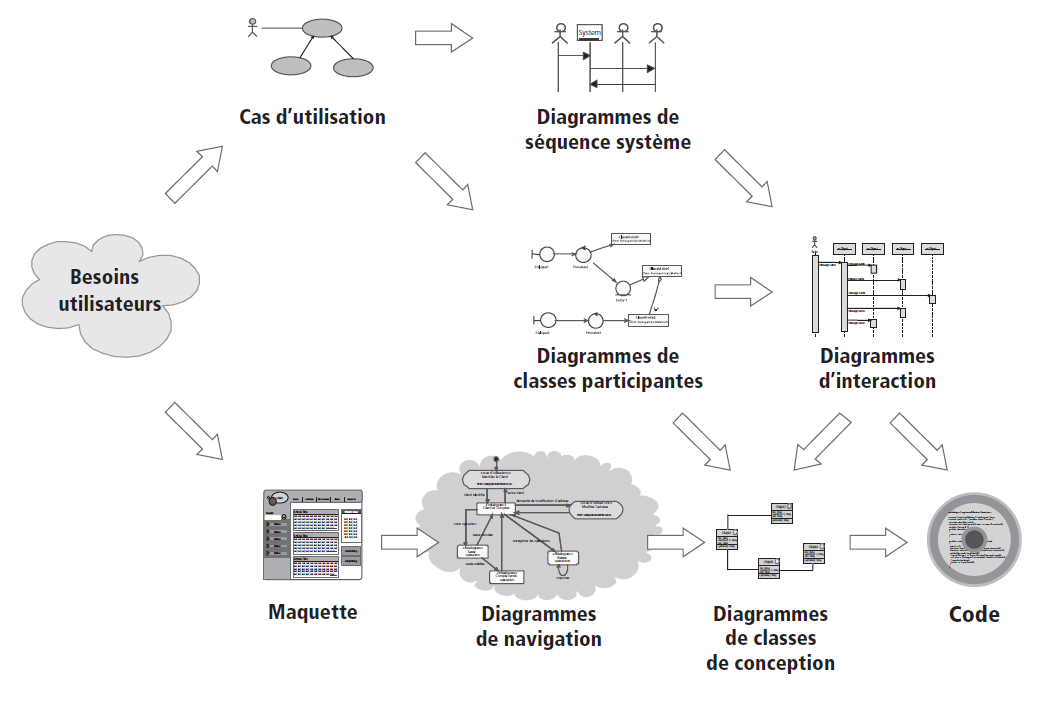
\includegraphics[width=12cm]{images/processus_dev.png}
  \vspace{-10pt}
  \caption{Récapitulatif du processus de développement \cite{5}}
  \label{fig1}
\end{figure}

\vspace{-30pt}
\section{Conclusion}
Ce premier chapitre nous a permis de présenter le cadre général du projet, à
savoir le contexte et la problématique en élaborant une solution à cette
dernière. Nous avons aussi brièvement défini les applications Web et les
empreintes digitales. Nous avons conclu par la description du processus de
développement à suivre tout au long du projet.


%%%% Chapitre 2 %%%%
\chapter{Spécification et analyse des besoins
}
\fancyhead[R]{\textit{Spécification et analyse des besoins}}
\renewcommand{\headrulewidth}{1pt}


\section{Introduction}
Ce chapitre sera consacré à la phase de spécification et d’analyse des besoins.
dans cette étape, nous allons tout d’abord identifier les différents acteurs du
système, ainsi que leurs actions qui sont représentées en cas d’utilisation,
puis nous allons décrire les spécifications des exigences fonctionnelles et non
fonctionnelles, ainsi que leurs contraintes. Ceci nous permettra de modéliser le
diagramme de cas d’utilisation. 

\section{Identification des acteurs}
Un acteur représente une entité extérieure au système modélisé, qui interagit
directement avec lui afin d’atteindre des objectifs \cite{4}. Dans notre
système, on peut identifier 4 acteurs humains :
    
    
\begin{itemize}
    \item[\textbullet] \textbf{L’Employé :} Joue le rôle d’une personne qui
        occupe un emploi dans l’entreprise et qui interagit avec le système,
        pour un pointage des horaires de travail réalisé, ainsi que la
        possibilité de s’authentifier sur la plateforme pour consulter les
        informations qui le concernent.
    \item[\textbullet] \textbf{Le Manager :} Joue le rôle d’un employé très
        important qui est le lien entre la direction et les autres employés. Les
        managers s’occupent de l’organisation et du contrôle de leurs équipes et
        employés à travers la plateforme.
    \item[\textbullet] \textbf{Le Responsable :} Joue le rôle d’un responsable
        qui gère les employés ainsi que les différentes équipes de l’entreprise.
    \item[\textbullet] \textbf{L’administrateur :} Joue le rôle d’une personne
        vitale pour le bon fonctionnement du système via l’espace
        d’administration.
\end{itemize}
    
    
\section{Identifications des cas d'utilisation}
Un cas d’utilisation représente une série d’interactions d’un acteur avec un
système. Cette interaction est destinée à fournir des résultats à l’acteur. Le
tableau ci-dessous présente les différents cas d’utilisations avec leurs acteurs
respectifs.
    
\begin{longtable}{|c|c|c|c|}
    % header and footer information
     \endhead
     \endfoot
    % body of table
     \hline
     \textbf{N}& \multicolumn{2}{c|}{\textbf{Cas d’utilisation}} & \textbf{Acteur}\\
     \hline
     1 & \multicolumn{2}{c|} {S’authentifier} & \multirow{8}{*}{\shortstack{Employé/Manager\\ Responsable}} \\
     \cline{1-3}
     2 & \multicolumn{2}{c|} {Consulter mon tableau de bord} & 
     \\
     \cline{1-3}
     3 & \multicolumn{2}{c|} {Consulter ma fiche de pointage} &
     \\
     \cline{1-3}
     4 & \multicolumn{2}{c|} {Rechercher période} &
     \\
     \cline{1-3}
     5 & \multicolumn{2}{c|} {Consulter mon profile} &
     \\
     \cline{1-3}
     6 & \multicolumn{2}{c|} {Modifier mon profile} &
     \\
     \cline{1-3}
     7 & \multicolumn{2}{c|} {Consulter mon planning} &
     \\
     \cline{1-3}
     8 & \multicolumn{2}{c|} {Se pointer} & 
     \\
     \hline
     9 & \multicolumn{2}{c|} {Consulter tableau de bord manager} &
     \multirow{8}{*}{Manager}\\
     \cline{1-3}
     10 & \multicolumn{2}{c|} {Consulter liste des collaborateurs} &
     \\
     \cline{1-3}
     11 & \multicolumn{2}{c|} {Consulter profil d'un collaborateur} &
     \\
     \cline{1-3}
     12 & \multicolumn{2}{c|} {Consulter planning d'un collaborateur} &
     \\
     \cline{1-3}
     13 & \multicolumn{2}{c|} {Consulter liste de mes équipes} &
     \\
     \cline{1-3}
     14 & \multicolumn{2}{c|} {Consulter résumer de mon équipe} &
     \\
     \cline{1-3}
     15 & \multicolumn{2}{c|} {Consulter résumer de pointage des collaborateurs} &
     \\
     \cline{1-3}
     16 & \multicolumn{2}{c|} {Consulter feuille de pointage d’un collaborateurs} &
     \\
     \hline
     17 & \multicolumn{2}{c|} {Rechercher employé} &
     \multirow{1}{*}{Manager/Responsable}
     \\
     \hline
     18 & \multicolumn{2}{c|} {Consulter le tableau de bord responsable} & \multirow{10}{*}{Responsable}
     \\
     \cline{1-3}
     19 & \multicolumn{2}{c|} {Consulter liste des équipes} & 
     \\
     \cline{1-3}
     20 & \multicolumn{2}{c|} {Consulter résumer d’une équipe} & 
     \\
     \cline{1-3}
     21 & \multicolumn{2}{c|} {Consulter liste des employés} & 
     \\
     \cline{1-3}
     22 & \multicolumn{2}{c|} {Consulter profil d’un employé} & 
     \\
     \cline{1-3}
     23 & \multicolumn{2}{c|} {Consulter liste des plannings} & 
     \\
     \cline{1-3}
     24 & \multicolumn{2}{c|} {Consulter planning d'un employé} & \\
     \cline{1-3}
     25 & \multicolumn{2}{c|} {Consulter résumer de pointage des employés} & \\
     \cline{1-3}
     26 & \multicolumn{2}{c|} {Consulter feuille de pointage d’un employé} & \\
     \cline{1-3}
     27 & \multicolumn{2}{c|} {Consulter journal d'affectation} & \\
     \hline
     \multirow{4}{*}{28} & \multirow{4}{*}{Gérer les plannings}   &{Ajouter un planning} &  \\
     & & {Modifier un planning} & \\
     & & {Supprimer un planning} & \\
     & & {Affectation d'un planning} & \\
     \cline{1-3}
     \multirow{5}{*}{29} & \multirow{5}{*}{Gérer les équipes}   &{Ajouter une équipe} & \multirow{2}{*}{Responsable/Administrateur} \\
     & & {Modifier une équipe} & \\
     & & {Supprimer une équipe} & \\
     & & {Ajouter membre} & \\
     & & {Supprimer membre} & \\
     \hline
     30 & \multicolumn{2}{c|} {Importer/exporter} & \multirow{6}{*}{Responsable/Administrateur}  \\
     \cline{1-3}
     31 & \multicolumn{2}{c|} {Ajouter une empreinte} & \\
     \cline{1-3}
     32 & \multicolumn{2}{c|} {Supprimer une empreinte} & \\
     \cline{1-3}
     \multirow{3}{*}{33} & \multirow{3}{*}{Gérer les employés}   &{Ajouter un employé} & \\
     & & {Modifier un employé} & \\
     & & {Supprimer un employé} & \\
     \hline
\end{longtable}


\section{Spécification des exigences}

\subsection{Exigences fonctionnelles}
Les besoins fonctionnels expriment une action que doit effectuer le système en
réponse à une demande (sorties qui sont produites pour un ensemble donné
d’entrées). Par exemple, le système doit stocker les informations de pointage des
employés. Le système à concevoir devra répondre aux besoins que nous allons
citer. Afin de mettre en évidence les différentes informations accessibles selon
le rôle, nous avons décidé de les regrouper par acteur.

\begin{itemize}
    \item [\textbullet] \textbf{Employé :} Accès à son profil ainsi qu’aux
        informations de pointage et au planning qui le concerne, ainsi qu’aux
        informations publiques et aux statuts de présence des collaborateurs
        faisant partie de la même équipe que lui.
        
    \item [\textbullet] \textbf{Manager :} En plus des informations accessibles
        à l’employé, le manager doit avoir accès aux informations des équipes
        dont il est responsable ainsi qu’aux informations des membres qui les
        composent, aux plannings et aux informations de pointage y compris.

    \item [\textbullet] \textbf{Responsable :} Celui-ci doit avoir accès à la
        totalité des informations du système concernant tous les employés, quels
        que soient leurs statuts. Il doit être capable d’ajouter, modifier,
        supprimer des équipes ou des plannings, affecter un manager à une
        équipe, un planning à un employé, ajouter ou supprimer un employé à
        une équipe. Importer/exporter des informations de pointage est une
        fonctionnalité primordiale que doit avoir ce rôle.
        
    \item [\textbullet] \textbf{Administrateur :} La personne responsable de
        maintenir le système et de veiller à son bon fonctionnement a
        naturellement accès à l’espace d’administration du système à partir
        duquel elle pourra gérer les comptes des différents utilisateurs et leur
        assigner le bon rôle. En cas d’incohérences ou d’erreurs, ce dernier
        devrait avoir la possibilité d’intervenir de manière directe sur la base
        de données afin de résoudre ces cas. Ce dernier doit pouvoir aussi gérer
        les empreintes (ajout et suppression).
\end{itemize}

En plus des besoins précédemment cités, il existe des besoins partagés entre
tous les acteurs tels que :

\begin{itemize}
    \item [\textbullet] Authentification : Chaque utilisateur du futur système
        devrat être authentifié au préalable avec son nom d’utilisateur et son
        mot de passe avant tout accès à ce dernier. Le système devrait ensuite
        rediriger l’utilisateur vers son espace utilisateur qui varie selon son
        rôle.

    \item [\textbullet] Récupérations de mot de passe : Tous les utilisateurs
        pourront réinitialiser leurs mots de passe grâce à leurs adresses mail.
\end{itemize}
            
\subsection{Exigences non fonctionnelles}
Ce sont des besoins qui caractérisent le système, elles sont liées aux
contraintes pesant sur les fonctionnalités. La liste suivante représente les
besoins non fonctionnels de notre système :

\begin{itemize}
    \item [\textbullet] Performance : l’application doit assurer un temps de
        réponse minime, tout en répondant aux exigences de l’utilisateur.
    
    \item [\textbullet] Sécurité : aucune opération ne doit être possible sans
        authentification préalable. Une protection contre CSRF est impérative.
        Les informations doivent être accessibles aux utilisateurs possédant les
        bons droits d’accès seulement. Les mots de passe doivent être hashés
        puis stockés et jamais stockés en clair. Le système doit identifier la
        pointeuse afin d’accepter les informations reçues.
    
    \item [\textbullet] Ergonomie : les informations doivent êtres lisibles et
        facilement interprétables. Des graphiques résumant les informations
        pertinentes doivent être présentés à l’utilisateur. Une navigation
        simple et efficace. L’utilisation d’icônes explicites permettant de
        comprendre le sens des actions que l’utilisateur s’apprête à effectuer.
        Les actions critiques doivent toujours être confirmées avant leurs
        exécutions. Le système ne doit pas nécessiter une formation longue durée
        pour être utilisé, il doit offrir une prise en main rapide et facile
        sans beaucoup d’efforts.
    
     \item [\textbullet] Modularité du code : contenu du contexte et de la
         problématique traitée. On se doit de penser à l’évolution potentielle
         du système. Dans cette optique, il est primordial d’écrire un code
         lisible, modulaire et bien documenté pour faciliter la maintenance, la
         personnalisation, et l’évolutivité de la solution proposée.
\end{itemize}
                

\section{Diagramme des cas d'utilisation}
Les diagrammes de cas d’utilisation représentent la structure des
fonctionnalités nécessaires aux utilisateurs du système \cite{6}, nous allons
ici modéliser les diagrammes de cas d’utilisation des 4 acteurs du système pour
avoir une vue globale de ce dernier.

\clearpage  
\subsection{Diagramme de cas d'utilisation de l'employé}
    \begin{figure}[h!]
        \centering
        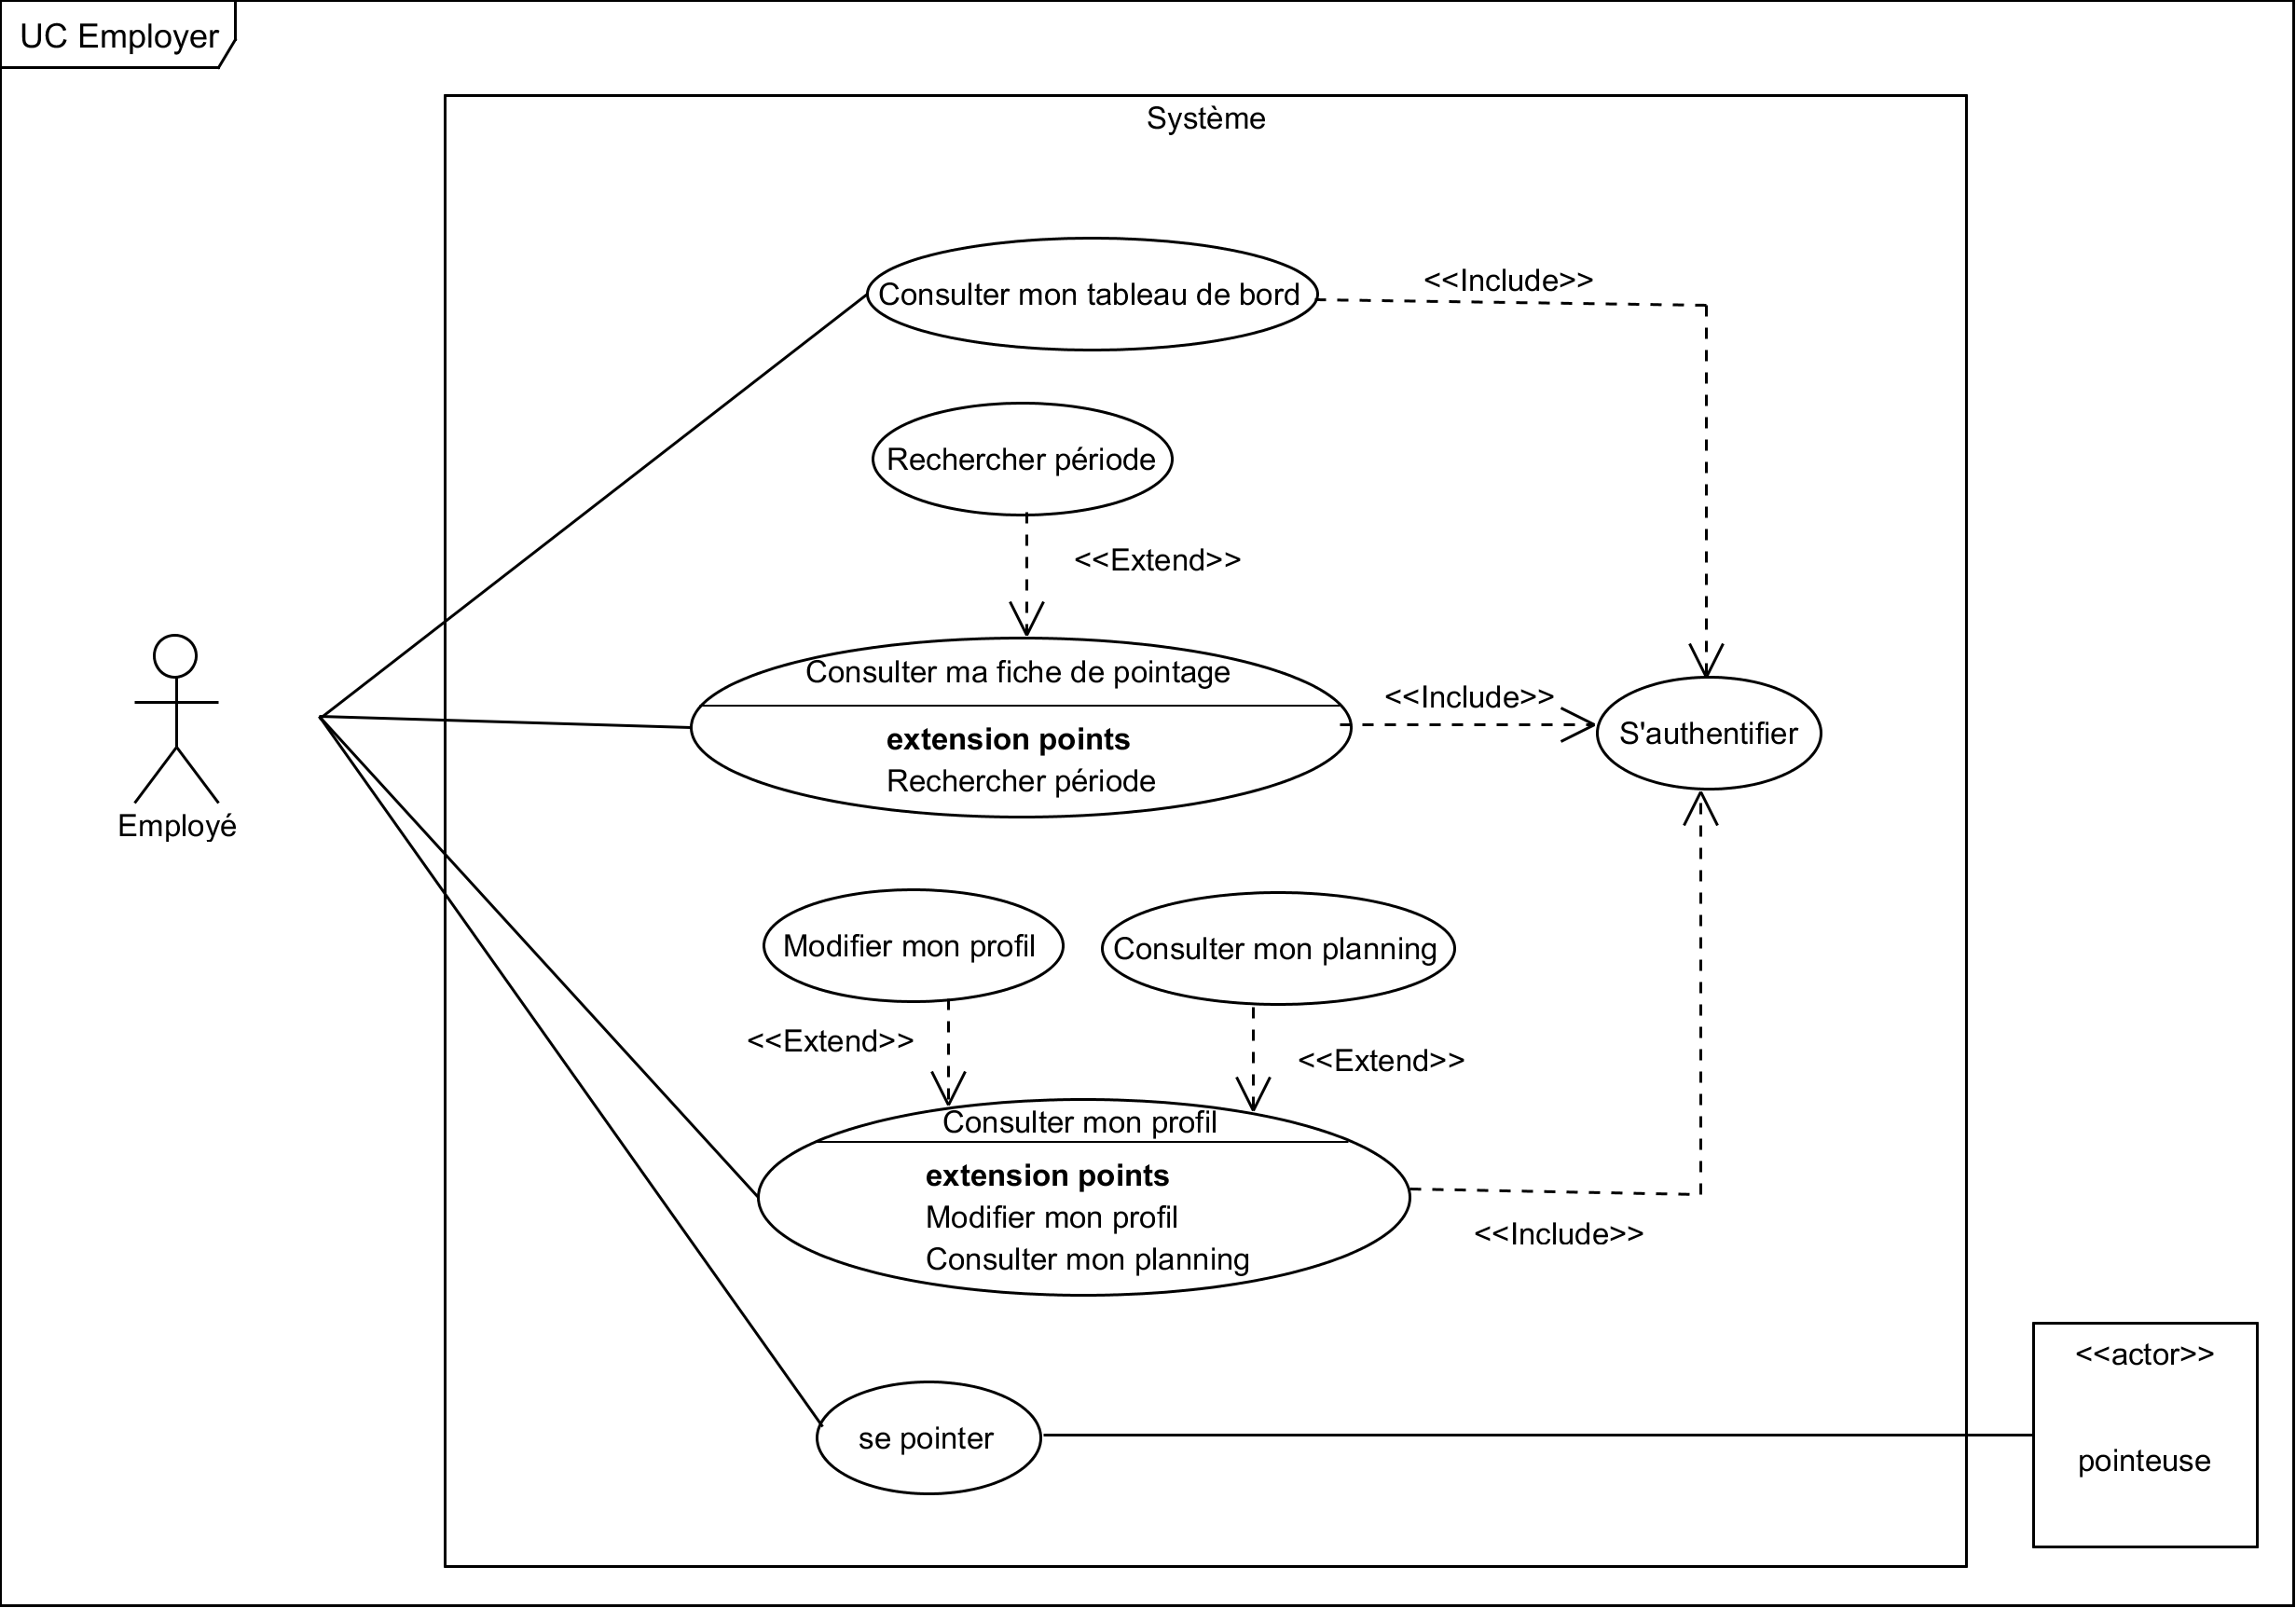
\includegraphics[angle=90, height=21cm]{images/uc_employe.png}
        \caption{Diagramme de cas d'utilisation associé à l'acteur «Employé»}
        \label{fig2}
    \end{figure}
    
\subsection{Diagramme de cas d'utilisation du manager}
    \begin{figure}[h!]
        \centering
        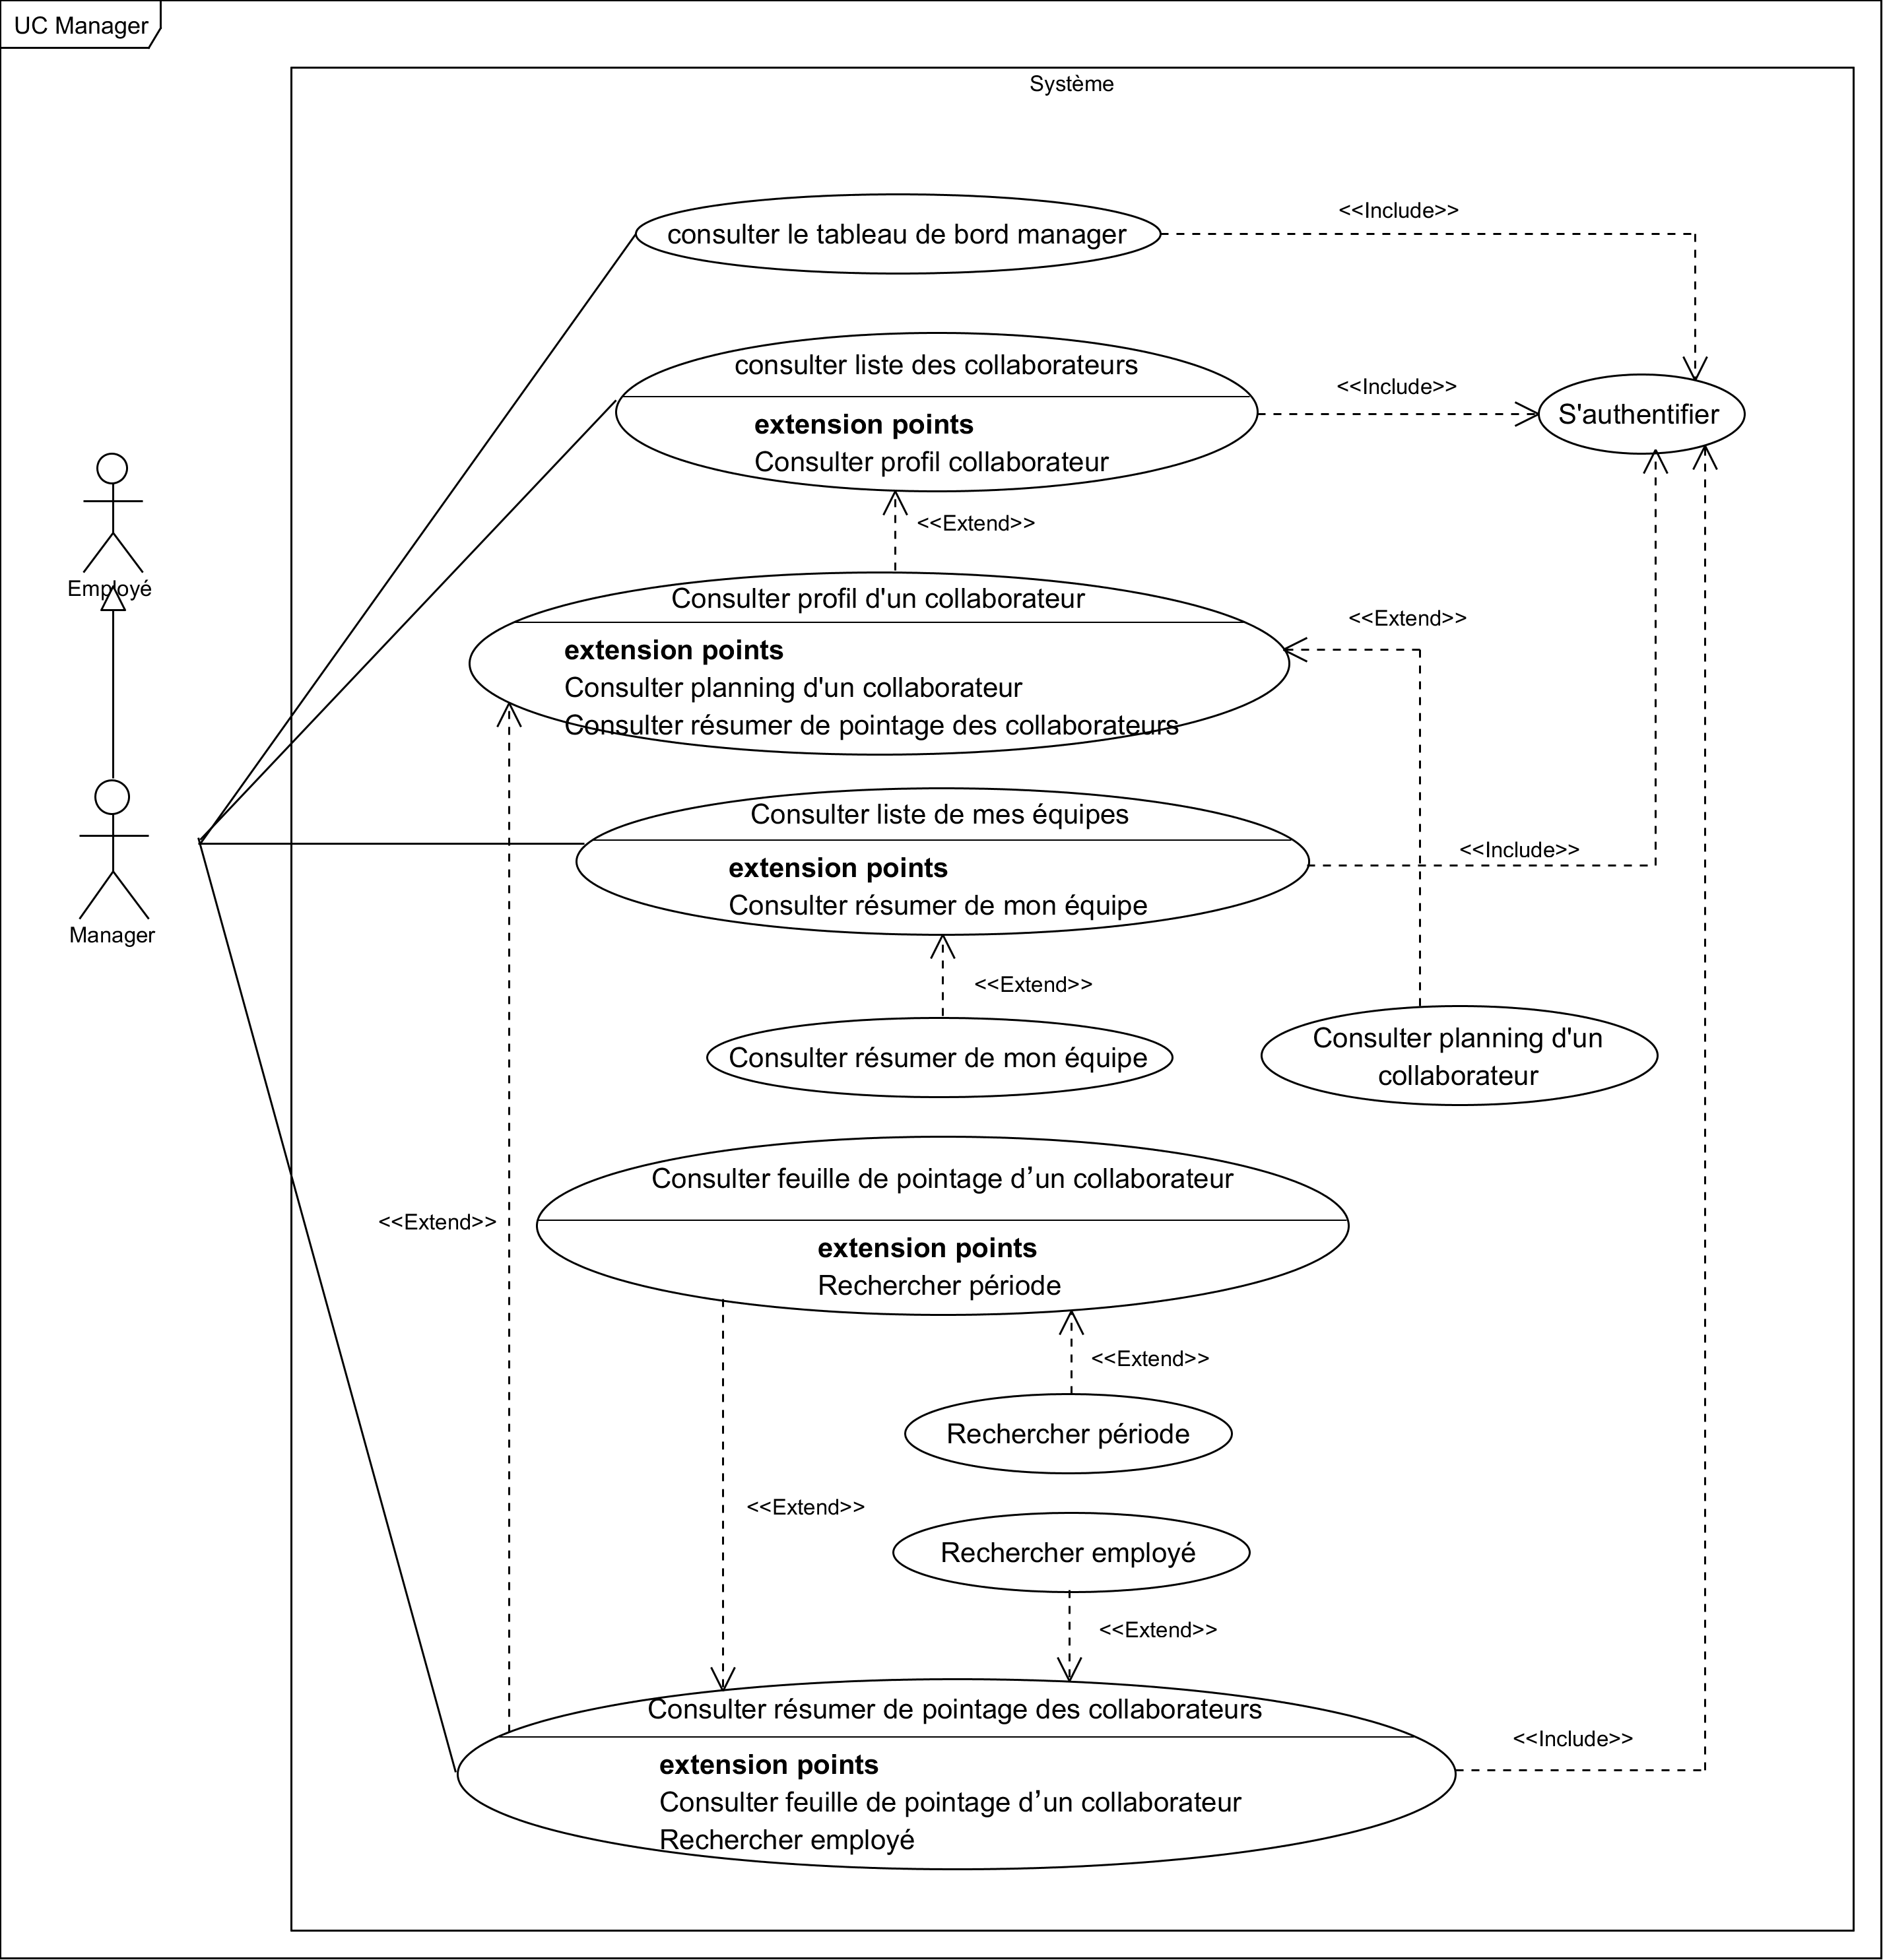
\includegraphics[width=16cm,height=21cm]{images/uc_manager.png}
        \caption{Diagramme de cas d'utilisation associé à l'acteur «Manager»}
        \label{fig3}
    \end{figure}

\clearpage  
 
\subsection{Diagramme de cas d'utilisation du responsable}
    \begin{figure}[h!]
         \centering
         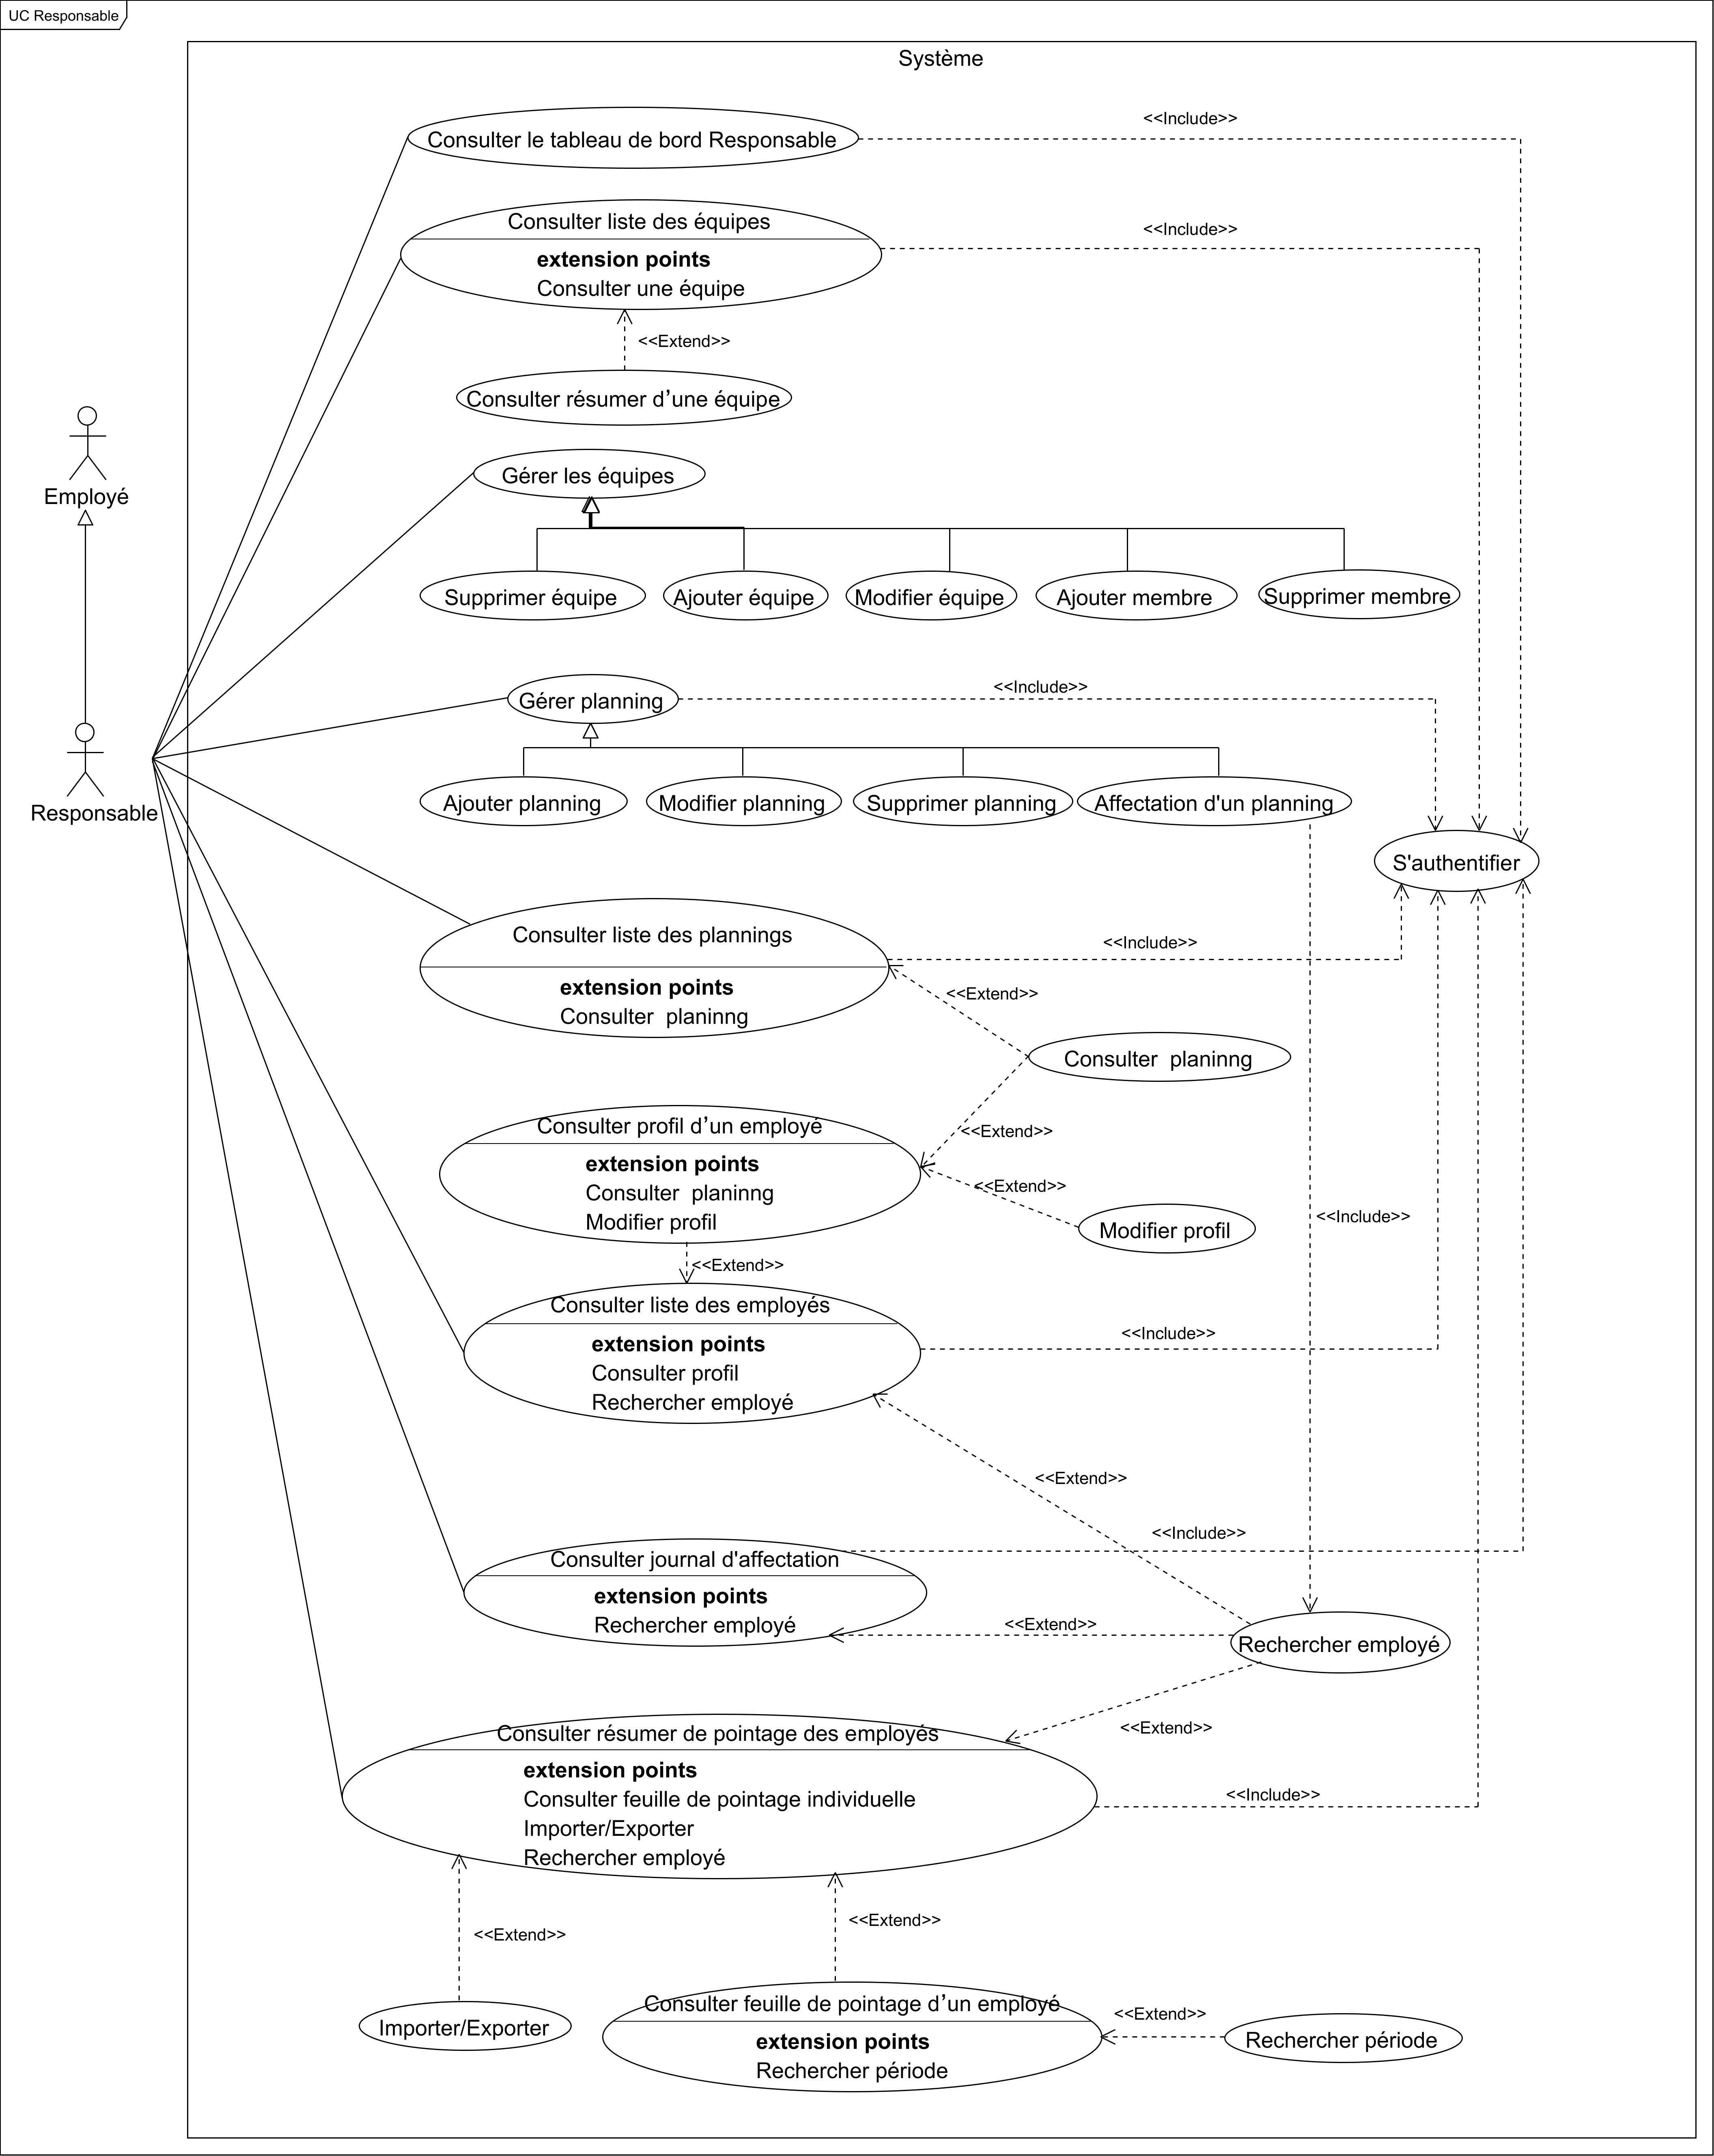
\includegraphics[width=17cm,height=21cm]{images/uc_responsable.png}
         \caption{Diagramme de cas d'utilisation associé à l'acteur «Responsable»}
         \label{fig4}
    \end{figure}
    
\clearpage  
 
\subsection{Diagramme de cas d'utilisation de l'administrateur}
    \begin{figure}[h!]
         \centering
         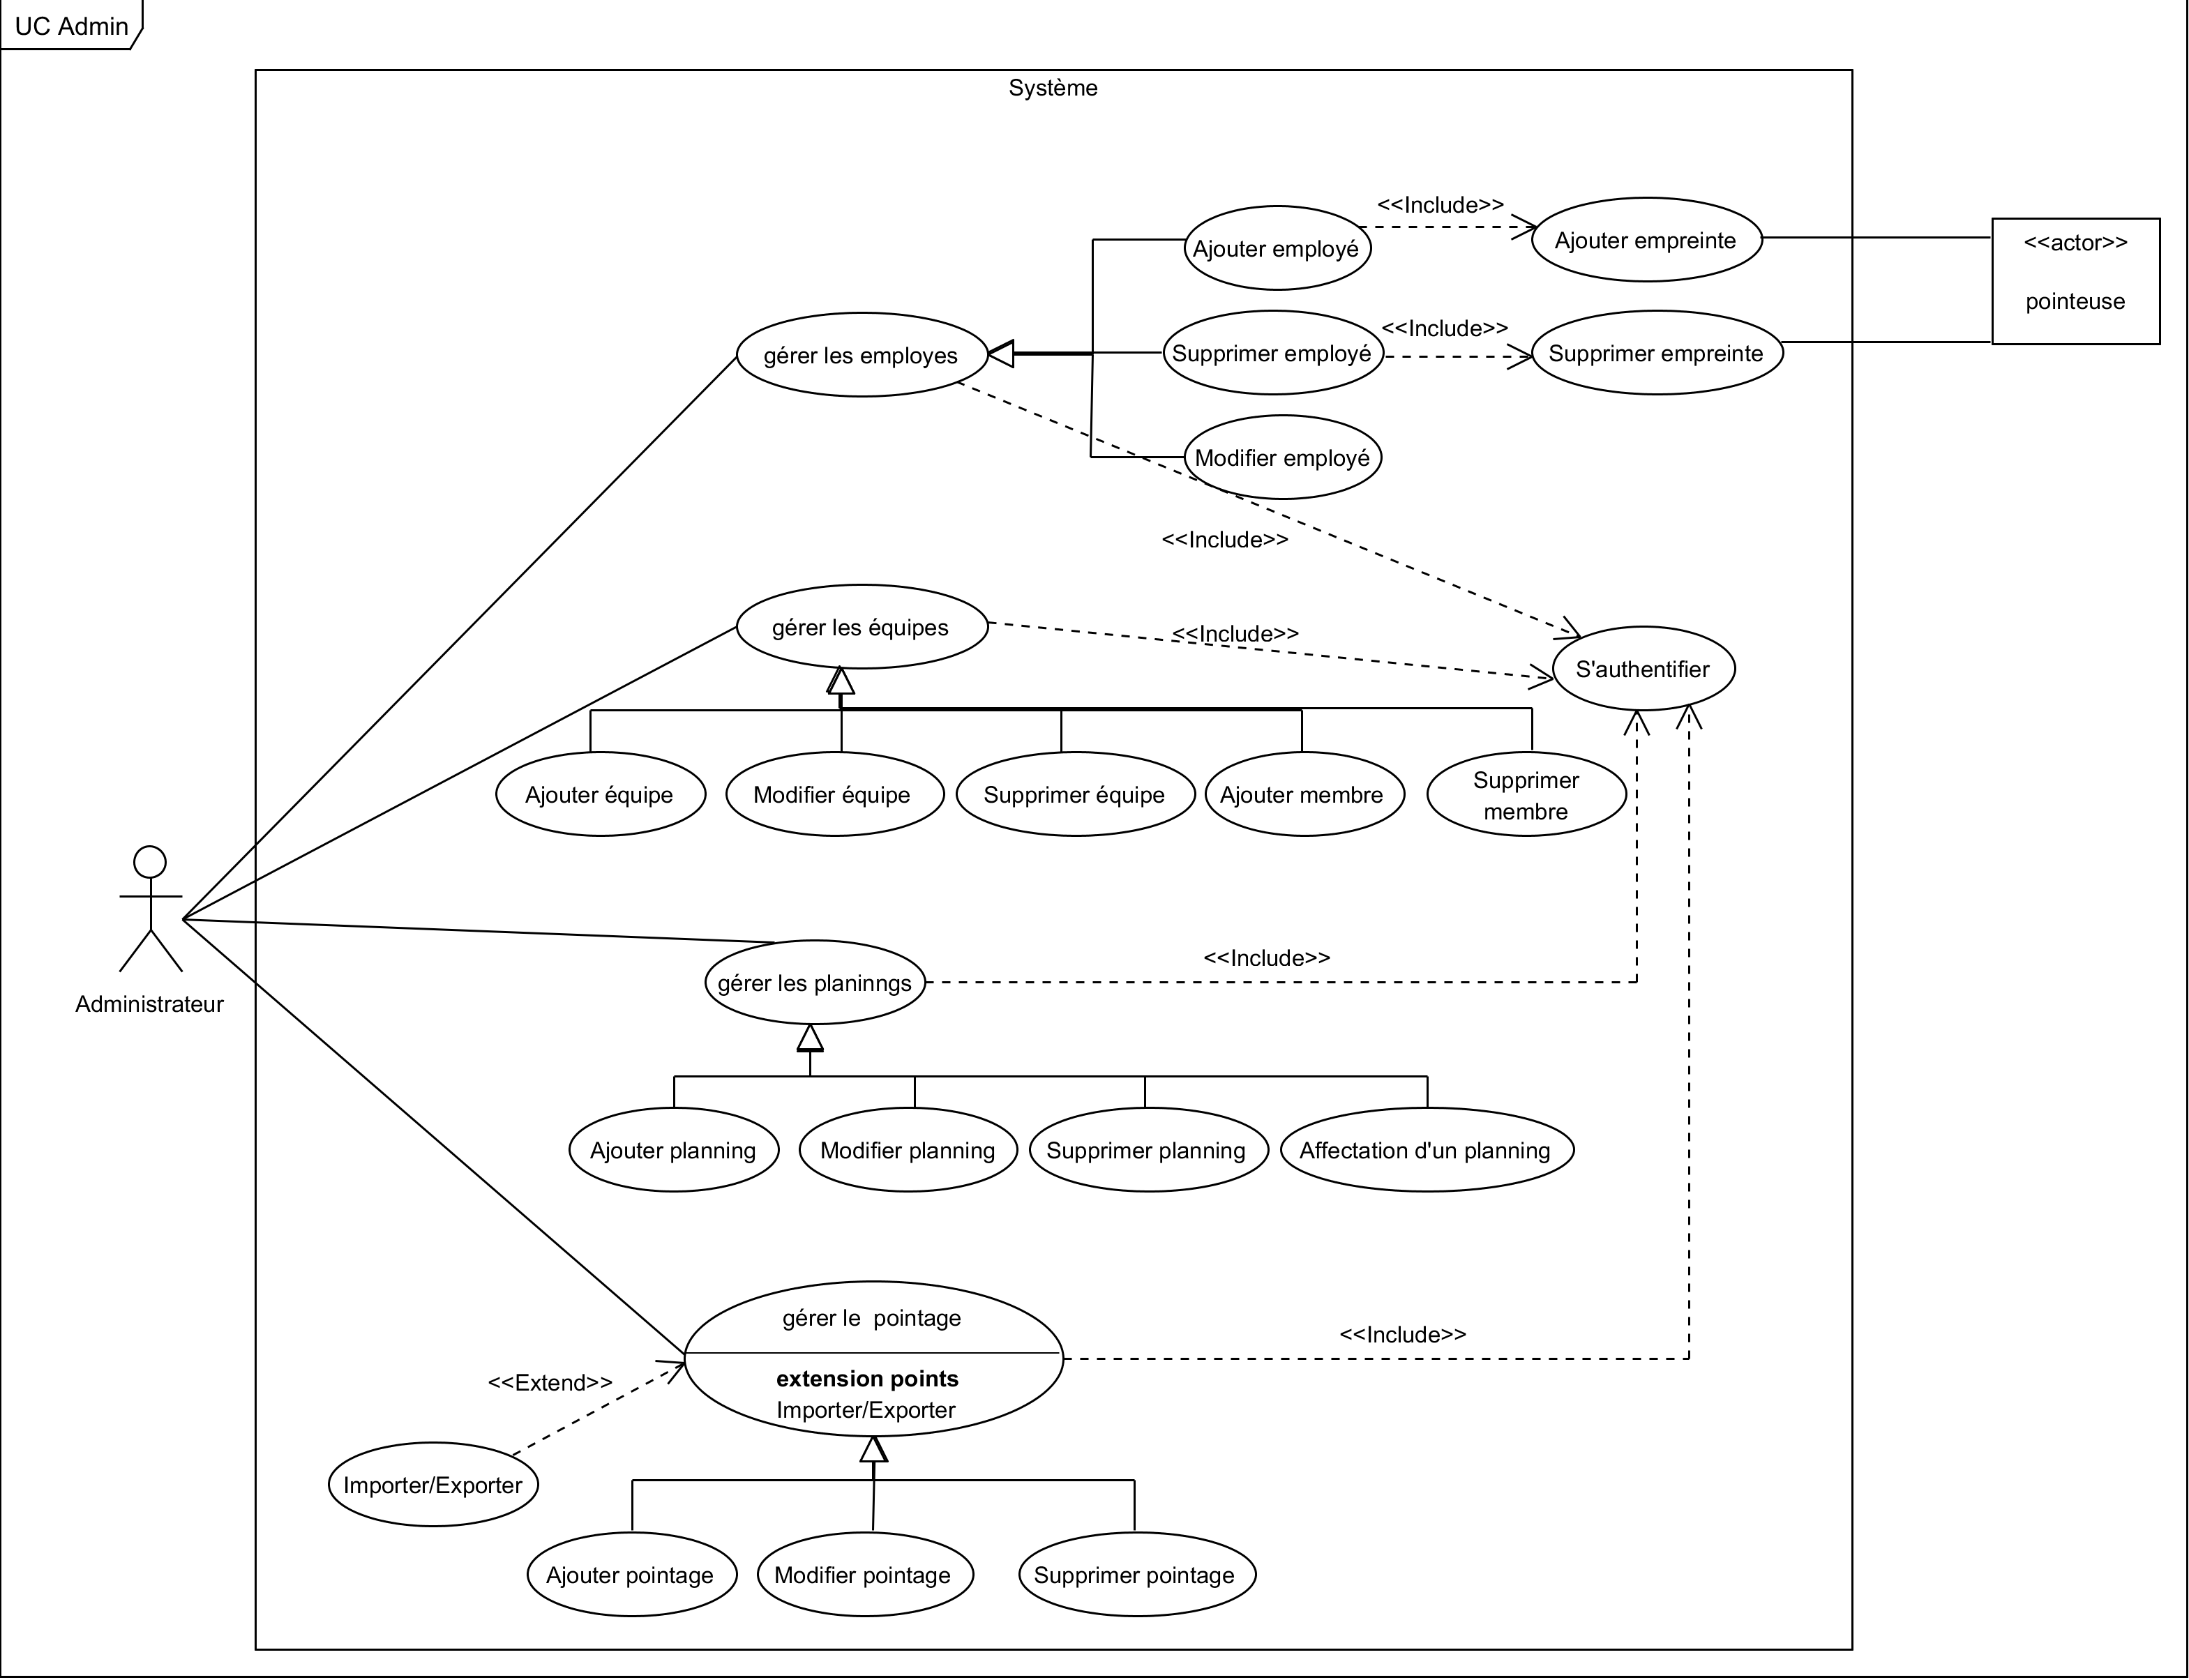
\includegraphics[angle=90, height=21cm]{images/uc_admin.png}
         \caption{Diagramme de cas d'utilisation associé à l'acteur «Administrateur»}
         \label{fig5}
    \end{figure}

\clearpage
\textcolor{red}{
L’objectif de certains cas d’utilisation est même en surface néanmoins ils sont
exécutés par des acteurs différents et dans des champs d’action distincts. On
peut illustrer ça avec le cas d’utilisation « Consulter mon profil », «
Consulter profil d’un collaborateur » et « Consulter profil d’un employé ». 
}

Le premier cas concerne un employé qui consulte son propre profil en ayant la
possibilité de modifier certaines informations. Le deuxième cas est déclenché
par le manager pour consulter le profil d’un collaborateur sans pouvoir le
modifier. Le troisième est utilisé par un administrateur pour consulter le
profil d’un employé (quel que soit son rôle) avec la possibilité de modifier
toutes les informations. 

\section{Descriptions de cas d'utilisation}
Les cas d’utilisation ne représentent pas uniquement les interactions avec les
acteurs, mais ils ajoutent également les prés et post conditions ainsi que les
enchaînements alternatifs. Dans cette partie, nous allons décrire les diagrammes
de cas d’utilisation des différents acteurs.
    
\subsection*{Cas d'utilisation « S'authentifier »}

\begin{longtable}{|p{4cm}|p{12cm}|}
    % header and footer information
    \endhead
    \endfoot
    % body of table
    \hline
    \multicolumn{2}{|c|}{\textbf{Sommaire d’identification}} \\
    \hline
    Titre & \textbf{S'authentifier} \\
    \hline
    Acteur & Employé, Manager, Responsable, Administrateur \\
    \hline
    Résumer & L’acteur doit s’identifier en saisissant son nom d'utilisateur et mot de passe pour accéder a son espace personnel. \\
    \hline
    \multicolumn{2}{|c|}{Description des scénarios} \\
    \hline
    Pré-conditions &  L’utilisateur doit être créé par l'administrateur. \\
    \hline
    Scénario nominal &  
    \begin{minipage}[t]{\linewidth}
        \begin{enumerate}[itemindent=0pt, leftmargin=*, nosep,before=\vspace{-0.5\baselineskip}]
            \item Le système affiche le formulaire d'authentification.
            \item L'acteur saisit le nom d'utilisateur ainsi que son mot de passe.
            \item Le système vérifie si les identifiants saisis sont corrects.
            \item Le système affiche le tableau de bord (voir le cas d’utilisations « Consulter mon tableau de bord »)
        \end{enumerate}
    \end{minipage}
    \\
    \hline
    Enchaînement alternatif &  
    \begin{minipage}[t]{\linewidth}
        2a. Les identifiants saisis par l'acteur sont incorrects.
        \begin{enumerate}[nosep,after=\strut]
            \item Le système affiche un message d'erreur pour signaler que les identifiants sont incorrects.
            \item Le cas d’utilisation reprend de l’étape 1 du scénario nominale.
        \end{enumerate}
    \end{minipage}
    \hline
    Postconditions & L'utilisateur est authentfié et accède aux fonctionnalités qui lui sont dédiées.  \\
    \hline
    \caption{Description du cas d'utilisation « S'authentifier »}\\
\end{longtable}

\subsection*{Cas d'utilisation « Se pointer »}
\begin{longtable}{|p{4cm}|p{12cm}|}
    % header and footer information
    \endhead
    \endfoot
    % body of table
    \hline
    \multicolumn{2}{|c|}{\textbf{Sommaire d’identification}} \\
    \hline
    Titre & \textbf{Se pointer} \\
    \hline
    Acteur & Employé, Manager, Responsable, Pointeuse  \\
    \hline
    Résumer & Un acteur signale son entrée ou sa sortie de l'entreprise en posant son index sur la pointeuse. \\
    \hline
    \multicolumn{2}{|c|}{Description des scénarios} \\
    \hline
    Pré-conditions & Être enregistrer dans le système (empreinte et profile)  \\
    \hline
    Scénario nominal &   

    \begin{minipage}[t]{\linewidth}
        \begin{enumerate}[itemindent=0pt, leftmargin=*, nosep,before=\vspace{-0.5\baselineskip}]
            \item L’acteur pose son index sur le lecteur d'empreinte.
            \item La pointeuse reconnait l’acteur et envoie un signal au système.
            \item Le système accuse la réception du signal.
            \item La pointeuse reçoit un accusé de réception et fait clignoter une LED, pour signaler le bon déroulement de l’opération de pointage.
        \end{enumerate}
    \end{minipage}
    \\
    \hline
    Enchaînement alternatif &   
    \begin{minipage}[t]{\linewidth}
        2a La pointeuse ne reconnait pas l’acteur.
        \begin{enumerate}[nosep,after=\strut]
            \item La LED de la pointeuse ne clignotera pas.
            \item Le cas d’utilisation reprend de l’étape 1 du scénario nominale.
        \end{enumerate}
    \end{minipage}
    \\
    \hline
    Postconditions &  Le système enregistrent l’heure et l’ID de l’employé responsable de l’événement. \\
    \hline
    Postconditions &   \\
    \hline
    \caption{Description du cas d'utilisation « Se pointer »}\\
\end{longtable}        
        
\subsection*{Cas d'utilisation « Consulter mon profil »}
\begin{longtable}{|p{4cm}|p{12cm}|}
    % header and footer information
    \endhead
    \endfoot
    % body of table
    \hline
    \multicolumn{2}{|c|}{\textbf{Sommaire d’identification}} \\
     \hline
     Titre & \textbf{Consulter mon profil} \\
     \hline
        Acteur & Employé, Manager, Responsable \\
        \hline
        Résumer & L’acteur accède aux informations qui constitue son profile. \\
        \hline
        \multicolumn{2}{|c|}{Description des scénarios} \\
        \hline
        Pré-conditions &  Être authentifier. \\
        \hline
        Scénario nominal & 
        \begin{minipage}[t]{\linewidth} \begin{enumerate}[itemindent=0pt, leftmargin=*, nosep,after=\vspace{-\baselineskip},before=\vspace{-0.5\baselineskip}]
            \item Les différentes informations du profile son afficher.
        \end{enumerate}
        \end{minipage}
         \\
        \hline
        Enchaînement alternatif &  
        1a. L’employé peut modifier ses informations (voir le cas d’utilisations « modifier mon profile »)
        \\
        
        \hline
        Postconditions &   \\
        \hline
        \caption{Description du cas d'utilisation « Consulter mon profil »}\\
\end{longtable}        
        
\subsection*{Cas d'utilisation « Consulter ma fiche de pointage »}
\begin{longtable}{|p{4cm}|p{12cm}|}
        % header and footer information
        \endhead
        \endfoot
        % body of table
        \hline
         \multicolumn{2}{|c|}{\textbf{Sommaire d’identification}} \\
         \hline
         Titre & \textbf{Consulter ma fiche de pointage} \\
         \hline
            Acteur & Employé, Manager, Responsable \\
            \hline
            Résumer &  L’acteur accède aux informations relatives à son pointage (Heures d’arrivée et de sortie) \\
            \hline
            \multicolumn{2}{|c|}{Description des scénarios} \\
            \hline
            Pré-conditions & Être authentifier.  \\
            \hline
            Scénario nominal &  
            \begin{minipage}[t]{\linewidth}
                \begin{enumerate}[itemindent=0pt, leftmargin=*, nosep,after=\vspace{-\baselineskip},before=\vspace{-0.5\baselineskip}]
                      \item Le système affiche les informations de pointage de l’acteur concerné pour une semaine.
                      \\\\
                      
                \end{enumerate}
            \end{minipage}
            \\
            \hline
            Enchaînement alternatif & 
            \begin{minipage}[t]{\linewidth}
                1a. l'acteur choisi d'avoir un affichage par mois.
                \begin{enumerate}[nosep,after=\strut]
                      \item Le système affiche les informations de pointage de l’acteur concerné pour un mois.
                \end{enumerate}
            \end{minipage}
            \\
            
            \hline
            Postconditions &   \\
            \hline
        \caption{Description du cas d'utilisation « Consulter ma fiche de pointage »}\\
\end{longtable}
            
\subsection*{Cas d'utilisation « Consulter tableau de bord manager »}
\begin{longtable}{|p{4cm}|p{12cm}|}
    % header and footer information
    \endhead
    \endfoot
    % body of table
    \hline
     \multicolumn{2}{|c|}{\textbf{Sommaire d’identification}} \\
     \hline
     Titre & \textbf{Consulter tableau de bord manager} \\
     \hline
        Acteur & Manager \\
        \hline
        Résumer & Le manager consulte son tableau de bord, qui est constitué de deux parties.La première représente le tableau de bord du manager en tan que employé tendis que la deuxième qui est un récapitulatif des informations de pointage de son/ses équipes et de tous ses collaborateurs). \\
        \hline
        \multicolumn{2}{|c|}{Description des scénarios} \\
        \hline
        Pré-conditions &  Le manager doit être authentifié. \\
        \hline
        Scénario nominal &  
            \begin{minipage}[t]{\linewidth}
                \begin{enumerate}[itemindent=0pt, leftmargin=*, nosep,before=\vspace{-0.5\baselineskip}]
                      \item Le système affiche un résumé des informations de pointage concernant le manager et son planning du jour.
                \end{enumerate}
            \end{minipage}
        \\
        \hline
        Enchaînement alternatif & 
            \begin{minipage}[t]{\linewidth}
            1a. Le manager décide de consulter la deuxième partie de son tableau de bord.
             \begin{enumerate}[nosep,after=\strut]
                      \item Le système affiche la partie qui concerne ses équipes ainsi que les collaborateurs encadrés par le manager en question.
                \end{enumerate}
            \end{minipage}
        \\
        
        \hline
        Postconditions &   \\
        \hline
    \caption{Description du cas d'utilisation « Consulter tableau de bord manager »}\\
\end{longtable}        
        
\subsection*{Cas d'utilisation « Ajouter membre »}
\begin{longtable}{|p{4cm}|p{12cm}|}
    % header and footer information
    \endhead
    \endfoot
    % body of table
    \hline
    \multicolumn{2}{|c|}{\textbf{Sommaire d’identification}} \\
     \hline
     Titre & \textbf{Ajouter membre} \\
     \hline
        Acteur & Responsable, Administrateur \\
        \hline
        Résumer & L’acteur accède à une interface qui lui permet d'affecter des employés à l'équipe'. \\
        \hline
        \multicolumn{2}{|c|}{Description des scénarios} \\
        \hline
        Pré-conditions &  Être authentifier. \\
        \hline
        Scénario nominal & 
        \begin{minipage}[t]{\linewidth} \begin{enumerate}[itemindent=0pt, leftmargin=*, nosep,after=\vspace{-\baselineskip},before=\vspace{-0.5\baselineskip}]
            \item L'acteur recherche un employé (voir le cas d’utilisations \underline{Recherche employé }).
            \item Le système retourne une liste d'employés.
            \item L'acteur sélectionne un employé et l'ajoute.
            \item Le système affiche l'interface d'affectation avec les données mise à jour.\\\\
        \end{enumerate}
        \end{minipage}
         \\
        \hline
        Enchaînement alternatif &  
        \begin{minipage}[t]{\linewidth}
            2a. Aucun employé trouver. \begin{enumerate}[nosep,after=\strut]
                  \item Le système affiche un message d'erreur.
            \end{enumerate}
        \end{minipage}
        \\
        
        \hline
        Postconditions &   \\
        \hline
        \caption{Description du cas d'utilisation « Ajouter membre »}\\
\end{longtable}        
        
\subsection*{Cas d'utilisation « Ajouter un planning »}  
\begin{longtable}{|p{4cm}|p{12cm}|}
        % header and footer information
        \endhead
        \endfoot
        % body of table
        \hline
        \multicolumn{2}{|c|}{\textbf{Sommaire d’identification}} \\
         \hline
         Titre & \textbf{Ajouter équipe} \\
         \hline
            Acteur & Responsable, Administrateur \\
            \hline
            Résumer & L’acteur accède à une interface qui lui permet la création d'un nouveau planning. \\
            \hline
            \multicolumn{2}{|c|}{Description des scénarios} \\
            \hline
            Pré-conditions &  Être authentifier. \\
            \hline
            Scénario nominal & 
            \begin{minipage}[t]{\linewidth} \begin{enumerate}[itemindent=0pt, leftmargin=*, nosep,after=\vspace{-\baselineskip},before=\vspace{-0.5\baselineskip}]
                \item Le système affiche le formulaire.
                \item L'acteur saisit le nom du planning ainsi que la description et les horaires de travail.
                \item Le système vérifie la conformité des informations saisie.
                \item Le système affiche la liste des plannings voir cas d'utilisations \underline{ Consulter liste des plannings}.\\\\
            \end{enumerate}
            \end{minipage}
             \\
            \hline
            Enchaînement alternatif &  
            \begin{minipage}[t]{\linewidth}
                2a. Le nom de l'équipe est déjà existant.
                \begin{enumerate}[nosep,after=\strut]
                      \item Le système affiche un message d'erreur pour signaler que le nom du planning existe dans la base de données.
                      \item Le cas d’utilisation reprend de l’étape 1 du scénario nominale.
                \end{enumerate}
            \end{minipage}
            \\
            
            \hline
            Postconditions &   \\
            \hline
            \caption{Description du cas d'utilisation « Ajouter un planning »}\\
\end{longtable}        
        
\subsection*{Cas d'utilisation « Ajouter équipe »}  
    \begin{longtable}{|p{4cm}|p{12cm}|}
            % header and footer information
            \endhead
            \endfoot
            % body of table
            \hline
            \multicolumn{2}{|c|}{\textbf{Sommaire d’identification}} \\
             \hline
             Titre & \textbf{Ajouter équipe} \\
             \hline
                Acteur & Responsable, Administrateur \\
                \hline
                Résumer & L’acteur accède à une interface qui lui permet la création d'une nouvelle équipe. \\
                \hline
                \multicolumn{2}{|c|}{Description des scénarios} \\
                \hline
                Pré-conditions &  Être authentifier. \\
                \hline
                Scénario nominal & 
                \begin{minipage}[t]{\linewidth} \begin{enumerate}[itemindent=0pt, leftmargin=*, nosep,after=\vspace{-\baselineskip},before=\vspace{-0.5\baselineskip}]
                    \item Le système affiche le formulaire.
                    \item L'acteur saisit le nom de l'équipe ainsi que la description et sélectionne le manager de cette dernière.
                    \item Le système vérifie la conformité des informations saisie.
                    \item Le système affiche l'interface d'affectation des membres de l'équipe (voir le cas d’utilisations « affectation des membres »).\\\\
                \end{enumerate}
                \end{minipage}
                 \\
                \hline
                Enchaînement alternatif &  
                \begin{minipage}[t]{\linewidth}
                    2a. Le nom de l'équipe est déjà existant.
                    \begin{enumerate}[nosep,after=\strut]
                          \item Le système affiche un message d'erreur pour signaler que le nom de l'équipe existe dans la base de données.
                          \item Le cas d’utilisation reprend de l’étape 1 du scénario nominale.
                    \end{enumerate}
                \end{minipage}
                \\
                
                \hline
                Postconditions &   \\
                \hline
                \caption{Description du cas d'utilisation « Ajouter équipe »}\\
        \end{longtable}        
        
\subsection*{Cas d'utilisation « Ajouter un employé  »}
        \begin{longtable}{|p{4cm}|p{12cm}|}
            % header and footer information
            \endhead
            \endfoot
            % body of table
            \hline
            \multicolumn{2}{|c|}{\textbf{Sommaire d’identification}} \\
            \hline
            Titre & \textbf{Ajouter un employé} \\
             \hline
                Acteur &  Administrateur\\
                \hline
                Résumer &  L’administrateur ajoute un employé.\\
                \hline
                \multicolumn{2}{|c|}{Description des scénarios} \\
                \hline
                Pré-conditions &  Être authentifier   \\
                \hline
                Scénario nominal &  
                \begin{minipage}[t]{\linewidth}
                        \begin{enumerate}[itemindent=0pt, leftmargin=*, nosep,before=\vspace{-0.5\baselineskip},after=\vspace{0.2\baselineskip}]
                            \item L’administrateur saisit l’ensemble des informations de l’employé.
                            \item L’administrateur enregistre l’employé.
                            \item L’administrateur enregistre l’empreinte de l’employé (Cas d’utilisation \underline{Ajouter une empreinte}).
                        \end{enumerate}
                \end{minipage}
                \\
                \hline
                Enchaînement alternatif & 
                \begin{minipage}[t]{\linewidth}
                        2a Les informations saisies ne sont pas valides.
                        \begin{enumerate}[nosep,after=\strut, leftmargin=*]
                            \item Le système affiche un message qui spécifie les informations incorrectes et demande au responsable de les corriger.
                            \item Le cas d’utilisation reprend de l’étape 1 du scénario nominal.
                        \end{enumerate}
                \end{minipage}
                \\
                
                \hline
                Postconditions & Mise à jour des données présentes dans la base de données.
                \\
                \hline
                \caption{Description du cas d'utilisation « Ajouter un employé »}\\
        \end{longtable}        
        
\subsection*{Cas d'utilisation « Consulter profil d'un employé »}
        \begin{longtable}{|p{4cm}|p{12cm}|}
            % header and footer information
            \endhead
            \endfoot
            % body of table
            \hline
                 \multicolumn{2}{|c|}{\textbf{Sommaire d’identification}} \\
                 \hline
                 Titre & \textbf{Consulter profil d'un employé} \\
                 \hline
                    Acteur & Responsable \\
                    \hline
                    Résumer & Le responsable consulte le profil d’un employé. \\
                    \hline
                    \multicolumn{2}{|c|}{Description des scénarios} \\
                    \hline
                    Pré-conditions &  Le responsable doit être authentifié. \\
                    \hline
                    Scénario nominal &  
                        \begin{minipage}[t]{\linewidth}
                            \begin{enumerate}[itemindent=0pt, leftmargin=*, nosep,before=\vspace{-0.5\baselineskip},after=\vspace{0.2\baselineskip}]
                                \item L’acteur sélectionne un employé (Cas d’utilisation \underline{Consulter liste des employés}).
                                \item Le système affiche le profil de l'employé sélectionner.
                                \item L'acteur peut modifier le profil (Cas d’utilisation \underline{Modifier profil}).
                            \end{enumerate}
                        \end{minipage}
                    \\
                    \hline
                    Enchaînement alternatif & 
                        
                    \\
                    
                    \hline
                    Postconditions &   \\
                    \hline
                \hline
                \caption{Description du cas d'utilisation « Consulter profil d'un employé »}\\
        \end{longtable}        
        
            
Nous avons établi la totalité des descriptions des cas d’utilisation, mais nous
avons décidé de ne pas inclure tous des tableaux afin de ne pas encombrer le
lecteur. Néanmoins, le reste des descriptions est cité dans l’annexe A.
\ref{ch:annexeA}.  
    
                
\section{Diagramme de séquence système DSS}
Nous utilisons le terme de diagramme de séquence « système » pour souligner le
fait que nous considérons le système informatique comme une boîte noire, nous
ouvrirons la boîte noire seulement en conception.\cite{5}
    
\subsection{Cas d'utilisation « Se pointer »}
L’employé doit marquer ses heures de travails via la pointeuse biométrique, qui
vérifie son empreinte puis enregistre son pointage et lui signal le bon
déroulement de l’opération en allumant une LED.

\clearpage
    \begin{figure}[h!]
         \centering
        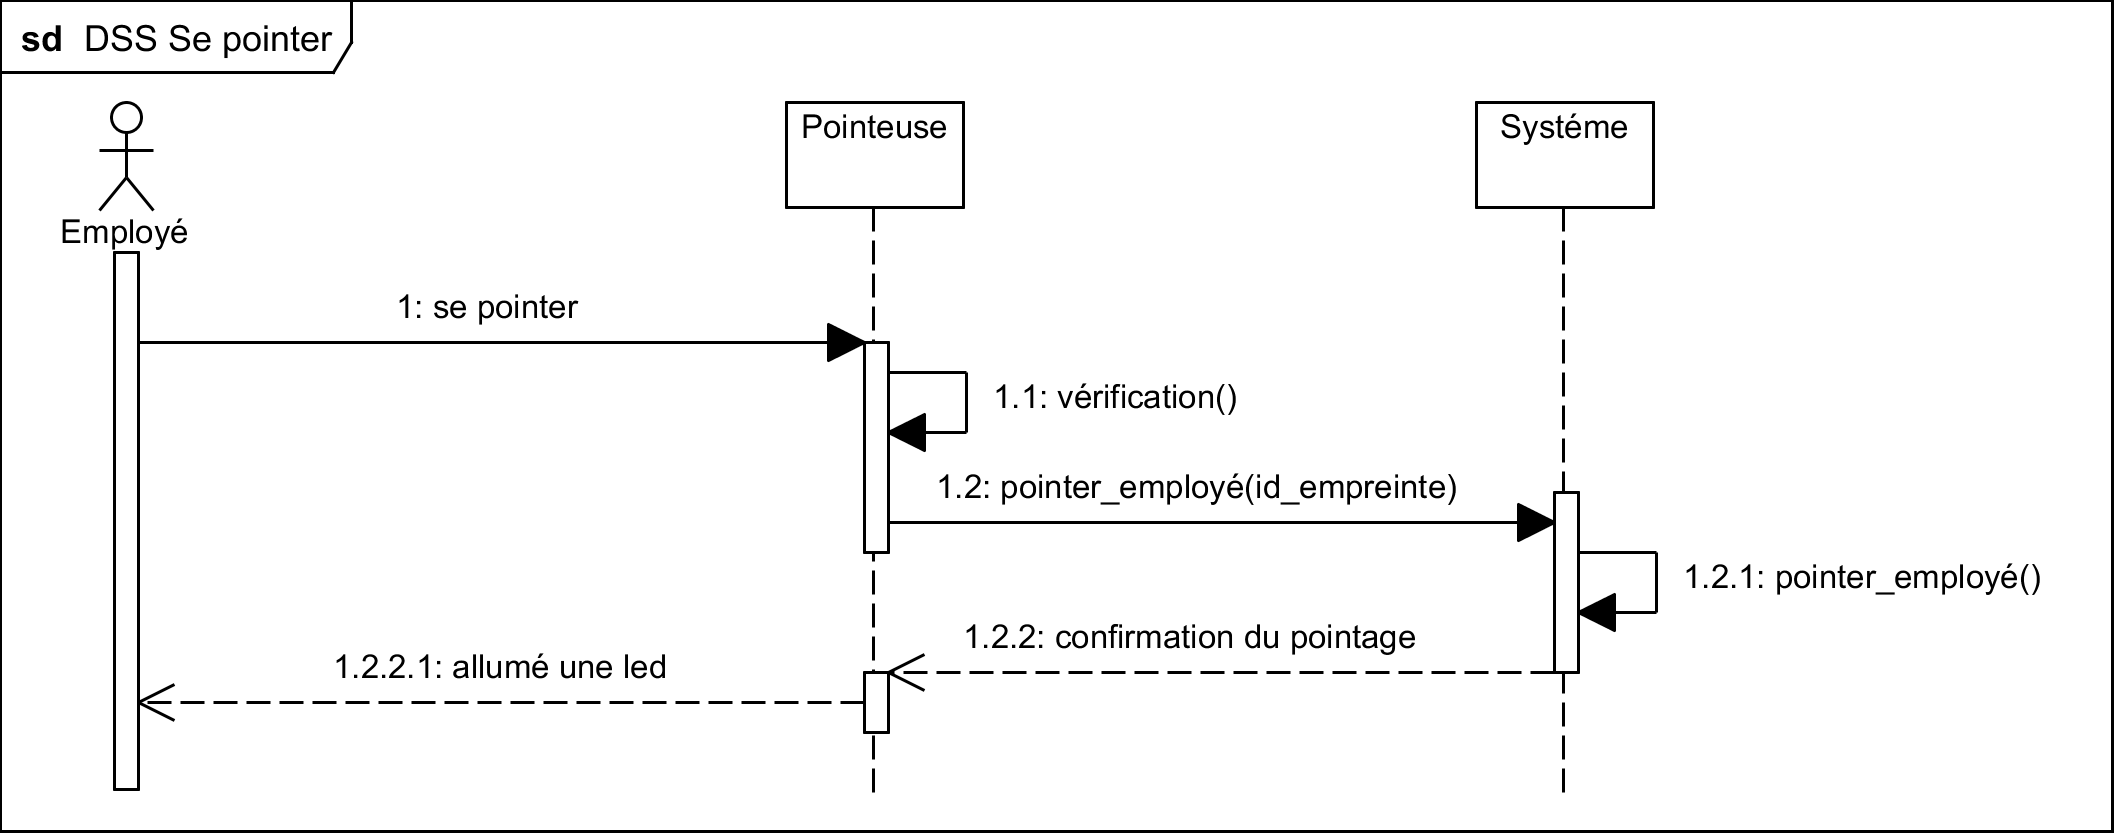
\includegraphics[scale=0.9]{images/DSS/DSS Se pointer.png}
         \caption{Diagramme de séquence système « Se pointer »}
         \label{fig4}
    \end{figure}
\vspace{-30pt}

\subsection{Cas d'utilisation « Consulter mon profil »}
L’employé peut décider de consulter son profil et avoir accès aux différentes
informations qui le concernent et modifier certaines valeurs s’il le souhaite, 
ou accéder à son planning. 
 
\begin{figure}[h!]
     \centering
     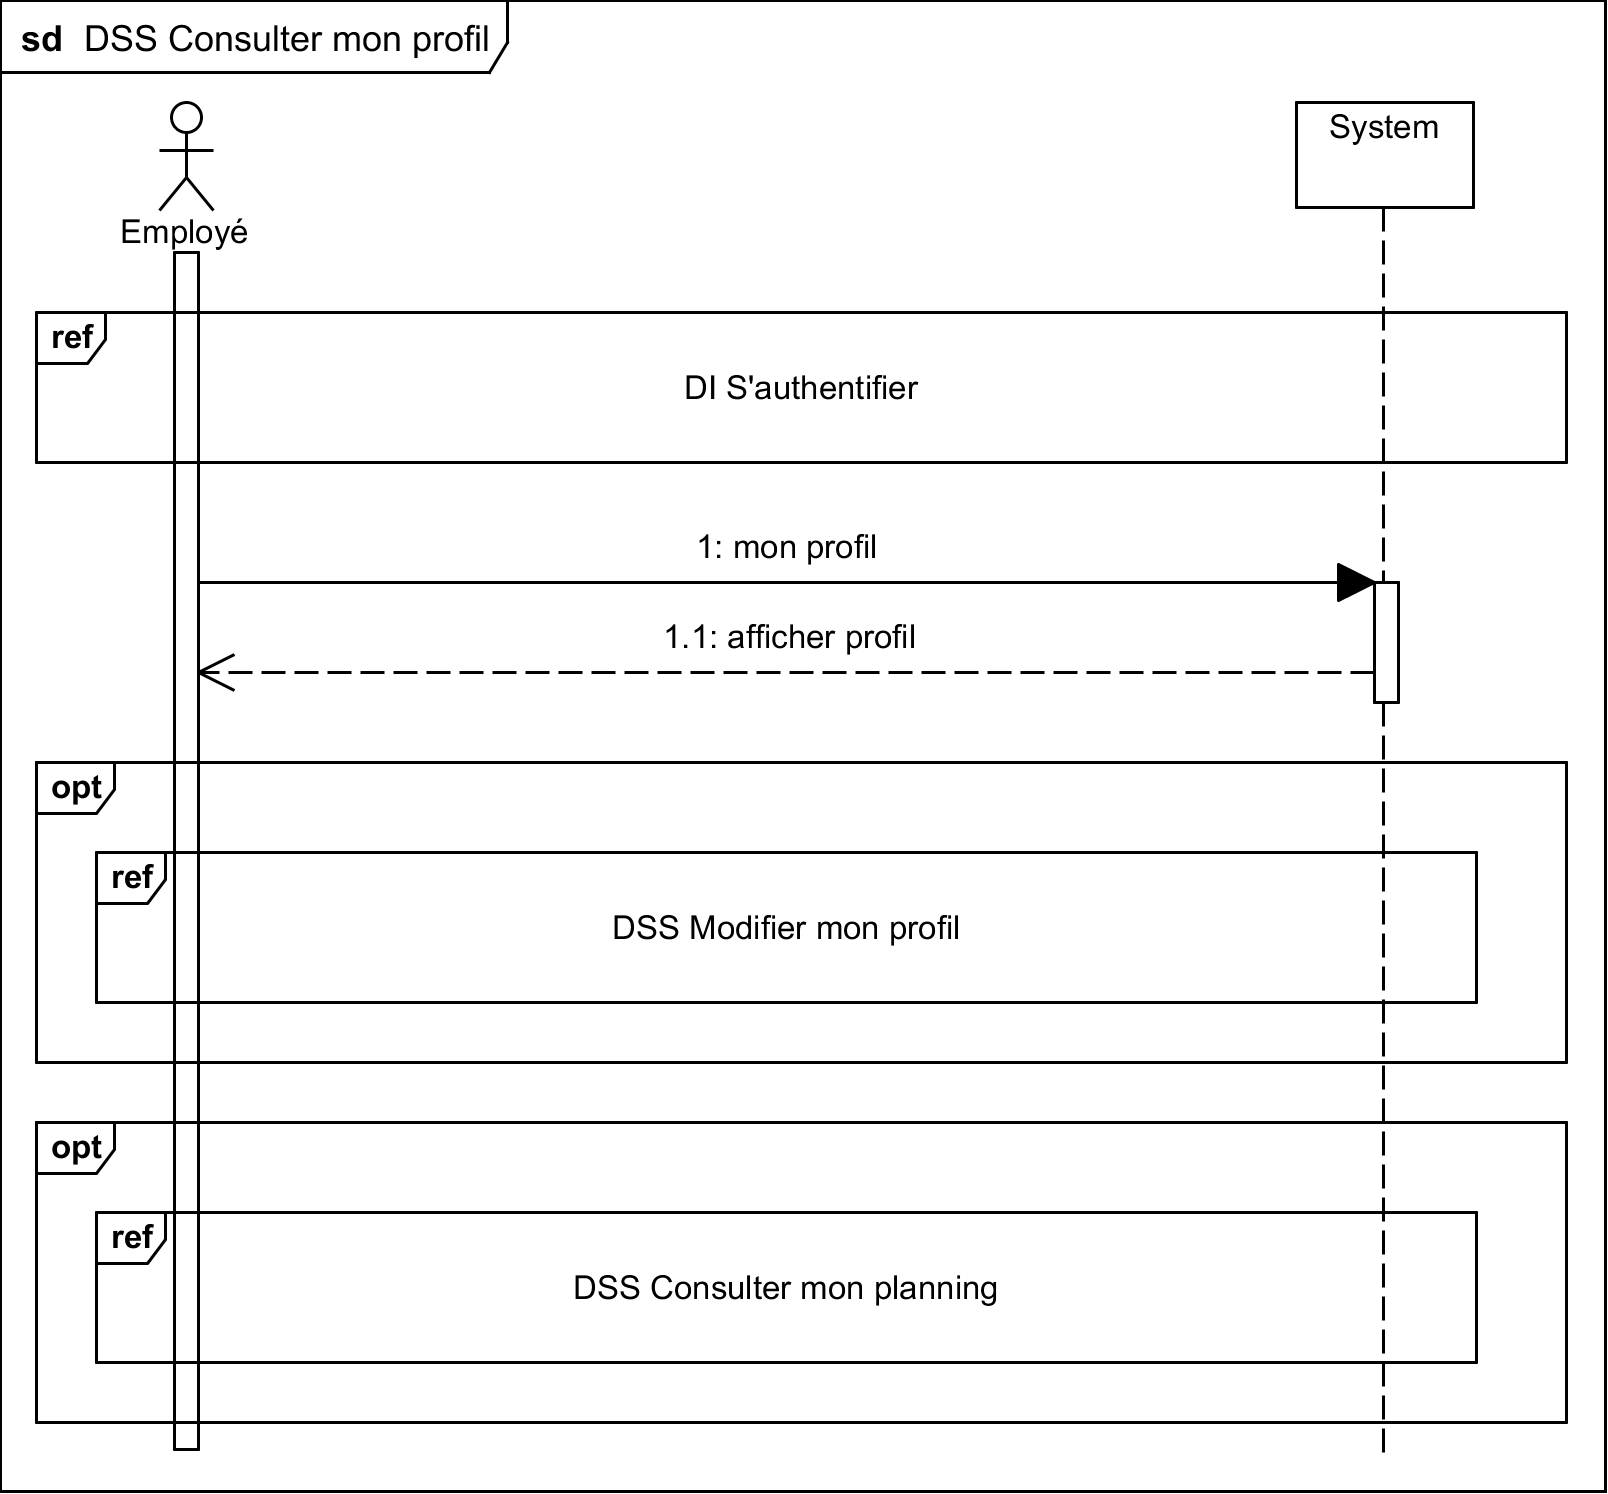
\includegraphics[scale=0.9]{images/DSS/DSS Consulter mon profil.png}
     \caption{Diagramme de séquence système « Consulter mon profil »}
     \label{fig4}
\end{figure}

\subsection{Cas d'utilisation « Consulter ma  fiche de pointage »}
Un employé peut consulter sa propre fiche de pointage qui comporte toutes les
informations concernant ses heures d’arrivée et de sortie des jours précédents.
Il peut aussi avoir a un affichage par semaine ou par mois.
   
\begin{figure}[h!]
     \centering
     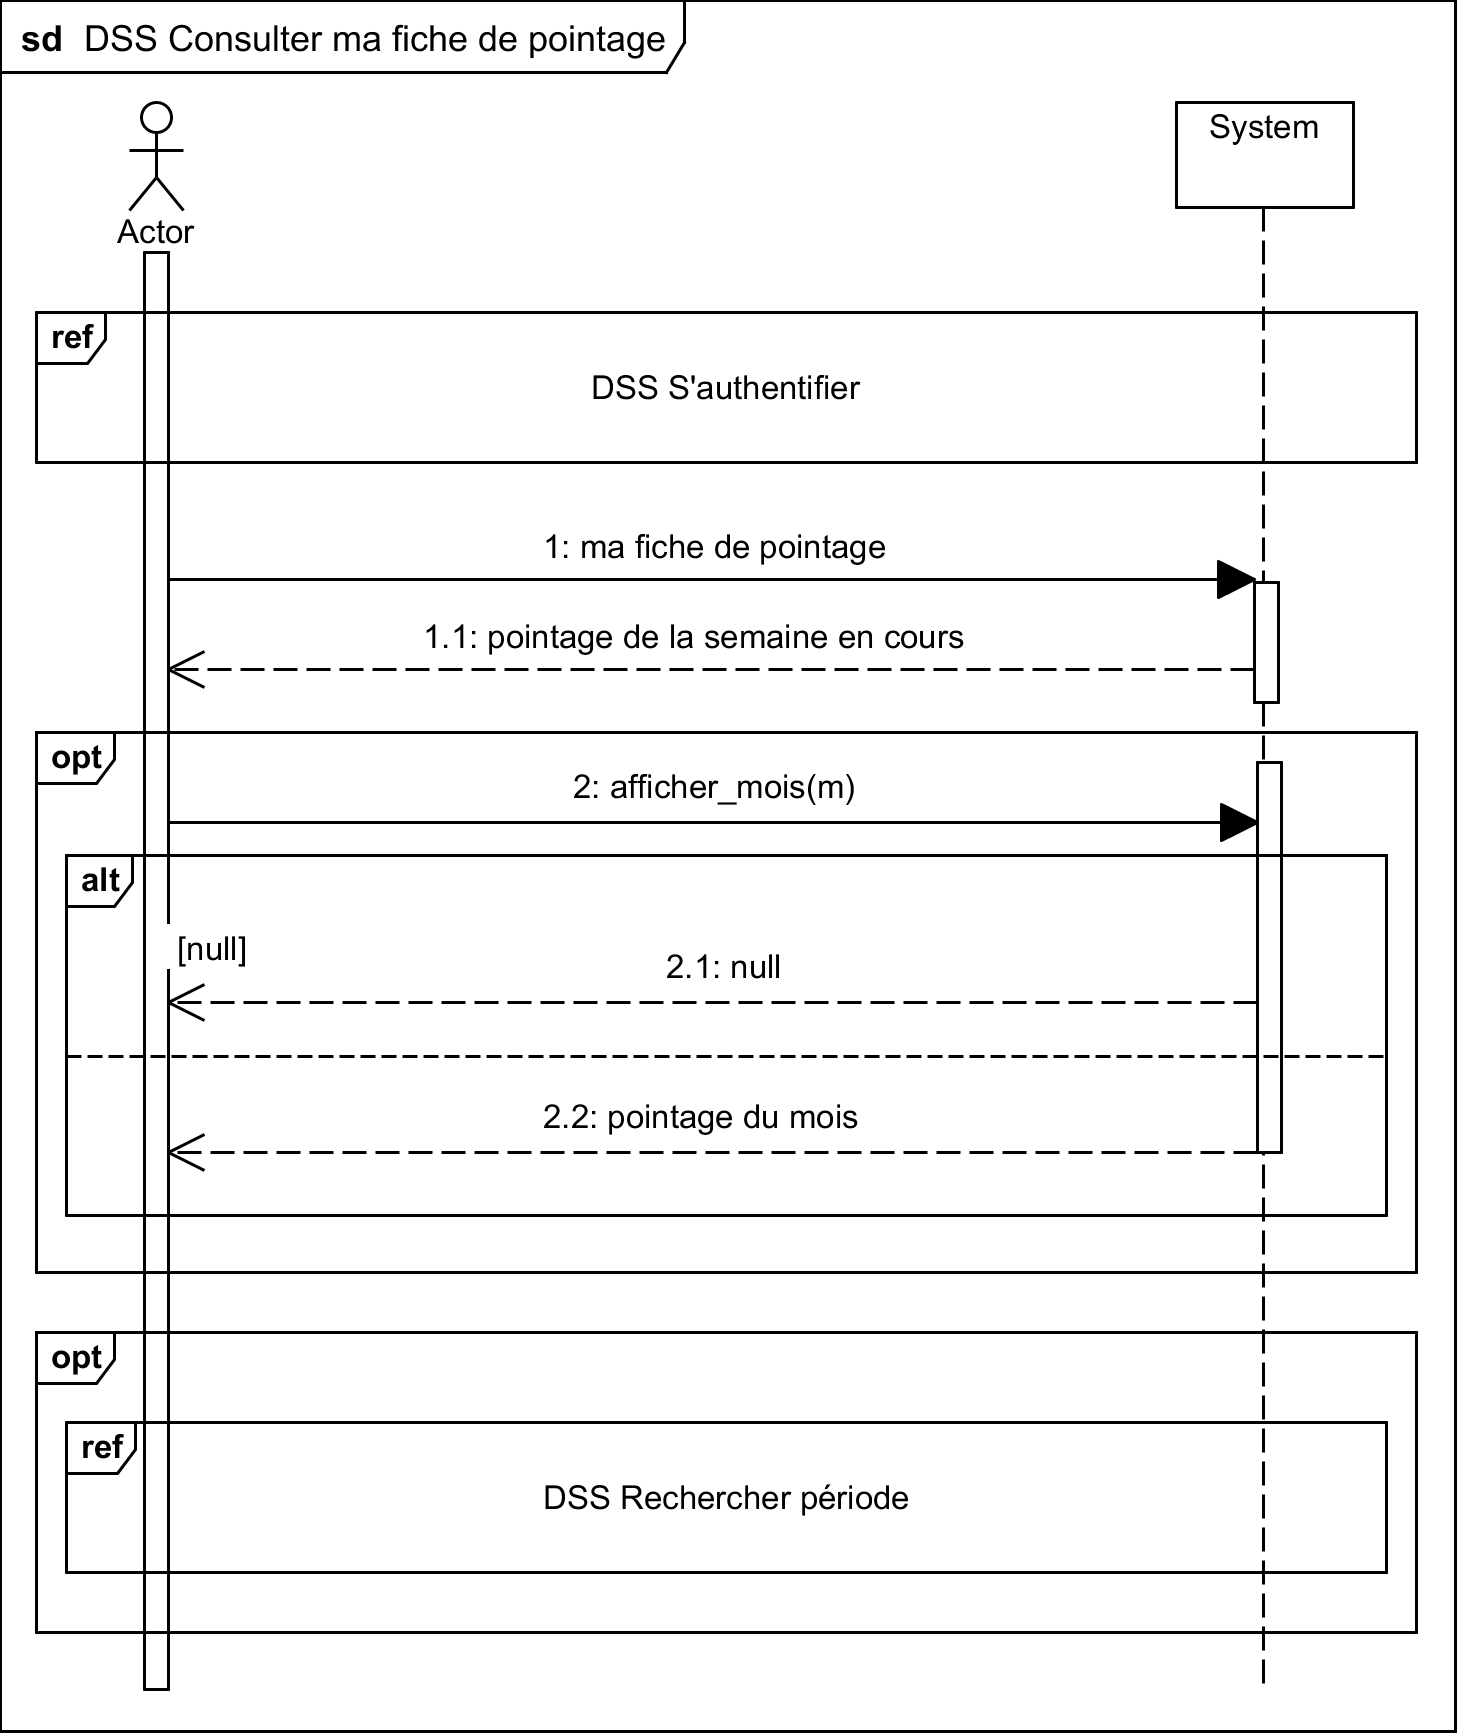
\includegraphics[scale=1.1]{images/DSS/DSS Consulter ma fiche de pointage.png}
     \caption{Diagramme de séquence système « Consulter ma  fiche de pointage »}
     \label{fig4}
\end{figure}

\vspace{-30pt}
\subsection{Cas d'utilisation « Consulter tableau de bord manager »}
Une fois authentifié, le manager sera redirigé directement vers son tableau de
bord qui est composé d’un espace en tant qu’employé et d'un autre consacré à ses
équipes. Grâce auquel il aura un récapitulatif de présence de ses
collaborateurs, leurs nombres, ainsi que leur dernier pointage et le temps passé
en poste.

\begin{figure}[h!]
     \centering
    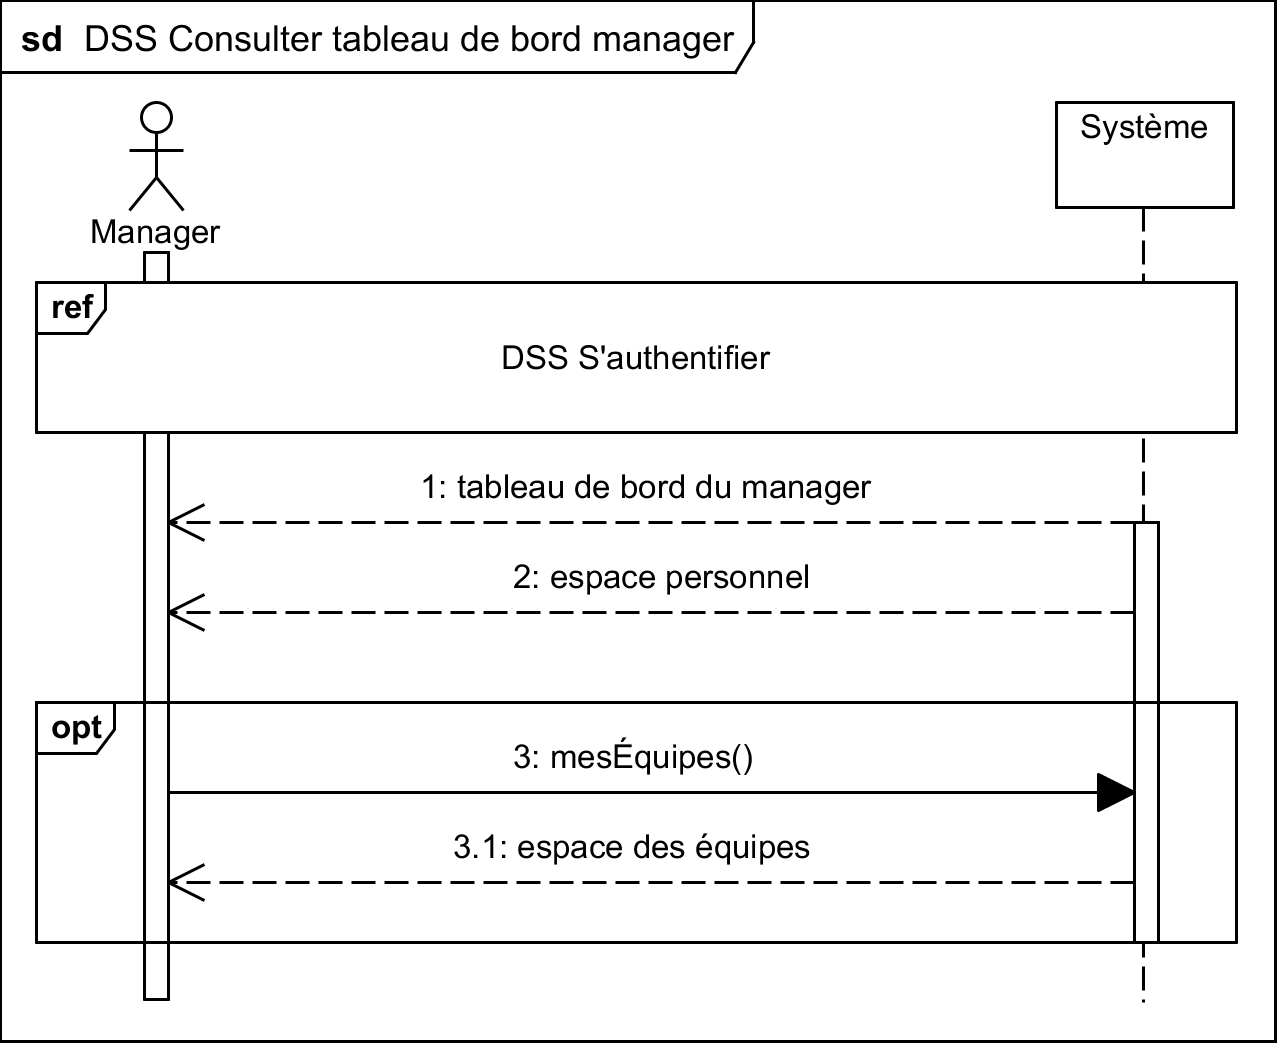
\includegraphics[scale=1]{images/DSS/DSS Consulter tableau de bord manager.png}
     \caption{Diagramme de séquence système « Consulter tableau de bord manager »}
     \label{fig4}
\end{figure}

\vspace{-30pt}
\subsection{Cas d'utilisation « Ajouter membre »}
Un responsable décide d’ajouter un membre à une équipe, il commence par
sélectionner l’équipe puis il effectue une recherche pour trouver l’employé pour
enfin l’ajouter en tant que membre de cette dernière.  

\begin{figure}[h!]
     \centering
    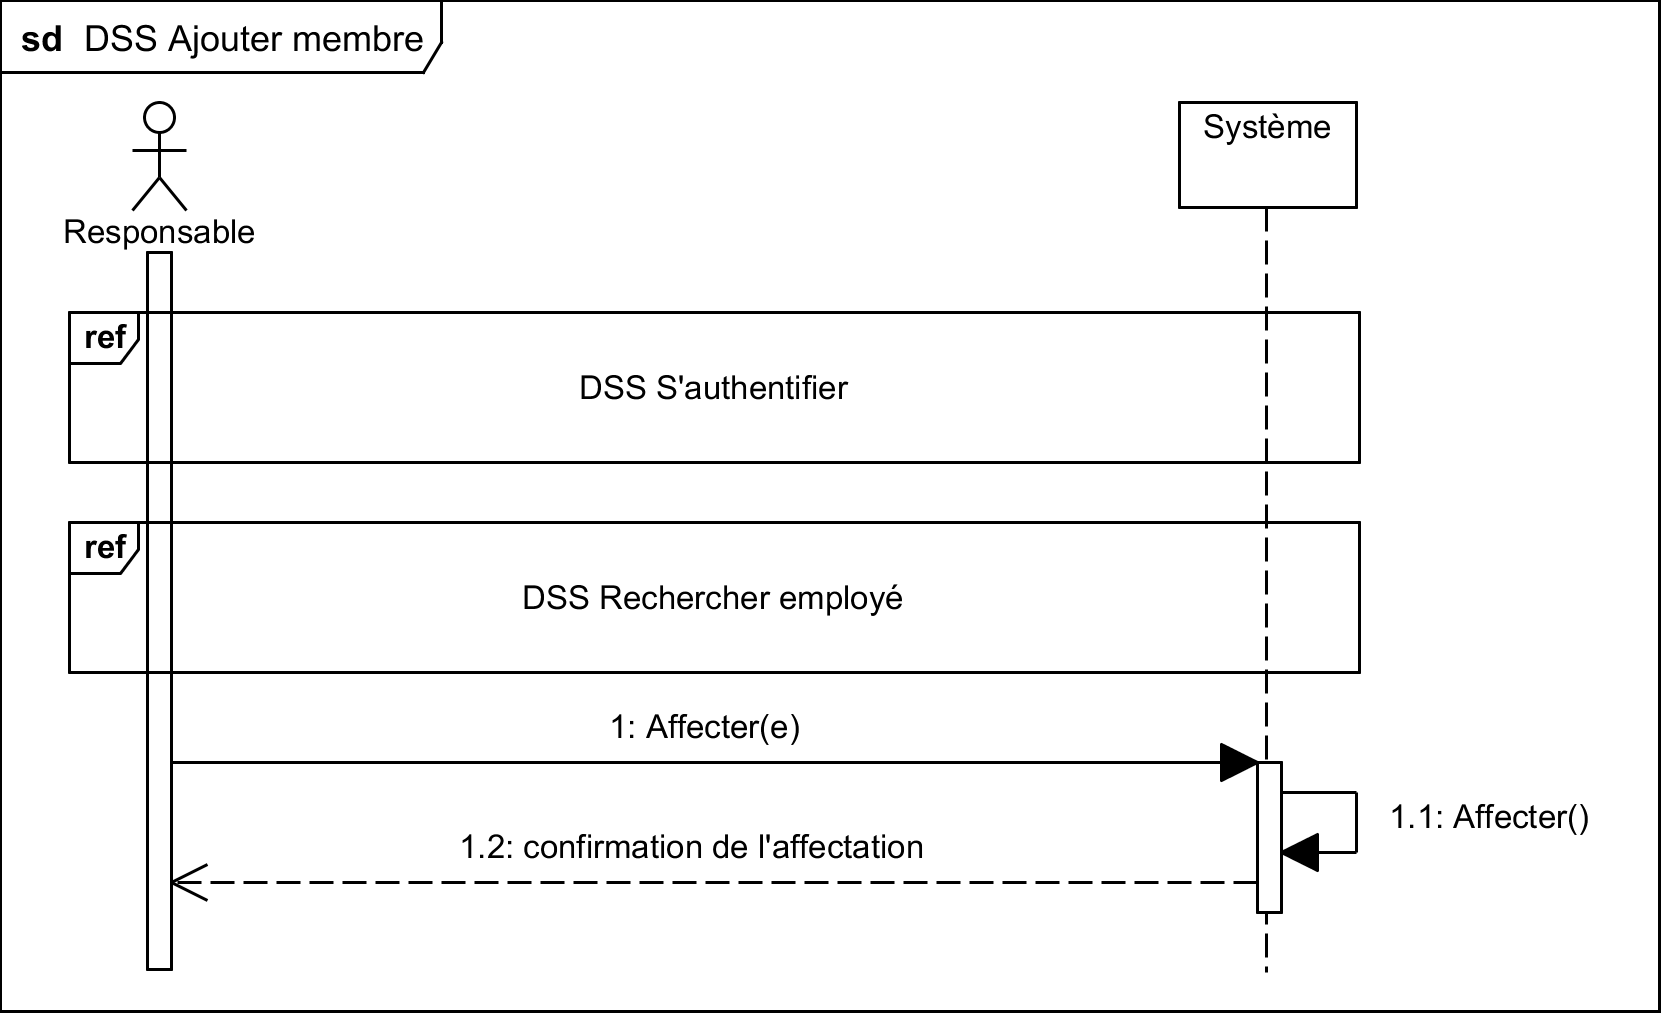
\includegraphics[scale=1]{images/DSS/DSS Ajouter membre.png}
     \caption{Diagramme de séquence système « Ajouter membre »}
     \label{fig4}
\end{figure}
    
\subsection{Cas d'utilisation « Ajouter planning »}
Un responsable peut créer un planning d’une semaine où il définit les jours de
travail ainsi que les horaires pour chaque jour. Pour ce, il doit saisir un
intitulé pour le planning et une description ainsi que les horaires d’entrée et
de sortie.   

\begin{figure}[h!]
     \centering
    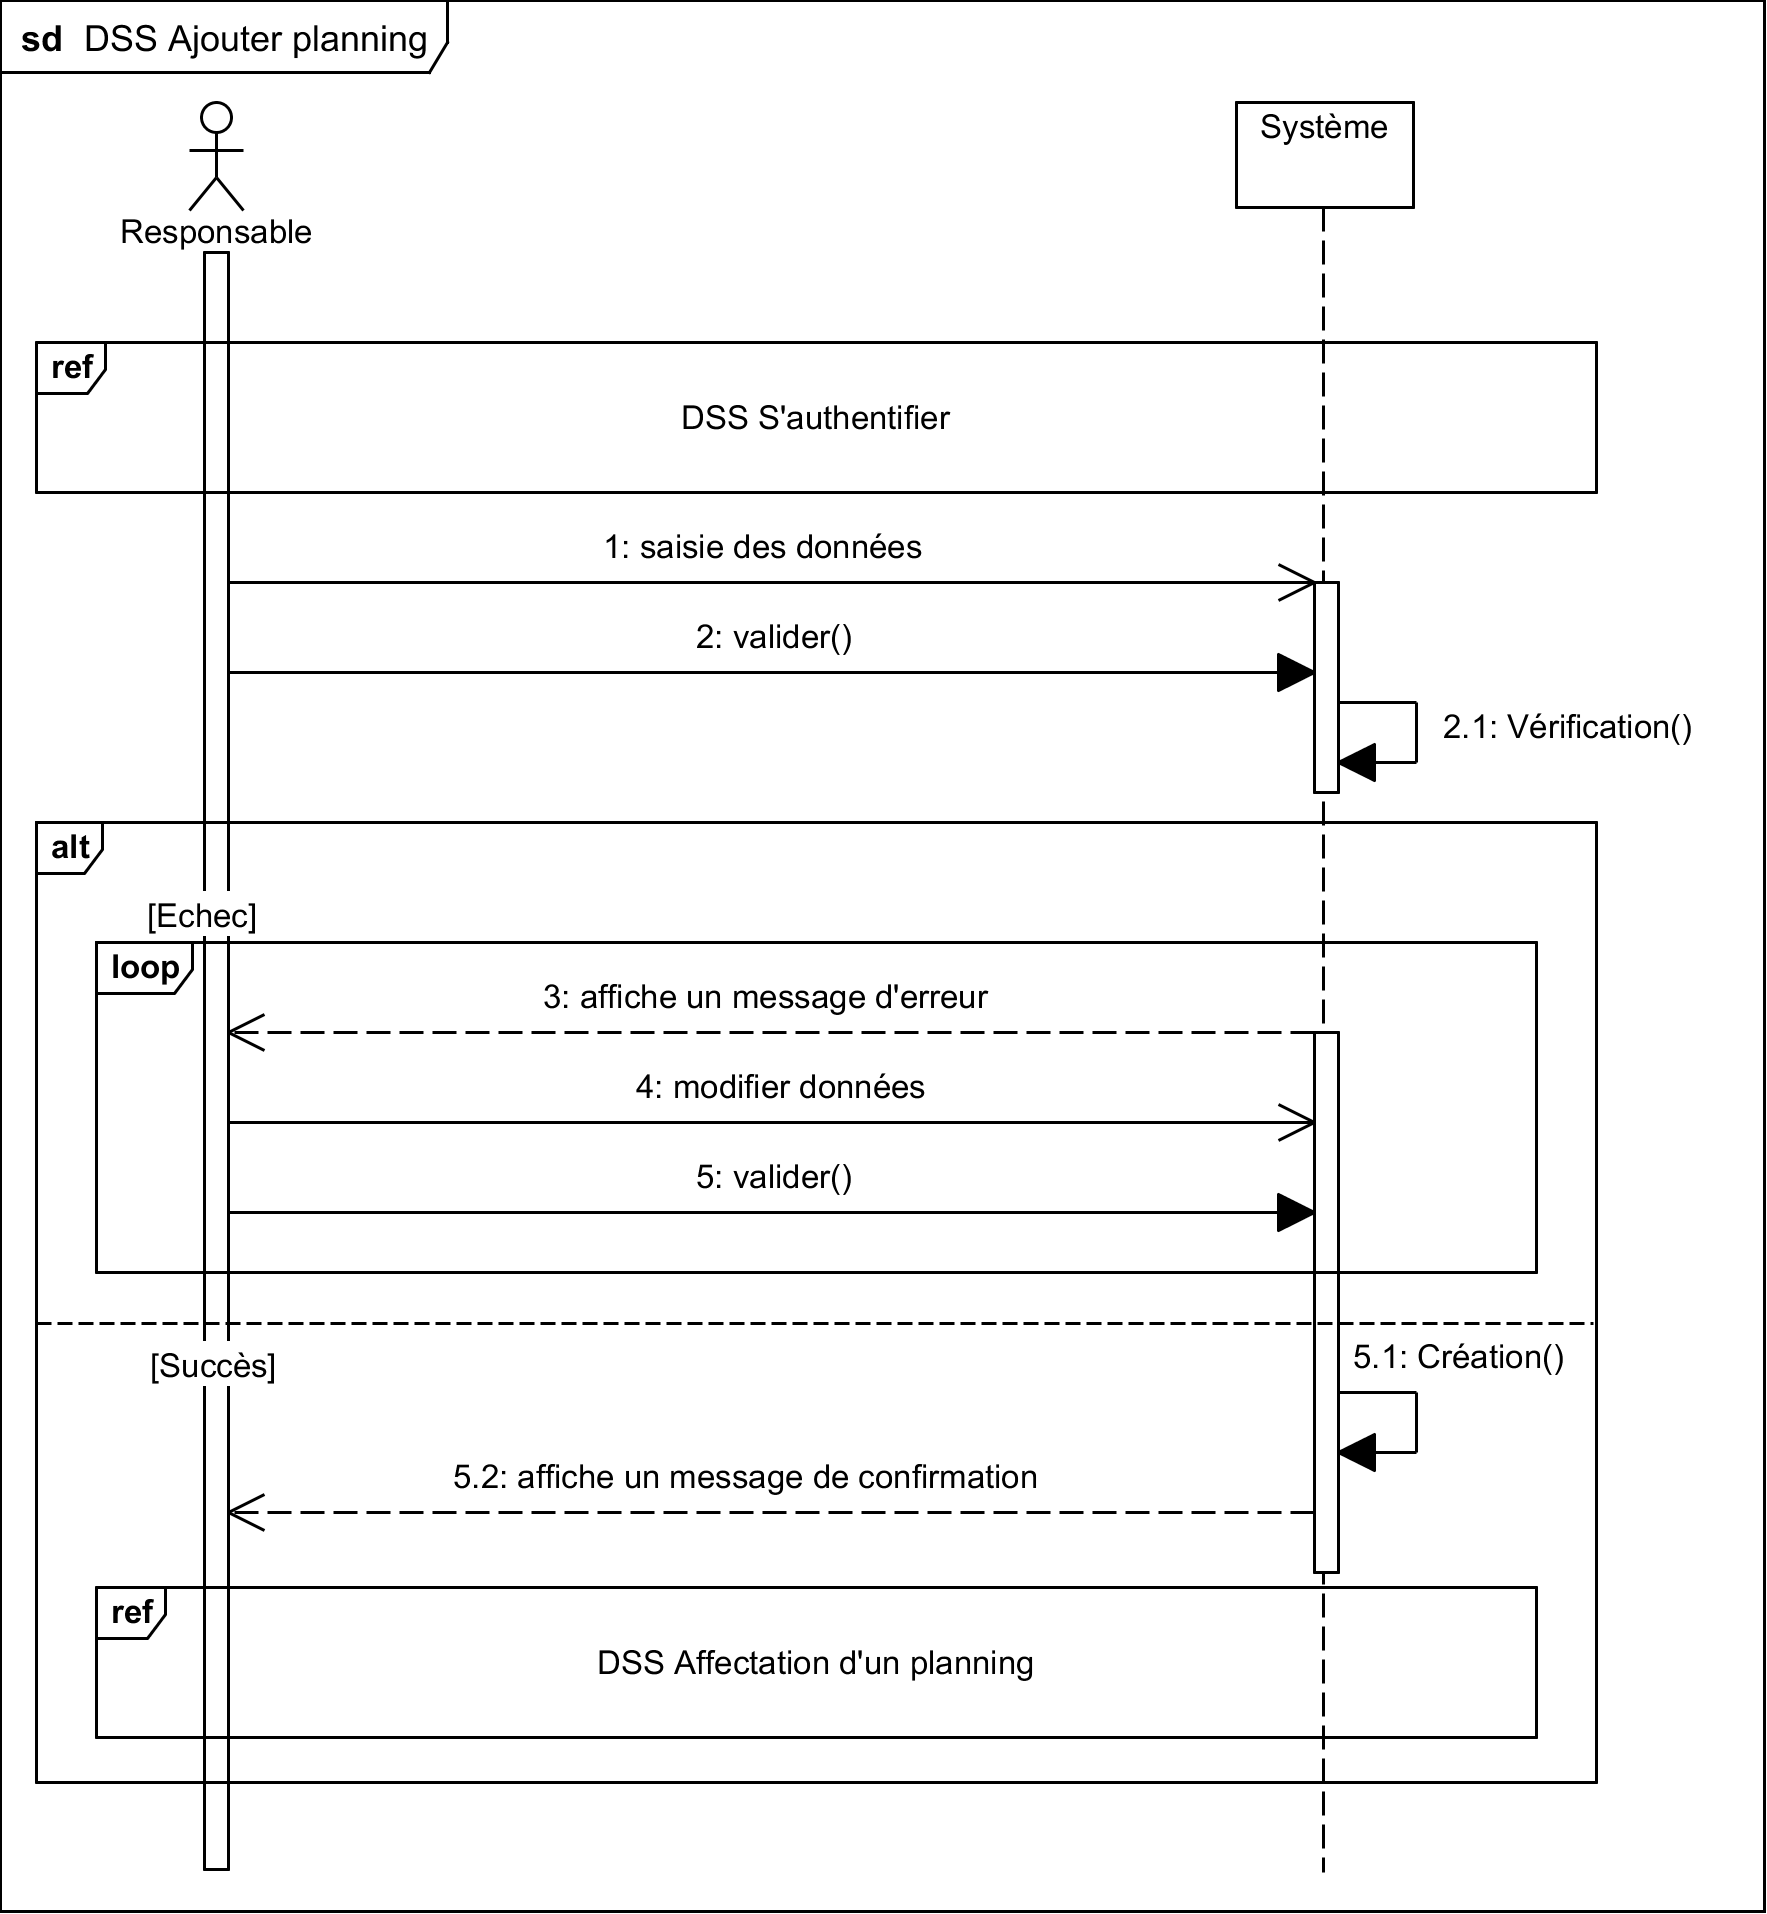
\includegraphics[scale=1]{images/DSS/DSS Ajouter planning.png}
     \caption{Diagramme de séquence système « Ajouter planning »}
     \label{fig4}
\end{figure}
    
\subsection{Cas d'utilisation « Ajouter équipe »}
Pour créer une équipe, le responsable doit saisir l’intitulé et la description
de l’équipe puis lui attribuer un manager. Une fois l’équipe créée, il pourra
ajouter des membres à cette équipe.   

\clearpage
\begin{figure}[h!]
     \centering
    \includegraphics[scale=1]{images/DSS/DSS Ajouter une équipe.png}
     \caption{Diagramme de séquence système « Ajouter équipe »}
     \label{fig4}
\end{figure}
    
\subsection{Cas d'utilisation « Ajouter employé »}
Un responsable peut créer un employé, il doit saisir les informations le
concernant. Une fois l’employé crée, il doit ajouter son empreinte.   

\clearpage
\begin{figure}[h!]
     \centering
    \includegraphics[scale=1.1]{images/DSS/DSS Ajouter employé.png}
     \caption{Diagramme de séquence système « Ajouter employé »}
     \label{fig4}
\end{figure}

\subsection{Cas d'utilisation « Consulter le profil d'un employé »}
Le responsable peut consulter le profil d’un employé qui contient les
informations de ce dernier. Il aura aussi la possibilité de le modifier ainsi
que de consulter son planning.

\clearpage
\begin{figure}[h!]
     \centering
    \includegraphics[scale=1]{images/DSS/DSS Consulter profil d'un employé.png}
     \caption{Diagramme de séquence système « Consulter profil d'un employé »}
     \label{fig4}
\end{figure}

Dans un souci de lisibilité, nous avons déplacé le reste des diagrammes de
séquence système vers l’annexe B \ref{ch:annexeB}.  
    
\section{Les maquettes IHM }
    
\subsection{Employé}
La figure \ref{fig6} : Une fois, authentifié, cette interface sera la première
affichée à l’utilisateur ayant le rôle d’un employé. On remarque un menu sur le
côté gauche, un composant qui sera présent sur la totalité des interfaces du
projet, et qui permet une navigation entre les différentes fonctionnalités
qu’offre le système tout en s’adaptant au rôle de l’utilisateur connecté.
L’utilisateur peut à tout moment se déconnecter grâce au bouton présent au bas
du menu.

Cette interface représente le tableau de bord de l’employé, elle regroupe les
informations les plus récentes et les plus pertinentes, comme ses horaires du
jour ou son dernier pointage ainsi que le temps passé en poste. Une seconde
partie est dédiée à des informations concernant ses collaborateurs faisant
partie de son équipe.
        
La figure \ref{fig7} : représente l’affichage du profil de l’employé lui-même,
où ses informations sont regroupées en catégories selon leurs utilité et leurs
importance. Il existe un bouton qui permet à l’employé de visualiser son
planning à partir de cette interface directement. 

\clearpage
        
\begin{figure}[h!]
    \centering
    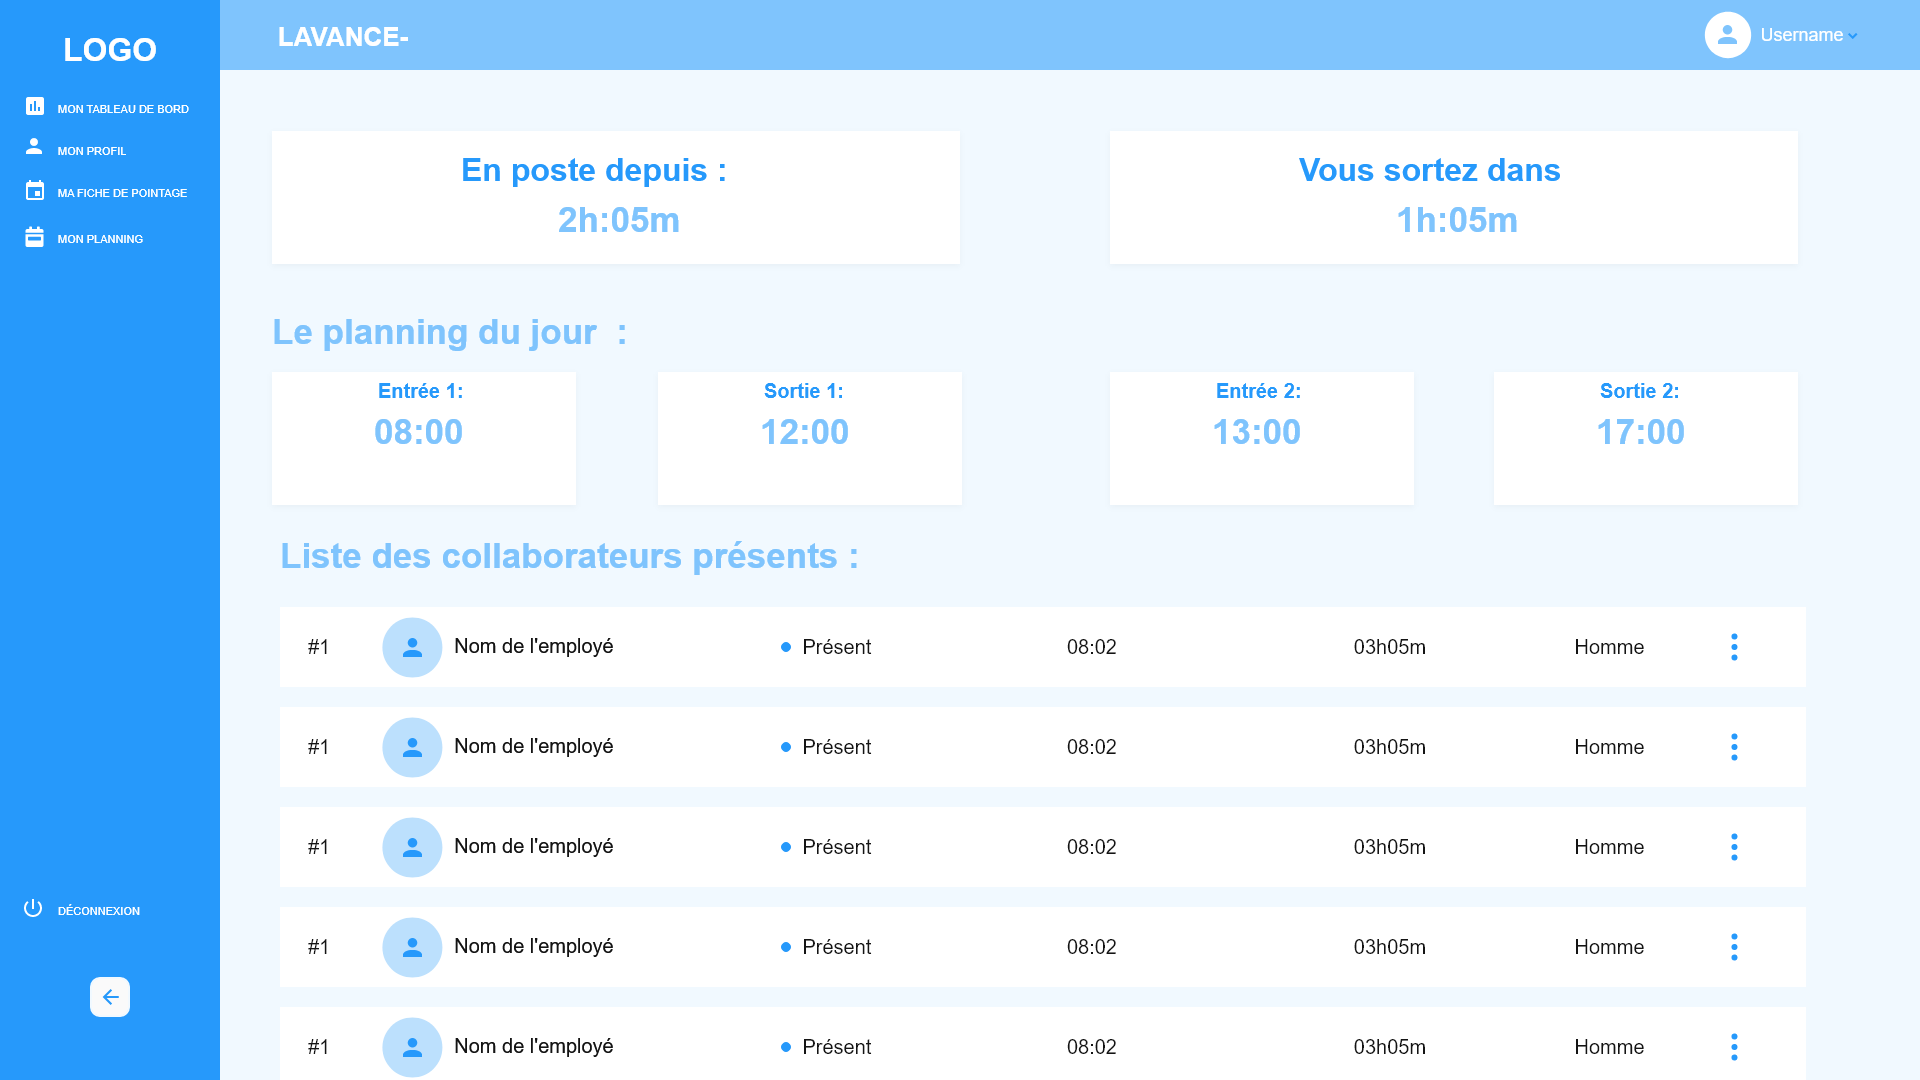
\includegraphics[width=18cm]{images/dash_emp.png}
    \caption{Maquette tableau de bord Employé}
    \label{fig6}
\end{figure}

\begin{figure}[h!]
    \centering
    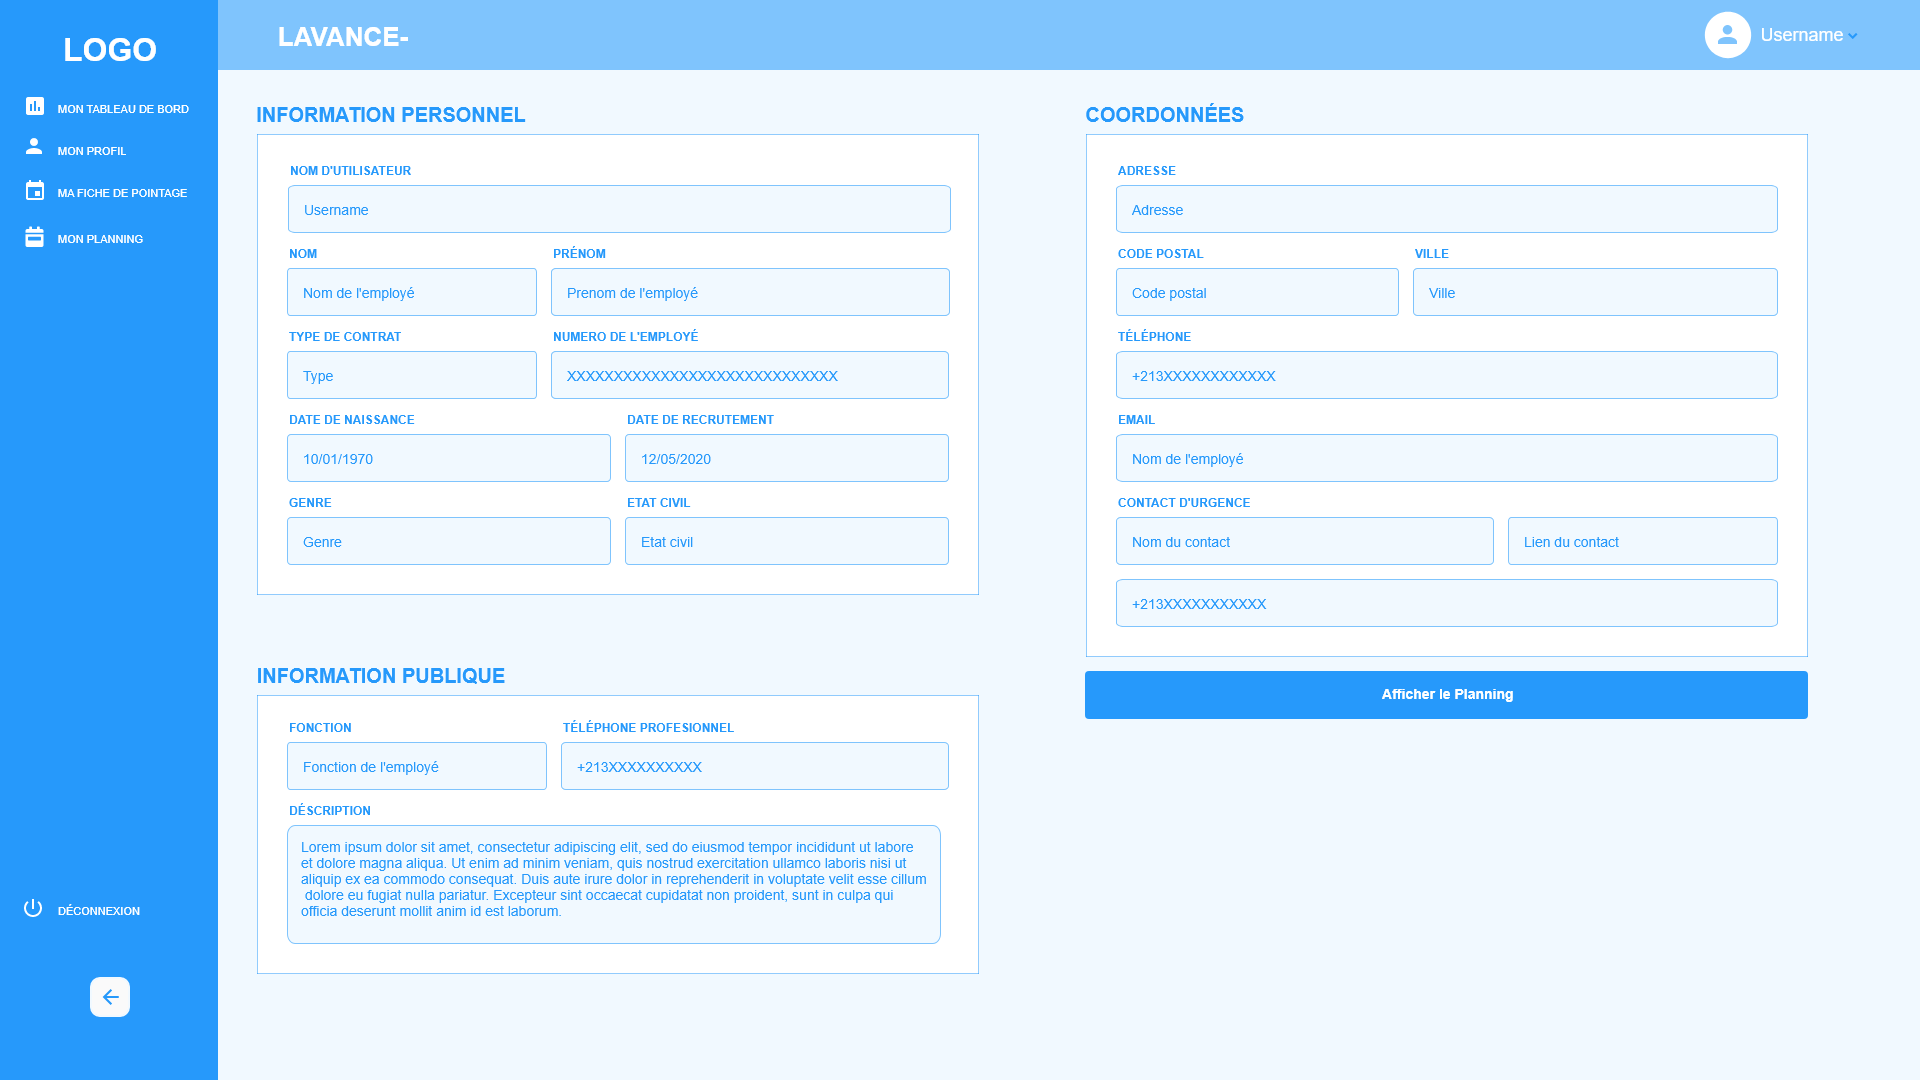
\includegraphics[width=18cm]{images/profil.png}
    \caption{Maquette profil Employé}
    \label{fig7}    
\end{figure}
        
\subsection{Manager}
La figure \ref{fig8} : ici, on représente le tableau de bord du manager qui est
composé de deux onglets. Le premier onglet est identique au tableau de bord de
l’employé simple, tandis que l’onglet « Mes équipes » récapitule l’ensemble des
informations concernant les équipes sous la responsabilité d’un manager. Il met
en évidence le nombre total des équipes et des collaborateurs, le récapitulatif
de présence de ces derniers sous forme de graphe, ainsi qu’une liste des
employés avec leurs derniers pointages
        
La figure \ref{fig9} : cette interface affiche les informations qui concernent
une équipe sélectionnée au préalable par le manager. On peut y voir le titre, la
description de l’équipe ainsi que des statistiques. Dans la partie inférieure,
on liste l’ensemble des employés appartenant à cette équipe avec la possibilité
d’un accès direct vers le profil de chacun d’eux.

\begin{figure}[h!]
    \centering
    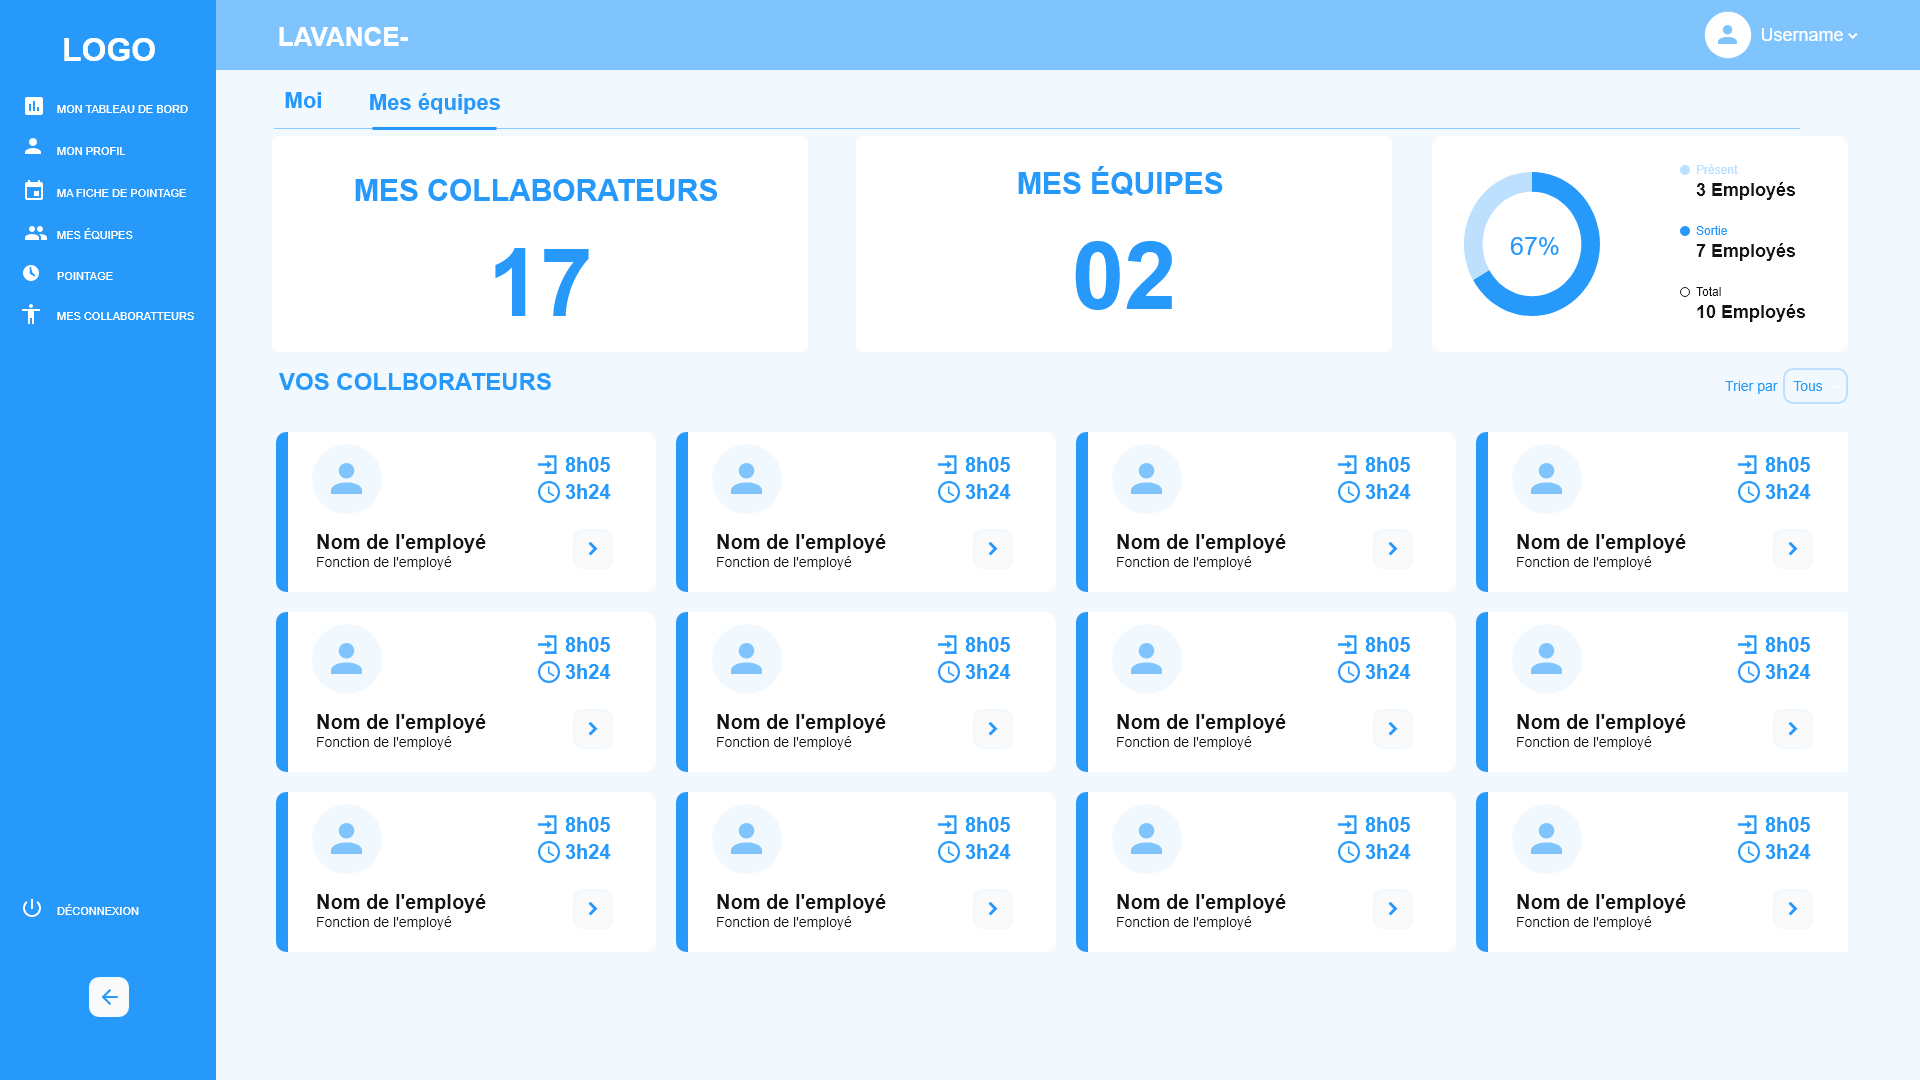
\includegraphics[width=18cm]{images/dash_man_my_teams.png}
    \caption{Maquette tableau de bord Manager}
    \label{fig8}
\end{figure}

\clearpage

\begin{figure}[h!]
    \centering
    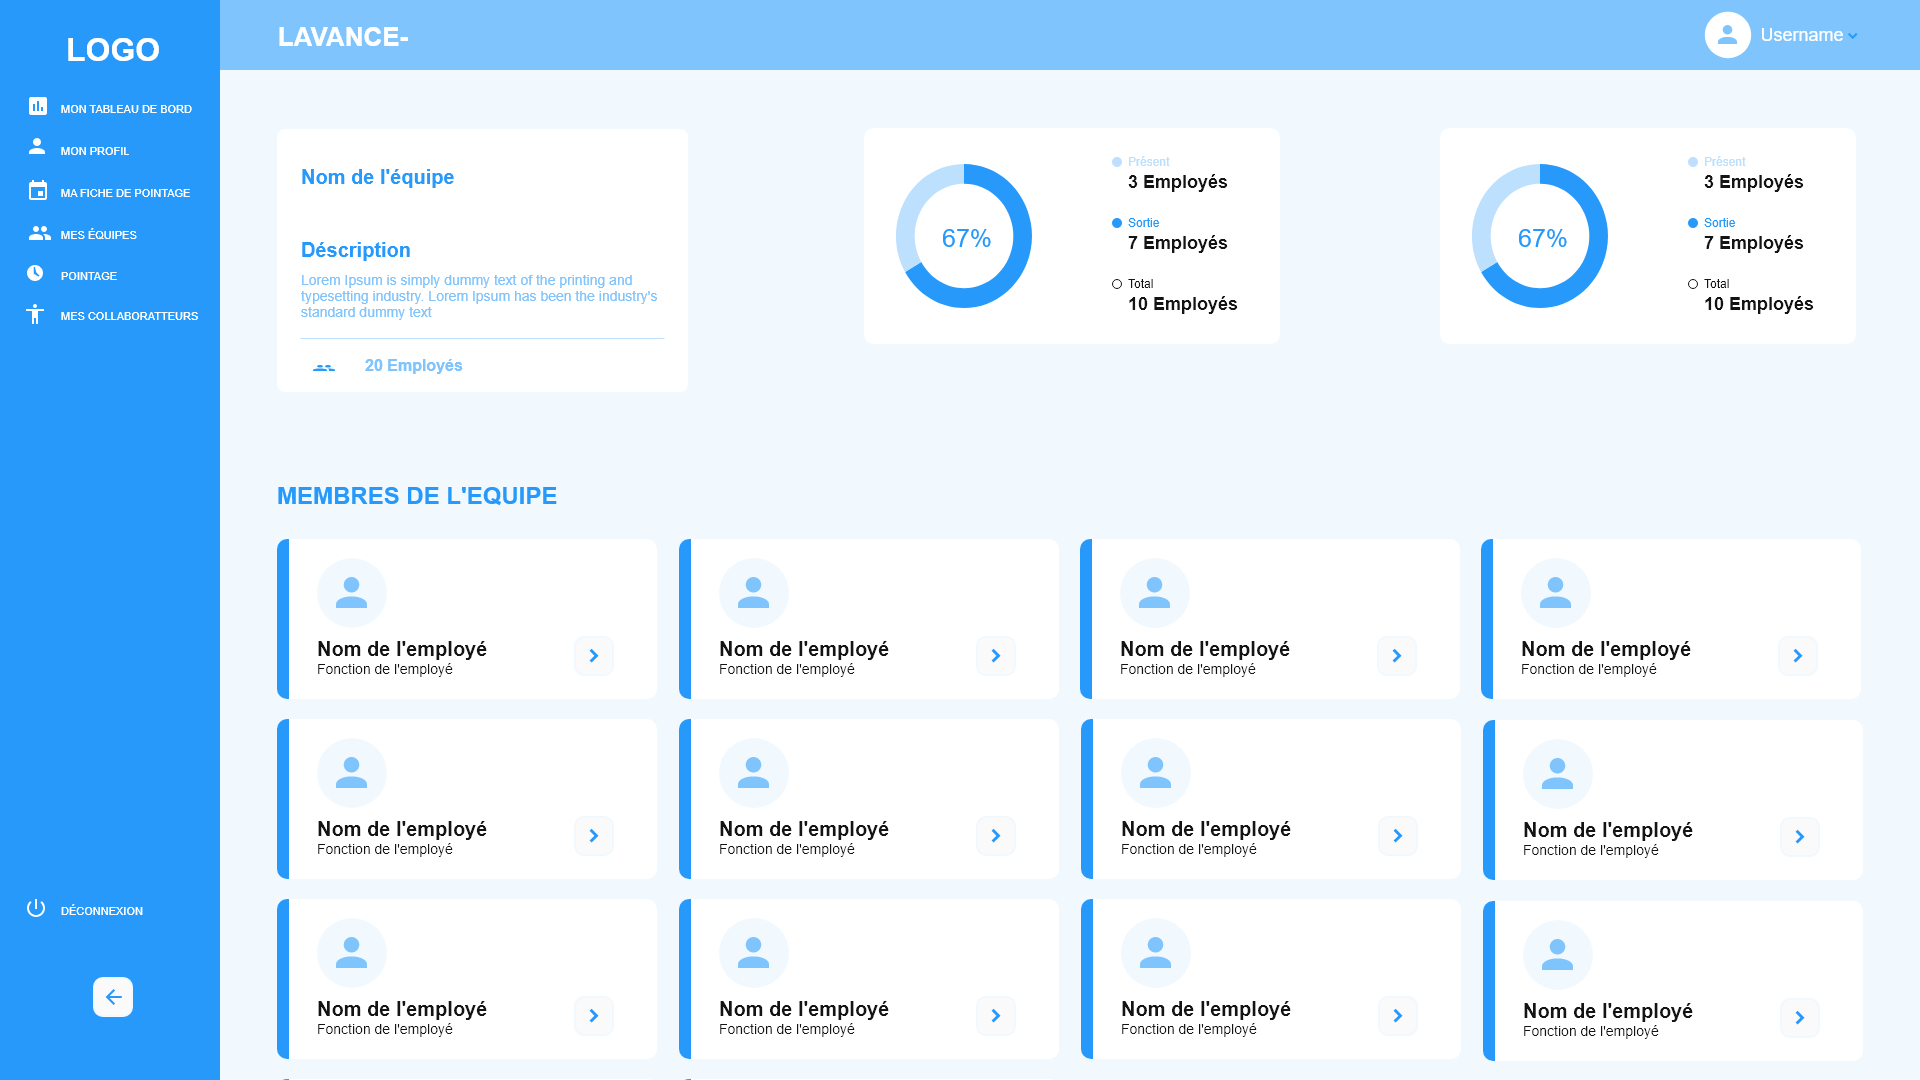
\includegraphics[width=18cm]{images/my_team.png}
    \caption{Maquette les équipes d'un Manager}
    \label{fig9}
\end{figure}


\subsection{Responsable}
La figure \ref{fig10} : représente l’interface dans laquelle le responsable crée
un planning en lui attribuant un nom et une description et les horaires de début
et de fin des périodes de travail tout au long de la semaine, avec chaque jour
étant composé de deux parties.
 
La figure \ref{fig11} : représente l’interface avec laquelle un responsable
affecte un planning à un ou des employés en effectuant une recherche par lettre
qui affiche une liste des employés ayant un nom ou un prénom correspondant aux
caractères saisis, et un bouton qui permet d’affecter l’employé sélectionné.
L’interface comporte aussi une liste des employés ayant déjà été affectés à ce
planning avec la possibilité de détacher un employé du planning. 

\clearpage

\begin{figure}[h!]
    \centering
    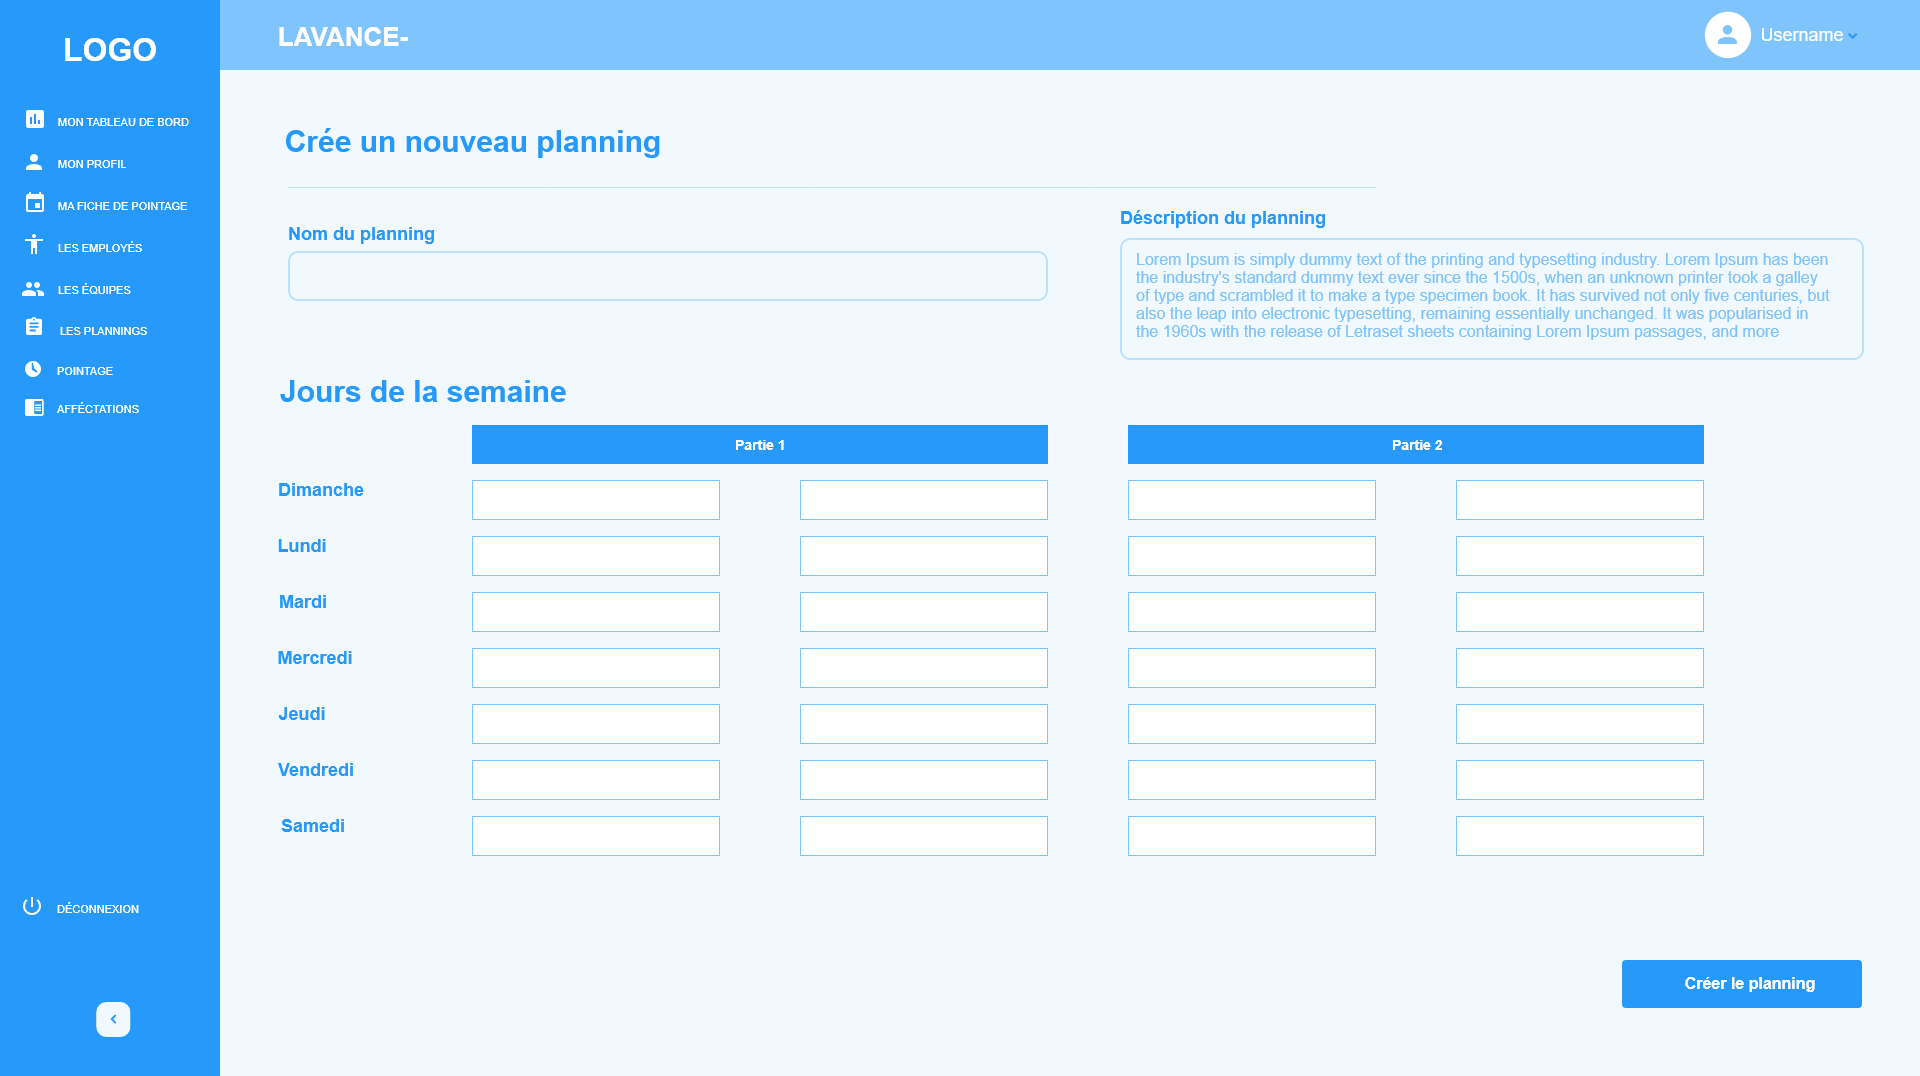
\includegraphics[width=18cm]{images/add_panning.png}
    \caption{Maquette création d'un planning}
    \label{fig10}
\end{figure}



\begin{figure}[h!]
    \centering
    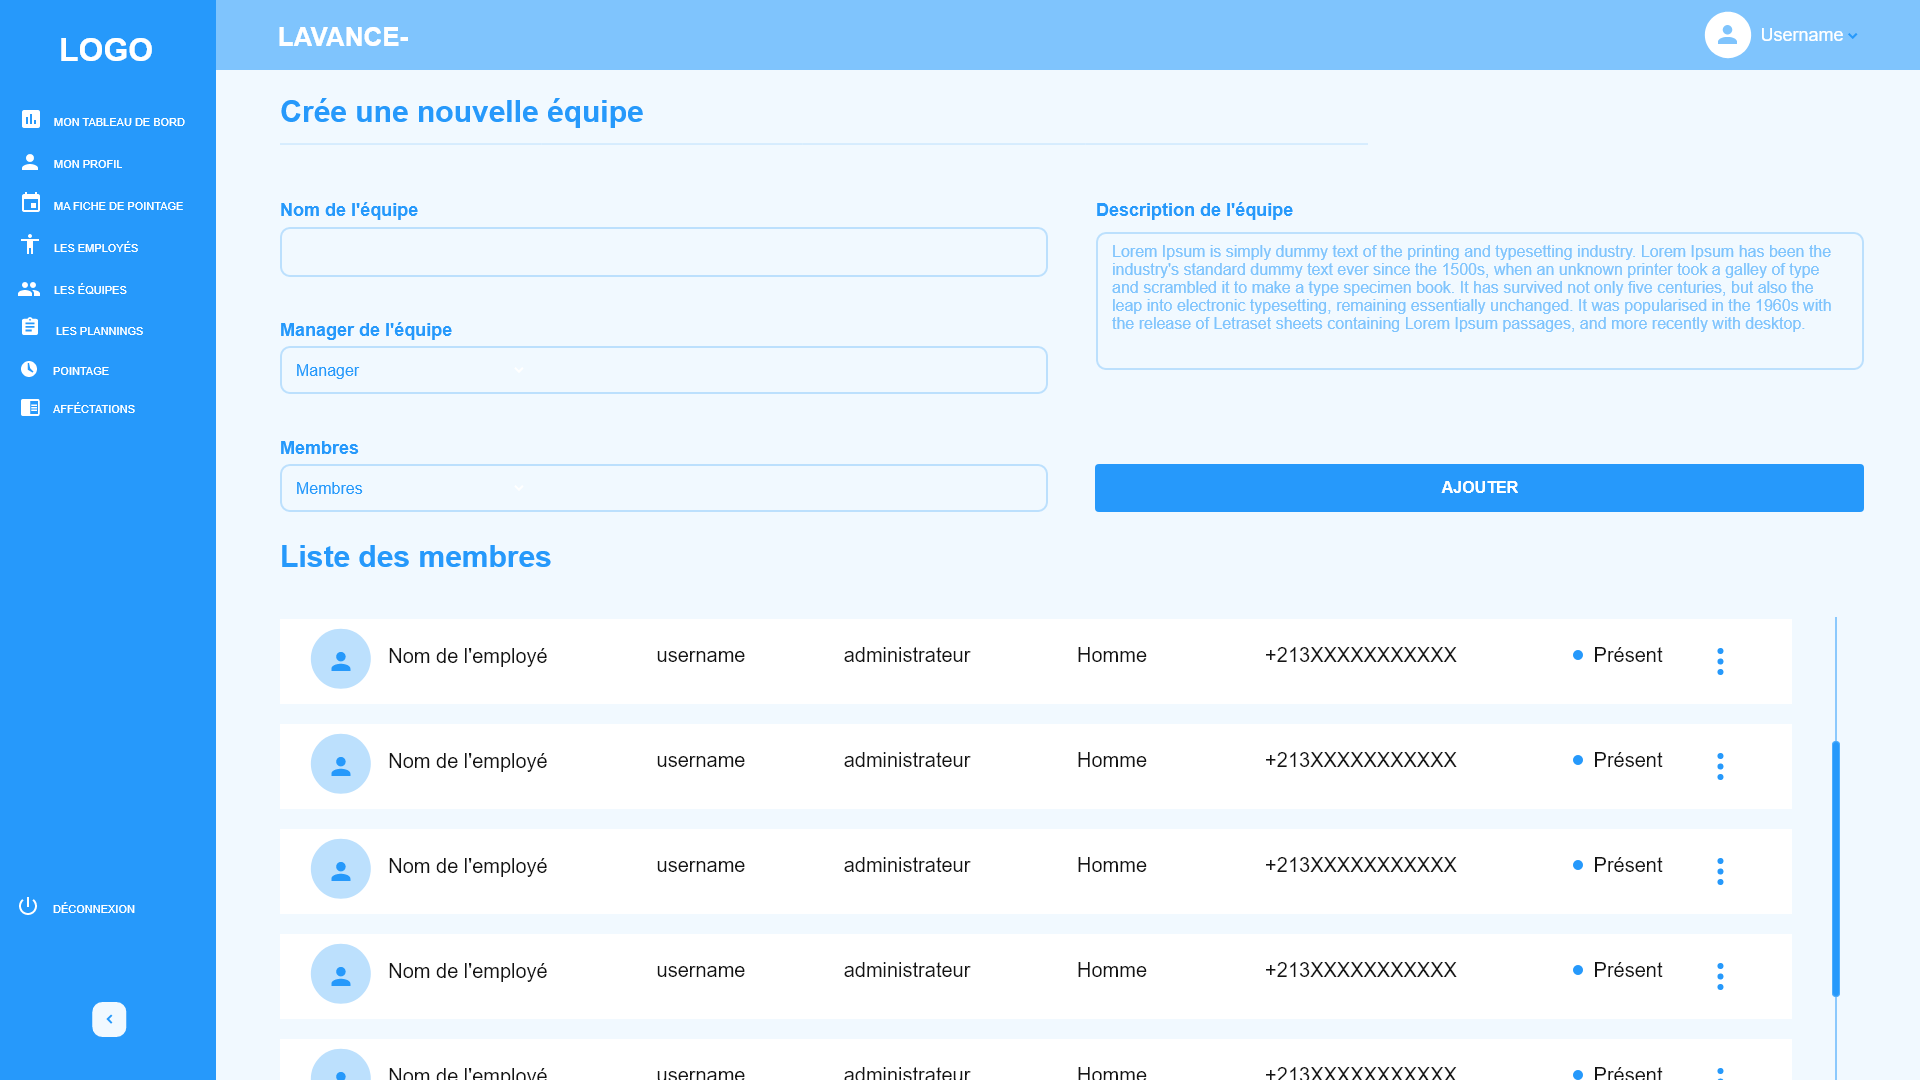
\includegraphics[width=18cm]{images/add_member.png}
    \caption{Maquette affectations d'un employé a une équipe }
    \label{fig11}
\end{figure}

\clearpage
À travers ces quelques maquettes, nous avons essayé de vous transmettre notre
vision générale du projet sur son aspect graphique, et la composition globale de
certaines interfaces. Le reste des maquettes sera présenté de manière détaillée
dans l’annexe.
        
\subsection{la navigation}
L’outil utilisé pour réaliser les maquettes offre la possibilité de créer un
prototype complet et très représentatif du résultat final. Ci-dessous, des liens
vers les prototypes réalisés comportant toutes les interfaces et les liens de
navigations.\\

Prototype employé: \href{https://xd.adobe.com/view/9afd474c-7053-4831-4a92-bb9d2f4d8c65-eccc/?fullscreen&hints=off}{lien du prototype 1}
URL :<https://xd.adobe.com/view/9afd474c-7053-4831-4a92-bb9d2f4d8c65-eccc/?fullscreen&hints=off>\\
Prototype manager: \href{https://xd.adobe.com/view/855f8afc-8c35-451d-7b50-838460e72c7e-f36e/?fullscreen&hints=off}{lien du prototype 2}
URL :<https://xd.adobe.com/view/855f8afc-8c35-451d-7b50-838460e72c7e-f36e/?fullscreen&hints=off>\\
Prototype responsable: \href{https://xd.adobe.com/view/8c62407e-81ae-4950-60f2-88006b652695-fa53/?fullscreen&hints=off}{lien du prototype 3}
URL :<https://xd.adobe.com/view/8c62407e-81ae-4950-60f2-88006b652695-fa53/?fullscreen&hints=off>

        
\section{Conclusion}
Ce chapitre nous a permis d’exprimer et d’analyser les besoins permettant de
décrire les fonctionnalités du système de manière globale. Aussi, grâce à
l’identification des acteurs et des cas d’utilisations, nous avons formalisé les
différents besoins fonctionnels et non fonctionnels, défini les digrammes de cas
d’utilisations, réalisé les maquettes IHM et la navigation. Tout ceci nous
permettra, dans le chapitre suivant, de réaliser les différents modèles de la
phase de conception.


%%%% Chapitre 3 %%%%
\chapter{Conception}
\fancyhead[R]{\textit{Conception}}
\renewcommand{\headrulewidth}{1pt}

\section{Introduction}
Dans ce chapitre, nous allons nous intéresser à la conception de notre système.
Le but est de définir et de mettre en place les choix d’architecture technique, 
et de compléter la description du système sous l’angle technique. Nous 
étendrons donc la représentation des diagrammes effectuée au niveau de 
l’analyse en y intégrant les aspects techniques les plus proches des 
préoccupations physiques.

\section{Modèle de domaine}
C’est le résultat d’une analyse du domaine. Il est considéré comme étant la 
première version du diagramme de classe. Ce modèle doit définir les classes 
qui modélisent les entités ou concepts présents dans le domaine (on utilise 
aussi le terme de métier) de l’application.

Il s’agit donc de produire un modèle des objets du monde réel dans un domaine 
donné. Ces entités ou concepts peuvent être identifiés directement à partir de 
la connaissance du domaine ou par des entretiens avec des experts du domaine. 
Il faut absolument utiliser le vocabulaire du métier pour nommer les classes et 
leurs attributs. Les classes du modèle de domaine ne doivent pas contenir des 
opérations, mais uniquement des attributs\cite{7}. Les étapes à suivre pour 
établir ce diagramme sont:

\begin{itemize}
    \item [\textbullet] Identifier les entités ou concepts du domaine.
    \item [\textbullet] Identifier et ajouter les associations et les attributs.
    \item [\textbullet] Organiser et simplifier le modèle en éliminant les 
        classes redondantes et en utilisant l'héritage.
    \item [\textbullet] Le cas échéant, structurer les classes en paquetage 
        selon les principes de cohérence et d'indépendance.
\end{itemize}

Comment identifier les concepts du domaine? Plutôt que de partir à l’aveugle 
et nous heurter à la taille du problème à résoudre, nous allons prendre les cas 
d’utilisation un par un et nous poser pour chacun la question suivante: quels 
sont les concepts métier qui participent à ce cas d’utilisation? En suivant 
cette méthode, nous avons sélectionné des cas d’utilisation différents afin 
d’avoir une vue globale sur les différentes entités qui composent le système 
sans répétition.

\subsection*{Modèle du domaine du cas d'utilisation « Se pointer »}
Pour marquer les horaires de travails d’un employé, nous avons besoin d’une 
entité employé, d'une empreinte pour l’identifier ainsi qu’une entité shift qui 
permet de sauvegarder ses pointages. 

\begin{figure}[h!]
    \centering
    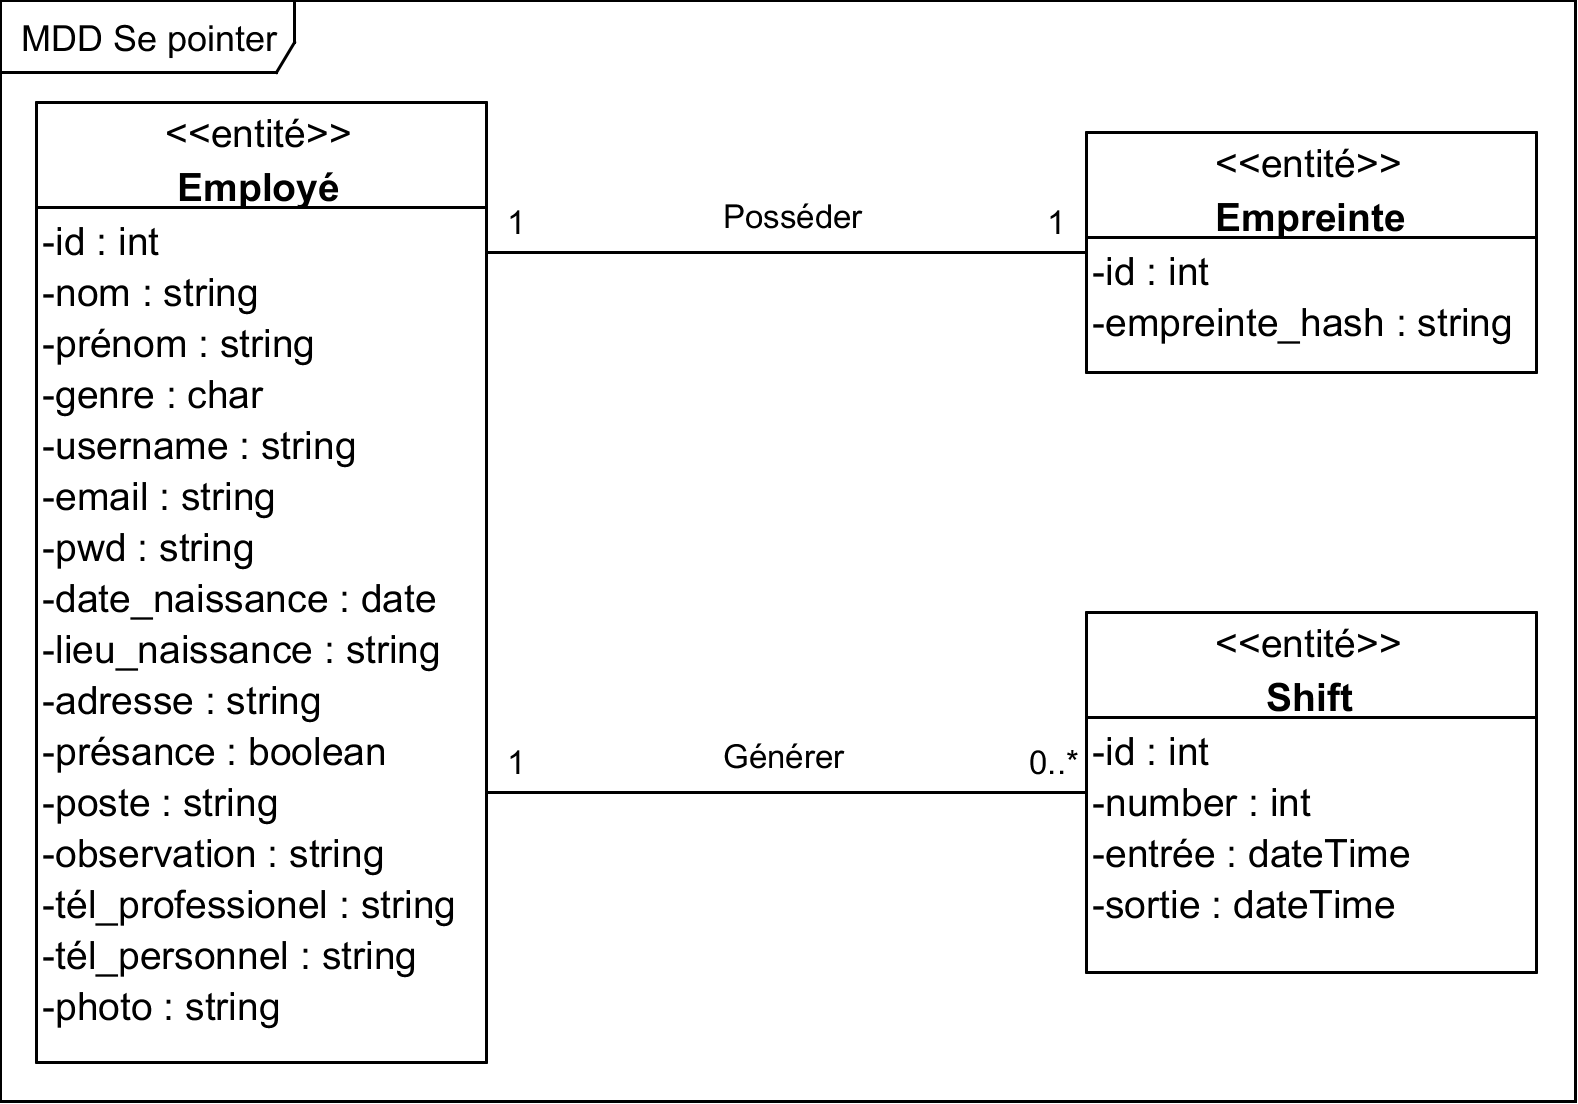
\includegraphics[scale=1.3]{images/MDD/MDD Se pointer.png}
    \caption{Modèle du domaine « Se pointer »}
    \label{fig12}
\end{figure}


\subsection*{Modèle du domaine du cas d'utilisation « Consulter ma fiche de pointage »}
Ce diagramme du modèle du domaine représente les entités concernées par le cas 
« Consulter ma fiche de pointage ». On peut distinguer deux entités: employé 
et Shift (qui représente une période de temps délimité par un temps d’entrée et 
un temps de sortie et la date de ces deux évènements).

\clearpage

\begin{figure}[h!]
    \centering
    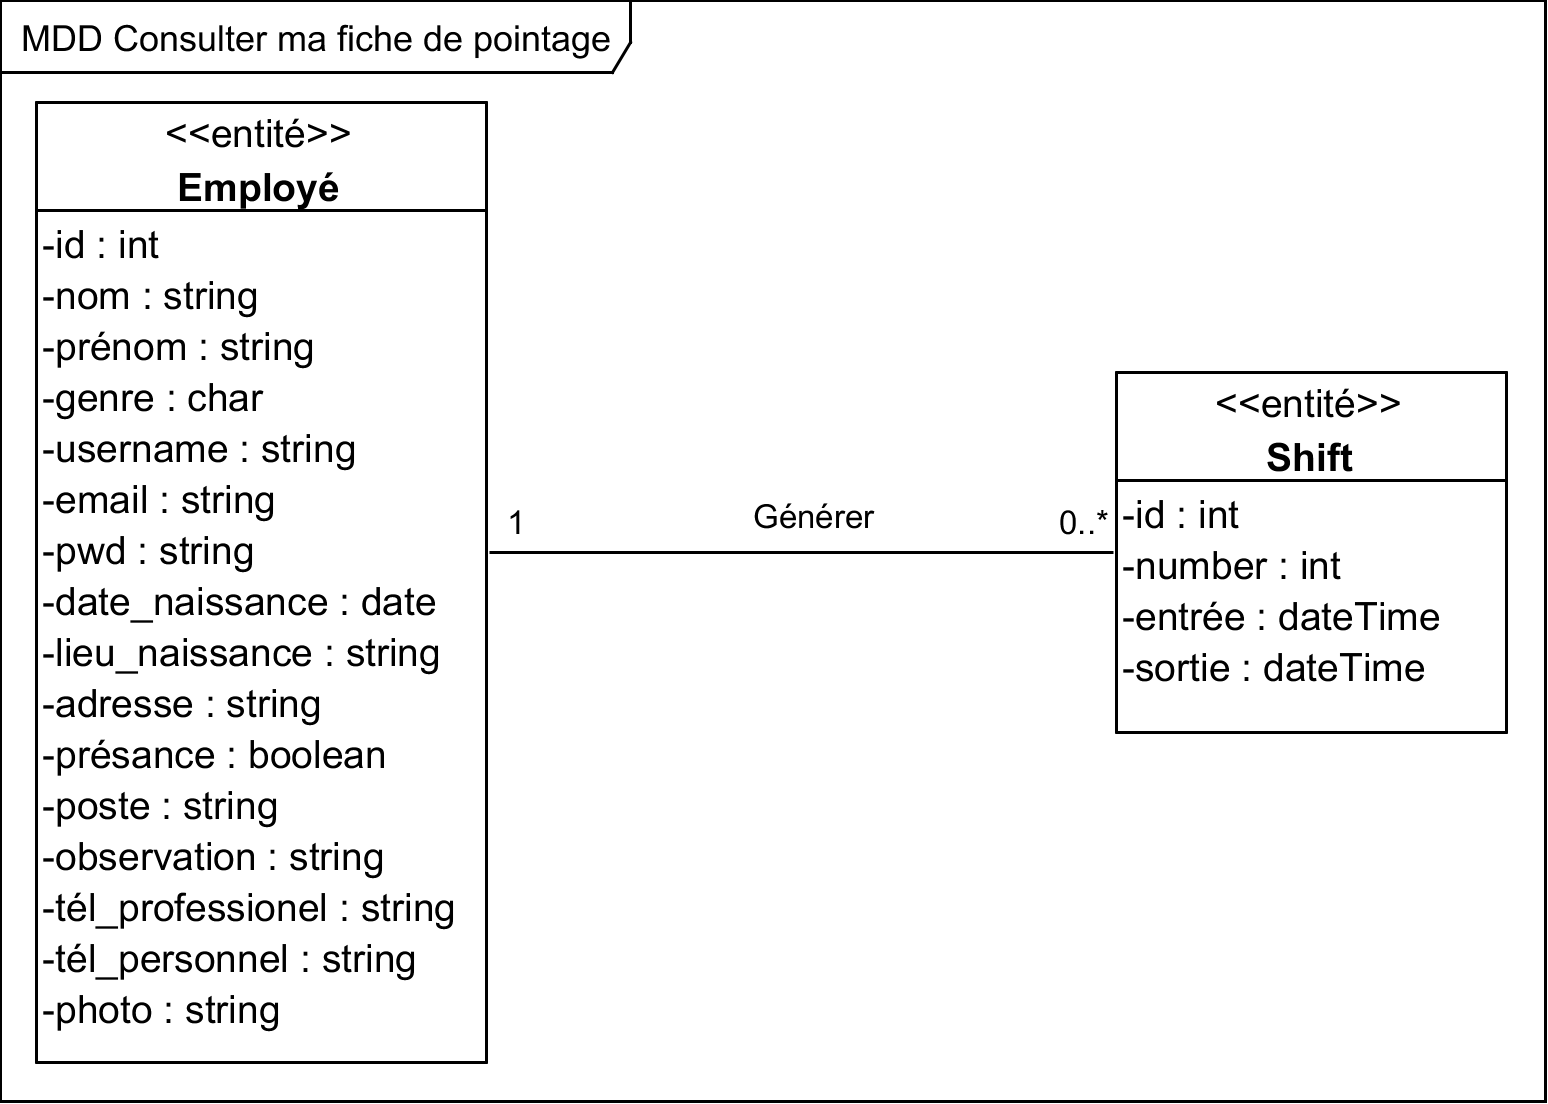
\includegraphics[scale=1.168]{images/MDD/MDD Consulter ma fiche de pointage.png}
    \caption{Modèle du domaine « Consulter ma fiche de pointage »}
    \label{fig13}
\end{figure}
            
\subsection*{Modèle du domaine du cas d'utilisation « Ajouter planning »}
Ce modèle du domaine exprime le fait qu’un planning est composé de sept jours. 
Dans lesquels nous retrouvons deux parties qui représente une journée de travail 
d’un employé.

\begin{figure}[h!]
    \centering
    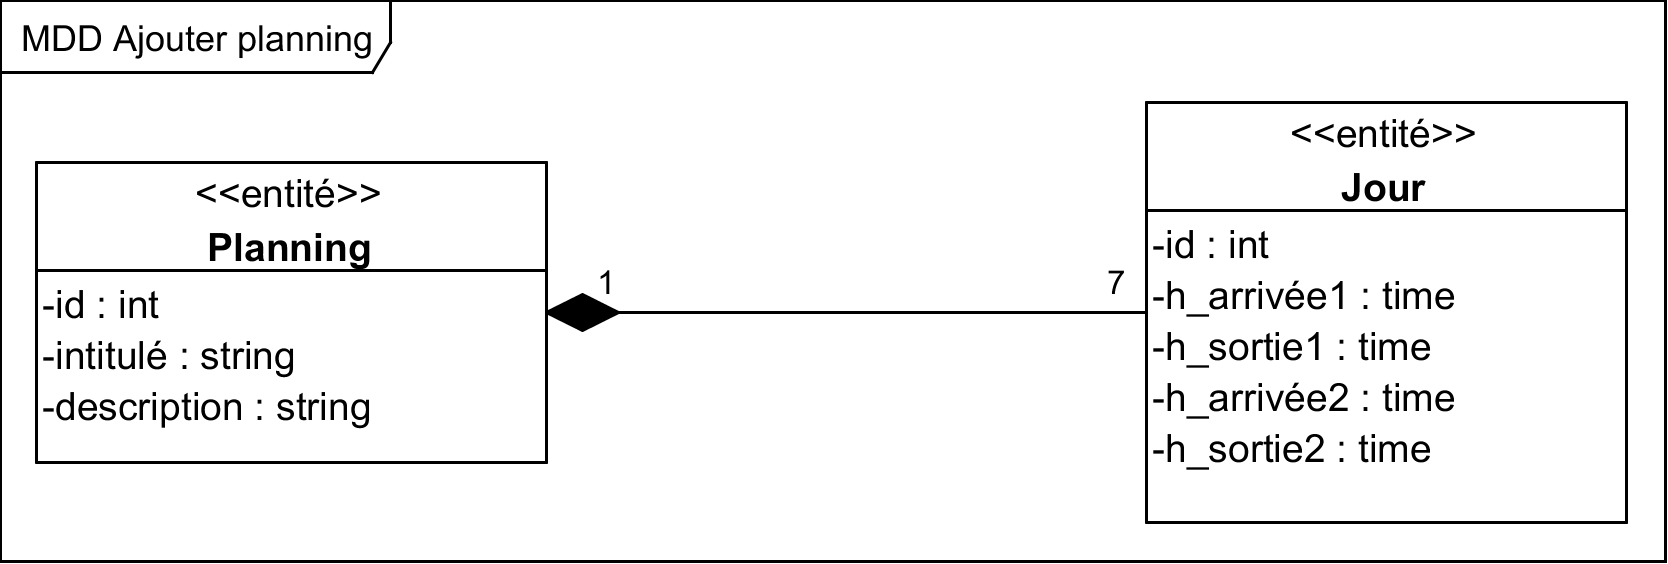
\includegraphics[scale=1.12]{images/MDD/MDD Ajouter planning.png}
    \caption{Modèle du domaine « Ajouter planning »}
    \label{fig14}
\end{figure}
        
\subsection*{Modèle du domaine du cas d'utilisation « Ajouter équipe »}
Sur ce modèle du domaine on remarque que les entités sont reliées par 
deux associations. Une représente le fait d’être membre d’une équipe, et 
l’autre le fait de gérer (ou manager) une équipe. Nous avons décidé de relier
cette association à l’employé et non au manager (qui hérite de l’employé), car
nous estimons qu’à ce stade il n’y a pas d'attributs liés exclusivement au
manager (il se pourrait que cela se fera dans les prochains diagrammes en raison
des méthodes).  

\begin{figure}[h!]
    \centering
    \includegraphics[scale=1.38]{images/MDD/MDD Ajouter équipe.png}
    \caption{Modèle du domaine « Ajouter équipe »}
    \label{fig15}
\end{figure}
            
\subsection*{Modèle du domaine du cas d'utilisation « Ajouter employé »}
Sur ce modèle du domaine figurent deux entités capitales de notre système 
qui sont l’employé et son empreinte. Il est important de noter qu’un employé 
ne peut avoir qu’une seule empreinte dans le système (index droit).

\clearpage

\begin{figure}[h!]
    \centering
    \includegraphics[scale=1.4]{images/MDD/MDD Ajouter employé.png}
    \caption{Modèle du domaine « Ajouter employé »}
    \label{fig16}
\end{figure}
            
\subsection*{Modèle du domaine du cas d'utilisation « Ajouter membre »}
En plus des deux entités, précédemment citées dans le modèle du domaine du cas 
d’utilisation « Ajouter équipe », on retrouve une classe d’association qui 
nous permet de garder une trace du changement d’équipe pour chaque employé.

\clearpage

\begin{figure}[h!]
	\centering
	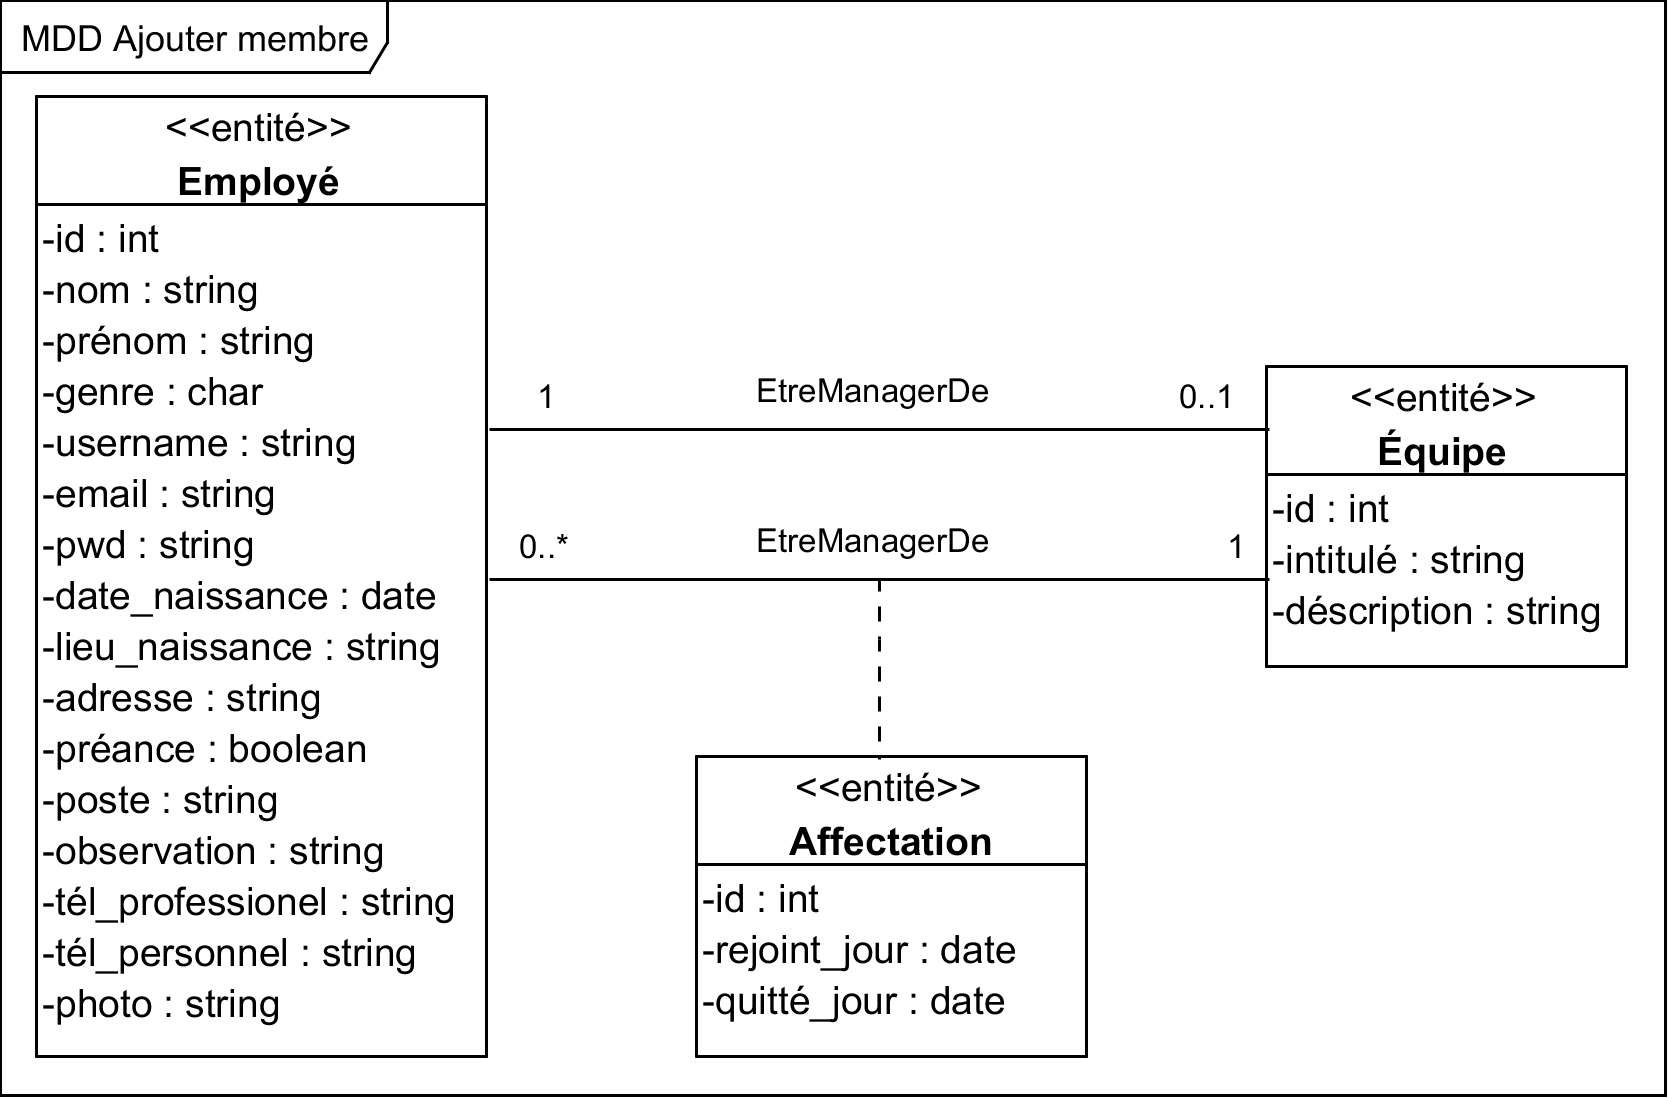
\includegraphics[scale=1.22]{images/MDD/MDD Ajouter membre.png}
	\caption{Diagramme de séquence système « Ajouter membre »}
	\label{fig17}
\end{figure}


\subsection*{Modèle du domaine du cas d'utilisation « Consulter profil d'un employé »}
Sur ce modèle du domaine, le but est d’offrir aux employés un planning 
flexible. Pour ce faire, nous avons une composition entre 2 entités: un
\emph{planning} qui est la classe mère avec comme attributs un intitulé du
planning ainsi qu’une description, et une classe \emph{jour} qui modélise les
jours de la semaine avec comme attributs les horaires de travails.

\clearpage

\begin{figure}[h!]
    \centering
    \includegraphics[scale=1.32]{images/MDD/MDD Consulter profil d'un employé.png}
    \caption{Modèle du domaine « Consulter profil d'un employé »}
    \label{fig18}
\end{figure}
            
\subsection*{Modèle du domaine du cas d'utilisation « Consulter tableau de bord manager »}
Sur ce modèle du domaine, on peut observer que plusieurs entités participent à
la réalisation du cas d’utilisation. Ceci est dû à sa nature sommaire. Un
tableau de bord se doit d’être récapitulatif et offrir un maximum d’informations
pertinentes en un minimum d’espace. Pour avoir la liste des collaborateurs, nous
avons besoins des deux entités: \emph{employé} et \emph{équipe}. Afin de savoir
si un collaborateur est en retard ou absent, on doit accéder à son planning. 

\begin{figure}[h!]
    \centering
    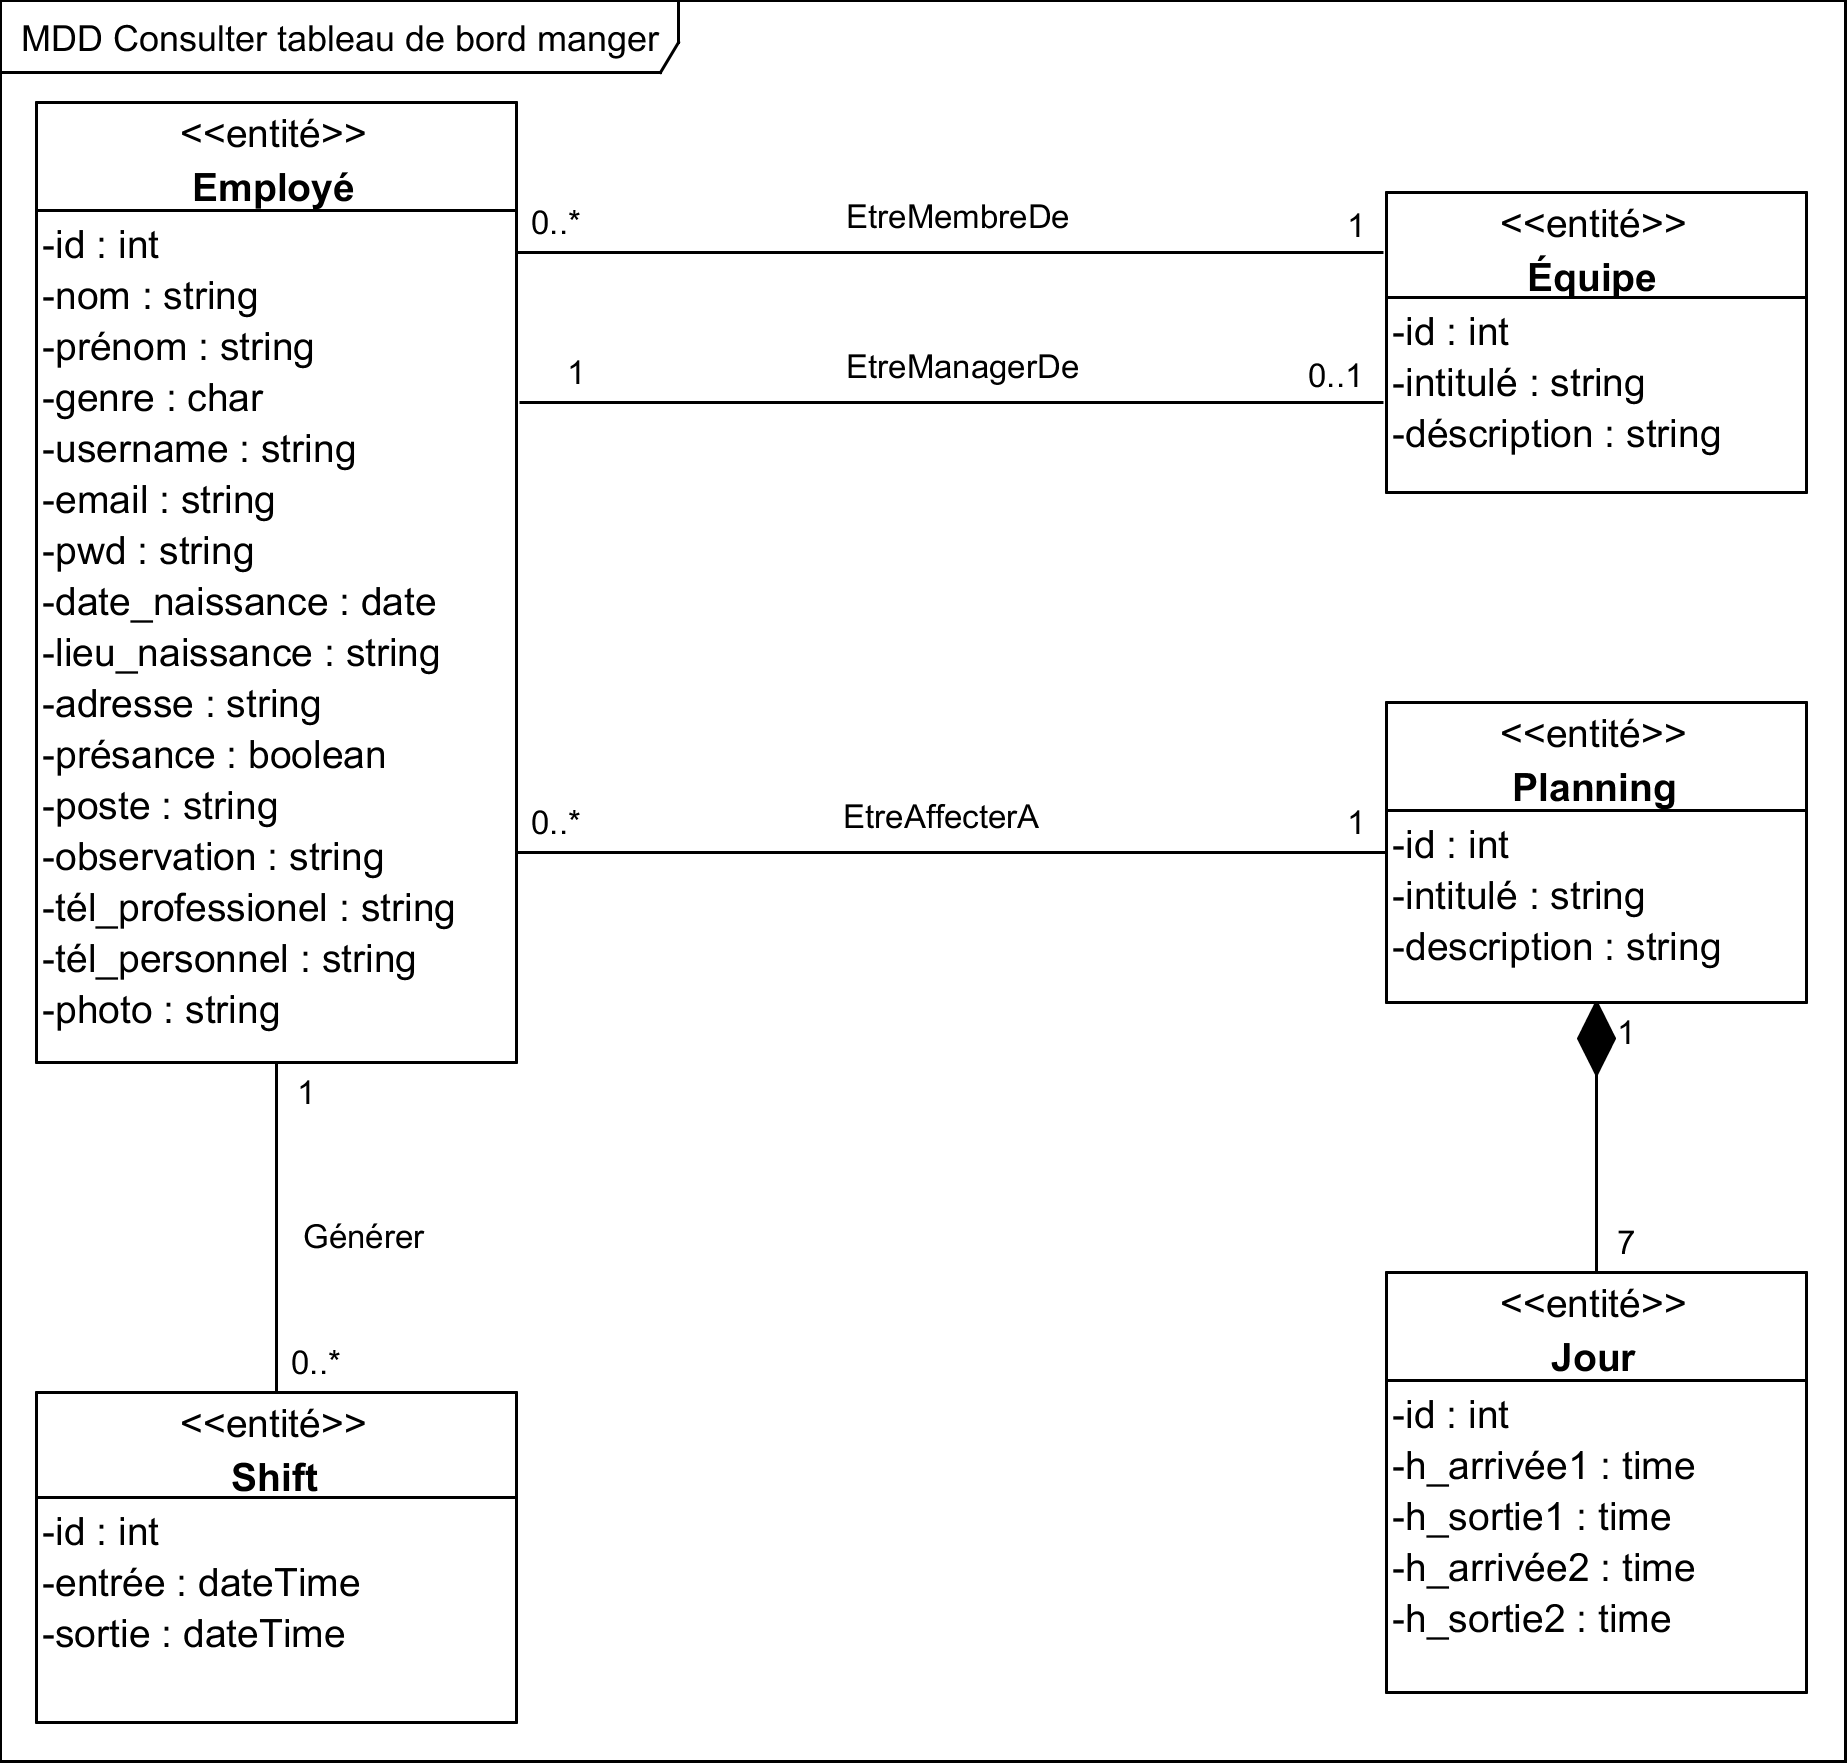
\includegraphics[scale=1.06]{images/MDD/MDD Consulter tableu de bord manger.png}
    \caption{Modèle du domaine « Consulter tableau de bord manager »}
    \label{fig19}
\end{figure}
            
\section{Diagrammes de classes participantes}
L’importance du diagramme de classes participantes réside dans le fait qu’il
effectue la jonction entre les cas d’utilisation, les classes d’analyse et
l’interface avec l’utilisateur, de plus, il permet l’enrichissement des
diagrammes de séquence système.\cite{8}

\subsection{Définitions et formalisme}
Les classes composant un diagramme de classes participantes se répartissent en
trois catégories:\cite{6}

\subsubsection{Les classes de dialogue}
Ces classes permettent les interactions entre l’IHM et les utilisateurs. 
Il s’agit typiquement des écrans proposés à l’utilisateur: les formulaires de 
saisie, les résultats de recherche, etc. En général, les dialogues vivent 
seulement le temps du déroulement du cas d’utilisation concerné, afin de 
modéliser une classe de dialogue nous allons utiliser le modèle de la 
figure\ref{fig20}.

\begin{figure}[h!]
    \centering
    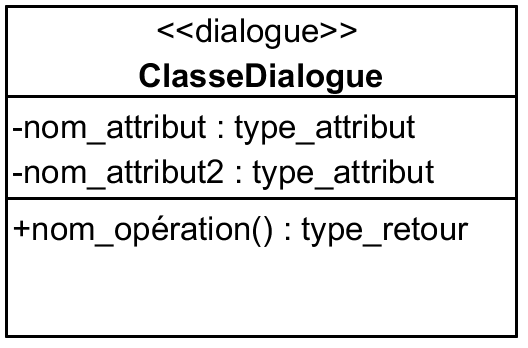
\includegraphics[scale=1.5]{images/dialogue.png}
    \caption{Représentation d'une classe dialogue}
    \label{fig20}
\end{figure}
        
\subsubsection{Les classes de contrôle}
Les classes qui modélisent la cinématique de l’application sont appelées 
contrôles. Elles font la jonction entre les dialogues et les classes métier en 
permettant aux différentes vues de l’application de manipuler des informations 
détenues par des objets métier. Elles contiennent les règles applicatives et les 
isolent à la fois des dialogues et des entités, elles seront représentées comme 
sur la figure\ref{fig21}.

\begin{figure}[h!]
    \centering
    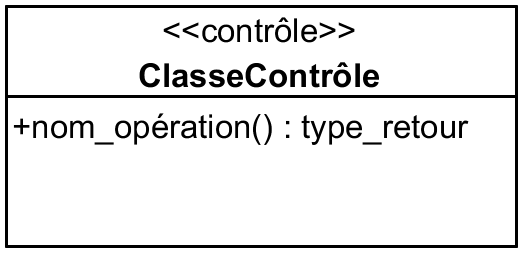
\includegraphics[scale=1.5]{images/Controle.png}
    \caption{Représentation d'une classe contrôle}
    \label{fig21}
\end{figure}
        
\subsubsection{Les classes entités}
Les classes métier, qui proviennent directement du modèle du domaine sont 
qualifiées d’entités. Ces classes sont généralement persistantes, 
c’est à dire qu’elles survivent à l’exécution d’un cas d’utilisation 
particulier et qu’elles permettent à des données et à des relations d’être 
stockées dans des fichiers ou des bases de données. Elles seront 
représentées comme sur la figure\ref{fig22}.

\clearpage

\begin{figure}[h!]
    \centering
    \includegraphics[scale=1.5]{images/Entité.png}
    \caption{Représentation d'une classe entité}
    \label{fig22}
\end{figure}
        
Afin d’établir un DCP, nous ajouterons des associations entre les classes tout 
en respectant les règles ci-après: \cite{5}

\begin{itemize}
    \item[\textbullet] Les dialogues ne peuvent être reliés qu'aux contrôles ou à 
        d'autres dialogues, mais pas directement aux entités.
    \item [\textbullet] Les entités ne peuvent être reliées qu'aux contrôles ou à 
        d'autres entités.
    \item [\textbullet] Les contrôles ont accès à tous les types de classes, y 
        compris d'autres contrôles.
    \item [\textbullet] Enfin, un acteur ne peut être lié qu'à un dialogue.
\end{itemize}

Un exemple de diagramme de classe participante est représenté dans la figure 
ci-dessous:  

\begin{figure}[h!]
    \centering
    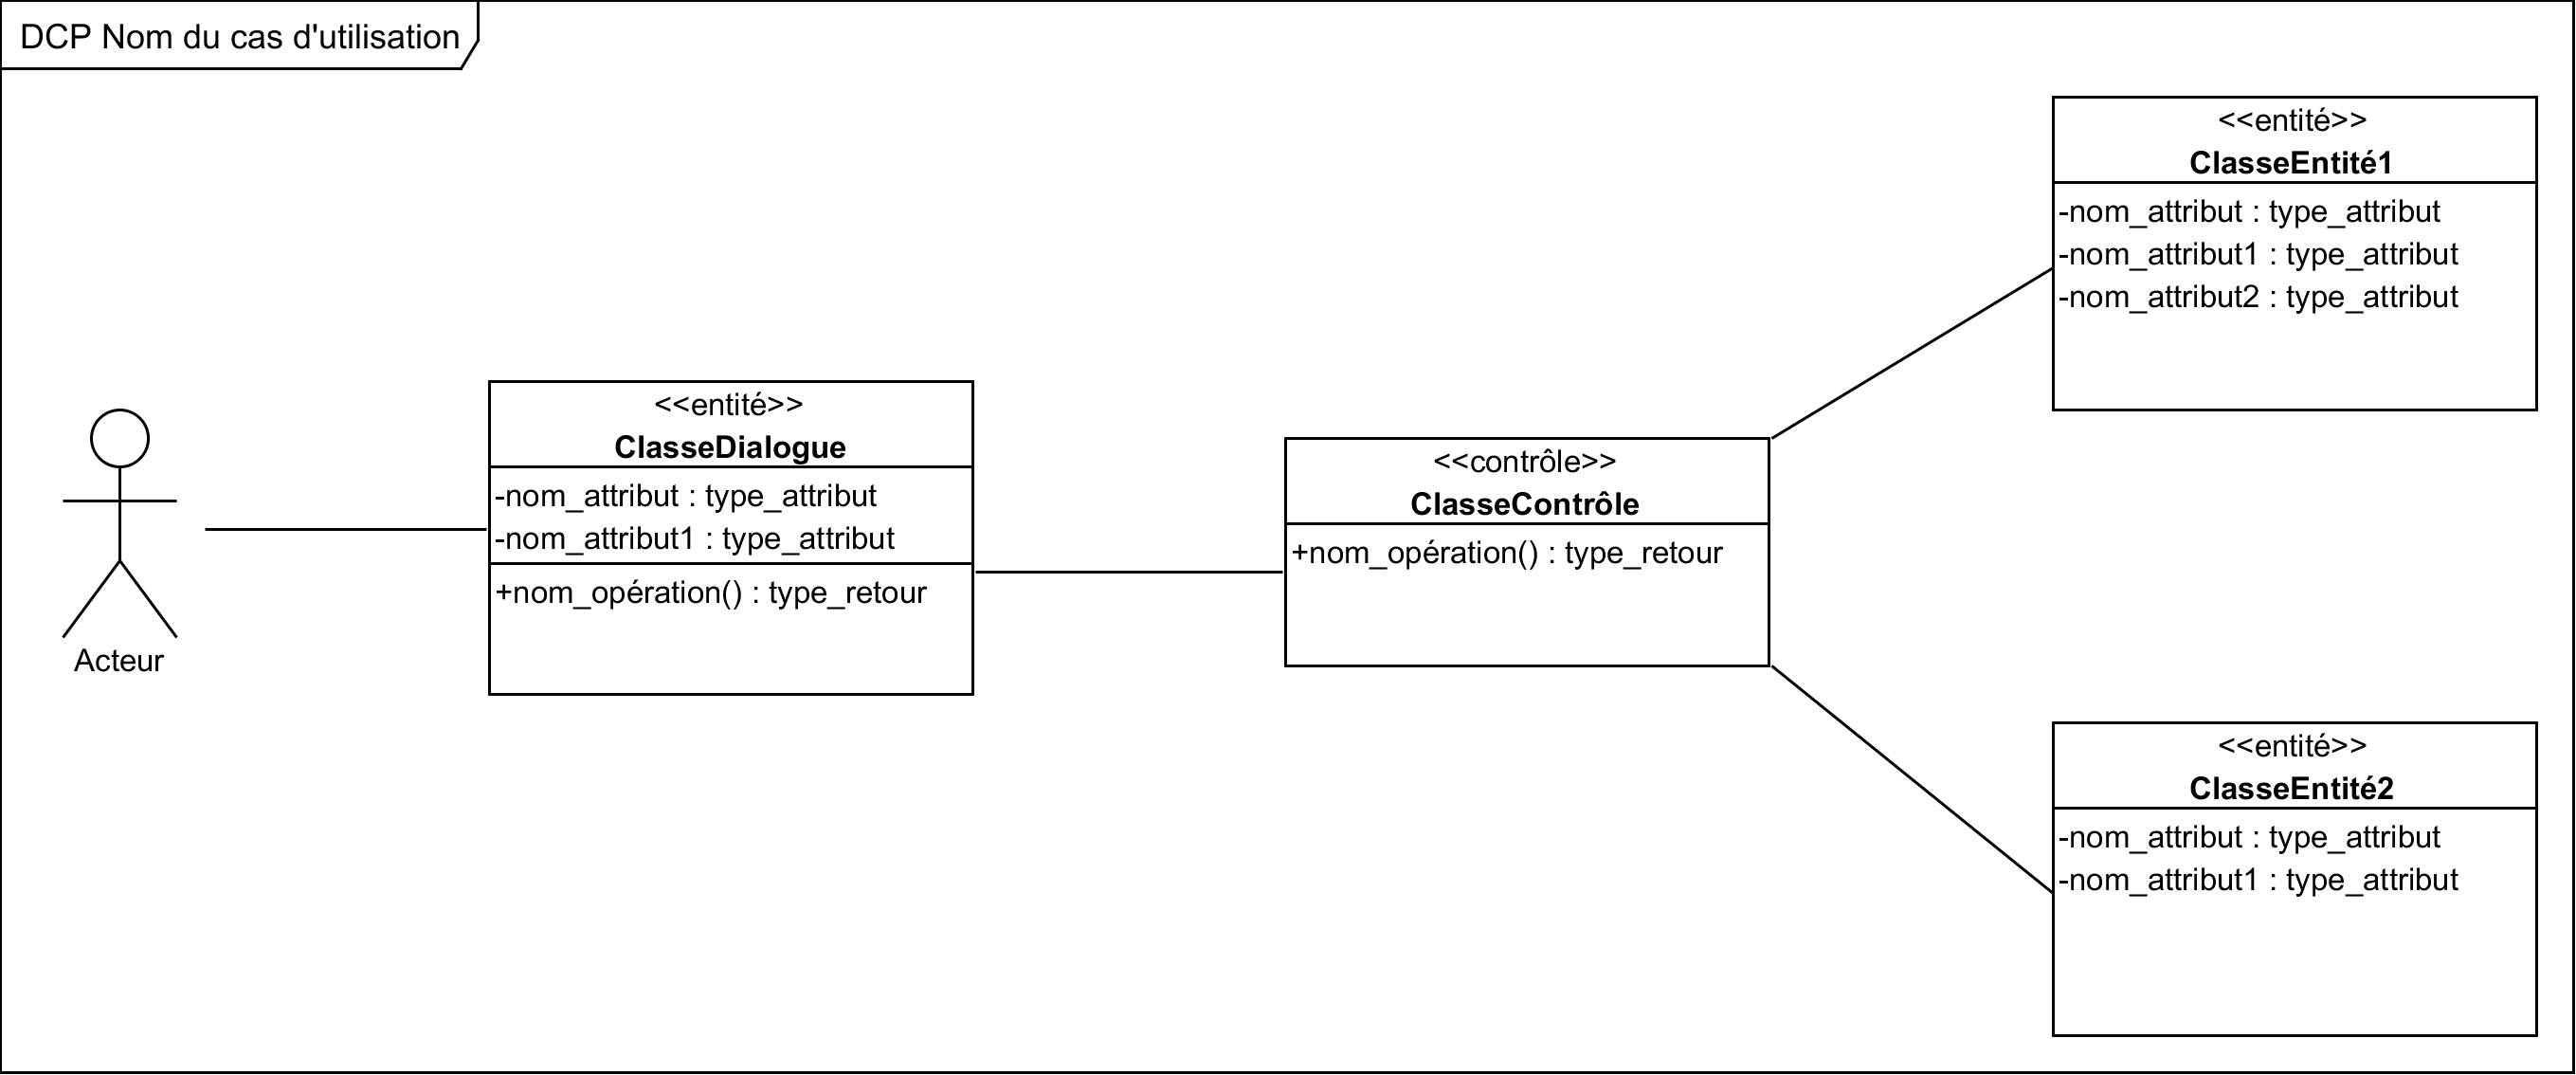
\includegraphics[scale=0.74]{images/DCP_exemple.png}
    \caption{Modèle d'un diagramme de classe de conception}
    \label{fig23}
\end{figure}

\clearpage

\subsection*{Diagrammes de classes participantes du cas d'utilisation « Se pointer »}
La pointeuse biométrique permet à l’employé d’enregistrer ses horaires de 
travails le plus facilement possible. Pour ce qui est de la logique concernant 
les actions effectuées par l’employé, elle est déléguée à trois contrôleurs: 
CtrShift et CtrEmployé et CtrEmpreinte.
            
\begin{figure}[h!]
    \centering
    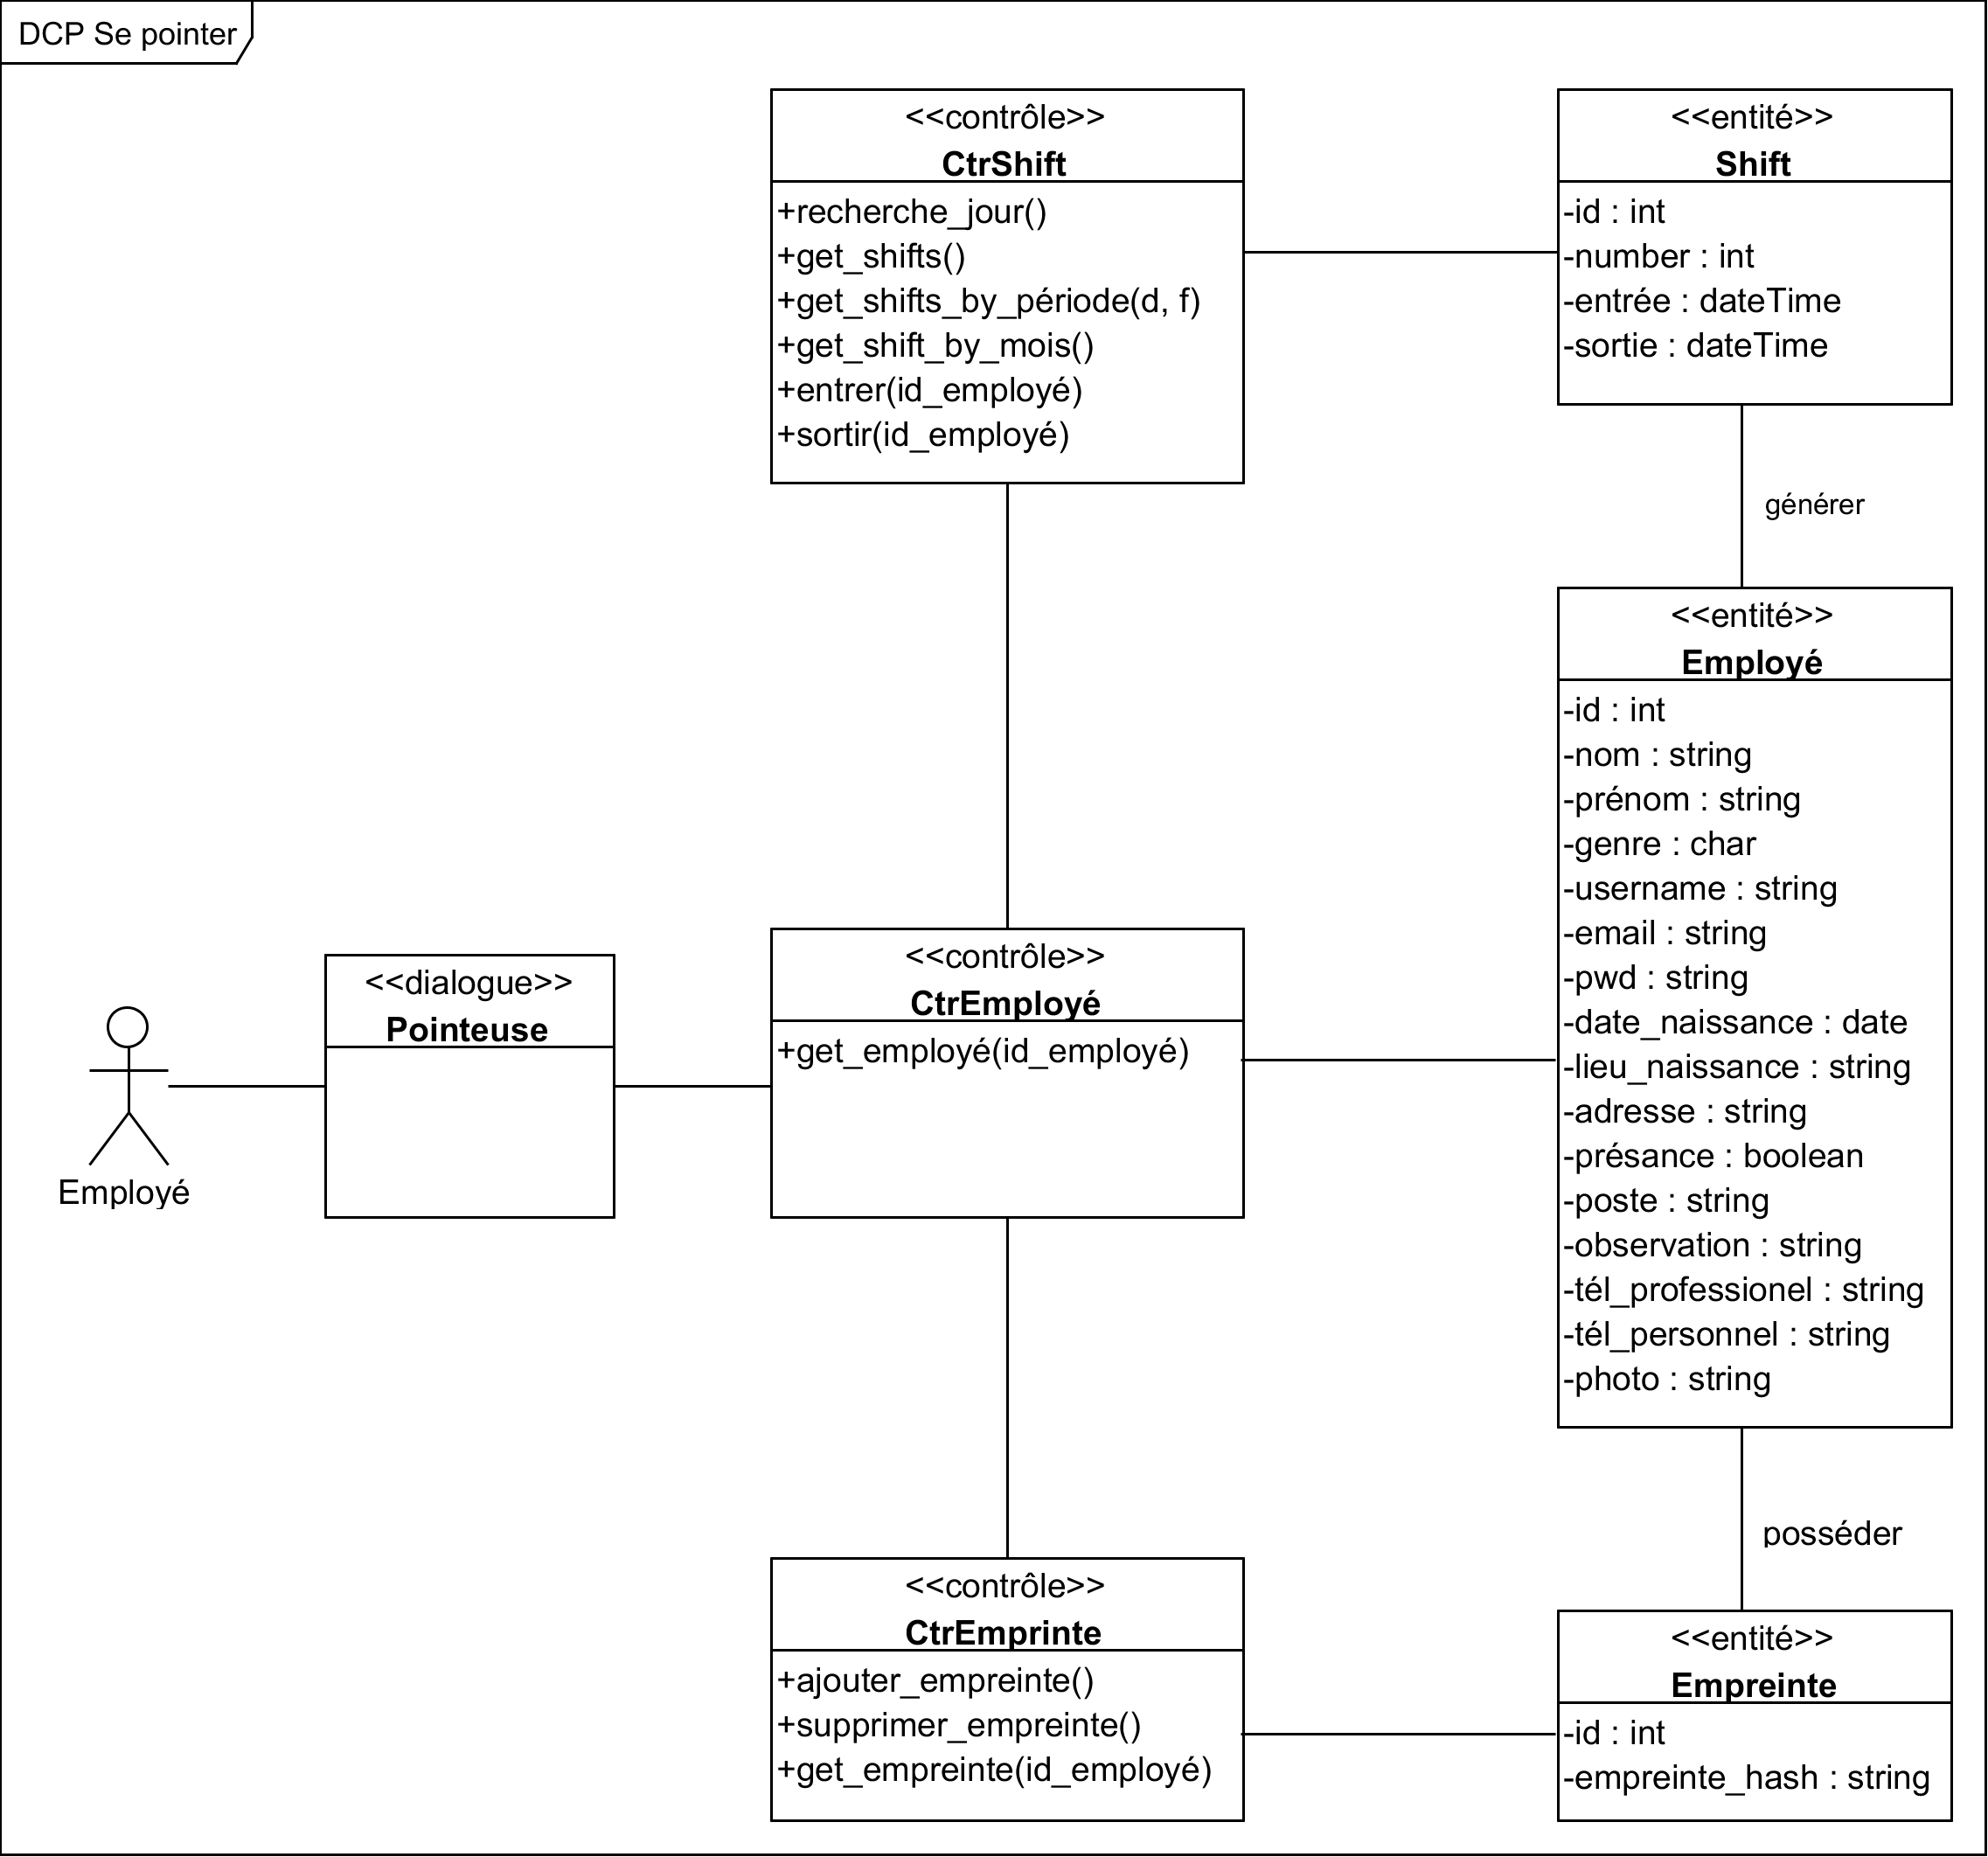
\includegraphics[scale=0.84]{images/DCP/DCP Se pointer.png}
    \caption{Diagrammes de classes participantes « Consulter ma fiche de pointage »}
    \label{fig24}
\end{figure}
            
\subsection*{Diagrammes de classes participantes du cas d'utilisation « Consulter mon profil »}
Un employé peut consulter son profil sur l’interface « InterfaceMonProfil » qui 
regroupe ses informations, il peut aussi accéder à l’interface de modification 
de son profil, ainsi qu’afficher son planning. Les actions effectuées sont 
gérées par le contrôleur CtrEmployé.  

\begin{figure}[h!]
    \centering
    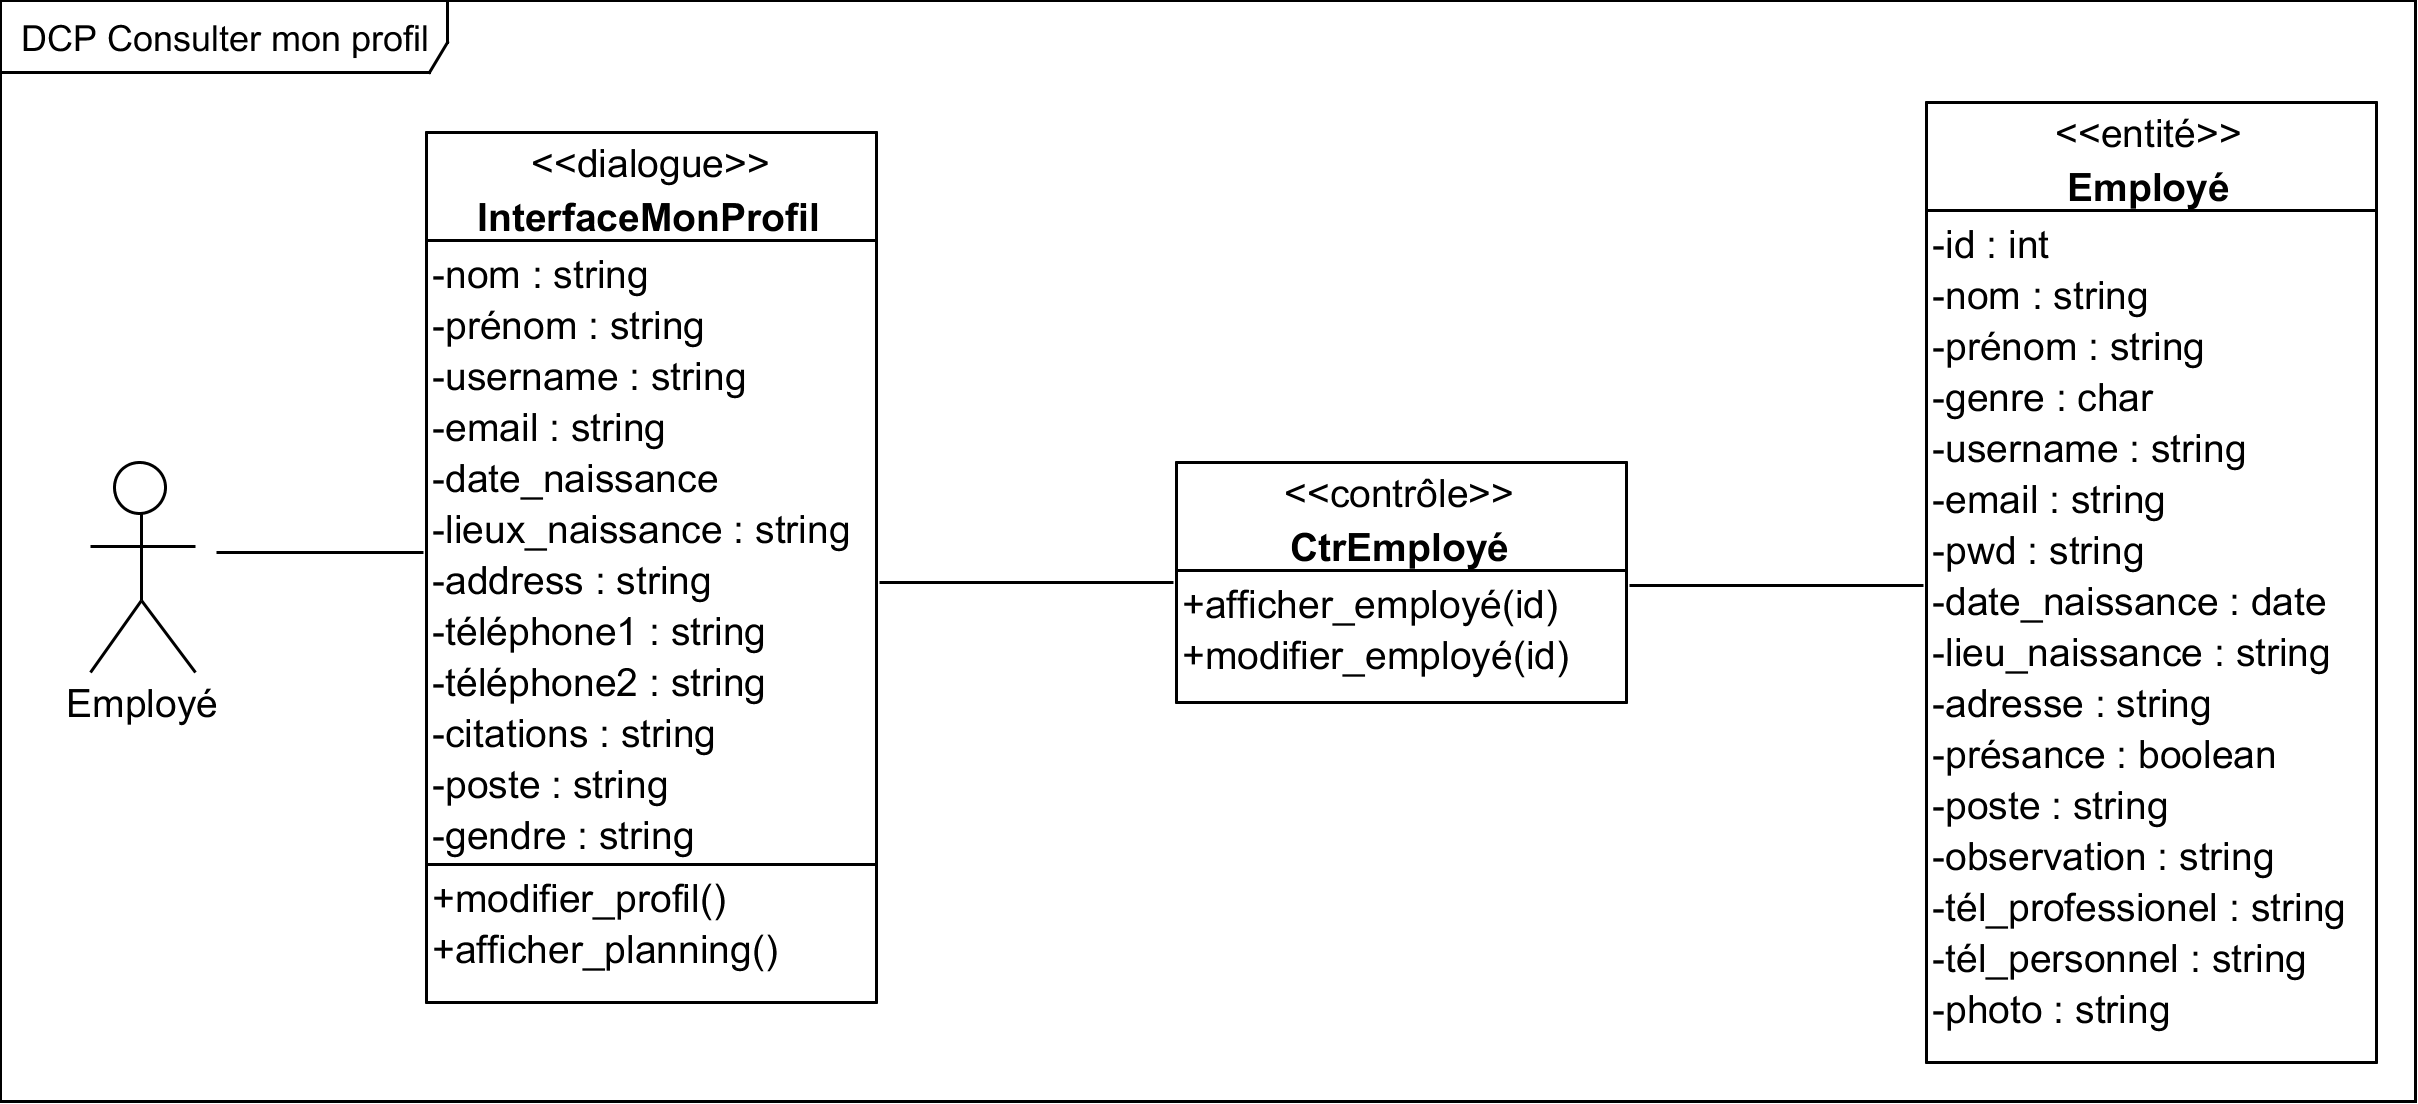
\includegraphics[scale=0.7]{images/DCP/DCP consulter_mon_profil.png}
    \caption{Diagrammes de classes participantes « Consulter mon profil »}
    \label{fig25}
\end{figure}
        
\subsection*{Diagrammes de classes participantes du cas d'utilisation « Consulter ma fiche de pointage »}
Un employé peut consulter sa fiche de pointage sur l’interface «
InterfaceConsulterMaFichePointage ». Par défaut, l’affichage de la liste des
pointages est par semaine, s’il le souhaite il peut l’afficher par mois ou faire
une recherche précise par période. La logique concernant les actions effectuées
par l’employé est déléguée à deux contrôleurs: CtrShift et CtrEmployé.
            
\begin{figure}[h!]
    \centering
    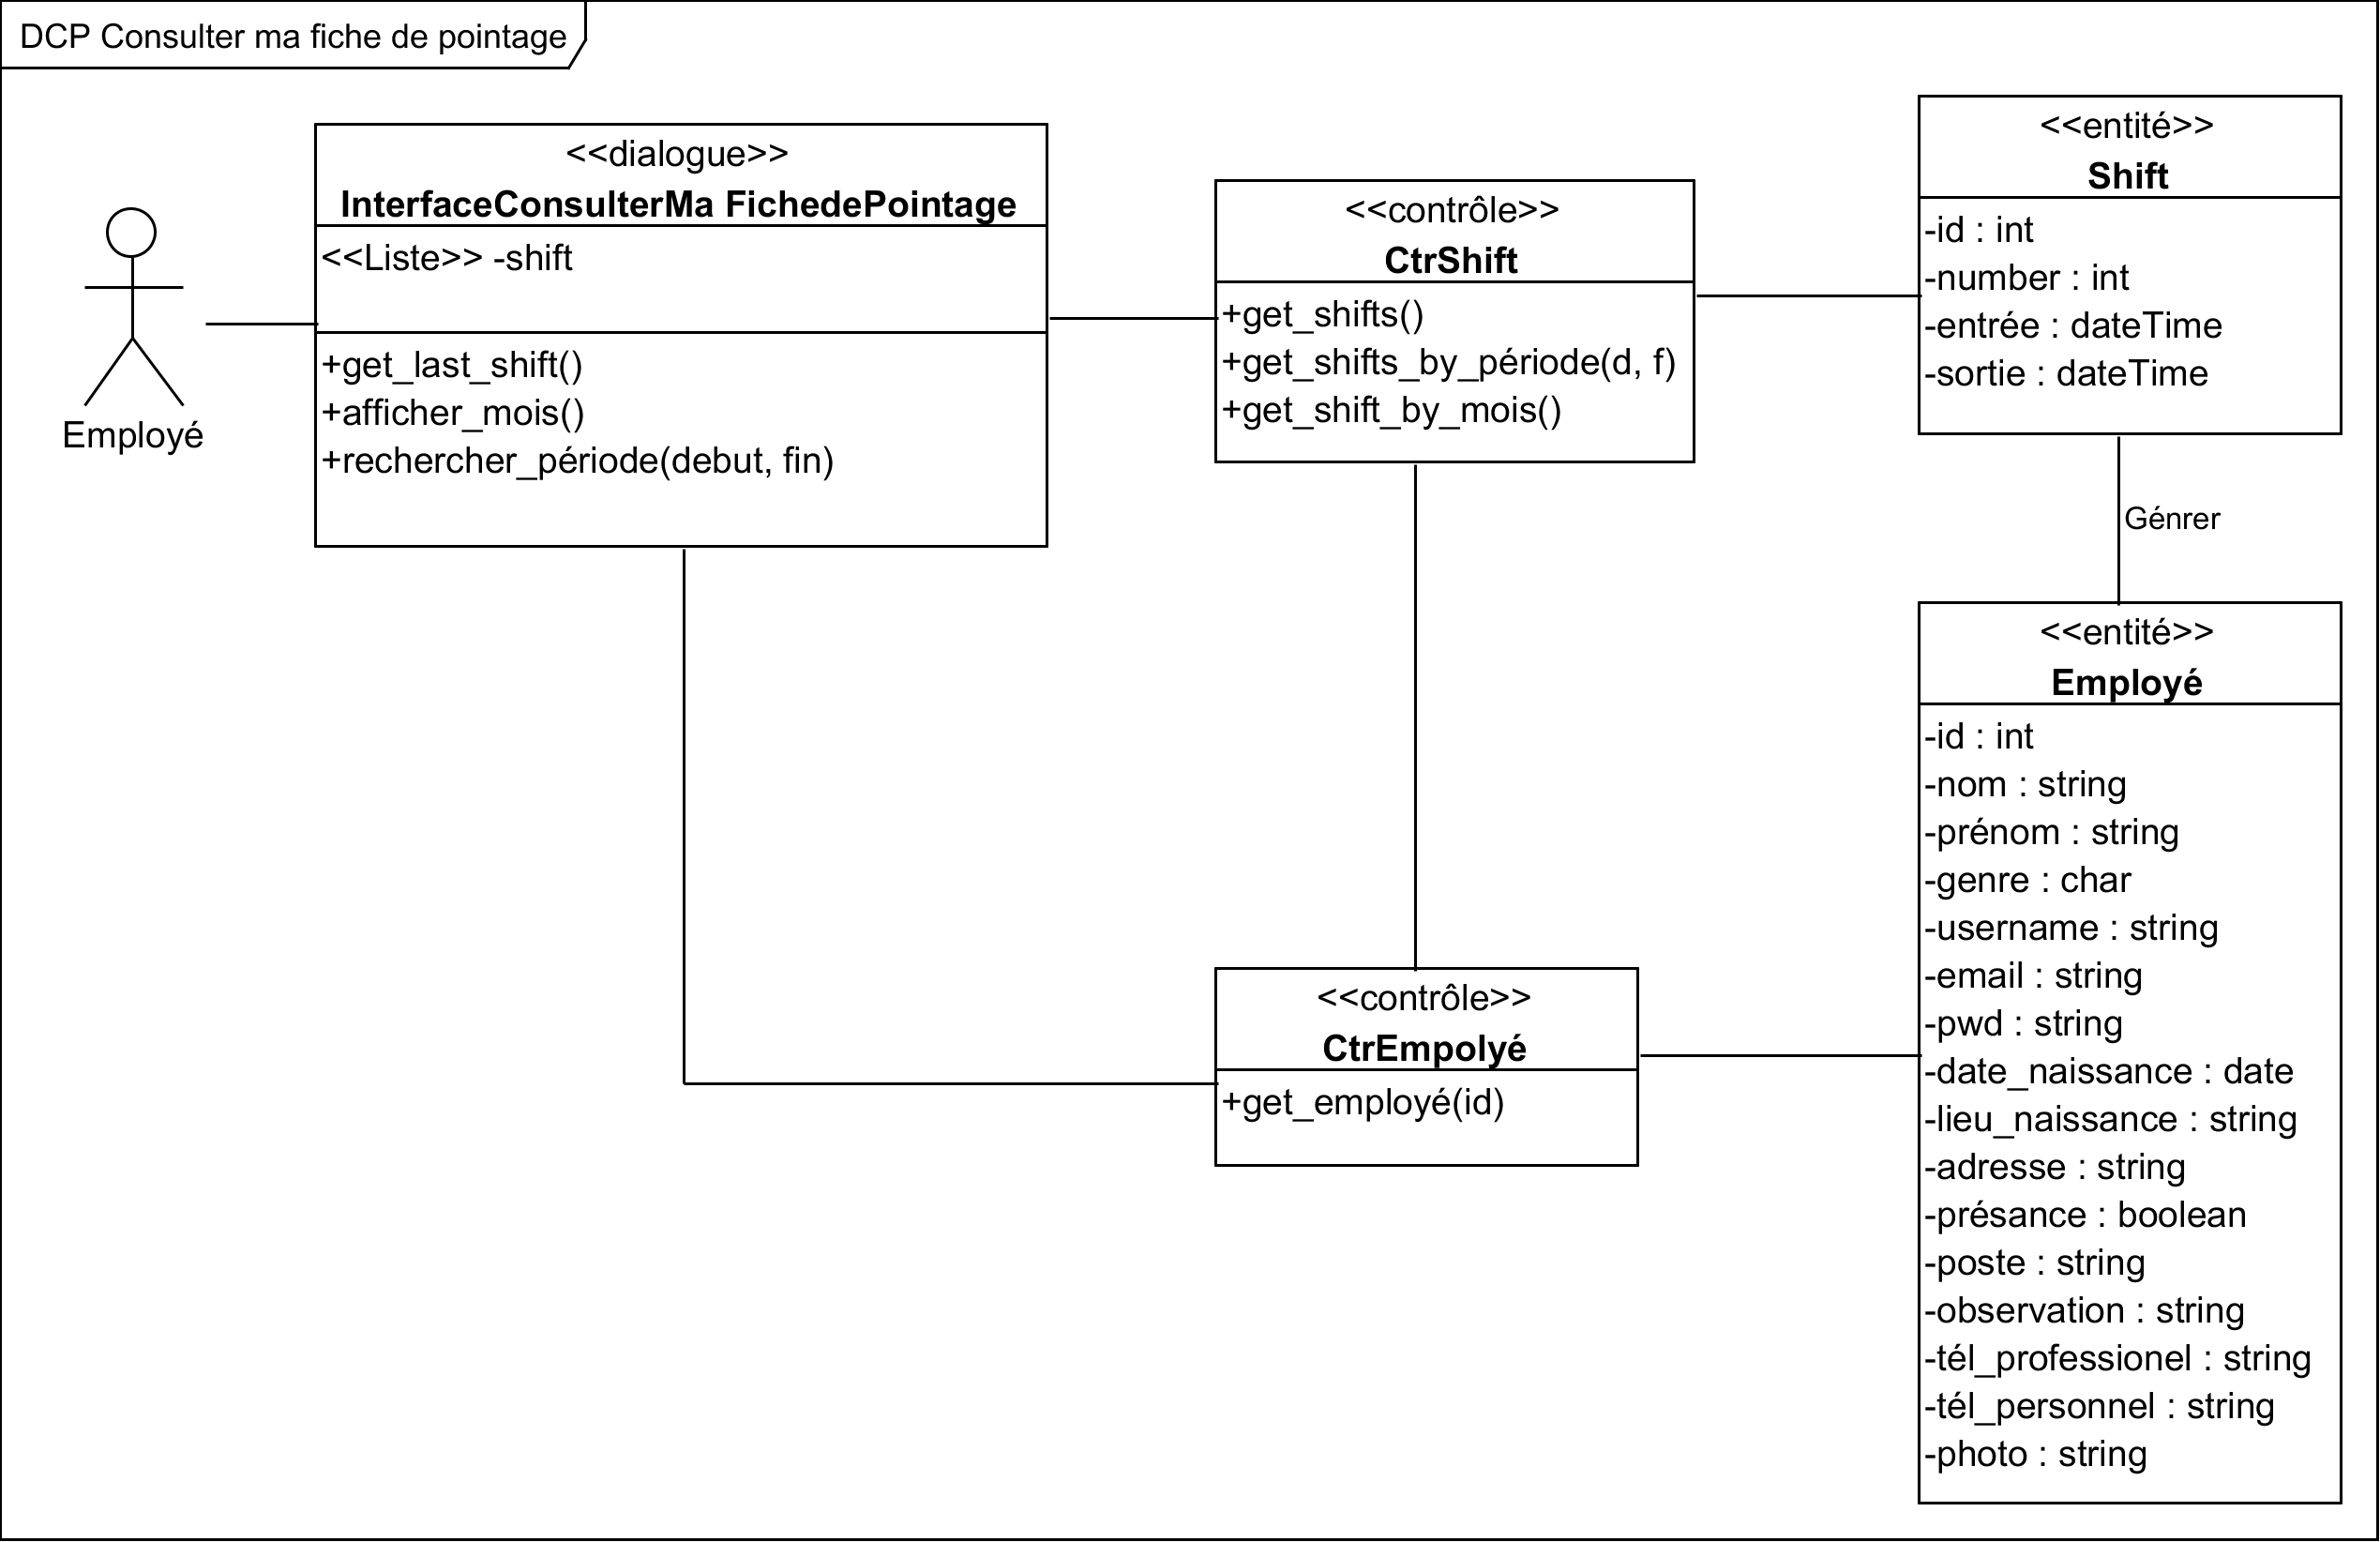
\includegraphics[scale=0.72]{images/DCP/DCP Consulter ma fiche de pointage.png}
    \caption{Diagrammes de classes participantes « Consulter ma fiche de pointage »}
    \label{fig26}
\end{figure}
            
\subsection*{Diagrammes de classes participantes du cas d'utilisation « Consulter tableau de bord manager »}
Une fois authentifié, le manager est redirigé vers 
« InterfaceTableauBordManager » où il aura accès à son planning du jour, une 
liste de ces collaborateurs, ainsi qu’un résumé sur l’ensemble de ces équipes. 
Les 2 contrôles CtrEmployés et CtrEquipe traitent les actions du manager. 

\begin{figure}[h!]
    \centering
    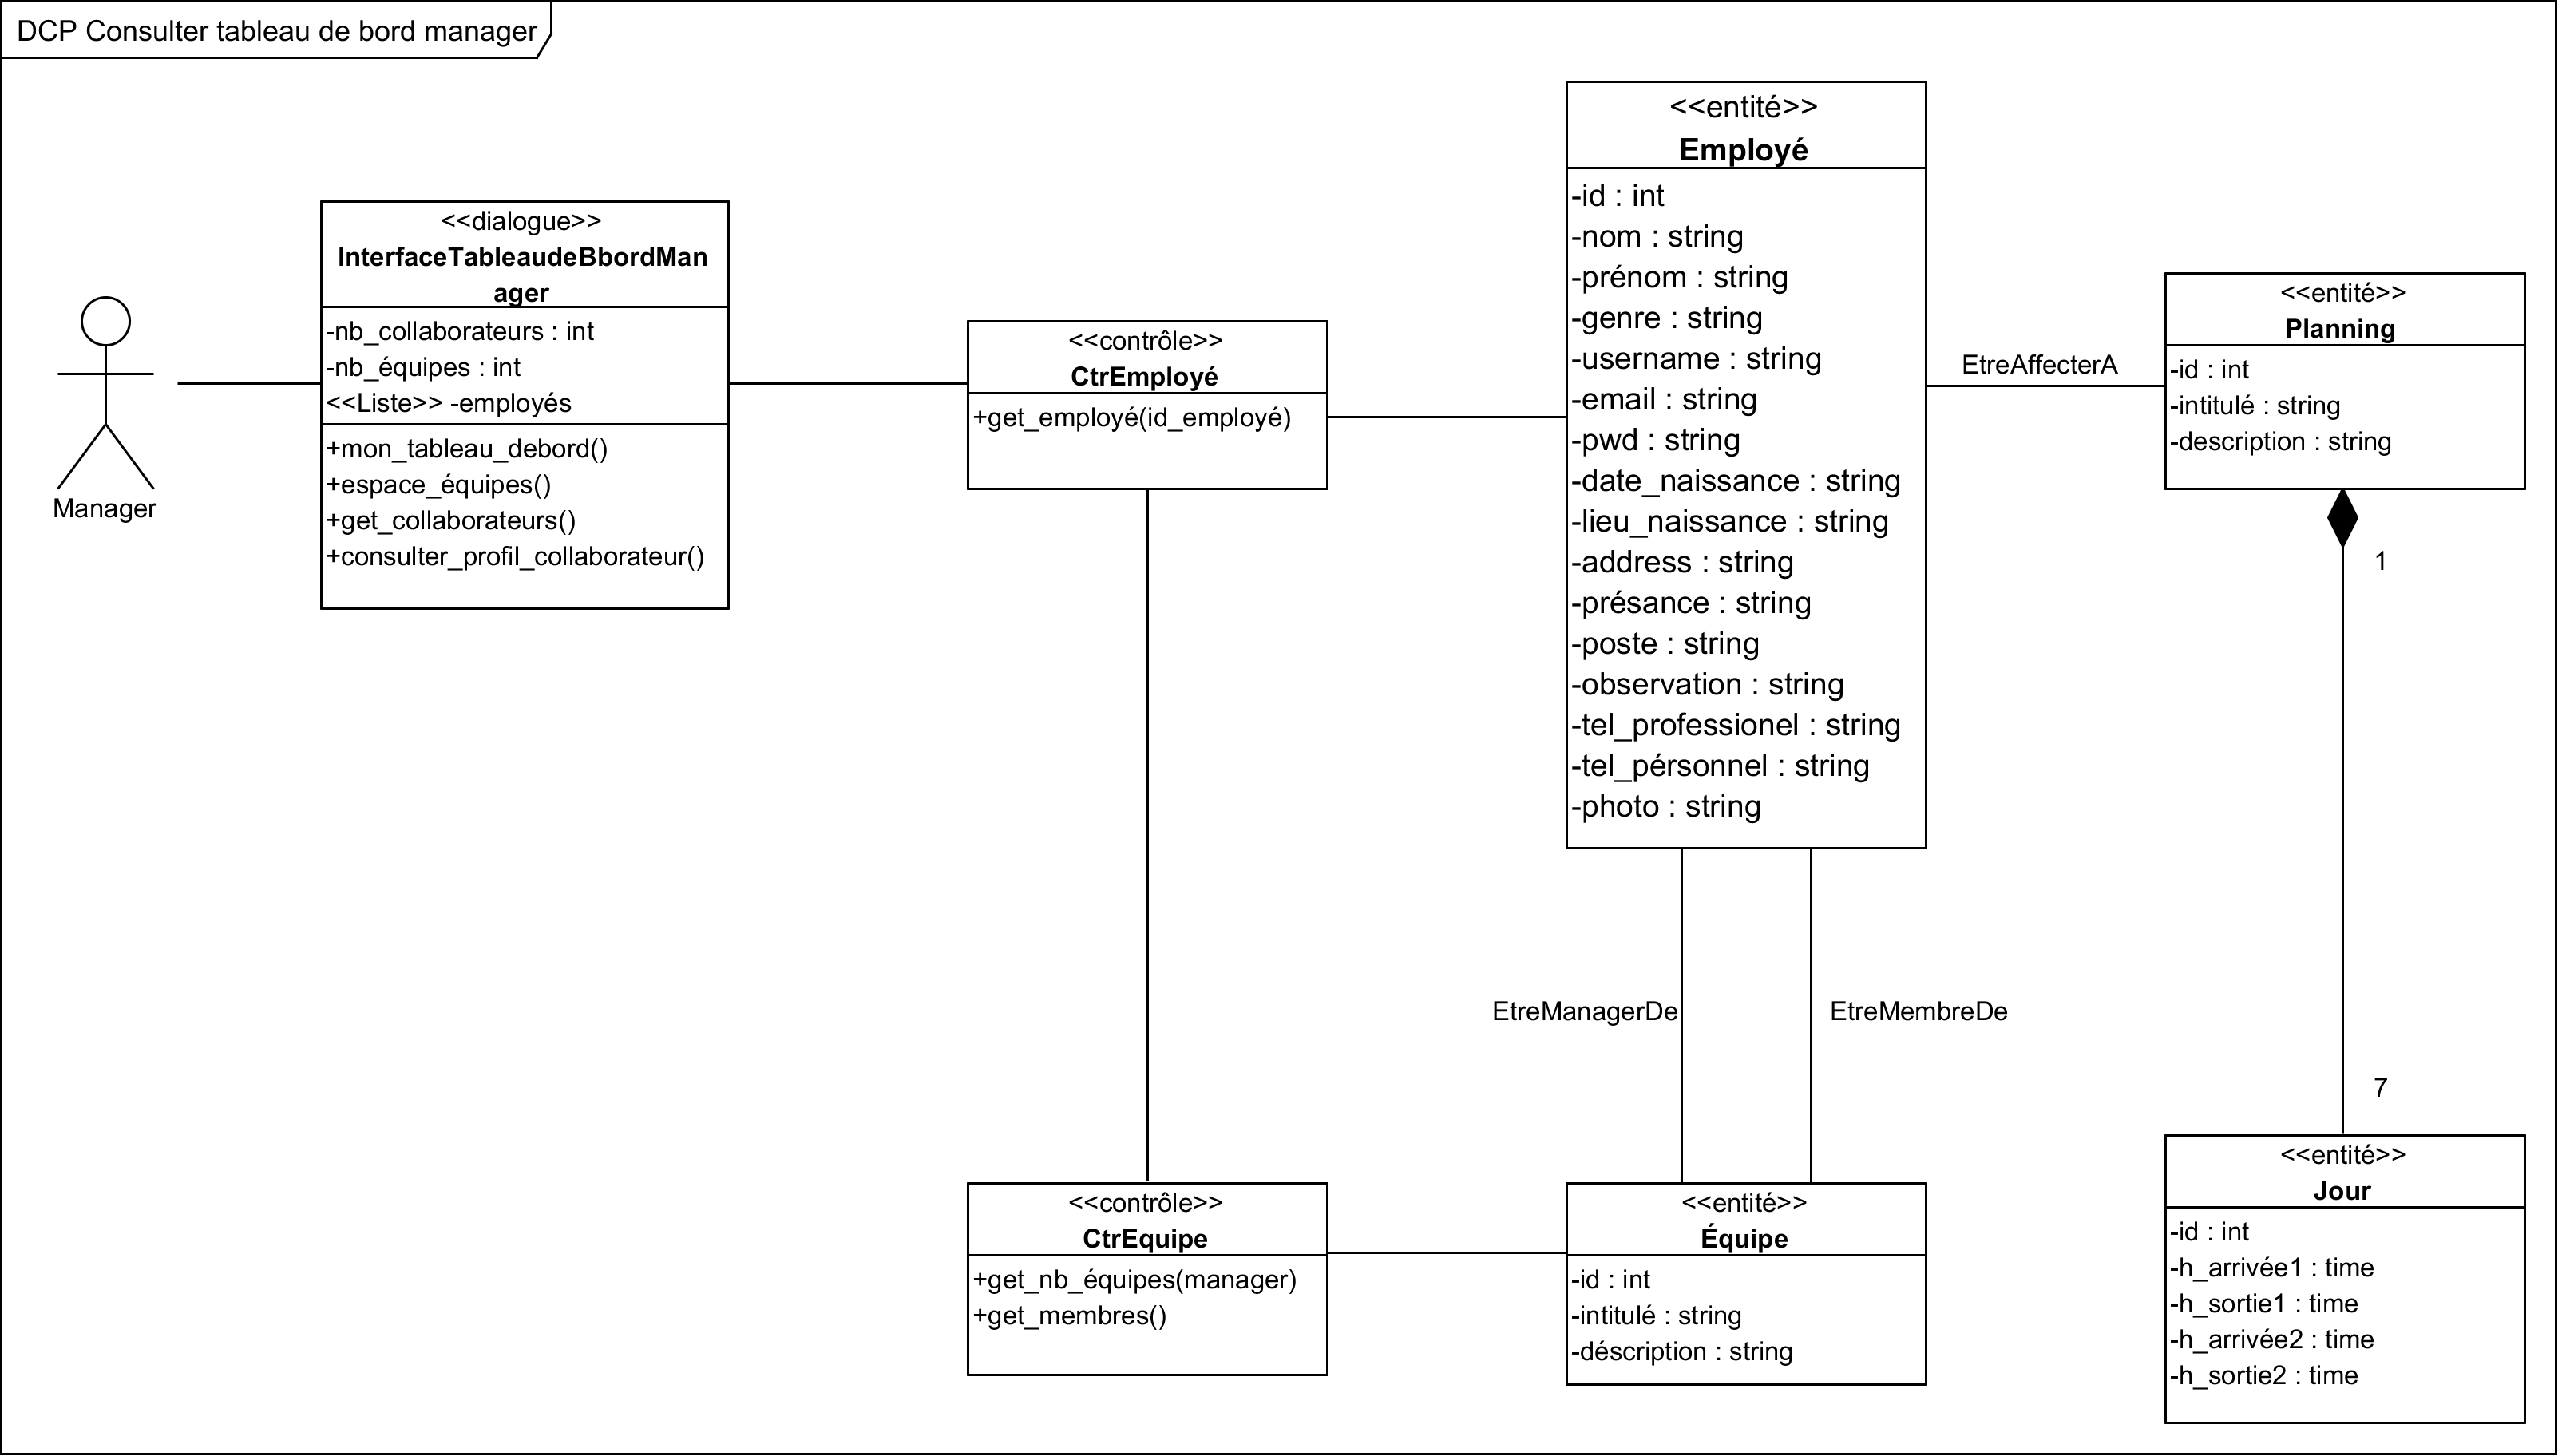
\includegraphics[scale=0.68,angle=90]{images/DCP/DCP Consulter tableau de bord manager.png}
    \caption{Diagrammes de classes participantes « Consulter tableau de bord manager »}
    \label{fig27}
    \end{figure}

\clearpage
       
\subsection*{Diagrammes de classes participantes du cas d'utilisation « Ajouter planning »}
L’interface « InterfaceAjouterPlanning » affiche un formulaire qui permet à
l’acteur de créer un nouveau planning. Il doit saisir le nom, la description,
ainsi que les différents horaires de travail. Une fois validé par l’acteur,
CtrPlanning vérifie les informations saisies pour enfin pouvoir ajouter le
planning à son entité correspondante.
           
\begin{figure}[h!]
    \centering
    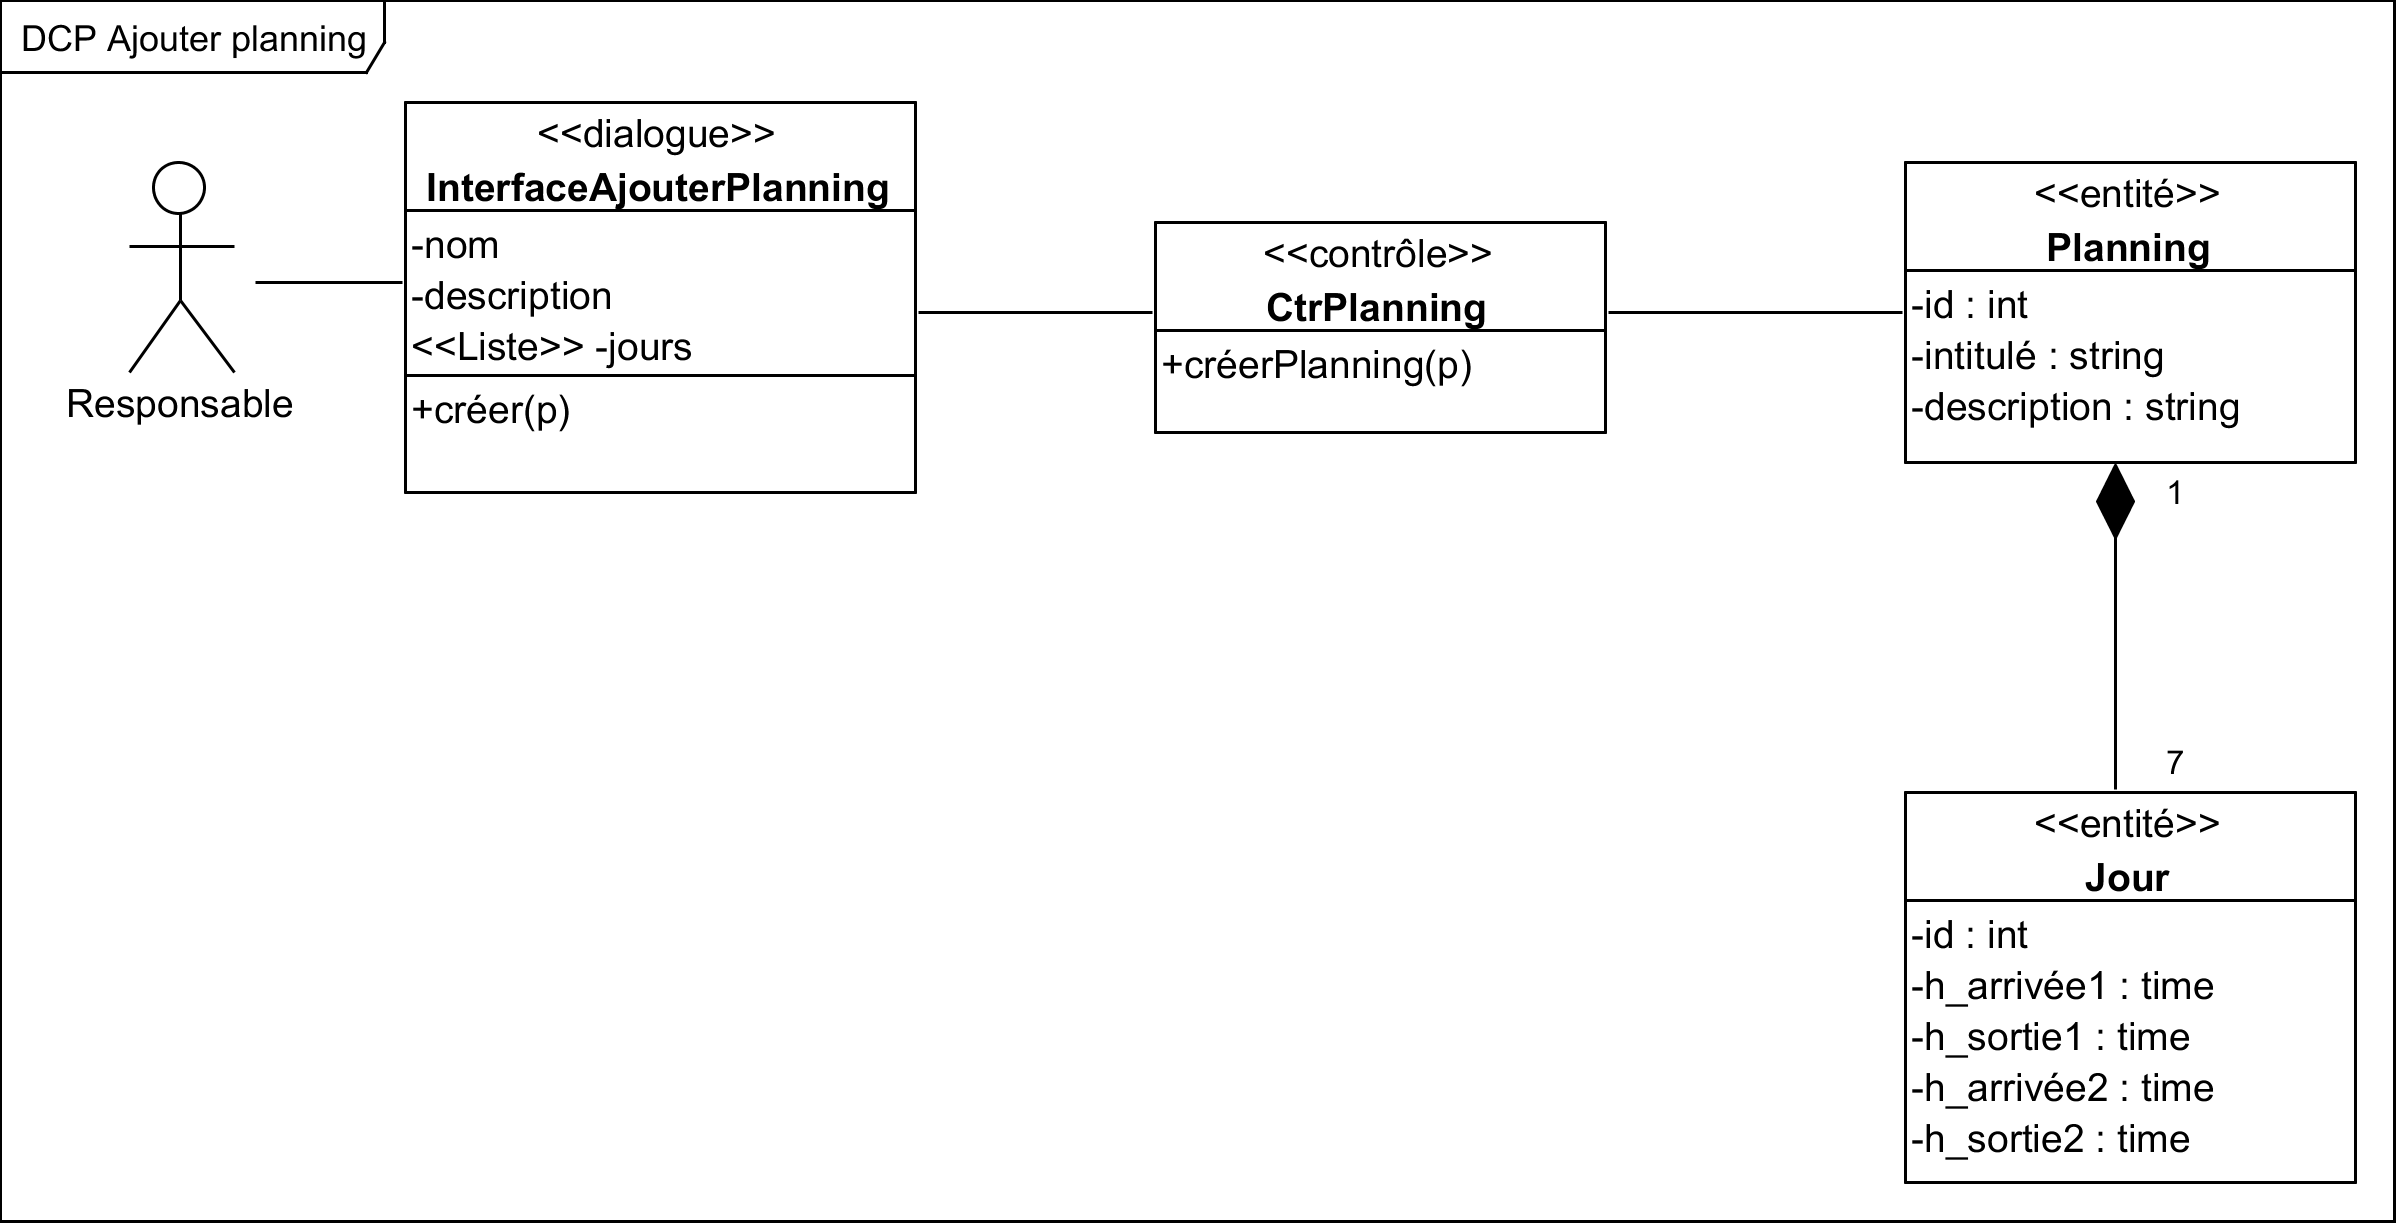
\includegraphics[scale=0.88]{images/DCP/DCP Ajouter planning.png}
    \caption{Diagrammes de classes participantes « Ajouter planning »}
    \label{fig28}
\end{figure}
        
\subsection*{Diagrammes de classes participantes du cas d'utilisation « Ajouter équipe »}
L’interface « InterfaceAjouterEquipe » affiche un formulaire qui permet à
l’acteur de créer une nouvelle équipe. Il doit saisir le nom, la description
ainsi que chercher et sélectionner un manager qui sera le responsable de cette
dernière.
        
La logique concernant les actions effectuées par l’acteur est déléguée à 
deux contrôleurs, CtrEmployé qui va gérer la recherche du manager et CtrEquipe
qui vérifiera les informations saisies pour pouvoir ajouter l’équipe à son 
entité correspondante.
       
\clearpage
            
\begin{figure}[h!]
    \centering
    \includegraphics[scale=0.85]{images/DCP/DCP Ajouter équipe.png}
    \caption{Diagrammes de classes participantes « Ajouter équipe »}
    \label{fig29}
\end{figure}
            
\subsection*{Diagrammes de classes participantes du cas d'utilisation « Ajouter membre »}
L’interface « InterfaceAjouterMembre » affiche à l’acteur une liste des membres 
de l’équipe, ainsi qu’un champ qui lui permettra de faire une recherche d’un 
employé afin de l’ajouter à l’équipe.
        
Pour ce qui est des classes de contrôles, la première classe CtrEquipe aura la 
responsabilité de gérer la recherche, et l’ajout des membres de l’équipe. Quant
à la deuxième classe CtrAffectation, elle permettra de créer une affectation pour 
chaque employé ajouter.
       
\clearpage
            
\begin{figure}[h!]
	\centering
    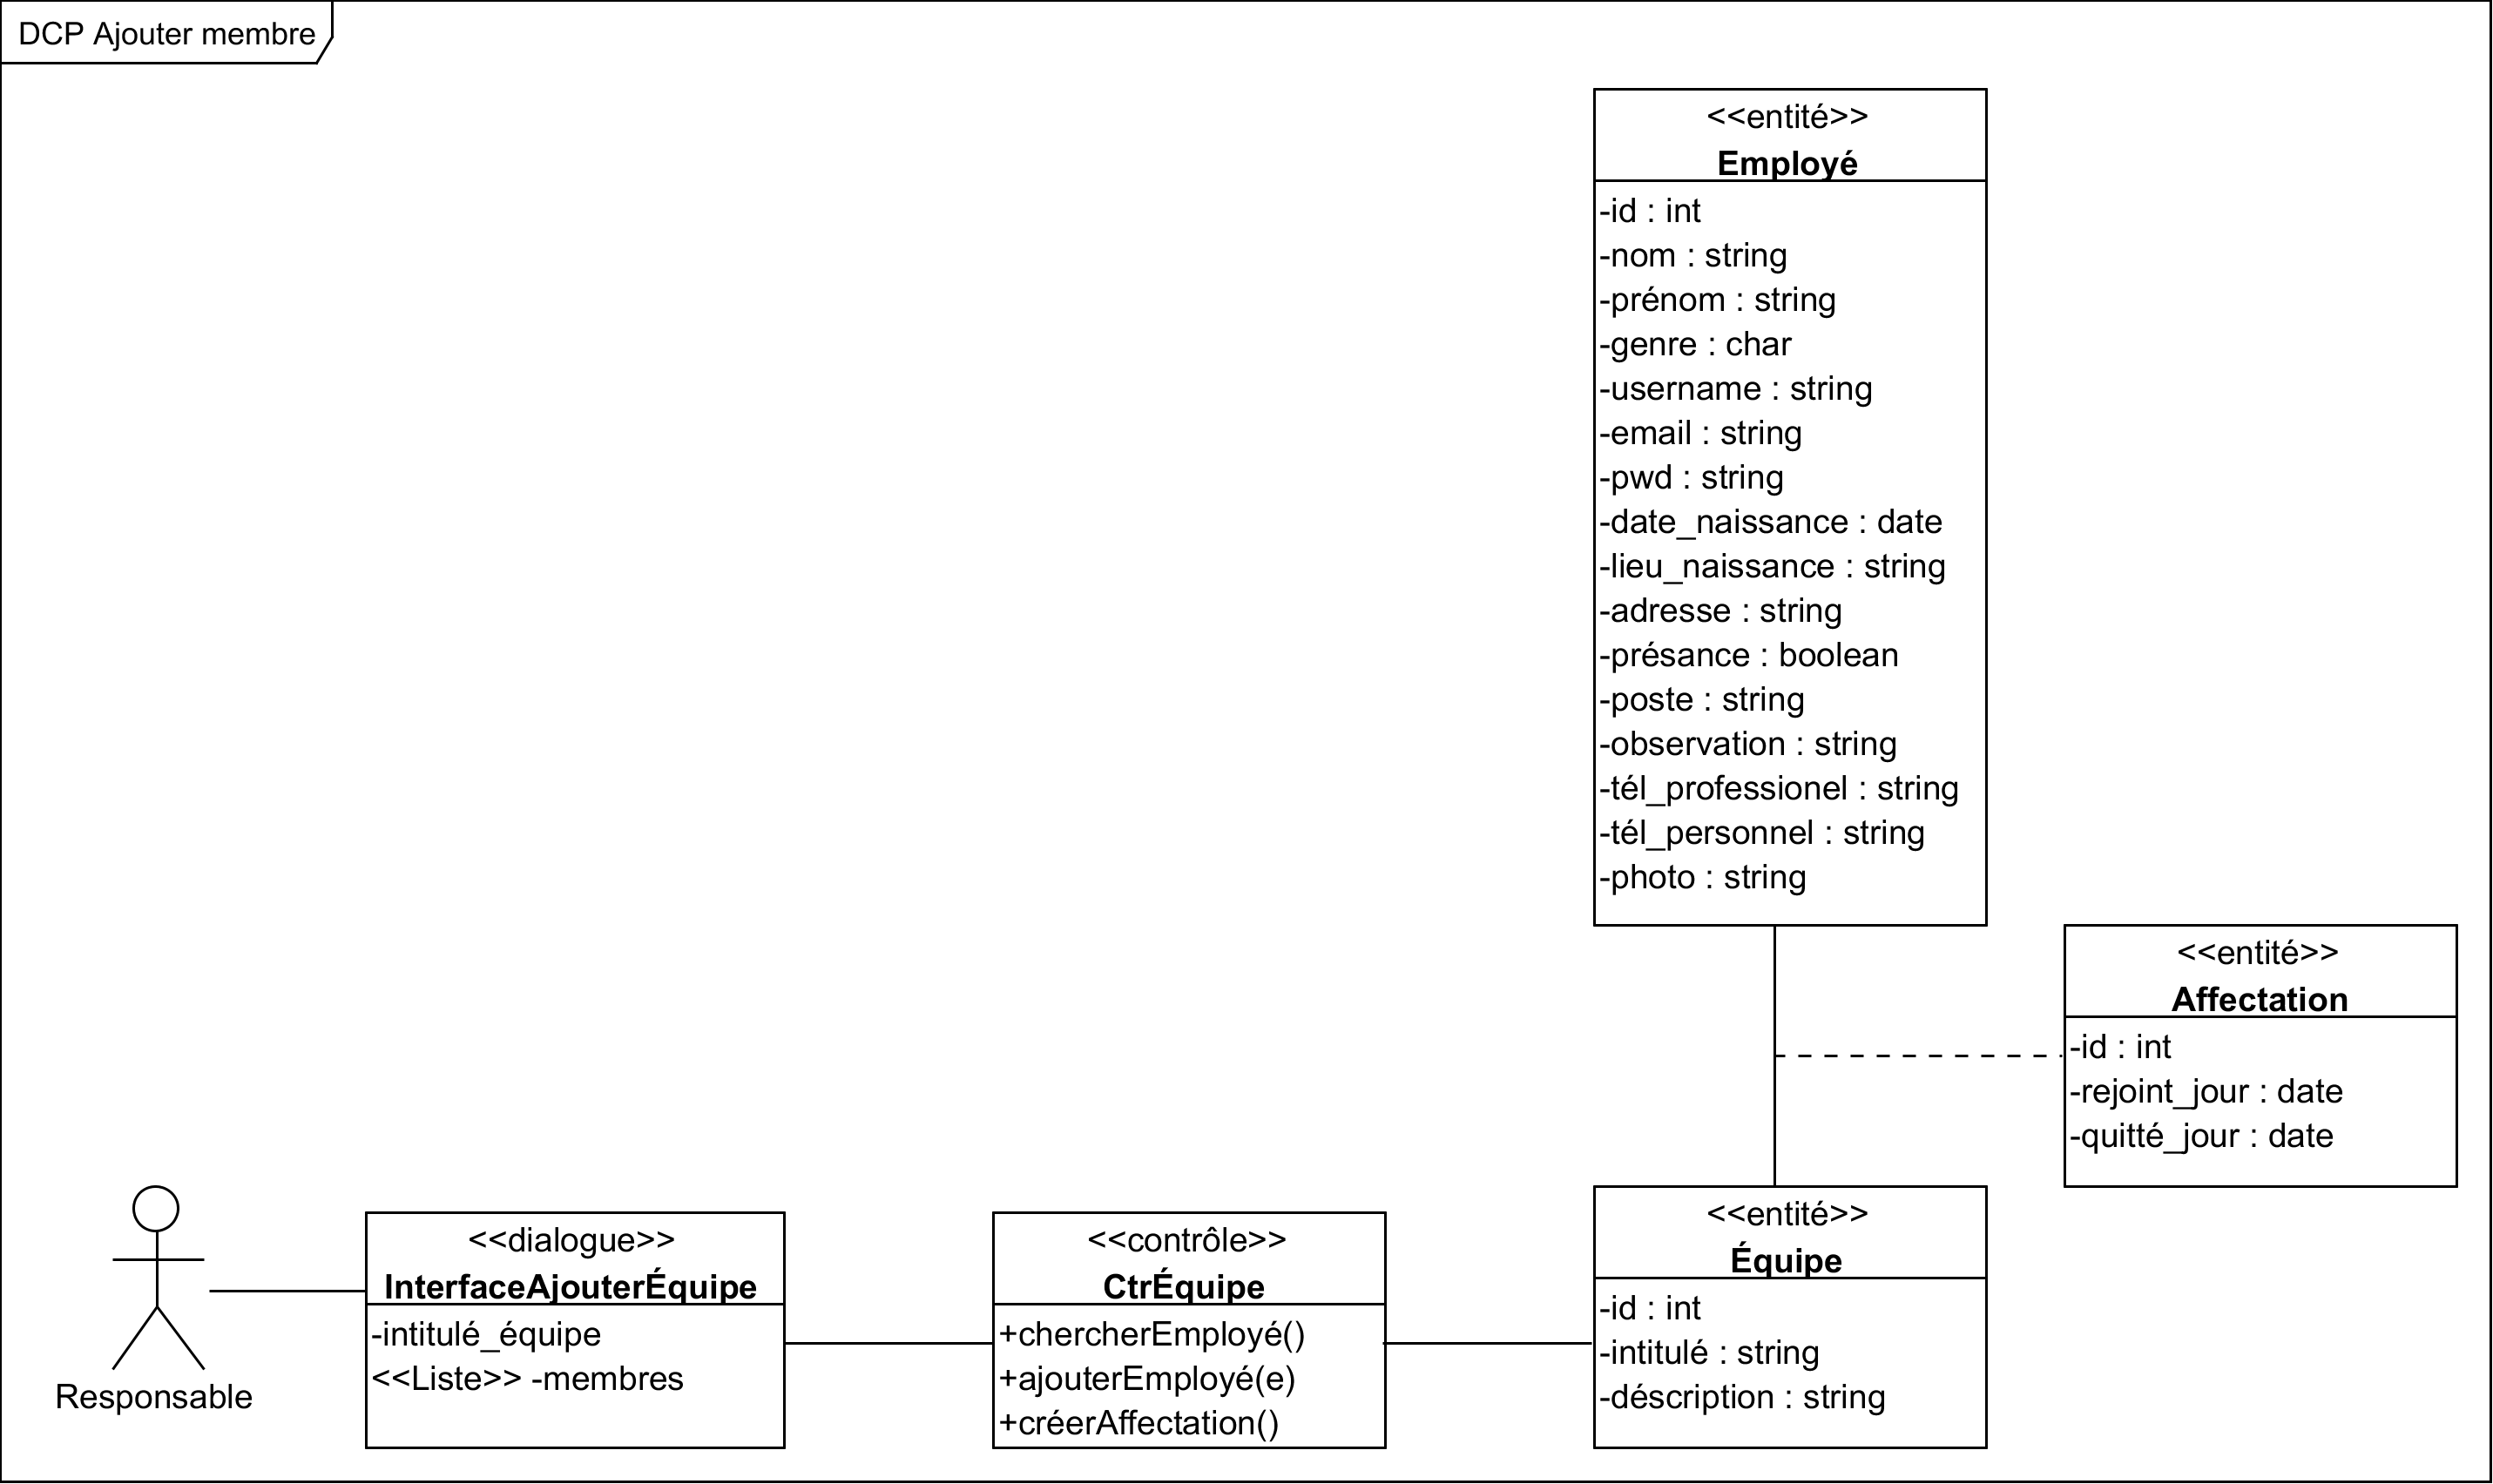
\includegraphics[scale=0.72]{images/DCP/DCP Ajouter membre.png}
    \caption{Diagrammes de classes participantes « Ajouter membre »}
    \label{fig30}
\end{figure}
            
\subsection*{Diagrammes de classes participantes du cas d'utilisation « Ajouter employé »}
L’administrateur à travers l’interface « InterfaceAjouterEmployé » peut ajouter
un employé en remplissant le formulaire. Après avoir validé, l’administrateur
devra ajouter l’empreinte de l’employé qui sera gérée par la classe
CtrEmpreinte.  Une fois enregistrée, la classe CtrEmployé récupèrera l’empreinte
pour finaliser l’enregistrement de l’employé. 

\clearpage

\begin{figure}[h!]
    \centering
    \includegraphics[scale=0.7]{images/DCP/DCP Ajouter employé.png}
    \caption{Diagrammes de classes participantes « Ajouter employé »}
    \label{fig31}
\end{figure}
        
\subsection*{Diagrammes de classes participantes du cas d'utilisation « Consulter profil d'un employé »}
L’interface « InterfaceConsulterProfilEmployé » permet au responsable de 
consulter le profil d’un employé où il aura accès à toutes ses informations. Il 
pourra aussi à partir de cette interface accéder à l’interface de modification
du profil et du planning de l’employé. Quant à la classe CtrEmployé, elle permet 
de récupérer l’employé sélectionner. 

\begin{figure}[h!]
    \centering
    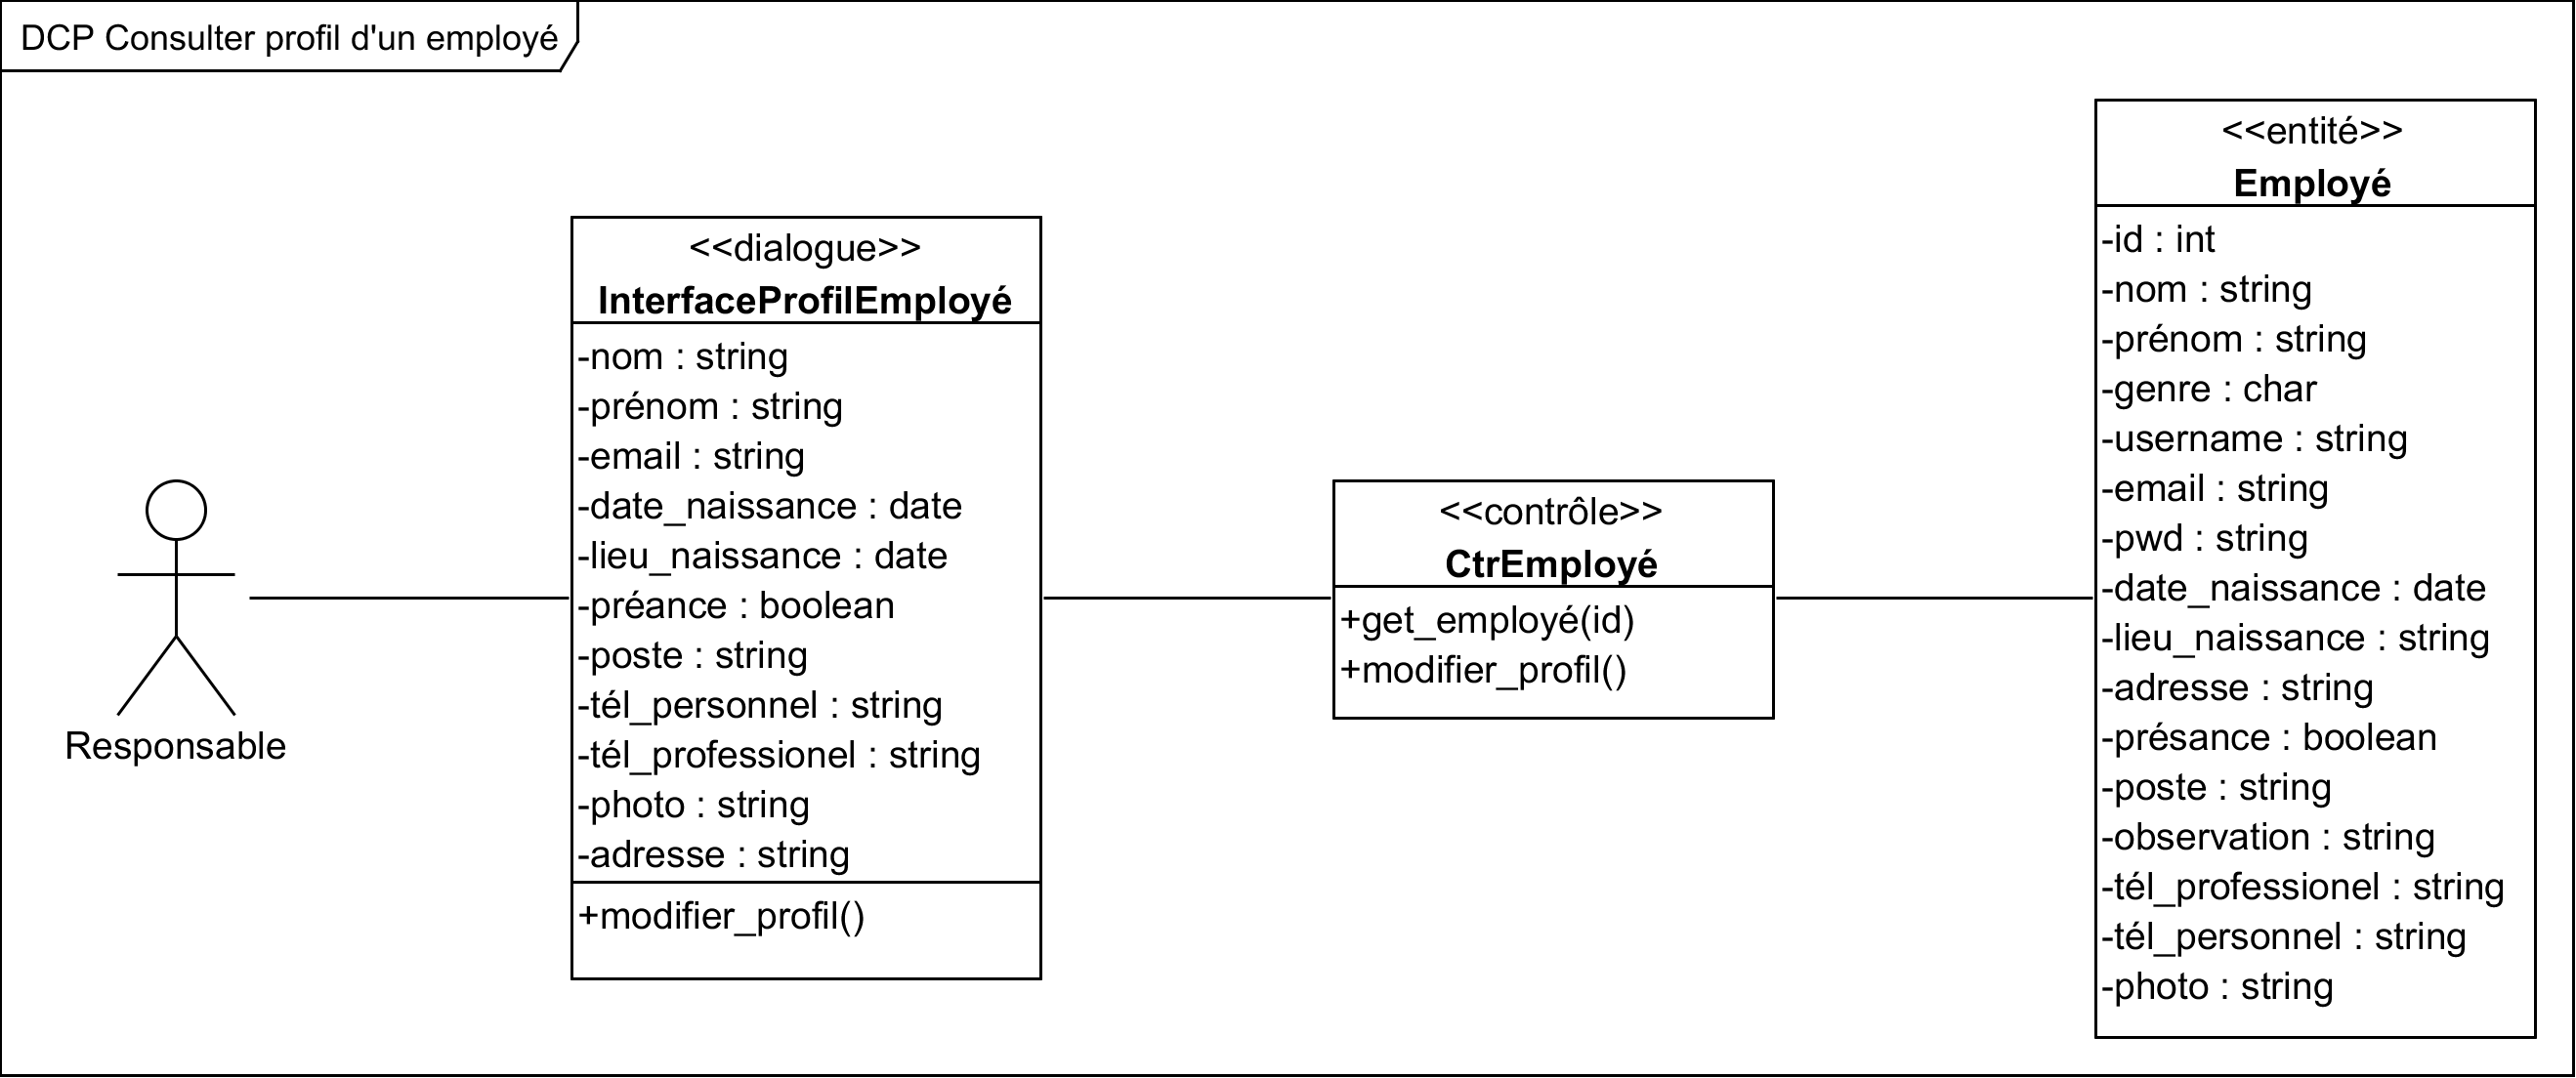
\includegraphics[scale=0.72]{images/DCP/DCP_consulter_profil_d'un_employe.png}
    \caption{Diagrammes de classes participantes « Consulter profil employé »}
    \label{fig32}
\end{figure}
             
\section{Diagrammes de séquence}
L’objectif du diagramme de séquence est de représenter les interactions entre 
objets en indiquant la chronologie des échanges. Cette représentation peut se 
réaliser par cas d’utilisation en considérant les différents scénarios 
associés.\cite{9} 
    
Dans cette partie, nous allons détailler les diagrammes de séquence système 
élaborés dans le chapitre 2, en remplaçant le système vu comme une boîte 
noire par un ensemble d’objets de classes différentes tout en respectant 
les règles suivantes:

\begin{itemize}
        \item[\textbullet] Les acteurs ne peuvent interagir (envoyer des messages) 
            qu’avec les dialogues.
        \item[\textbullet] Les dialogues peuvent interagir avec les contrôles. 
        \item[\textbullet] Les contrôles peuvent interagir avec les dialogues, les 
            entités, ou d’autres contrôles.
        \item[\textbullet] Les entités ne peuvent interagir qu’entre elles.             
\end{itemize}

Le formalisme est donné dans l’exemple type présenté à la figure \ref{fig33}\\

\begin{figure}[h!]
    \centering                 
    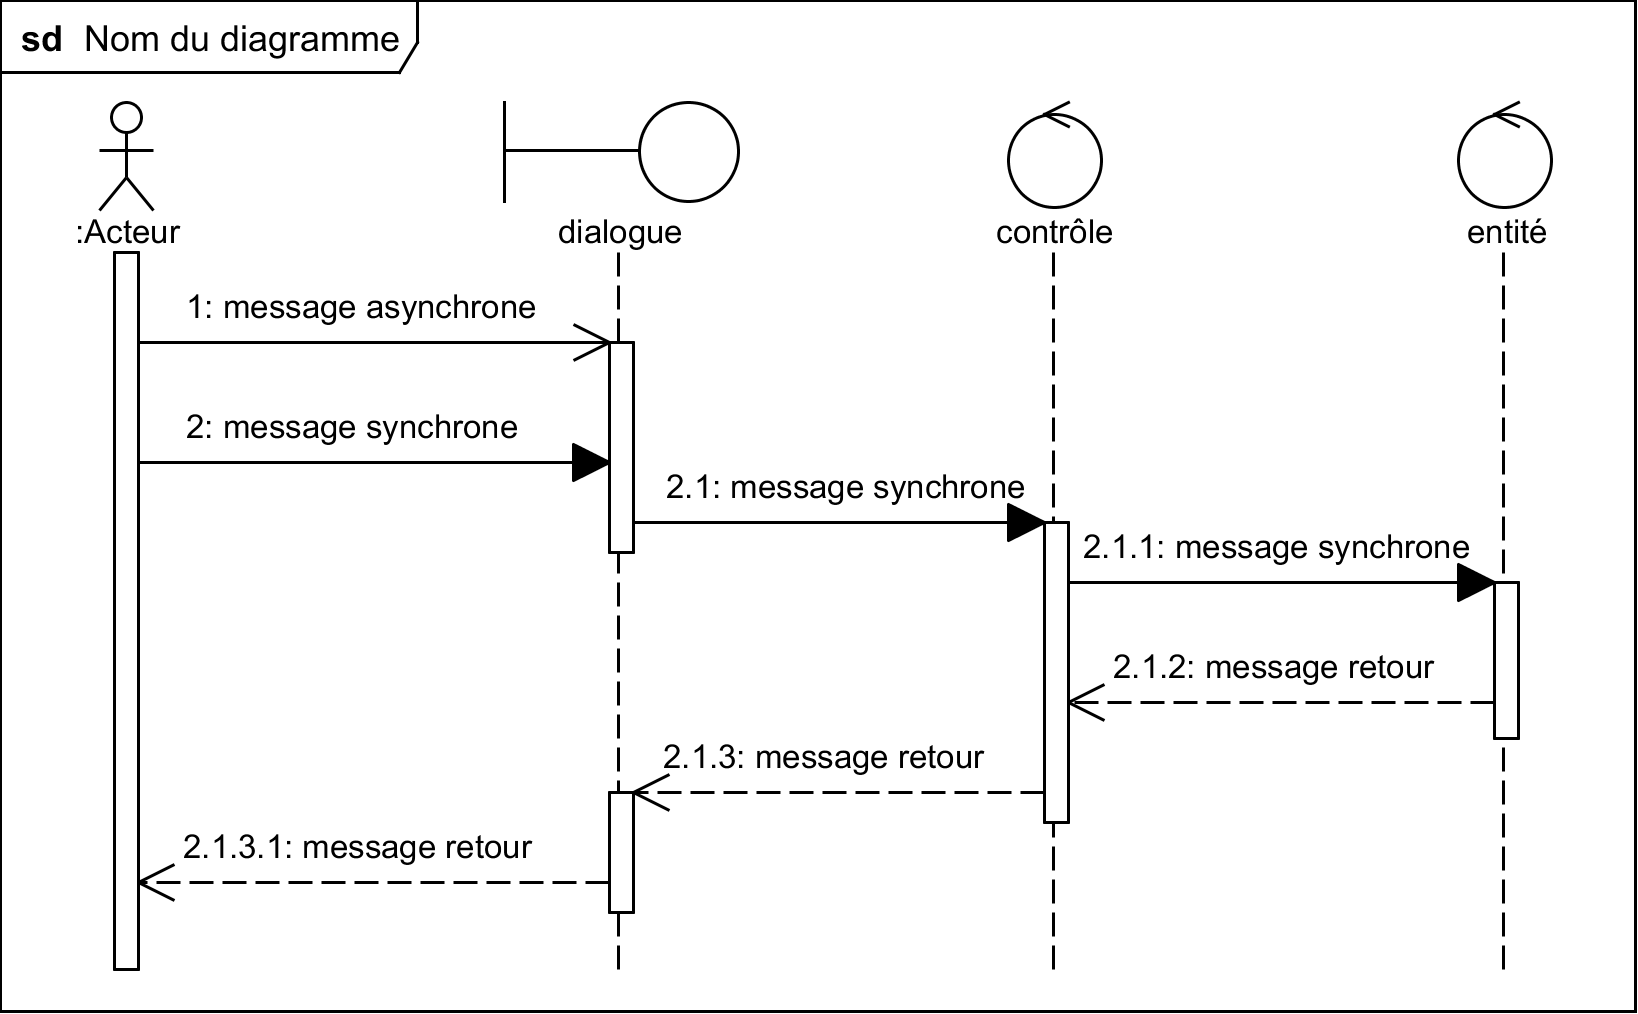
\includegraphics[scale=1.23]{images/exemple ds.png}
    \caption{Formalisme du diagramme de séquence}
    \label{fig33}
\end{figure}

\clearpage
    
\subsection*{Diagramme d'interaction du cas d'utilisation « Se pointer »}
Avant chaque entrée ou sortie de l’entreprise, l’employé doit se pointer avec son 
empreinte digitale afin que la pointeuse l’identifie. Après une courte 
vérification, si l’empreinte n’est pas reconnue aucune LED ne s’allume, par 
contre si la pointeuse la reconnait, elle signale au contrôle CtrEmployé qui 
récupère son identifiant, puis délègue au contrôle CtrShift la recherche de son 
dernier pointage et la vérification du type de pointage. Une fois effectué, le 
contrôle CtrEmployé déclenche l’enregistrement du pointage, si le type de 
pointage est une sortie alors le contrôle CtrShift insérera l’heure de sortie 
dans le dernier pointage, si c’est une entrée alors un nouveau pointage est 
créé avec l’heure d’entrée et l’identifiant de l’employé.

\begin{figure}[h!]
    \centering
    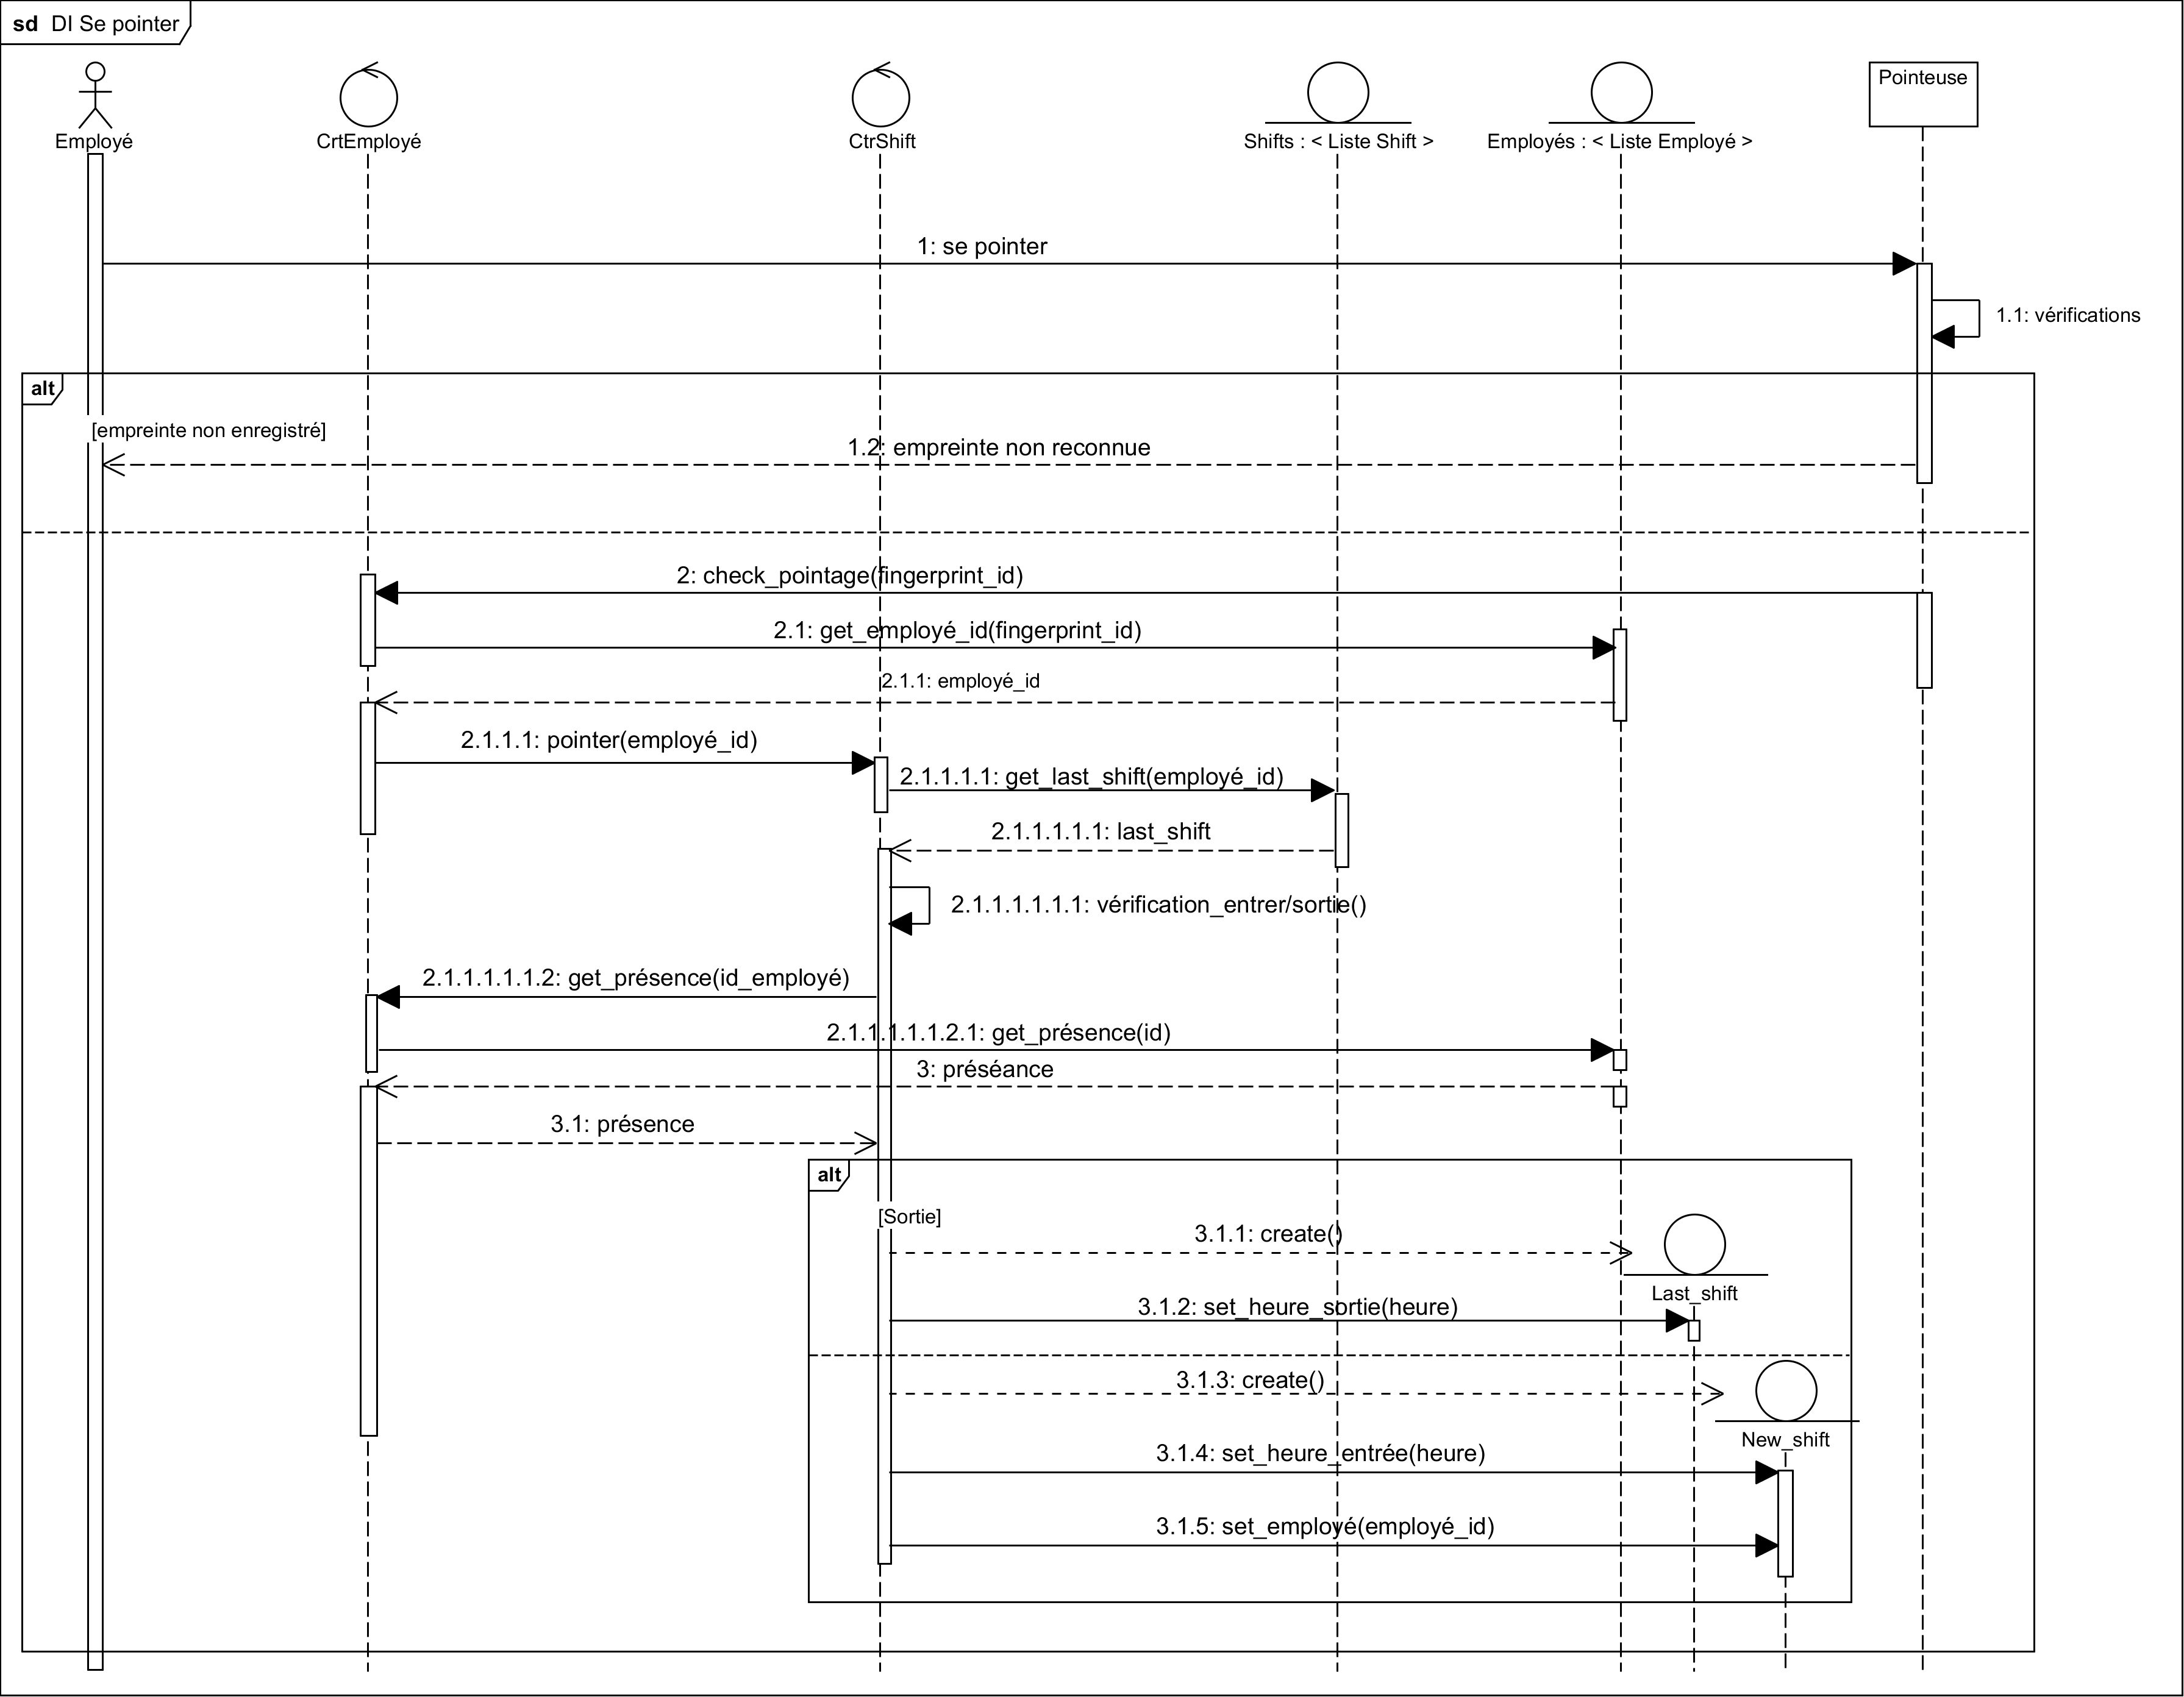
\includegraphics[scale=0.56]{images/DS/DI Se pointer.png}
    \caption{Diagramme d'interaction « Se pointer »}
    \label{fig34}
\end{figure}
        
\clearpage
    
\subsection*{Diagramme d'interaction du cas d'utilisation « Consulter mon profil »}
Une fois authentifié, l’employé peut consulter son profil à travers n’importe 
quelle interface, il est redirigé vers l’interface MonProfil qui délègue la 
recherche avec l’identifiant au contrôle CtrEmployé. Une fois la recherche 
effectuée, les informations sont affichées. Il pourra aussi à travers cette 
interface modifier son profil. Une fois les informations saisies, il doit 
valider ce qui déclenchera une vérification, si les informations saisies sont 
correctes les modifications seront enregistrées. Dans le cas contraire, un 
message d’erreur sera affiché.

\begin{figure}[h!]
    \centering
    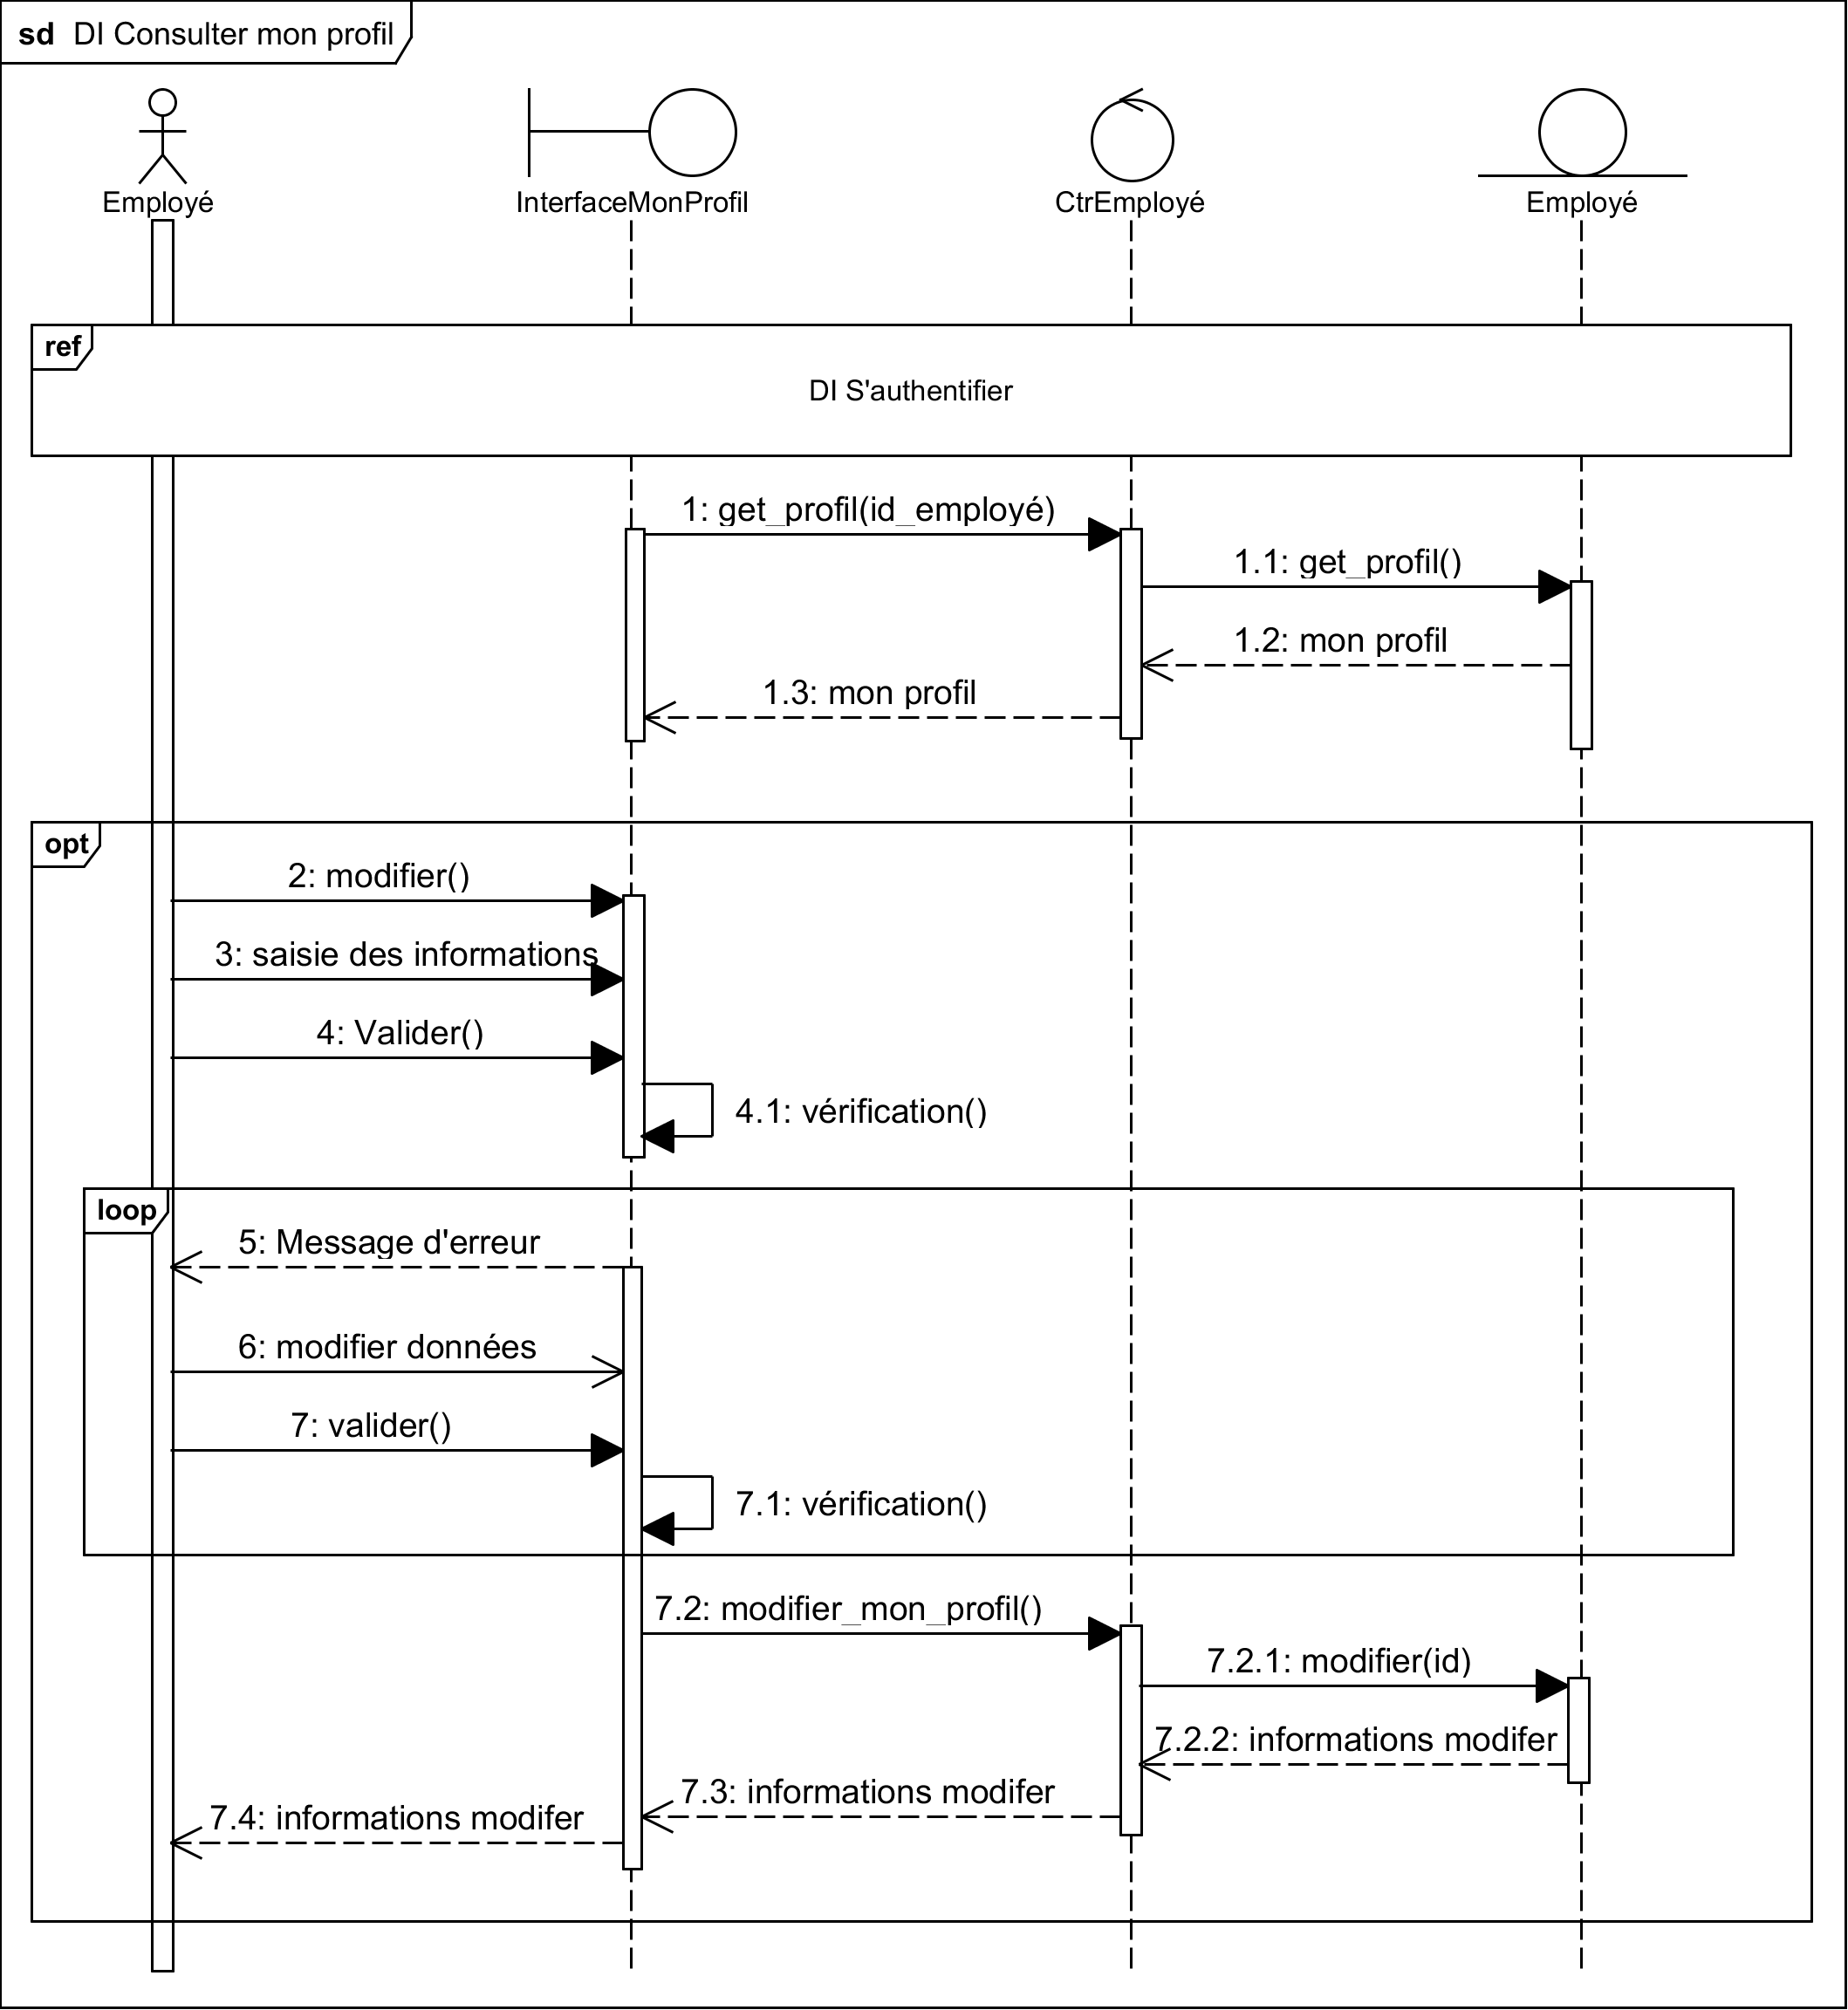
\includegraphics[scale=0.86]{images/DS/consulter_mon_profile}
    \caption{Diagramme d'interaction « Consulter mon profil »}
    \label{fig35}
\end{figure}

\clearpage
    
\subsection*{Diagramme d'interaction du cas d'utilisation « Consulter ma fiche de pointage »}
L’employé devra s’authentifier pour consulter sa fiche de pointage. L’interface 
InterfaceMaFicheDePointage déléguera la recherche de la liste des derniers 
pointages au contrôle CtrShift qui seront affichés par semaine. L’employé aura 
aussi la possibilité de les afficher par mois, ainsi que de faire une recherche 
par période. 
        
\begin{figure}[h!]
    \centering
    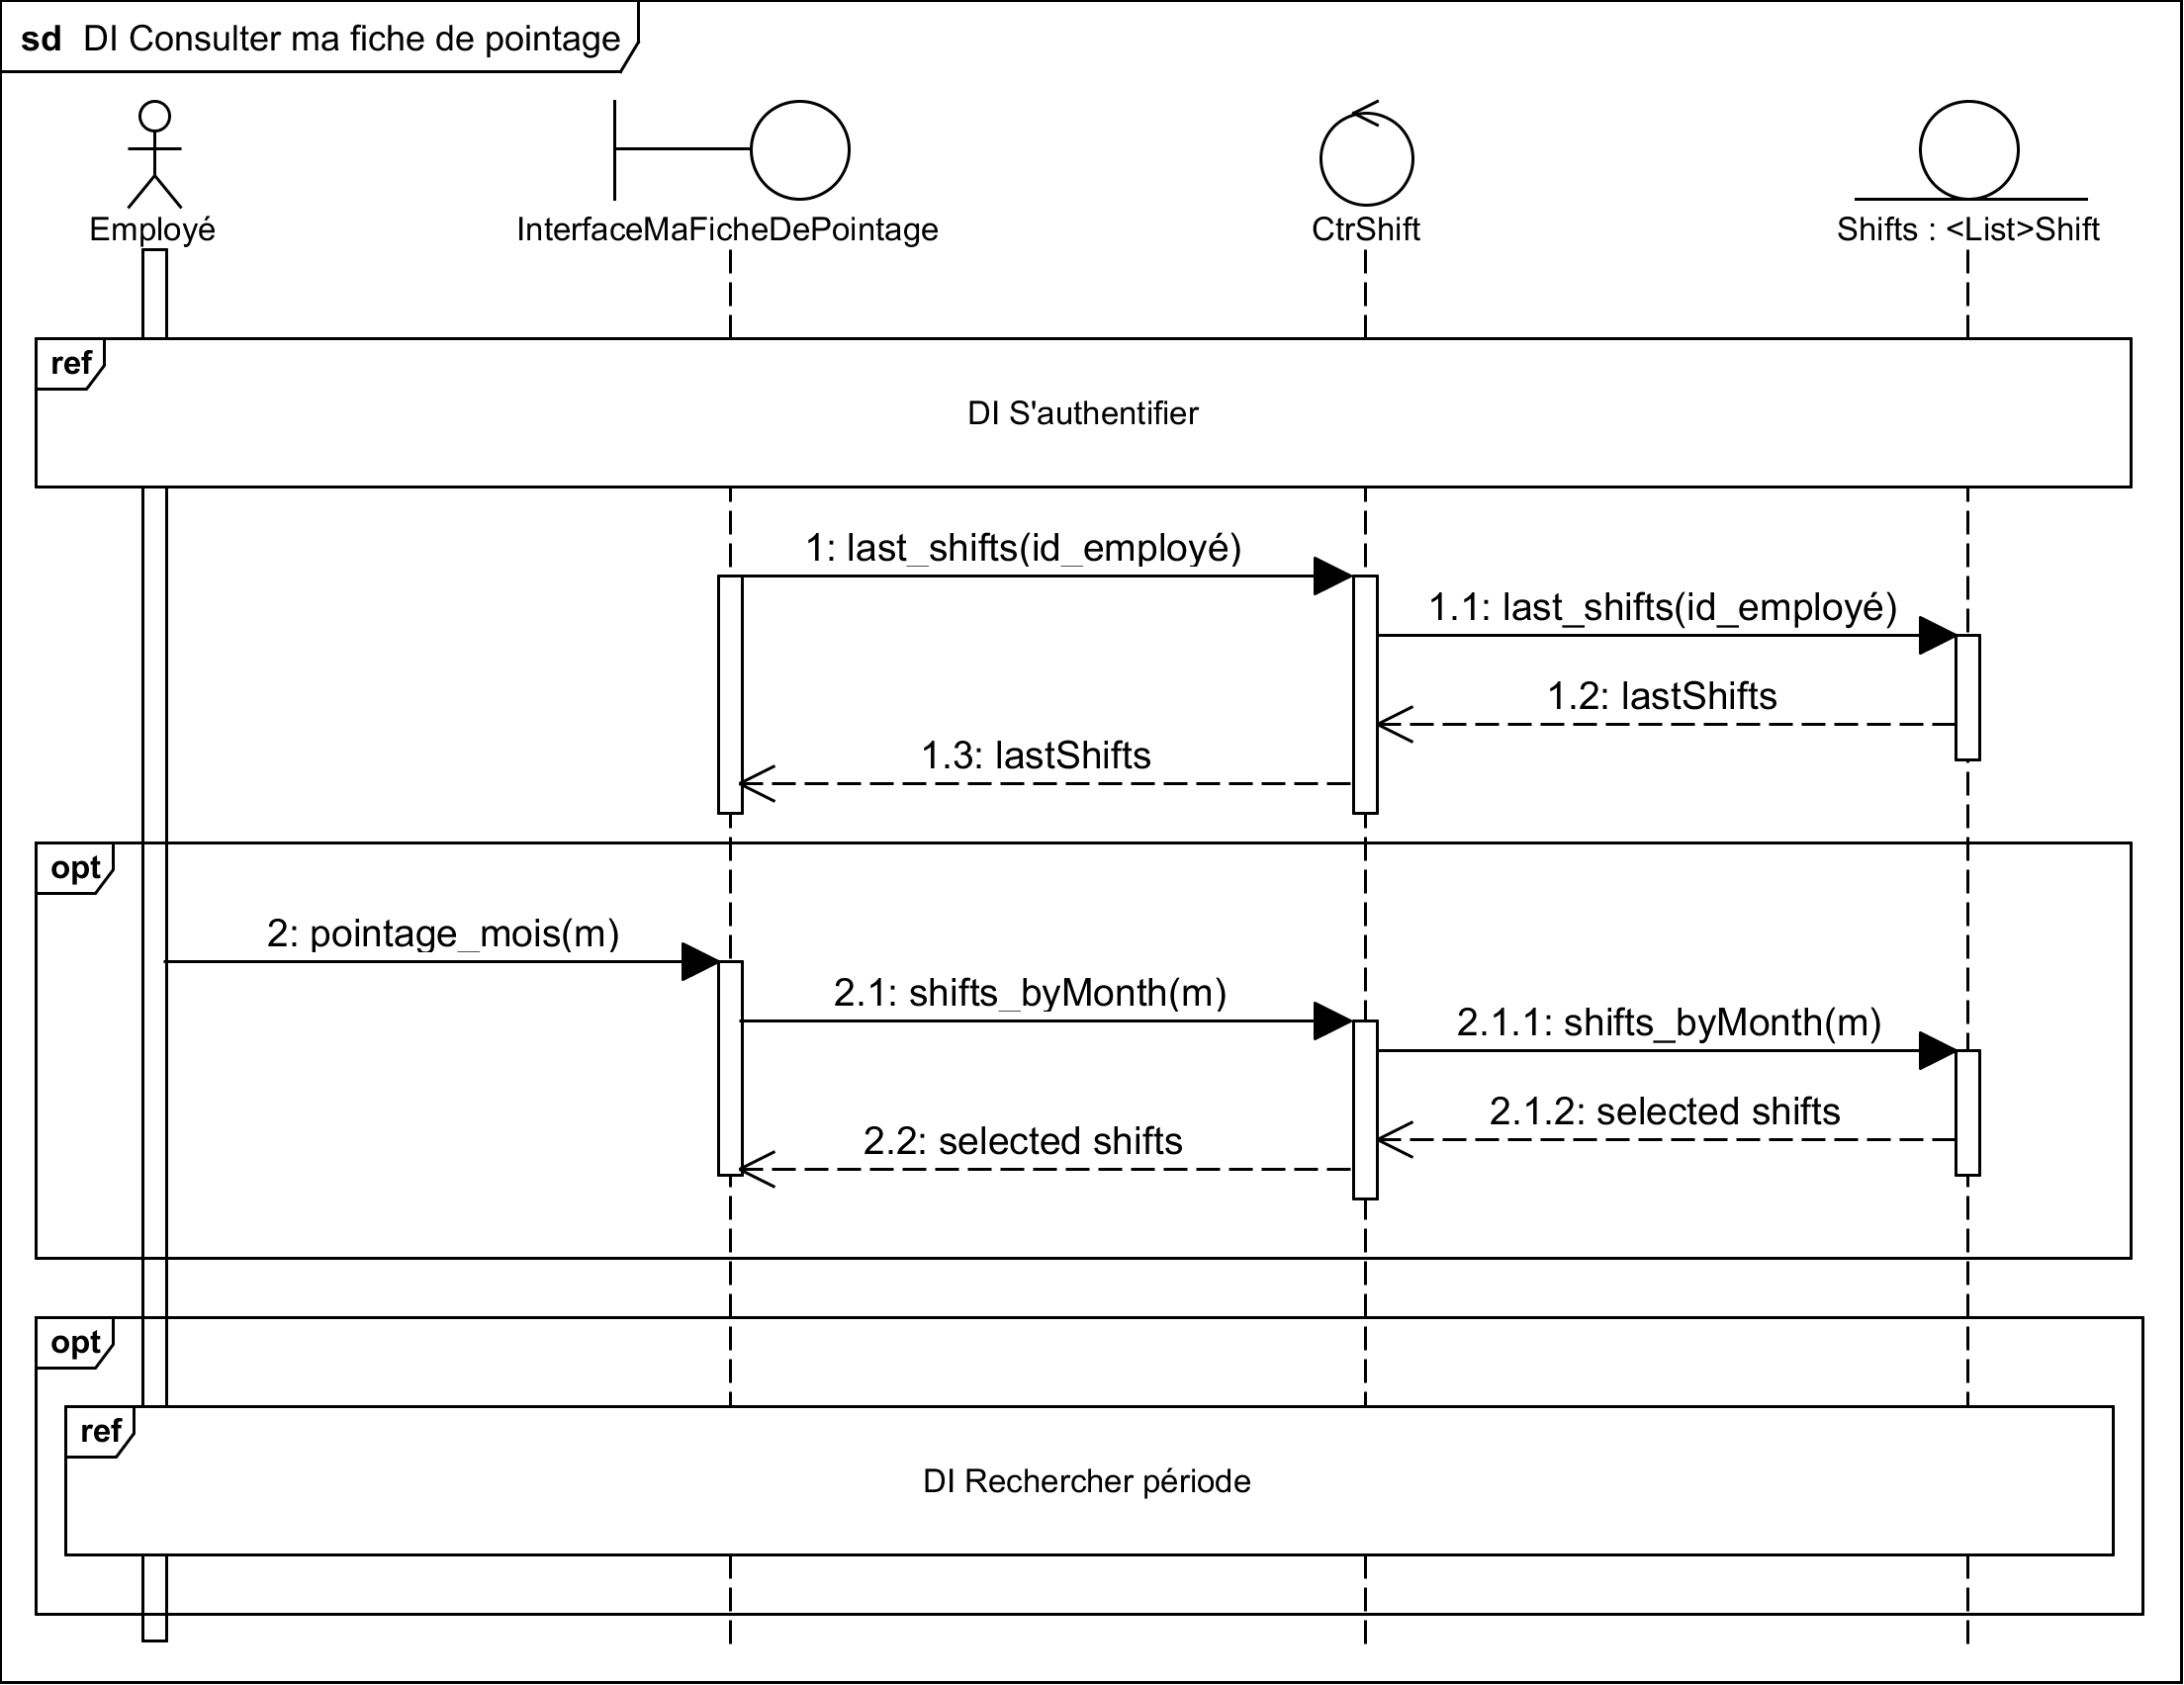
\includegraphics[scale=0.86]{images/DS/DI Consulter ma fiche de pointage.png}
    \caption{Diagramme d'interaction « Consulter ma fiche de pointage »}
    \label{fig36}
\end{figure}    
        
\subsection*{Diagramme d'interaction du cas d'utilisation « Consulter tableau de bord manager »}
Une fois authentifié, le manager est redirigé vers son tableau de bord. En 
premier lieu son espace personnel sera affiché, il pourra sélectionner l’espace 
manager, 3 contrôleurs seront nécessaires, le contrôle CtrEmployé pour récupérer 
la liste de ses collaborateurs, le contrôle CtrEquipe pour récupérer la liste 
des équipes du manager, et le dernier contrôle CtrSHift pour récupérer la liste 
des pointages de ses collaborateurs.

\clearpage

\begin{figure}[h!]
    \centering
    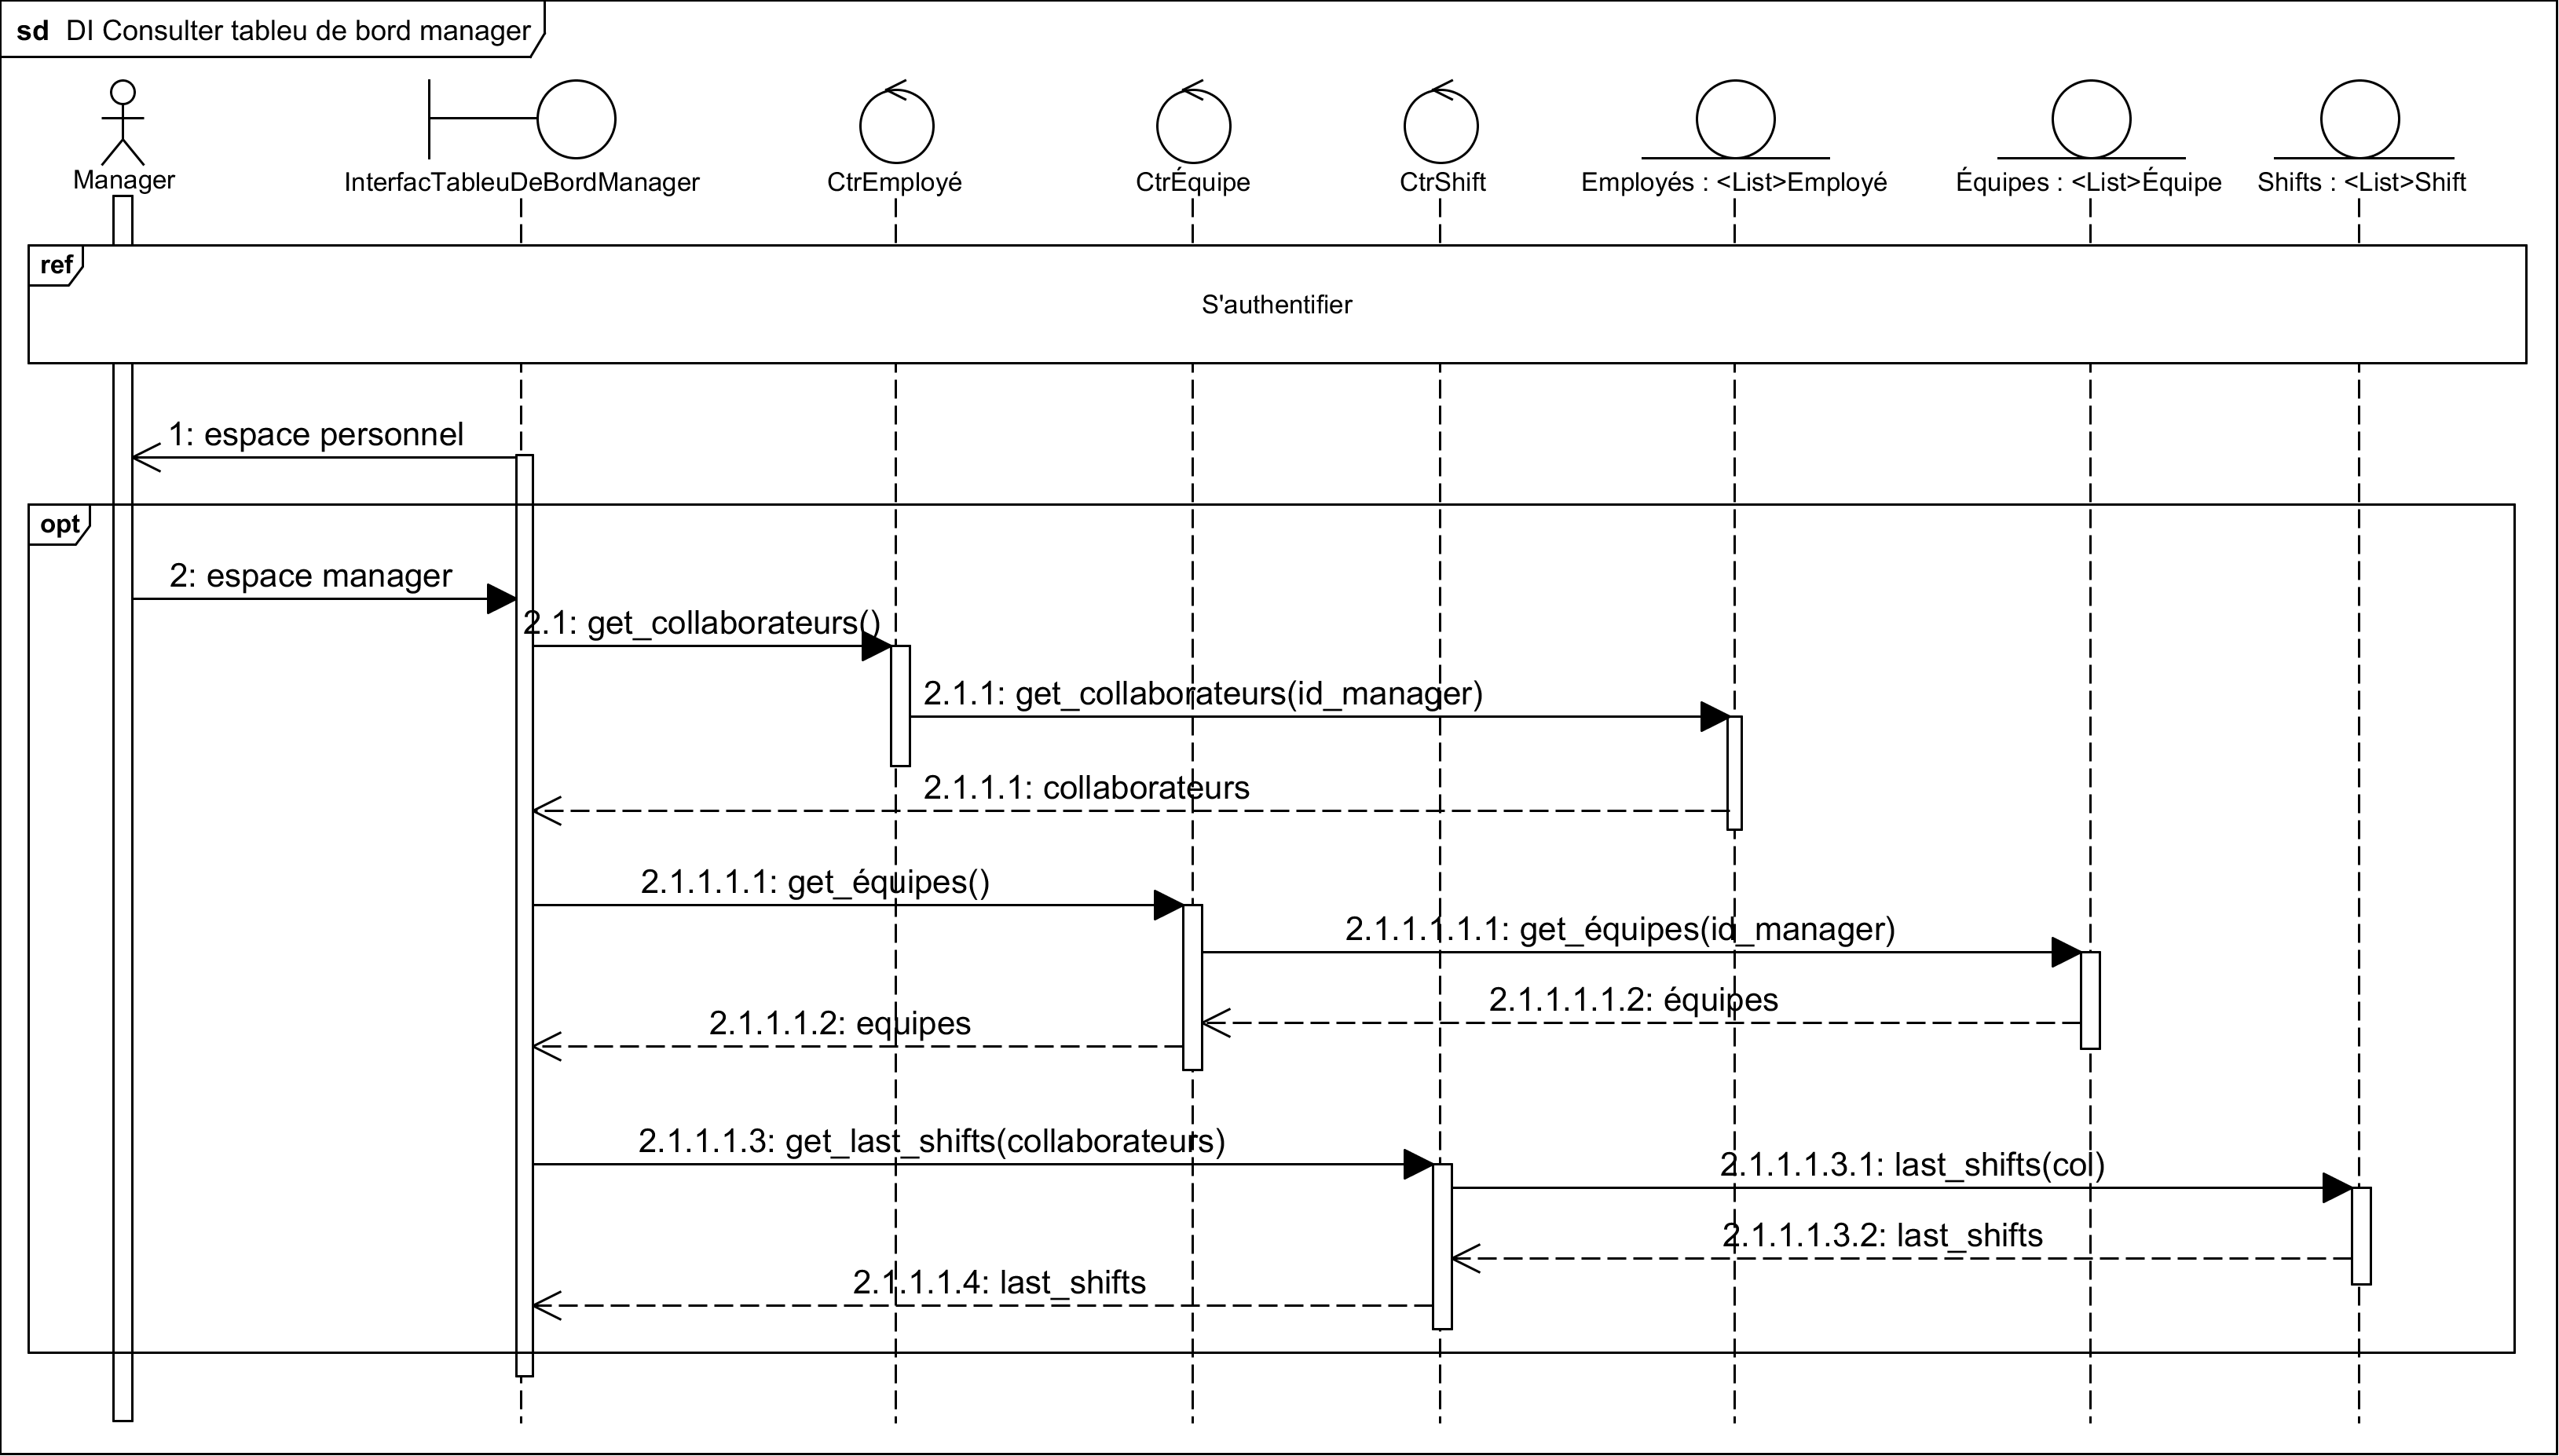
\includegraphics[angle=90,scale=0.65]{images/DS/DI Consulter tableu de bord manager.png}
	\caption{Diagramme d'interaction « Consulter tableau de bord manager »}
    \label{fig37}
\end{figure}
        
\subsection*{Diagramme d'interaction du cas d'utilisation « Ajouter équipe »}
L’acteur pourra ajouter une équipe. Après avoir saisi les informations et
sélectionné un manager, une vérification est effectuée. Si aucune erreur n’est
détectée il pourra l’enregistrer, le contrôle CtrEquipe s’occupera de la
création et il déléguera la recherche du manager au contrôle CtrManager, une
fois terminée, l’interface InterfaceAjouterEquipe est détruite et l’acteur sera
redirigé vers l’interface InterfaceGérerEquipe, où il pourra affecter des
membres.

\clearpage

\begin{figure}[h!]
    \centering
    \includegraphics[scale=0.74]{images/DS/DI Ajouter une équipe.png}
    \caption{Diagramme d'interaction « Ajouter équipe »}
    \label{fig38}
\end{figure}

\subsection*{Diagramme d'interaction du cas d'utilisation « Ajouter planning »}
L’acteur aura la possibilité d’ajouter un planning. Pour ce, il doit saisir les
horaires de travail de la semaine ainsi que l’intitulé et la description du
planning.  Après la validation, une vérification des informations sera
effectuée. Si les données sont invalides un message d’erreur sera affiché et
l’acteur devra les corriger. Si les informations sont valides, le contrôle
CtrPlanning vérifiera si aucun planning n’existe avec l’intitulé saisi afin de
valider l’ajout du planning. Une fois terminé, l’acteur pourra affecter un
planning aux employés.

\clearpage

\begin{figure}[h!]
    \centering
    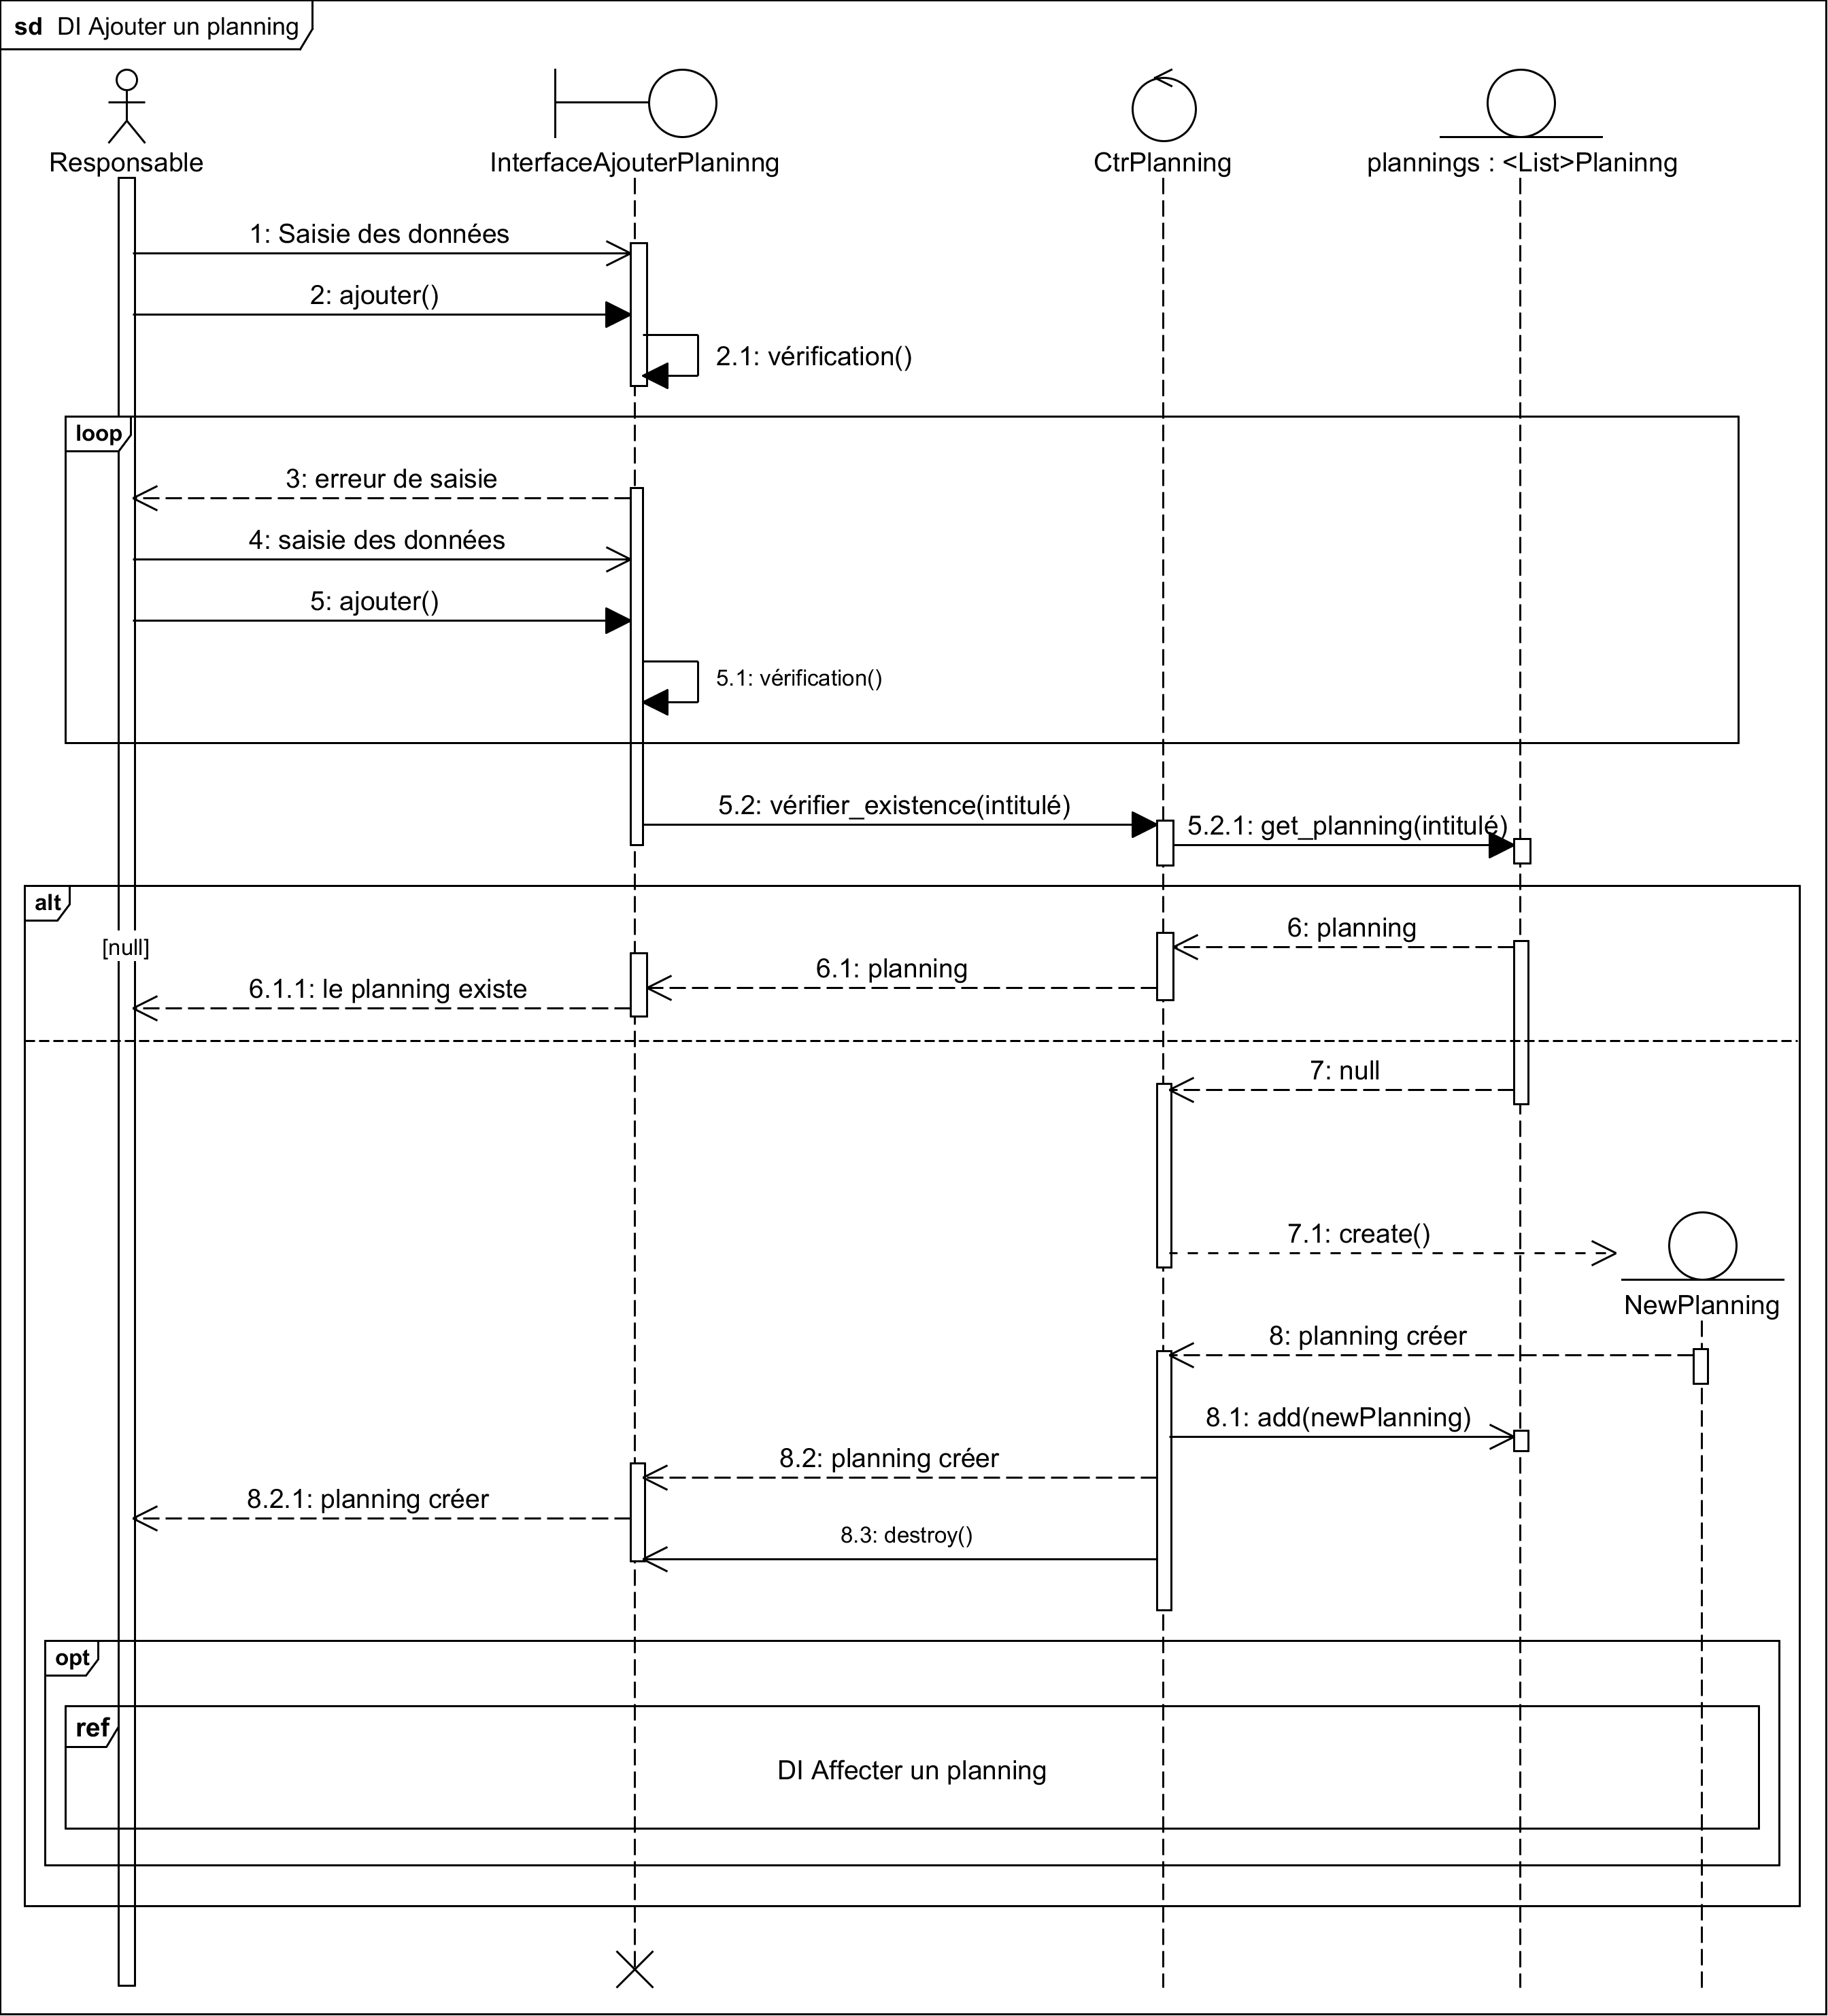
\includegraphics[scale=0.74]{images/DS/DI Ajouter un planning.png}
    \caption{Diagramme d'interaction « Ajouter planning »}
    \label{fig39}
\end{figure}
        
\subsection*{Diagramme d'interaction du cas d'utilisation « Ajouter membre »}
L’acteur aura la possibilité d’ajouter un membre à une équipe, il devra 
effectuer une recherche qui lui permettra à travers l’interface 
InterfaceAjouterMembre d’affecter un employé s’il existe à une équipe. Une fois 
terminé, le contrôle CtrEmployé retournera un message de confirmation.

\begin{figure}[h!]
    \centering
    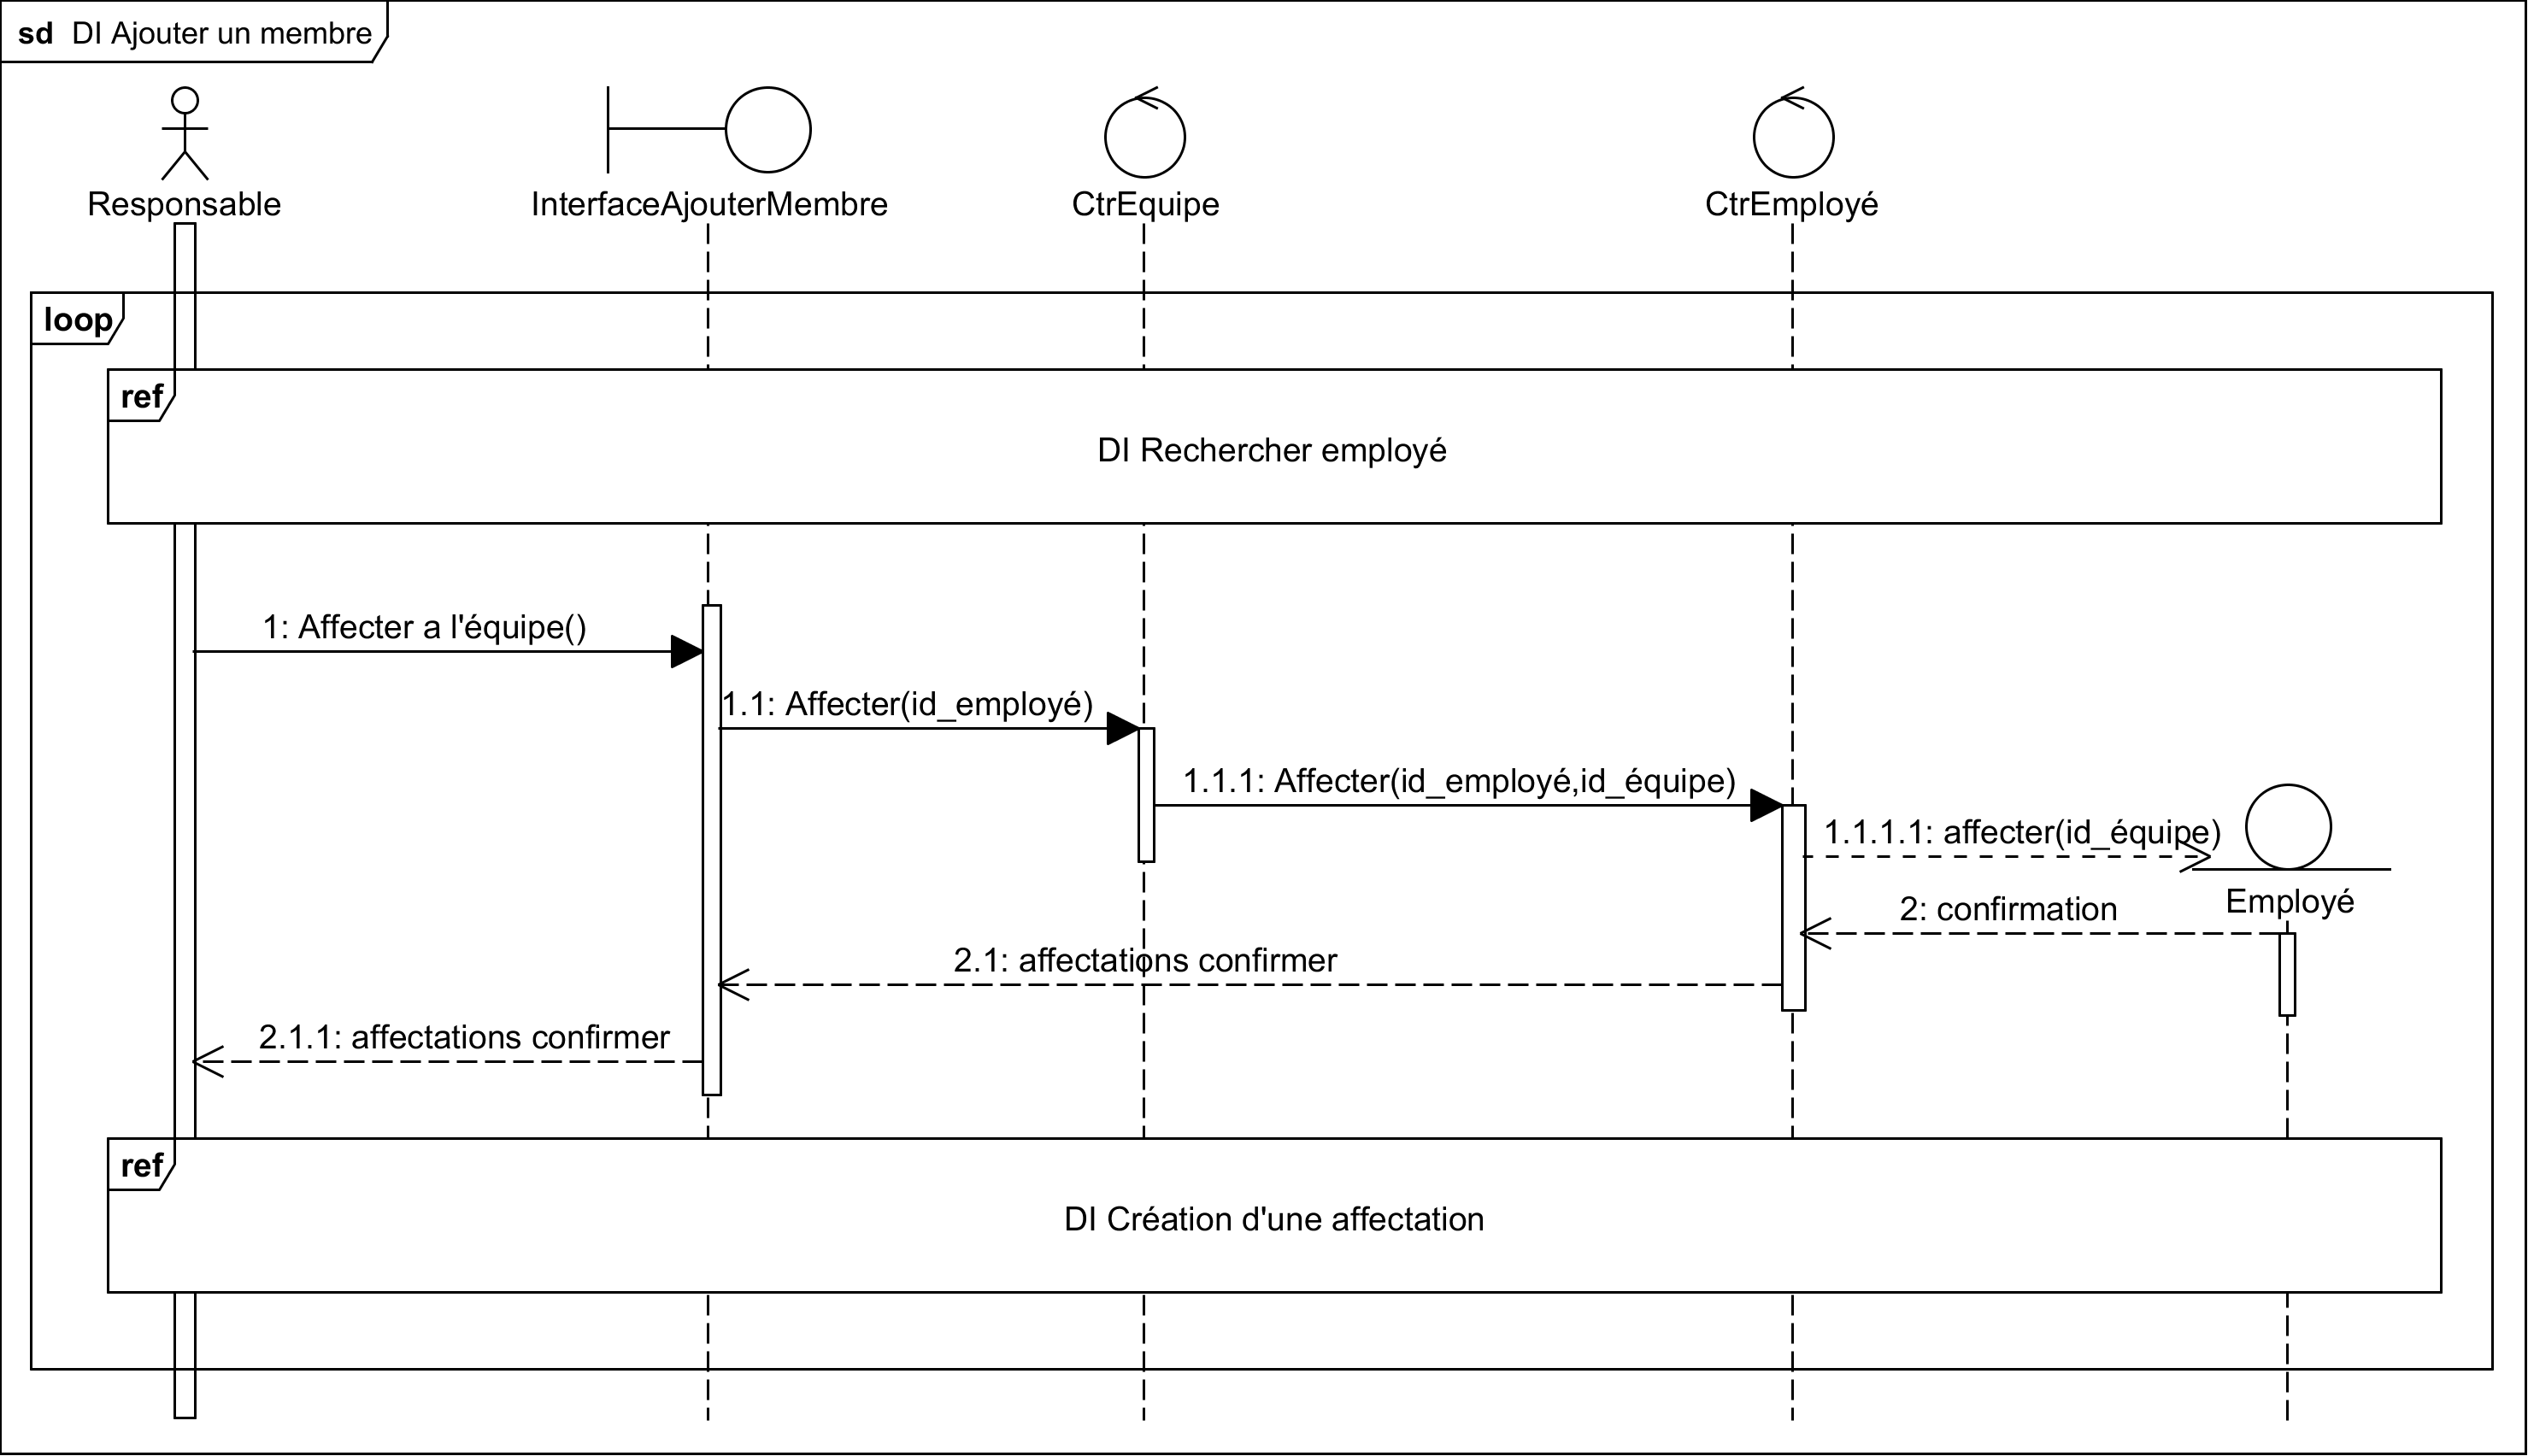
\includegraphics[ scale=0.69]{images/DS/DI Ajouter un membre.png}
    \caption{Diagramme d'interaction « Ajouter membre »}
    \label{fig40}
\end{figure}


\subsection*{Diagramme d'interaction du cas d'utilisation « Ajouter employé »}
À travers l’interface InterfaceGestionEmployé, l’administrateur aura la
possibilité d’ajouter un employé en saisissant les informations. Après la
validation, une vérification des données est effectuée avant l’ajout de
l’employé. Une fois créé, le contrôle ctrEmpreinte se chargera d’ajouter son
empreinte qui déclenchera la destruction de l’interface d’ajout et
l’administrateur sera redirigé vers l’interface InterfaceGestionEmployé avec la
nouvelle liste des employés.

\clearpage

\begin{figure}[h!]
    \centering
    \includegraphics[scale=0.7]{images/DS/DI Ajouter employé.png}
    \caption{Diagramme d'interaction « Ajouter employé »}
    \label{fig41}
\end{figure}

\subsection*{Diagramme d'interaction du cas d'utilisation « Consulter profil d'un employé »}
Une fois authentifié, le responsable aura la possibilité de consulter le profil
d’un employé. L’interface InterfaceProfileEmployé déléguera au contrôle
CtrEmployé la recherche de l’employé sélectionner, puis lui retournera les
informations concernant ce dernier. Il pourra aussi à travers cette interface
être redirigé vers l’interface de modification du profil ainsi que vers
l’interface qui lui permettra de consulter le planning de cet employé.
        
\clearpage
        
\begin{figure}[h!]
    \centering
    \includegraphics[scale=0.82]{images/DS/consulter_profil_d'un_employé.png}
    \caption{Diagramme d'interaction « Consulter profil d'un employé »}
    \label{fig42}
\end{figure}
    
\section{Diagramme de classes conception préliminaire}
En partant du modèle d’analyse, nous allons affiner et compléter les diagrammes 
de classes participantes obtenus précédemment. Pour cela, nous utiliserons les 
diagrammes de séquence que nous venons de réaliser pour:

\begin{itemize}
    \item [\textbullet] Ajouter ou préciser les opérations dans les classes 
        (un message ne peut être reçu par un objet que si sa classe a déclaré 
        l’opération publique correspondante).
    \item [\textbullet] Ajouter des types aux attributs et aux paramètres et 
        retours des opérations. 
    \item [\textbullet] Affiner les relations entre classes: associations 
        (avec indication de navigabilité), généralisations ou dépendances.\cite{5}
\end{itemize}
    
\clearpage

\subsection*{Diagramme de classes conception préliminaire du cas d'utilisation « Consulter ma fiche de pointage »}

\begin{figure}[h!]
    \centering
    \includegraphics[scale=0.74]{images/DCC/DCC Consulter ma fiche de pointage.png}
    \caption{Diagramme de classes conception préliminaire « Consulter ma fiche de pointage »}
    \label{fig42}
\end{figure}
        
\subsection*{Diagramme de classes conception préliminaire du cas d'utilisation « Ajouter une équipe »}

\clearpage

\begin{figure}[h!]
    \centering
    \includegraphics[scale=0.7]{images/DCC/DCC Ajouter une équipe.png}
    \caption{Diagramme de classes conception préliminaire « Ajouter une équipe »}
    \label{fig43}
\end{figure}
        
\subsection*{Diagramme de classes conception préliminaire du cas d'utilisation « Ajouter un planning »}

\begin{figure}[h!]
    \centering
    \includegraphics[scale=0.7]{images/DCC/DCC Ajoutert un planning.png}
    \caption{Diagramme de classes conception préliminaire « Ajouter un planning»}
    \label{fig44}
\end{figure}
        
\clearpage

\subsection*{Diagramme de classes conception préliminaire du cas d'utilisation « Ajouter un employé »}

\begin{figure}[h!]
    \centering
    \includegraphics[scale=0.7]{images/DCC/DCC Ajouter employé.png}
    \caption{Diagramme de classes conception préliminaire « Ajouter un employé»}
    \label{fig45}
\end{figure}

\subsection*{Diagramme de classes conception préliminaire du cas d'utilisation « Consulter profil d'un employé »}

\begin{figure}[h!]
    \centering
    \includegraphics[scale=0.74]{images/DCC/DCC Consulter profil d'un employé.png}
    \caption{Diagramme de classes conception préliminaire « Consulter profil d'un employé»}
    \label{fig46}
\end{figure}

\section{Diagramme de classe conception}
Les diagrammes de classes décrivent la structure ou plutôt l’architecture d’un
système et sont donc la base de presque toutes les autres techniques de
description. En conséquence, les diagrammes de classes, et en particulier les
classes, sont un concept qui est utilisé universellement en modélisation et en
programmation. Ils permettent l’encapsulation des attributs et des méthodes et
la représentation des instances sous forme d’objets\cite{10}.

À l’aide des diagrammes de classe de conception établis dans la section
précédente, nous avons modélisé le diagramme de classe ci-dessous.

\begin{figure}[h!]
    \centering
    \includegraphics[scale=0.69]{images/DCC/Diagramme de classe.png}
    \caption{Diagramme de classe}
    \label{fig47}
\end{figure}

\section{Modèle relationnel}
Le modèle relationnel a vu le jour en 1970 avec les travaux de Edgar Frank 
Codd. La principale publication est « A Relational Model for Large Shared Data 
Banks », Communications of the ACM, vol. 13, n° 6, 1970.\\

\begin{figure}[h!]
    \centering
    \includegraphics[scale=1]{images/pere_mr.PNG}
    \caption{Le père du modèle relationnel}
    \label{fig48}
\end{figure}
        
Ce modèle de données est construit principalement autour des concepts suivants \cite{11}:

\begin{itemize}
    \item[\textbullet] Relation: structure de données qui préfigure la table qui 
        sera créée à l’aide du langage SQL.
    \item[\textbullet]  Attribut: représentation d’une information atomique qui 
        préfigure une colonne d’une table. Un domaine de valeurs devrait être défini 
        ainsi que d’éventuelles règles de validation (contraintes).
    \item[\textbullet] Clé primaire: attribut(s) identifiant une relation qui 
        préfigure(nt) la primary Key de la table.
    \item[\textbullet] Clé étrangère: attribut(s) qui référence(nt) une tierce 
        relation, préfigure(nt) une foreign Key de la table.             
\end{itemize}

Afin de pouvoir implémenter une base de données, il faut pouvoir traduire le 
modèle conceptuel en modèle logique. Cela signifie qu’il faut pouvoir convertir 
un modèle UML en modèle relationnel. Les modèles conceptuels sont suffisamment 
formels pour que ce passage soit systématisé dans la plupart des cas. 
En appliquant les règles de passage\cite{12}, nous obtenons les relations suivantes:

\begin{itemize}
    \item [\textbullet]\textbf{Employé}(\underline{id\_employé}, nom, prénom, genre, 
        username, email,pwd, date\_naissance,lieu-naissance, adresse, présence, poste, 
        observations, tél\_professionnel, tél\_personnel, photo, \#ggid\_équipe, 
        \#ggid\_planning, \#id\_empreinte).

	\item [\textbullet]\textbf{Planning}(\underline{id\_planning}, intitulé, 
        description).
    
    \item [\textbullet]\textbf{Jour}(\underline{id\_jour}, h\_entrée1, h\_sortie1, 
        h\_entrée2, h\_sortie2, \#ggid\_planning).
    
    \item [\textbullet]\textbf{Équipe}(\underline{id\_équipe}, intitulé, 
        description, \#ggid\_manager).
    
    \item [\textbullet]\textbf{Affectation}(\underline{id\_affectation}, 
        rejoint\_jour, quitté\_jour, \#ggid\_équipe, \#id\_employé).
    
    \item [\textbullet]\textbf{Shift}(\underline{id\_shift},num\_séquence, 
        h\_entrée, h\_sortien, \#ggid\_employé ).
    
    \item [\textbullet]\textbf{Empreinte}(\underline{id\_empreinte}, 
        empreinte\_hash)
    
    \item [\textbullet]\textbf{Administrateur}(\underline{id\_administrateur}, 
        username, email, pwd).
\end{itemize}

\section{Conclusion}
Au cours de ce chapitre, nous avons en premier lieu identifié les modèles du
domaine pour avoir une vue globale sur les différentes entités de notre système,
puis nous avons modélisé les diagrammes de classes participantes et
d’interactions qui permettent l’enrichissement des diagrammes de séquences
système. Par la suite, en modélisant les diagrammes de classe conception
préliminaire, nous avons pu établir le diagramme de classe conception.  Enfin,
pour avoir une vue plus structurée et implémenter une base de données nous avons
traduit ce dernier diagramme en un modèle relationnel. 


%%%% Chapitre 4 %%%%
\chapter{Réalisations de la pointeuse}
\fancyhead[R]{\textit{Réalisations et programmation de la pointeuse}}
\renewcommand{\headrulewidth}{1pt}

\section{Introduction}
Dans ce chapitre, nous aborderons l’aspect matériel du projet en l’occurrence la pointeuse biométrique à réaliser. En premier lieu, nous allons décrire Arduino en tant que plateforme, puis nous décrirons en détail le microcontrôleur choisi en justifiant le choix de ce dernier. Par la suite, nous citerons les caractéristiques du capteur d’empreinte. Une fois assemblés, ils formeront notre dispositif de pointage. Nous exposerons les différents schémas de branchement et réaliserons un prototype en 3D pour avoir un aperçu de l’objet à concevoir. 
La dernière section de ce chapitre concerne la communication entre la pointeuse et le système de gestions de pointage.

\section{Arduino}
Arduino est la marque d’une plateforme de prototypage open source, elle permet aux utilisateurs de créer des objets électroniques interactifs à partir de cartes électroniques matériellement libres sur lesquelles se trouve un microcontrôleur (d’architecture Atmel AVR. comme l’Atmega328p, et d’architecture ARM comme le Cortex-M3 pour l’Arduino due).

Les schémas de ces cartes électroniques sont publiés en licence libre. Cependant, certaines composantes, comme le microcontrôleur par exemple, ne sont pas sous licence libre. Le microcontrôleur peut être programmé pour analyser et produire des signaux électriques, de manière à effectuer des tâches très diverses comme la domotique (le contrôle des appareils domestiques — éclairage, chauffage…), le pilotage d’un robot, de l’informatique embarquée, etc. Arduino peut être utilisé pour construire des objets interactifs indépendants (prototypage rapide), ou bien peut être connecté à un ordinateur pour communiquer avec ses logiciels (ex. : Max/MSP, Usine Hollyhock, pure Data, SuperCollider).

    \subsection{Matériel}
    Un module Arduino est généralement construit autour d’un microcontrôleur Atmel AVR. (ATmega328, ATmega32u4 ou ATmega2560 pour les versions récentes, ATmega168, ATmega1280 ou ATmega8 pour les plus anciennes), et de composants complémentaires qui facilitent la programmation et l’interfaçage avec d’autres circuits. Le microcontrôleur est préprogrammé avec un Bootloader, de telle sorte qu’un programmateur dédié ne soit pas nécessaire. Les modules sont programmés avec une connexion série TTL, mais les connexions permettant cette programmation diffèrent selon les modèles. Les premiers Arduino possédaient un port série RS-232, puis l’USB est apparu sur les modèles Diecimila, tandis que certains modules destinés à une utilisation portable comme le Lillypad ou le promini se sont affranchis de l’interface de programmation, relocalisée sur un module USB-série dédié (sous forme de carte ou de câble). Les modules d’extension venant s’empiler sur l’Arduino. Plusieurs sortes d’extensions sont disponibles dans le commerce.
    Plusieurs cartes compatibles Arduino ont été produites par d’autres fabricants. Il existe aussi des cartes Arduino ou compatibles modifiés pour un usage spécifique : par exemple, des cartes de contrôle pour imprimantes 3D RepRap20, des systèmes de pilote automatique pour drones comme les systèmes ArduPilot, APM : Plane et APM:Copter, ou les cartes FlyDuino21, enfin des puces Wi-Fi tierces comme l’ESP8266 compatible avec l’environnement Arduino22.\cite{30}

    \subsection{Logiciel}
    Le logiciel de programmation des modules Arduino dont l’interface est appelée Arduino IDE, est une application Java, libre et multiplateforme dérivée de Processing servant d’éditeur de code et de compilateur, et qui peut transférer le firmware et le programme au travers de la liaison série (RS-232, Bluetooth ou USB selon le module). Il est également possible de se passer de l’interface Arduino, et de compiler et téléverser les programmes via l’interface en ligne de commande. Le langage de programmation utilisé est le C++, compilé avec avr.-g++ 8, et lié à la bibliothèque de développement Arduino, permettant d’utiliser la carte et ses entrées/sorties. La mise en place de ce langage standard rend aisé le développement de programmes sur les plateformes Arduino à toute personne maîtrisant le C ou le C++.\cite{31}


\section{ESP32}
    ESP32 est une série de microcontrôleurs de type système sur une puce (SoC) d’Espressif Systems, basé sur l’architecture Xtensa LX6 de Tensilica (en), intégrant la gestion du Wi-Fi et du Bluetooth (jusqu’à LE 5.0 et 5.11) en mode double, et un DSP. C’est une évolution d’ESP8266.Son support Wi-Fi et Bluetooth, en fait un système apprécié dans le domaine de l’internet des objets. Ce SoC rencontre un certain succès depuis quelques années à la fois pour son coût, ses capacités et son intégration dans un nombre croissant de systèmes.\cite{32}
    \begin{figure}[h!]
                 \centering
                \includegraphics[scale=0.30]{images/esp32.jpg}
                 \caption{ESP32 DevKit}
                 \label{fig49}
    \end{figure}
    \subsection{Caractéristiques techniques}\cite{33}
        \begin{itemize}
            \item[\textbullet]\textbf{Processeurs :}
                \begin{itemize}
                    \item CPU : Xtensa double-cœur (ou simple-cœur), microprocesseur LX 32 bits, fonctionnant à 160 ou 240 MHz et fournissant jusqu'à 600 DMIPS ;
                    \item coprocesseur ultra basse consommation (ULP) ;
                \end{itemize}
            \item[\textbullet]\textbf{Mémoire :} 520 KiO SRAM ;
            \item[\textbullet]\textbf{Connectivité sans-fil :}
                \begin{itemize}
                    \item Wi-Fi : 802.11 b/g/n ;
                    \item Bluetooth : v 4.2 BR/EDR et BLE jusqu'à v 5.0 et v 5.1 ;
                \end{itemize}
            \item[\textbullet]\textbf{Interfaces de périphériques}
                 \begin{itemize}
                    \item 12-bit Segmentation sur les ADC (SAR ADC) jusqu'à 18 canaux ;
                    \item 2 × 8 bit DAC ;
                    \item 10 × capteurs de touché (GPIO de capteur capacitif (en)) ;
                    \item 4 × SPI ;
                    \item 2 × interfacs I²S ;
                    \item 2 × interfaces I²C ;
                    \item 3 × UART ;
                    \item contrôleur hôte SD/SDIO/CE-ATA (en)/MMC/eMMC ;
                    \item contrôleur esclave SDIO/SPI ;
                    \item interface MAC Ethernet avec DMA dédié et support du protocole de temps précis IEEE 1588 ;
                    \item Bus de données CAN 2.0 ;
                    \item contrôleur infrarouge distant (TX/RX, jusqu'à 8 canaux) ;
                    \item Moteur PWM ;
                    \item LED PWM (jusqu'à 16 canaux) ;
                    \item Capteur à effet Hall ;
                    \item préamplificateur analogique ultra-basse consommation ;
                \end{itemize}
            \item[\textbullet]\textbf{Sécurité}
                \begin{itemize}
                    \item Standard de sécurité supportant complètement IEEE 802.11,incluant WPA/WPA2 et WAPI de WFA ;
                    \item Secure boot (démarrage sécurisé) ;
                    \item Chiffrement de la Flash ;
                    \item 1024-bit OTP, jusqu'à 768 bits pour les clients
                    \item Accélération matérielle du chiffrement : AES, SHA-2, RSA, elliptic curve cryptography (ECC), générateur de nombre aléatoire (en) (RNG) ;
                \end{itemize}
            \item[\textbullet]\textbf{Gestion de l'énergie}
                \begin{itemize}
                    \item low-dropout regulator (en) interne;
                    \item Domaines d'alimentation individuels pour le RTC;
                    \item Alimentation en sommeil profond de 5 μA ;
                    \item Réveil depuis des interruptions GPIO, timer, mesure ADC, interruption du capteur de touché capacitif.
                \end{itemize}
        \end{itemize}
     
    
    \begin{figure}[h!]
                 \centering
                    \includegraphics[scale=0.26 ]{images/esp32_fun.png}
                 \caption{Schéma fonctionnel}
                 \label{fig50}
    \end{figure}
   Le choix du module ESP32 Devkit est justifié par sa petite taille (57mm*28mm*3m), ainsi que ses caractéristiques notamment les connectivités sans-fil, Sécurité et gestion de l’énergie.

        
\section{Capteur d'empreinte DY 50}
Les techniques utilisées pour capter les images des empreintes digitales sont diverses, d’où l’existence de plusieurs types de capteurs on peut citer :
    \begin{itemize}
        \item le capteur thermique.
        \item le capteur en silicium.
        \item le capteur ultrasonique.
        \item le capteur capacitif.
        \item le capteur à champ électrique.
        \item le capteur à pression.
        \item le capteur optique.
    \end{itemize}
    Pour les besoins de notre projet nous avons choisi le capteur DY50 de type optique en raison de son coût, sa taille et du fait d’avoir une image précise de l’empreinte tout en étant intrinsèquement protégé contre les décharges électrostatiques.
    \begin{figure}[h!]
                 \centering
                    \includegraphics[scale=0.8]{images/dy50.jpg}
                 \caption{Capteur optique DY50}
                 \label{fig51}
    \end{figure}
    \subsection{Principe de fonctionnement}
    Grâce au principe de l’imagerie optique, les lignes créées par l’irrégularité de la peau sur la face interne du doigt formeront diverses images d’empreintes digitales. La texture de la peau est différente par les motifs, les points de rupture et les intersections. Ils sont appelés dans le traitement de l’information « Points caractéristiques », les caractéristiques de chaque doigt sont différentes, c’est-à-dire uniques, en s’appuyant sur cette unicité, nous pouvons associer une personne à son empreinte digitale, en préstockant son empreinte digitale.
    
    Le système d’identification d’empreintes digitales collecte, analyse et compare les empreintes digitales grâce à un équipement de conversion photoélectrique spécial et à une technologie de traitement d’image, et peut identifier automatiquement, rapidement et avec précision l’identité personnelle. Le système comprend principalement des processus tels que l’acquisition d’images d’empreintes digitales, le traitement d’images d’empreintes digitales, l’extraction de caractéristiques, ainsi que la comparaison et la correspondance des valeurs des caractéristiques.\cite{34}
    \begin{longtable}{|p{1.3cm}|p{1.8cm}|p{1.8cm}|p{10cm}|}
                % header and footer information
                \endhead
                \endfoot
                % body of table
                \hline
                Broche & Nom & Type & Description fonctionnelle \\
                \hline
                1 & GND & Dans & Module d'alimentation l'apport positif \\
                \hline
                2 & TXD & Sur & Sortie de données série TTL. Niveau logique TTL \\
                \hline
                3 & RXD & Dans & Entrée de données série TTL. Niveau logique TTL \\
                \hline
                4 & 3.3V & - & Masse du Signal. Connexion à la terre interne et électrique 
                \\
                \hline
                5 & Tactile & Sur & Sortie de signal d'induction, niveau élevé par défaut efficace 
                \\
                \hline
                6 & TouchVin & Dans & Entrée d'alimentation à détection tactile, alimentation 3.3v 
                \\
                \hline
                \caption{Interface de connexion}\cite{34}\\
        \end{longtable}   

     \subsection{Caractéristiques techniques }
     \begin{itemize}
        \item Tension d'alimentation: cc 3.6 ~ 6.0V / 3.3V fournissant.
        \item Courant d'alimentation: courant: <120mA.
        \item Courant de crête: <140mA.
        \item Temps d'image d'empreinte digitale: <1.0 seconde.
        \item Taille de fenêtre: 14*18mm.
        \item Mode correspondant: mode Match (1:1).
        \item Mode de recherche (1: N).
        \item Fichier de Signature: 256 octets.
        \item Fichiers de modèle: 512 octets.
        \item Capacité de stockage: 127.
        \item Niveau de sécurité: cinq (de bas à haut: 1,2,3,4,5).
        \item Faux taux d'acceptation (FAR): <0.001\% (niveau de sécurité 3).
        \item Taux de faux rejet (FRR): <1.0\% (niveau de sécurité 3).
        \item Temps de recherche: <1.0 seconde (1:500, la moyenne).
        \item Interface PC: UART (niveau logique TTL) ou USB2.0 / USB1.1.
        \item Débit en bauds de Communication (UART): (9600 * N) bps où N = 1 ~ 12 (valeur par défaut N =6, soit 57600bps).
        \item Environnement de travail:
        \begin{itemize}
            \item [\textbullet]Température: -20 ° - + 50.
            \item [\textbullet]Humidité Relative: 40\% RH-85 \% hr (sans condensation).
        \end{itemize}
        
        \item Environnement de stockage:
        \begin{itemize}
            \item [\textbullet] Température: -40 - + 85².
            \item [\textbullet] Humidité Relative: <85\% H (sans condensation).
        \end{itemize}
        \
        \item Dimensions (L * W * H): 56*20*21.5mm .
     \end{itemize}
     

\section{Schémas et branchement}

    \begin{figure}[h!]
                    \centering
                    \includegraphics[scale=0.2]{images/schema/montage_illustration.png}
                    \caption{Schéma expliquant le montage préliminaire des différents modules  }
                    \label{fig52}
    \end{figure}
     Le schéma ci-dessus révèle la manière dont le module ESP32 Devkit ainsi que le capteur d’empreinte DY50 on était connecté, ainsi qu’une LED pour signaler a l’utilisateur la réussite ou l’échec des différentes opérations.\clearpage  
    Branchement: 
    \begin{itemize}
        \item [\textbullet]TX (ESP32) -> RX (DY50)
        \item [\textbullet]RX (ESP32) -> TX (DY50)
        \item [\textbullet]GND (ESP32) -> GND (DY50) 
        \item [\textbullet]3.3v (ESP32) -> vcc (DY50)
        
    \end{itemize}            
                
               
                
    Afin d’améliorer l’expérience utilisateur nous avons rajouté un écran qui permettra d’afficher les différents messages comme la réussite ou l’échec du pointage ou le nombre d’empreintes enregistrer.
                \begin{figure}[h!]
                    \centering
                    \includegraphics[scale=0.2]{images/schema/schemat v3 sans uvc.png}
                    \caption{Schéma expliquant le montage préliminaire des différents modules  }
                    \label{fig53}
                \end{figure}
    
    Branchement: 
    \begin{itemize}
        \item [\textbullet]GPIO21 (ESP32) -> SLC (OLED Display)
        \item [\textbullet]GPIO22 (ESP32) -> SDA (OLED Display)
        \item [\textbullet]GND (ESP32) -> GND (OLED Display) 
        \item [\textbullet]3.3v (ESP32) -> VCC (OLED Display)
    \end{itemize}    
    
    
                \begin{figure}[h!]
                    \centering
                    \includegraphics[scale=0.2]{images/schema/schemat_globale.png}
                    \caption{Schéma expliquant le montage préliminaire des différents modules  }
                    \label{fig54}
                \end{figure}
      Compte tenu du contexte actuel (crise sanitaire due au virus COVID-19) et afin de limiter la propagation du virus des gestes barrières sont recommandé. Par ailleurs, le fait de toucher une surface ayant était en contact avec plusieurs individus sans que cette dernière soit désinfecter au préalable constitue un risque sanitaire. Pour remédier à ce problème, nous avons décidé d’équiper notre pointeuse d’une LED UV-C (lampe germicide). Néanmoins, ce composant doit faire l’objet d’une recherche plus approfondie pour confirmer la possibilité de l’installer, car la longueur d’onde de ce type de lumière peut avoir des effets secondaires indésirables en cas de fortes expositions.

    Pour garantir la disponibilité et l’accessibilité du service de pointage, la pointeuse doit être fonctionnelle même en cas d’absence de courant. Afin de remédier à cette contrainte, nous avons décidé d’inclure une source d’alimentation secondaire (batterie) qui alimentera tout le dispositif de pointage en cas de coupure de courant à supposer que le serveur hébergeant le système dispose lui aussi d’une alimentation d’urgence en cas de coupure.    
   
   
\section{Prototype}
Le prototype matérialise une étape d’évolution d’un projet, souvent pour démontrer ou infirmer le bien-fondé d’un ou plusieurs concepts mis en jeu dans ce projet, avant toute valorisation commerciale.
Nous avons décidé de réaliser un prototype en 3D du dispositif de pointage afin d’avoir une idée du résultat final.
\clearpage
    \begin{figure}[!htb]
       \begin{minipage}{0.5\textwidth}
         \centering
         \includegraphics[scale=0.6]{images/prototype/1.png}
         \caption{Pointeuse vue de face}\label{ }
       \end{minipage}\hfill
       \begin{minipage}{0.5\textwidth}
         \centering
         \includegraphics[scale=0.6]{images/prototype/2.png}
         \caption{Pointeuse vue de haut}\label{ }
       \end{minipage}
    \end{figure}
    
    \begin{figure}[!htb]
       \begin{minipage}{0.5\textwidth}
         \centering
         \includegraphics[scale=0.16]{images/prototype/5.png}
          \vspace{-20pt}
         \caption{Côté gauche extérieure}\label{ }
       \end{minipage}\hfill
       \begin{minipage}{0.5\textwidth}
         \centering
         \includegraphics[scale=0.16]{images/prototype/6.png}
          \vspace{-20pt}
         \caption{Côté gauche intérieure}\label{ }
       \end{minipage}
    \end{figure}
    \clearpage    

    \begin{figure}[!htb]
        \vspace{-40pt}
       \begin{minipage}{0.5\textwidth}
         \centering
         \includegraphics[scale=0.16]{images/prototype/3.png}
          \vspace{-40pt}
         \caption{Pointeuse ouverte}\label{ }
       \end{minipage}\hfill
       \begin{minipage}{0.5\textwidth}
         \centering
         \includegraphics[scale=0.16]{images/prototype/4.png}
         \vspace{-40pt}
         \caption{Pointeuse fermer}\label{ }
       \end{minipage}
    \end{figure}


    Les images précédentes représentent la disposition des différents composants dans un boîtier. Elles nous donnent un aperçu sur l’aspect extérieur de la pointeuse et de sa forme. Il est utile de préciser que le lecteur dispose d’un cache rétractable une manœuvre obligatoire lorsque :
    \begin{itemize}
        \item [\textbullet] la LED UV-C est utilisée pour désinfecter la surface de lecture d’empreinte du capteur. Afin de protéger les utilisateurs des effets indésirables des rayonnements ultraviolets.
        \item [\textbullet]  Le dispositif est transporté ou déplacé afin de protéger la surface en verre de toute dégradation ou égratignure qui peuvent affecter les performances de la pointeuse ou la rendre complètement défectueuse.  
    \end{itemize}
    
    
\section{Programmation}
Une fois les parties matérielles correctement assemblées, nous allons passer à la partie programmations de la pointeuse. En premier lieu, nous allons définir le rôle de chaque composant ainsi que son champ d’action.
\begin{itemize}

    \item[\textbullet] \textbf{Le module ESP32 DevKit:} Ce dernier représente le cerveau de la pointeuse. Car le programme de la pointeuse sera logé en lui. Il sera responsable de la communication entre la pointeuse et l’application. Il exécutera les différentes commandes exigées par l’administrateur (changement de mode enregistrement/suppression/pointage, suppression de la base de donnés des empreintes au niveau du capteur d’empreinte).  
    
    \item[\textbullet] \textbf{Le capteur d'empreinte DY50:} Ce dernier représente un périphérique d’entrée d’empreinte à l’aide de sa mémoire interne, on pourra sauvegarder les images détaillées des empreintes, ce qui minimise drastiquement le temps de reconnaissance des différentes empreintes vu que leurs images sont déjà présentes dans la mémoire du capteur.
        
    Comme expliqué précédemment la plateforme Arduino permet de travailler avec des modules compatibles, mais s’ils sont issus d’un autre fabricant. Ce qui est le cas concernant le module ESP32 Devkit et notre capteur d’empreintes DY50. Néanmoins il est indispensable de télécharger les pilotes et les librairies des fabricants.    
\end{itemize}
    \subsection{Environnement de travail}
        
            \subsubsection{Arduino IDE }
                Le logiciel de programmation des cartes Arduino est une application Java, libre et multiplateforme, servant d'éditeur de code et de compilateur qui peut transférer le programme au travers de la liaison série (RS-232, Bluetooth ou USB selon le module). Il est également possible de se passer de l'interface Arduino, et de compiler les programmes via l'interface en ligne de commande.
                
                \begin{figure}[h!]
                    \centering
                    \includegraphics[scale=0.3]{images/arduino_ide.PNG}
                    \caption{interface Arduino IDE et un programme qui clignote une LED}
                    \label{fig61}
                \end{figure}
                
                
             \subsubsection{Langage de programmation C}
                le C est un langage de programmation impératif généraliste de bas niveau. Inventé au début des années 1970 pour réécrire UNIX, c’est devenu un des langages les plus utilisés, encore de nos jours. De nombreux langages plus modernes comme C++, C#, Java et PHP ou JavaScript ont repris une syntaxe similaire et reprennent en partie sa logique. Il offre aux développeurs une marge de contrôle importante sur la machine (notamment sur la gestion de la mémoire) et est de ce fait utilisé pour réaliser les « fondations » (compilateurs, interpréteurs…) de ces langages plus modernes.

                Ces caractéristiques en font un langage privilégié quand on cherche à maîtriser les ressources matérielles utilisées, le langage machine et les données binaires générées par les compilateurs étant relativement prévisibles. Ce langage est donc extrêmement utilisé dans des domaines comme la programmation embarquée sur microcontrôleurs, les calculs intensifs, l’écriture de systèmes d’exploitation et les modules où la rapidité de traitement est importante. Il constitue une bonne alternative au langage d’assemblage dans ces domaines, avec les avantages d’une syntaxe plus expressive et de la portabilité du code source. Le langage C a été inventé pour écrire le système d’exploitation UNIX, et reste utilisé pour la programmation système. Ainsi le noyau de grands systèmes d’exploitation comme Windows et Linux sont développés en grande partie en C.
                
                En contrepartie, la mise au point de programmes en C, surtout s’ils utilisent des structures de données complexes, est plus difficile qu’avec des langages de plus haut niveau. En effet, dans un souci de performance, le langage C impose à l’utilisateur de programmer certains traitements (libération de la mémoire, vérification de la validité des indices sur les tableaux…) qui sont pris en charge automatiquement dans les langages de haut niveau\cite{35}.
                
                
             \subsubsection{esspresif/arduino-esp32 library}
             Une librairie écrite et maintenue par le constructeur ESSPRISIF. Cette dernière doit être installée au niveau de l'IDE Arduino pour pouvoir téléverser les programmes écrits sur le module ESP32 Devkit. Elle est disponible sur : <https://github.com/espressif/arduino-esp32>
             \subsubsection{Adafruit fingerprint sensor library}
              Pour pouvoir interagir avec le capteur d'empreinte cette librairie est nécessaire, car elle implémente les différentes méthodes et fonctions qui régissent le fonctionnement de capteur d'empreinte DY50 on peut citer :
              \begin{itemize}
                  \item[\textbullet] check\_model(): qui vérifie le statut du capteur d'empreinte. Retourne l'erreur ou OK.
                  \item[\textbullet] count\_template(): qui demande au capteur de compter le nombre d'empreintes dans ça mémoire et stocker cette valeur dans \emph{self.template\_count}.
                  \item[\textbullet] creat\_model(): qui demande au capteur de transformer l'empreinte en un modèle exploitable.Renvoi le code d'erreur du packet ou OK.
                  \item[\textbullet] delet\_model(localisation): qui demande au capteur de supprimer un modèle d'empreinte de la mémoire flash apres l'avoir sélectionné grâce à l'argument 'localisation'.Retourne l'erreur ou OK.
                  
                  \item[\textbullet] empety\_librery() : qui demande au capteur de réinitialiser toute la mémoire flash ainsi supprimer tous les modelés précédemment enregistrer. 
                  \item[\textbullet] get\_image() : qui demande au capteur de capturer une image et de l'enregistrer dans la mémoire.Retourne l'erreur ou OK. 
                  \item[\textbullet] finger\_search() : qui demande au capteur de chercher l'empreinte correspondante à partir de slot 1,enregistre la localisation et le taux de correspondance dans \emph{in self.finger\_id} et \emph{self.confidence}.Renvois l'erreur ou Ok.\cite{36}
              \end{itemize}
              
    \subsection{Code et fonctionnement}    
    comme la plupart des programmes destinés ont des modules ou compatibles Arduino le programme à téléverser est constitué de : 
    
    \begin{itemize}
        \item [\textbullet] une partie pour déclarations des librairies utilisées et des variables globales
    \end{itemize}
    \begin{minted}{c}
            #include <Adafruit_Fingerprint.h>
            #include <HardwareSerial.h>
            #include <WiFi.h>
            #include <HTTPClient.h>

            const char *ssid = "TP-LINK_9C42F4";
            const char *password = "********";
            // post array that will be send to the website
            String postData;    
            //computer IP or the server domain 
            String linkee = "http://192.168.1.222:8000/pointage/getid"; 
            // The Fingerprint ID from the scanner
            uint8_t id; 

            Adafruit_Fingerprint finger = Adafruit_Fingerprint(&Serial2);
            int FingerID = 0;

        \end{minted}
    le code précédent représente la partie déclarative de notre programme ou nous avons inclus les librairies nécessaires (<Adafruit\_Fingerprint.h>, <HardwareSerial.h>, <WiFi.h>, <HTTPClient.h>) au fonctionnement de la pointeuse ainsi que les variables globales utilisées (postData, postData, linkee, id).
        
    \begin{itemize}
        \item [\textbullet] une partie void setup(): qui ne s’exécute qu’une seule fois est la partie où nous initialisons et configurons nos entrées/sorties et variables 
    \end{itemize}    
    \begin{minted}{c}
        void setup(){
            pinMode(2, OUTPUT);
            Serial.begin(115200);
            connectToWiFi();

        // set the data rate for the sensor serial port
            finger.begin(57600);
            Serial.println("\n\nAdafruit finger detect test");
            
            //------------*test the connection*------------
            if (finger.verifyPassword()){
              Serial.println("Found fingerprint sensor!");
            }else{
              Serial.println("Did not find fingerprint sensor :(");
              while (1)
              {
                delay(1);
              }
            }
            //---------------------------------------------
            finger.getTemplateCount();
            Serial.print("Sensor contains ");
            Serial.print(finger.templateCount);
            Serial.println(" templates");
            
 
            
            //SendFingerprintID( FingerID );
            //-------------* deleting all templates"-----------
            //emptyDataBase();
        
            }
    \end{minted}
   Dans cette section du code, nous avons initialisé la fréquence de transmission des différents modules. Ouvrir une connexion au point d’accès déclarer précédemment. Tester la liaison entre l’ESP32 et le capteur. Afficher le nombre d’empreintes enregistrer dans le capteur (lors de la phase de test).      
        
    \begin{itemize}
        \item [\textbullet] une partie void loop(): est la partie principale où se déroule le programme. Tout ce qui va être écrit dans cette zone sera exécuté par la carte en boucle. 
    \end{itemize}
    \begin{minted}{c}
        void loop(){
            //check if there's a connection to WiFi or not
              if (WiFi.status() != WL_CONNECTED){
                connectToWiFi();
              }
              //The ID start form 1 to 127
              // Get the Fingerprint ID from the Scanner
              FingerID = getFingerprintID(); 
              //don't need to run this at full speed.
              Serial.println(FingerID);
              delay(50);
              checkfinger();
              if (FingerID == 1){
                Serial.println("mode Enregistrement/Suppression ");
                checkToDelete();
                delay(5000);
                checkToAdd();
              }
            }
    \end{minted}
   Cette partie qui sera exécutée en boucle, elle englobe le comportement que va adopter la pointeuse une fois en service. Une fois la connexion au point d’accès établie et le capteur correctement connecté. 
    
    \begin{itemize}
        \item[\textbullet] une partie pour les différentes procédures et méthodes utiliser 
    \end{itemize}
    \begin{minted}{c}
            void checkToAdd(){
                HTTPClient http; //Declare object of class HTTPClient
                //Post Data
                // Add the Fingerprint ID to the Post array in order to send it 
                postData = "Get_Fingerid=get_id"; 
                // Post methode
                //initiate HTTP  request, put your Website URL or Your Computer IP
                http.begin(linkee);                                              
                //Specify content-type header
                http.addHeader("Content-Type", "application/x-www-form-urlencoded"); 
        
                int httpCode = http.POST(postData); //Send the request
                String payload = http.getString();  //Get the response payload
        
                if (payload.substring(0, 6) == "add-id"){
                    // Serial.println("j’ai reçu une réponse qui contient add id");
                    String add_id = payload.substring(6);
                    Serial.println(add_id);
                    id = add_id.toInt();
                    if (id != 0){
                        Serial.println("posez votre empreinte ");
                        getFingerprintEnroll();
                        }
                    }
                //Close connection
                http.end(); 
            }
    \end{minted}
    Cette partie du code représente une des nombreuses fonctions déclarées au niveau de la quatrième partie de notre programme. La méthode checkToAdd() a pour rôle de vérifier si une empreinte est en attente d’enregistrement après avoir consulté la base de données du système. Dans le cas d’une réponse « add-idN°empreinte » le capteur enclenche le processus d’enregistrement d’une nouvelle empreinte.

    Il existe plusieurs fonctions dans le programme destiner a la pointeuse (sendFingerPrintID, confirmAdding, checkFinger, etc.) nous avons décider de présenter celle-ci à titre d’exemple.
    
\section{Conclusion}
Dans ce chapitre, nous avons présenté les différentes phases de la réalisation de la pointeuse ainsi que les différents composants la constituant et les outils utilisés. Après avoir brièvement présenté la plateforme Arduino, nous avons exposé les caractéristiques du module ESP32 Devkit ainsi que du capteur d’empreinte DY50. Puis nous avons illustré le branchement des différentes parties. À l’aide au prototype, on a modélisé en 3D la pointeuse.
Maintenant qu’on peut concrètement identifier chaque individu grâce à son empreinte, on peut passer à l’étape suivante qui est la réalisation du système responsable d’exploiter cette information.  



%%%% Chapitre 5 %%%%
\chapter{implémentations mise en service et test}
\fancyhead[R]{\textit{implémentations mise en service et test}}
\renewcommand{\headrulewidth}{1pt}


\section{Introduction}
Ce chapitre sera consacré à la présentation de l’environnent de développement et des librairies utilisées. Ensuite, nous expliquerons l’architecture globale du système ainsi que son principe de fonctionnement. La deuxième partie sera réservée à la présentation de l’application dans ses différents aspects en commençant par sa charte graphique et la hiérarchie des pages de l’application web. Enfin, nous illustrerons quelques interfaces issues de l’application et nous aborderons brièvement le côté sécurité de l’application réalisée.   

\section{Environnement de développement}
Un environnement de développement se réfère à une suite d’applications et d’outils qui permettent un développement d’application facile. Par exemple, gérez des fichiers sources, déboguez du code, et enfin testez l’application avant de la lancer sur un environnement de test ou de production, dans cette section nous allons présenter l’environnement de développement utilisé pour développer notre application web.
    
    \subsection{Plateformes utilisés}
        \subsubsection*{Slack}
            \begin{wrapfigure}{r}{0.09\textwidth}
                \vspace{-22pt}
              \begin{center}
                 \includegraphics[scale=0.36]{images/logo/slack.png}
                 \label{fig62}
              \end{center}
              \vspace{-20pt}
              \vspace{-10pt}
            \end{wrapfigure}
            Slack est une  plateforme de communication collaborative propriétaire, elle permet de facilité l’organisation grâce à un système de canaux centralisant tout ce qui concerne un projet, un sujet ou une équipe, elle permet également de conservez les fichiers et les messages partager dans ces canaux\cite{37}. 

        \clearpage
        
        \subsubsection*{Trello}
        
            \begin{wrapfigure}{r}{0.09\textwidth}
                \vspace{-22pt}
              \begin{center}
                 \includegraphics[scale=0.36]{images/logo/trello.png}
                 \label{fig63}
              \end{center}
              \vspace{-20pt}
              \vspace{-10pt}
            \end{wrapfigure}
            Trello est un outil de gestion de projet en ligne, lancé en septembre 2011. Il repose sur une organisation des projets en planches listant des cartes, chacune représentant des tâches. Les cartes sont assignables à des utilisateurs et sont mobiles d’une planche à l’autre, traduisant leur avancement. Il permet donc d’organiser les projets et de définir leur ordre de priorité de façon amusante, souple et enrichissante\cite{38}.
        \subsubsection*{Github}
            \begin{wrapfigure}{r}{0.09\textwidth}
                \vspace{-22pt}
              \begin{center}
                 \includegraphics[scale=0.36]{images/logo/github.png}
                 \label{fig64}
              \end{center}
              \vspace{-20pt}
              \vspace{-10pt}
            \end{wrapfigure}
            GitHub est une plateforme de développement qui offre un service d’hébergement qui permet aux développeurs de stocker et de partager, publiquement ou non, le code qu’ils créent, il fournit aussi plusieurs fonctionnalités de collaboration, telles que des wikis et des outils de gestion des tâches de base pour chaque projet\cite{40}.
        
        \subsubsection*{Discord}
        
            \begin{wrapfigure}{r}{0.09\textwidth}
                \vspace{-22pt}
              \begin{center}
                 \includegraphics[scale=0.36]{images/logo/discord.png}
                 \label{fig65}
              \end{center}
              \vspace{-20pt}
              \vspace{-10pt}
            \end{wrapfigure}
            Discord est une plateforme gratuite qui offre un service de communication par chat vidéo, vocal et textuel, il est donc utile et nécessaire de l’utiliser pour une communication en continu surtout en temps de pandémie\cite{40}.
        
    
    \subsection{Logiciels utilisés}
    
        \subsubsection*{Visual studio code}
            \begin{wrapfigure}{r}{0.09\textwidth}
              \vspace{-20pt}
              \begin{center}
                \includegraphics[width=0.09\textwidth]{images/VSCode logo.png}
                \label{fig66}
              \end{center}
              \vspace{-20pt}
              \vspace{-10pt}
            \end{wrapfigure}
            Visual Studio Code (VSCode) est un éditeur de code source, développé par Microsoft en tant que projet open source, il s’agit de l’outil d’environnement de développement le plus populaire au monde selon un sondage auprès des développeurs réaliser par Stackoverflow\cite{13}. En plus d’être un éditeur open source, il dispose d’un contrôle de gestion intégrée et d’un grand nombre d’extensions\cite{41}.
            
            
        \subsubsection*{Git}
            \begin{wrapfigure}{r}{0.09\textwidth}
              \vspace{-28pt}
              \begin{center}
                \includegraphics[width=0.09\textwidth]{images/git logo.png}
                \label{fig67}
              \end{center}
              \vspace{-20pt}
              \vspace{-10pt}
            \end{wrapfigure}            
            Git est un logiciel de gestion de versions décentralisé. C’est un logiciel libre créé par Linus Torvalds, auteur du noyau Linux. En 2016, il s’agit du logiciel de gestion de versions le plus populaire qui est utilisé par plus de douze millions de personnes\cite{43}.
            
            
        \subsubsection*{Conda}
            \begin{wrapfigure}{r}{0.09\textwidth}
                \vspace{-36pt}
              \begin{center}
                 \includegraphics[width=0.09\textwidth]{images/Conda logo.png}
                 \label{fig68}
              \end{center}
              \vspace{-20pt}
              \vspace{-10pt}
            \end{wrapfigure}
            Conda est un système de gestion de paquets open source et un système de gestion d’environnement qui permet d’installe, exécute et met à jour rapidement les packages et leurs dépendances ainsi que l’installation de multiples versions de logiciels au travers d’un mécanisme d’environnements virtuels\cite{44}.
            
        
        
        \subsubsection*{Adobe XD}
            \begin{wrapfigure}{r}{0.09\textwidth}
                \vspace{-22pt}
              \begin{center}
                 \includegraphics[scale=0.36]{images/logo/adobexd.png}
                 \label{fig69}
              \end{center}
              \vspace{-20pt}
              \vspace{-10pt}
            \end{wrapfigure}
            C’est une solution d’UX/UI design complète pour la conception de sites web, d’applications mobiles, etc.
            C’est un outil performant pour créer des flux utilisateur, des wireframes, des maquettes extrêmement fidèles, des prototypes interactifs, des animations. Il permet aussi de modifier et partager facilement des prototypes interactifs avec des collaborateurs sur l’ensemble des appareils et plates-formes\cite{45}.

        

    \subsection{technologie utilisée}
Dans cette section, nous allons présenter les différentes technologies  utilisé pour développer notre application web.
    
    \subsection{HTML}
            \begin{wrapfigure}{r}{0.09\textwidth}
                \vspace{-22pt}
              \begin{center}
                 \includegraphics[scale=0.36]{images/logo/html.png}
                 \label{fig70}
              \end{center}
              \vspace{-20pt}
              \vspace{-10pt}
            \end{wrapfigure}
        C'est un langage de balisage principal du World Wide Web. À l'origine, HTML était principalement conçu comme un langage pour décrire sémantiquement des documents scientifiques. Sa conception générale lui a toutefois permis de s’adapter, au cours des années suivantes, pour décrire un certain nombre d’autres types de documents et même d’applications\cite{14}.
    
    \subsection{CSS}
            \begin{wrapfigure}{r}{0.09\textwidth}
                \vspace{-22pt}
              \begin{center}
                 \includegraphics[scale=0.36]{images/logo/css.png}
                 \label{fig71}
              \end{center}
              \vspace{-20pt}
              \vspace{-10pt}
            \end{wrapfigure}
        Les feuilles de style en cascade sont un mécanisme simple pour ajouter du style (par exemple, polices, couleurs, espacement) aux documents Web. Les standards le définissant sont publiés par le World Wide Web Consortium (W3C)\cite{15}.
    
    \subsection{Sass}
            \begin{wrapfigure}{r}{0.09\textwidth}
                \vspace{-22pt}
              \begin{center}
                 \includegraphics[scale=0.36]{images/logo/sass.png}
                 \label{fig72}
              \end{center}
              \vspace{-20pt}
              \vspace{-10pt}
            \end{wrapfigure}
        Sass est un langage de feuille de style compilé en CSS. Il permet d'utiliser des variables , des règles imbriquées , des mixins , des fonctions , etc., le tout avec une syntaxe entièrement compatible CSS. Il permet aussi de garder les feuilles de style bien organisées et facilite le partage de la conception au sein et entre les projets\cite{46}.
    \clearpage        
    
    \subsection{JavaScript}
            \begin{wrapfigure}{r}{0.09\textwidth}
                \vspace{-22pt}
              \begin{center}
              \includegraphics[scale=0.36]{images/logo/js.png}
              \label{fig73}
              \end{center}
              \vspace{-20pt}
              \vspace{-10pt}
            \end{wrapfigure}
        JavaScript est un langage de programmation de scripts principalement employé dans les pages web interactives et à ce titre est une partie essentielle des applications web. Avec les technologies HTML et CSS, JavaScript est parfois considéré comme l'une des technologies cœur du World Wide Web\cite{16}.     
        
    \subsection{Python}
            \begin{wrapfigure}{r}{0.09\textwidth}
                \vspace{-22pt}
              \begin{center}
                 \includegraphics[scale=0.36]{images/logo/python.png}
                 \label{fig74}
              \end{center}
              \vspace{-20pt}
              \vspace{-10pt}
            \end{wrapfigure}
        Python est un langage de programmation puissant et facile à apprendre. Il a des structures de données de haut niveau efficaces et une approche simple, mais efficace de la programmation orientée objet. La syntaxe élégante et le typage dynamique de Python, ainsi que sa nature interprétée, en font un langage idéal pour la création de scripts et le développement rapide d’applications dans de nombreux domaines sur la plupart des plates-formes\cite{17}.
        
    
    \subsection{Django}
            \begin{wrapfigure}{r}{0.12\textwidth}
                \vspace{-22pt}
              \begin{center}
                 \includegraphics[scale=0.5]{images/logo/django.png}
                 \label{fig75}
              \end{center}
              \vspace{-20pt}
              \vspace{-10pt}
            \end{wrapfigure}
        Django est un framework Web Python de haut niveau open source qui encourage un développement rapide et une conception propre et pragmatique. Conçu par des développeurs expérimentés, il prend en charge une grande partie des tracas du développement Web, il permet l'écriture des applications web sans avoir à réinventer la roue\cite{18}.
        
        Il est basé sur l' architecture MVT, qui est un modèle de conception de logiciel composé des 3 parties suivantes:

        \begin{itemize}
            \item[\textbullet] \textbf{Model :} Un modèle est la source d’information unique et définitive à propos des données. Il contient les champs et le comportement essentiels des données stockez. Généralement, chaque modèle correspond à une seule table de base de données\cite{19}.
            \item[\textbullet] \textbf{View :} Une vue pour faire simple est une fonction Python acceptant une requête Web et renvoyant une réponse Web. Cette réponse peut contenir le contenu HTML d’une page Web, une redirection, une erreur 404, un document XML, une image… ou vraiment n’importe quoi d’autre. La vue elle-même contient la logique nécessaire pour renvoyer une réponse\cite{20}.
            \item[\textbullet] \textbf{Template :} Par sa nature liée au Web, Django a besoin d’un procédé agile de génération dynamique de HTML. L’approche la plus couramment utilisée est de se baser sur des templates. Un template contient la partie statique du résultat HTML souhaité ainsi qu’une certaine syntaxe particulière définissant comment insérer le contenu dynamique\cite{21}.
        \end{itemize}
    
\section{Persistance des données}
    Pour les données, django comprend une couche ORM par défaut qui peut être utilisée pour interagir avec les données d'application de diverses bases de données relationnelles telles que SQLite, PostgreSQL et MySQL.
    \subsection{MySql}
            \begin{wrapfigure}{r}{0.14\textwidth}
                \vspace{-22pt}
              \begin{center}
                 \includegraphics[scale=0.36]{images/logo/mysql.png}
                 \label{fig76}
              \end{center}
              \vspace{-20pt}
              \vspace{-10pt}
            \end{wrapfigure}
        MySQL est un système de gestion de bases de données relationnelles SQL open source développé et supporté par Oracle, son approche relationnelle permet d'organiser les données dans des tableaux à deux dimensions appelés des relations ou tables\cite{47}.
        
    \subsection{ORM}
        Django ORM est l'un des principaux piliers de Django. Il offre une couche d'abstraction qui permet de travailler avec des bases de données, de manière indépendante. Il combine la facilité d'utilisation en offrant une puissante API qui permet les opérations de base pour la persistance des données: créer, récupérer, mettre à jour et supprimer facilement des objets. Ainsi il garde les choses simples faciles et les choses difficiles possibles en offrant la possibilité d’exécuter des requêtes SQL brutes\cite{48}.
        
        
        \begin{figure}[h!]
                     \centering
                        \includegraphics[scale=0.8 ]{images/ORM.png}
                        \label{fig77}
                     \caption{Fonctionnement de l'ORM de Django}
                     \label{}
        \end{figure}
\clearpage       

\section{Les librairies utilisées}
    \subsection{Bootstrap}
            \begin{wrapfigure}{r}{0.09\textwidth}
                \vspace{-22pt}
              \begin{center}
                 \includegraphics[scale=0.36]{images/logo/bootstrap.png}
                 \label{fig78}
              \end{center}
              \vspace{-20pt}
              \vspace{-10pt}
            \end{wrapfigure}
        C’est un framework css le plus populaire au monde pour créer des sites responsive et adaptés aux mobiles. Il dispose d’un système de grille réactif, de nombreux composants prédéfinis et de puissants plugins JavaScript\cite{22}.
        
    \subsection{JQuery}
            \begin{wrapfigure}{r}{0.09\textwidth}
                \vspace{-22pt}
              \begin{center}
                 \includegraphics[scale=0.36]{images/logo/jquery.png}
                 \label{fig79}
              \end{center}
              \vspace{-20pt}
              \vspace{-10pt}
            \end{wrapfigure}
        jQuery est une bibliothèque JavaScript rapide, petite et riche en fonctionnalités. Il simplifie considérablement la traversée et la manipulation de documents HTML, la gestion des événements, l'animation grâce à une API facile à utiliser qui fonctionne sur une multitude de navigateurs\cite{23}.
        
    \subsection{Crispy forms}
        Django crispy-form permet de construire, customiser et réutiliser des formulaires en utilisant du css. Il permet d'éviter d'écrire une tonne de code dans les templates et applique la philosophie DRY\cite{24}.
    
    \subsection{Pillow}
            \begin{wrapfigure}{r}{0.09\textwidth}
                \vspace{-22pt}
              \begin{center}
                 \includegraphics[scale=0.36]{images/logo/pillow.png}
                 \label{fig80}
              \end{center}
              \vspace{-20pt}
              \vspace{-10pt}
            \end{wrapfigure}
        C’est une bibliothèque de traitement d'images pour le langage de programmation Python. Elle permet d'ouvrir, de manipuler, et de sauvegarder différents formats de fichiers graphiques\cite{25}.
    
    \subsection{Django import/export}
        django-import-export est une application et une bibliothèque Django pour l'importation et l'exportation de données avec l'intégration d'administration incluse\cite{26}.
    
    \subsection{Popper}
            \begin{wrapfigure}{r}{0.09\textwidth}
                \vspace{-22pt}
              \begin{center}
                 \includegraphics[scale=0.36]{images/logo/popper.png}
                 \label{fig81}
              \end{center}
              \vspace{-20pt}
              \vspace{-10pt}
            \end{wrapfigure}
        Popper facilite le positionnement des infobulles et des popovers, il positionnera tout élément d'interface utilisateur qui sort du flux d’un document et flotte près d'un élément cible. L'exemple le plus courant est une infobulle, mais elle comprend également des popovers, des listes déroulantes, etc. Tous ces éléments peuvent être décrits de manière générique comme un élément popper\cite{27}.
    
    \subsection{Font Awesome}
            \begin{wrapfigure}{r}{0.09\textwidth}
                \vspace{-22pt}
              \begin{center}
                 \includegraphics[scale=0.36]{images/logo/fontawesome.png}
                 \label{fig82}
              \end{center}
              \vspace{-20pt}
              \vspace{-10pt}
            \end{wrapfigure}
        C’est la librairie d'icônes la plus populaire d'Interne, elle facilite l’utilisation  d’icônes de différentes variantes (Solid, Regular, Light et Brand) en utilisant un préfixe de style et le nom de l'icône\cite{28}.

    \subsection{Chart.js}
            \begin{wrapfigure}{r}{0.09\textwidth}
                \vspace{-22pt}
              \begin{center}
                 \includegraphics[scale=0.36]{images/logo/chartjs.png}
                 \label{fig83}
              \end{center}
              \vspace{-20pt}
              \vspace{-10pt}
            \end{wrapfigure}
        Chart.js est une bibliothèque JavaScript open-source gratuite créée par le développeur Web londonien Nick Downie en 2013, elle est maintenant maintenue par la communauté, elle permet la visualisation de données sur plusieurs types de graphiques tout en étant facile et flexible\cite{29}.
        
\section{Architecture du système} 
        La figure présente l’architecture de notre système qui est composé en deux parties, la 1ère partie permet d’interagir directement avec la pointeuse biométrique qui v’a consommé l’api RESTful fournit par notre application django qui accessible à travers les endpoint suivants : 

        \begin{longtable}{|p{2.5cm}|p{4.5cm}|p{4.5cm}|p{4.5cm}|}
                % header and footer information
                \endhead
                \endfoot
                % body of table
                \hline
                Resource & GET & POST & DELETE \\
                \hline
                pointage/bio & Récupère l'identifiant d'une empreinte. & Envoi l'identifiant d'une empreinte. & Supprime une empreinte.
                \\
                \hline
                \caption{Endpoint de l'api RESTful}\\
        \end{longtable}
        La 2éme partie c’est l’application web qui est accessible via un navigateur web, nous allons la présenter en détail dans la section suivante.
            \vspace{10pt}
            \begin{figure}[h!]
                        \centering
                        \includegraphics[scale=0.58 ]{images/Architecture du système.png}
                        \label{fig84}
                        \caption{Architecture du système}
                        \label{figUFE}
            \end{figure} 
     \clearpage   
     
\section{Présentation de l'application}
        \subsection{Nom et logo de l'application}
        Nous avons décidé de nommer cette application 'ATime' qu’on peut traduire à temps ou au moment pour faire référence au temps ainsi qu’au pointage et au fait d'arriver à l'heure.
            \begin{figure}[h!]
                        \centering
                        \includegraphics[scale=0.4 ]{images/graphique identity/app_name_dark.png}
                        \label{fig85}
                        \caption{Nom de l'application}
                        \label{}
            \end{figure} 
        Pour le logo, nous avons pensé à une forme qui combine une empreinte et une horloge deux concepts primordiaux du projet.


    \begin{figure}[!htb]
       \begin{minipage}{0.5\textwidth}
         \centering
         \includegraphics[scale=0.19]{images/graphique identity/applogo_bw.png}
         \caption{Logo avec couleur uniforme}\label{fig86}
       \end{minipage}\hfill
       \begin{minipage}{0.5\textwidth}
         \centering
         \includegraphics[scale=0.19]{images/graphique identity/applogo_light.png}
         \caption{Logo sur fond bleu}\label{fig87}
       \end{minipage}

    \end{figure}

            \begin{figure}[h!]
                        \centering
                        \includegraphics[scale=0.22 ]{images/graphique identity/applogo_dark.png}
                        \caption{Logo sur fond blanc}
                        \label{fig88}
            \end{figure} 
        
        \subsection{Palette de couleurs}
        En raison de la nature du projet et du fait qu’il soit étroitement lié au domaine de l'entreprise. Nous avons choisi des couleurs basics et pas beaucoup nuancé à fin de ne pas provoquer un sentiment de fatigue au niveau des yeux lors des longues sessions d'utilisations.
        \begin{figure}[h!]
                        \centering
                        \includegraphics[scale=0.3 ]{images/palette_couleurs.PNG}
                        \caption{Palette de couleur utilisé}
                        \label{fig89}
        \end{figure} 
        
        \subsection{Typographie}
            Le choix de la typographie de notre application repose sur le besoin d’avoir un rendu optimal du texte sur chaque appareil et système d'exploitation, dans cette démarche nous avons décidé de garder les polices web par défaut du framework bootstrap.
        
        \subsection{Squelette de l'application web}
        
        Le squelette d’une application web  illustre la hiérarchie des différentes pages en les distinguant par niveau de profondeur, il permet de structurer l’information pour que celle-ci soit claire et facilement accessible.

Dans notre application, le niveau 0 est représenté par la page d’authentification, les autres pages, elles aussi, sont réparties par niveaux en fonction du nombre de clic(s) nécessaire(s) pour se rendre dessus.

    \clearpage
    \thispagestyle{empty}
        \begin{landscape}
            \begin{figure}[h!]
                         \centering
                            \includegraphics[scale=0.44 ]{images/interface/arbre.png}
                         \caption{Squelette de l'application web}
                         \label{fig90}
            \end{figure}  
        \end{landscape}
    \clearpage
    
\section{Présentation des interfaces}
     Le squelette d’une application web  illustre la hiérarchie des différentes pages en les distinguant par niveau de profondeur, il permet de structurer l’information pour que celle-ci soit claire et facilement accessible.

Dans notre application, le niveau 0 est représenté par la page d’authentification, les autres pages, elles aussi, sont réparties par niveaux en fonction du nombre de clic(s) nécessaire(s) pour se rendre dessus.
            \begin{figure}[h!]
                        \vspace{-30pt}
                        \centering
                        \includegraphics[scale=0.38 ]{images/interface/Espace employe.png}
                        \vspace{-20pt}
                        \caption{User flow de l'employé}
                        \label{fig91}
            \end{figure} 
            \clearpage
            
            \subsubsection*{Interface dashbord employé}
             une fois que l’employé s'authentifie, il sera redirigé vers l’interface dashbord employé sur laquelle il retrouve :

                \begin{itemize}
                    \item[\textbullet] Le nombre d’heures en poste depuis son dernier pointage.
                    \item[\textbullet] Le nombre d’heures qu’il lui reste par rapport à son planning du jour.
                    \item[\textbullet] Son planning journalier dans lequel Il a une vision précise de ces horaires de travails.
                    \item[\textbullet] Une liste de ces collaborateurs avec les informations les plus utiles telle que le nom, prénom, son rôle au sein de l’entreprise, son genre, son numéro de téléphone professionnel et enfin un statut de présence/absence.
                \end{itemize}
            Après avoir consulté le dashbord il pourra utiliser le menu qui se trouve à gauche afin de naviguer à travers les différentes interfaces.

                \begin{figure}[h!]
                             \centering
                                \includegraphics[scale=0.35 ]{images/interface/dashbord_employe.png}
                             \caption{Interface dashbord employé}
                             \label{fig92}
                \end{figure}

                
        \subsubsection*{Interface ma fiche de pointage}
            Depuis cette interface, l’employé aura la possibilité de consulter la liste de ses pointages effectuer depuis son recrutement au sein de l’entreprise qui seront regroupés par date. Afin de faciliter la recherche, il aura la possibilité de les filtrer par semaine/mois ainsi que de faire une recherche précise par période. 
            
                \begin{figure}[h!]
                            \vspace{-10pt}
                             \centering
                                \includegraphics[scale=0.306 ]{images/interface/fiche_pointage.png}
                             \caption{Interface ma fiche de pointage}
                             \label{fig93}
                \end{figure}
            \vspace{-10pt}   
            \subsubsection*{Interface consulter mon profil}
            Cette interface permet à l’employé de consulter son profil qui est constitué d’informations d'identification de base pour le bon fonctionnement du système, ainsi que diverses informations le concernant qui peuvent être renseignées par l’employé lui-même en accédant à l’interface de modification.
            
                \begin{figure}[h!]
                             \centering
                                \includegraphics[scale=0.306 ]{images/interface/mon_profil.png}
                             \caption{Interface consulter mon profil}
                             \label{fig94}
                \end{figure}
            
            \clearpage
       
        \subsection{Espace manager}
            Cet espace qui est dédié au manager, lui permet non seulement de superviser ses collaborateurs et ses équipes, mais aussi de profiter des fonctionnalités partagées avec l’employé, ci-dessous nous avons modélisé le parcours du manager à travers son espace personnel, pour ce qui est des interfaces communes elles sont modélisées dans la figure \ref{fig95}.
      
            \begin{figure}[h!]
                         \vspace{-10pt}
                         \centering
                            \includegraphics[scale=0.38 ]{images/interface/Espace manager.png}
                         \vspace{-30pt}
                         \caption{User flow du manager}
                         \label{fig95}
            \end{figure}
            
        \clearpage
            \subsubsection*{Interface consulter tableau de bord manager}
            Une fois que le manager s'authentifie il sera redirigé vers l’interface dashbord manager qui contient deux onglets, le 1er onglet est identique à celui de l’employé, le 2 éme onglet «Mes équipes» résume les informations des collaborateurs de ses différentes équipes. 
            
                \begin{figure}[h!]
                             \centering
                        \includegraphics[scale=0.326 ]{images/interface/dashbord_manager1.png}
                        \includegraphics[scale=0.326 ]{images/interface/dashbord_manager.png}
                             \caption{Interface dashbord manager}
                             \label{fig96}
                \end{figure}
                
            \subsubsection*{Interface résumer d'une équipe}
            Après avoir sélectionné une équipe, le manager est redirigé vers l'interface ci-dessous qui lui permet d'avoir une vue d'ensemble, afin de superviser les membres de cette dernière.
                \begin{figure}[h!]
                             \centering
                                \includegraphics[scale=0.35 ]{images/interface/team_view.png}
                             \caption{Interface résumer d'une équipe}
                             \label{fig97}
                \end{figure}
        \subsection{Espace responsable}
            Cet espace offre au responsable des fonctionnalités avancées avec un accès à la totalité des informations lui permettant de contrôler et d’analyser la situation dans laquelle se trouve l’entreprise, afin de prendre des décisions en vue d’atteindre un ou plusieurs objectifs.
        
        \clearpage
            \begin{figure}[h!]
                \centering
                \includegraphics[scale=0.3]{images/interface/Espace responsable.png}
                \caption{User flow du responsable}
                \label{fig98}
            \end{figure}
        
            \subsubsection*{Interface créer planning}
                La figure \ref{fig99} présente l'interface qui permet au responsable de créer un planning, c'est un formulaire qui comporte le nom et une description du planning ainsi que les horaires de travail durant la semaine.
            
        \clearpage
            
                \begin{figure}[h!]
                    \vspace{-10pt}
                             \centering
                                \includegraphics[scale=0.305 ]{images/interface/add_planning.png}
                             \caption{interface créer un planning}
                             \label{fig99}
                \end{figure}
            \vspace{-20pt}
            \subsubsection*{Interface affecter un employé}
                Une fois que le responsable sélectionne une équipe, il sera redirigé vers l'interface qui est présentée dans la figure \ref{fig100}, elle lui permet de consulter les informations de l'équipe ainsi que d'affecter un employé à cette dernière en effectuant une recherche avec son nom et prénom dans le champ correspondant. 

                \begin{figure}[h!]
                             \centering
                                \includegraphics[scale=0.305 ]{images/interface/résumer_team.png}
                             \caption{Interface affecter un employé}
                             \label{fig100}
                \end{figure}
            
            \clearpage
            
            \subsection{Espace administrateur}
                Cet espace permet à l’administrateur d’avoir accès de manière structurée à la base de données, ainsi il peut assurer la cohérence des données de l’entreprise grâce aux quatre fonctions de base CRUD lui permettant de créer, lire, mettre à    jour et supprime des données.
                    \subsection*{Interface Ajouter employé}
                    Une fois authentifier l’administrateur pourra à travers cette interface qui se présente sous la forme d’un formulaire ajouter un employé, il doit renseigner les informations les plus sensibles pour le bon fonctionnement du système.  
                \begin{figure}[h!]
                    \centering
                    \includegraphics[scale=0.35]{images/interface/admin_add_employe.png}
                    \vspace{-20pt}
                    \caption{User flow de l'administrateur}
                    \label{fig101}
                \end{figure}
           
                
\section{Sécurité de l’application}
        La sécurité des applications Web est devenue un enjeu stratégique aussi important que les fonctionnalités ou l’ergonomie, pour cela django nous a permis de mettre en place des mesures de sécurité contre plusieurs types d’attaques.
        \subsection{Protection contre Cross Site Scripting}
            Le Cross-Site-Scripting, ou XSS, est la technique d'exploitation des applications Web pour inciter les navigateurs des utilisateurs à exécuter du JavaScript malveillant pour par exemple :
                \begin{itemize}
                    \item[\textbullet] Changer les mots de passe des utilisateurs à leur insu.
                    \item[\textbullet] Collecte de données.
                    \item[\textbullet] Exécuter des actions arbitraires.
                \end{itemize}
            Django suppose que toutes les données de contexte sont non sécurisées, sauf sur indication contraire. Cela signifie que la plupart des formes d'attaque XSS ne fonctionnent pas avec les modèles Django.
            
    \subsection{Protection contre Cross site request forgery}
        Les attaques CSRF permettent à un utilisateur malveillant d'exécuter des actions en utilisant les informations d'identification d'un autre utilisateur à son insu ou sans son consentement.
        
        Le middleware CSRF et le template tag csrf token de django permet une protection facile à mettre en place contre la plupart des types d'attaques CSRF.
    
    \subsection{Protection contre SQL injection}
        L'injection SQL est un type d'attaque où un utilisateur malveillant est capable d'exécuter du code SQL arbitraire sur une base de données. Cela peut entraîner la suppression d'enregistrements ou une fuite de données.
        
        L’ORM de django est une protection contre ce type d’attaque, il permet de protéger les requetés en les construisant à l'aide du paramétrage des requêtes.

    \subsection{Protection contre le Clickjacking}
        Le détournement de clic est un type d'attaque où un site malveillant enveloppe un autre site. Ce type d’attaque se produit lorsqu’un site malveillant piège un utilisateur pour qu’il clique sur un élément caché d’un autre site que le site malveillant a chargé. 
        
        Les middlewares et décorateurs de django fournissent une protection facile à utiliser contre le détournement de clique.
        
\section{Tests}
    La phase de test est une partie fondamentale du processus de développement d’application, afin de nous assurer de la qualité et fiabilité de notre application, nous avons effectué des tests tout au long du développement ce qui nous a permis d’avoir une détection précoce des erreurs et de les corriger dès que possible.
    
\section{Conclusion}
    Dans ce chapitre nous avons énoncé les différents logiciels, plateforme, libraires utilisés pour la réalisation de notre application. À savoir le framework Django, le langage de programmation Python et ses différents packages. Suite à cela, nous avons présenté notre application sous différentes facettes que ça soit le côté persistance de donner, charte graphique, hiérarchie des pages, interfaces et sécurité.      



%%%% Conclusion Générale %%%%
\chapter*{Conclusion générale et perspectives}
\fancyhead[R]{\textit{Conclusion générale et perspectives}}
\addcontentsline{toc}{part}{Conclusion générale et perspectives}

Ce travail a été réalisé dans le cadre de notre projet de fin de cycle master en
Génie logiciel. Il consiste en l'élaboration d'un système de pointage à
empreinte barométrique constitué d'une application web et d'une pointeuse
barométrique. Ce système est destiné aux PME voulant avoir un système de gestion
de pointage automatisé afin de réduire le coût et le taux d'erreurs liés a la
gestion des heures de travaille des employés.

Grâce à un processus de développement, nous avons pu effectuer une spécification
et une analyse des besoins des utilisateurs, et dégager les principaux
acteurs et cas d'utilisation pour réaliser les différents diagrammes, à savoir
les diagrammes de cas d'utilisation et de séquence système. Ensuite, nous avons
conclu cette phase en produisant des maquettes du système à réaliser. La phase
de conception une fois terminée, nous a permis de générer l'ensemble des
diagrammes et de la documentation nécessaire pour commencer la réalisation de
l'application; à savoir les modelés du domaine,  les digrammes de classes
participantes, les diagrammes de séquence, les diagrammes de classes conception,
ainsi que le modelé relationnel. Enfin, nous avons abordé la dernière phase
aisément grâce au travail effectué dans les phases précédentes. Nous avons pu
ainsi utiliser différents outils et plateformes (python, C, Django, MySQL,
Bootstrap, SASS, Arduino, etc.) pour implémenter notre solution que nous avons
dotée d'une identité graphique reflétant le domaine d'activité de celle-ci.

La réalisation de la partie matérielle s'est faite au fur et à mesure de
l'avancement du projet. N’étant pas des professionnels du domaine électronique,
nous avons consacré beaucoup de temps pour la maîtrise et l'apprentissage des
bases de ce domaine pour élaborer une pointeuse biométrique en combinant
différents composants (module ESP32, capteur d'empreinte DY50, écran OLED, etc.)   

\emph{'AT²ime'}, est une application web qui permet non seulement au responsable
d'avoir accès aux informations de pointages et de présences des employés en temps
réel, mais elle aussi d'établir des plannings de façon dynamique et de
les affecter aux collaborateurs concernés, de déléguer la supervision d'un
groupe d'employés grâce au rôle de manager, et d'avoir une base de données
contenant toutes les informations pertinentes à propos du personnel en plus de
leurs informations de pointage. Tout ceci en identifiant de manière
unique et infaillible chaque individu lors de son entrée ou sortie de
l'entreprise grâce à la pointeuse.   

Malgré tout le travail fourni, nous sommes conscients que plusieurs aspects de
notre système peuvent et doivent être améliorés. On peut citer à titre d'exemple
l'optimisation du code pour permettre une meilleure exploitation des ressources
matérielles. En guise de perspectives, nous aspirons à enrichir l'application
web avec d'autres fonctionnalités telles que la génération des bulletins de
salaire en fonction des heures de travails, et un système de ticket multicanal.
Concernant la pointeuse biométrique, nous souhaitons pouvoir la rendre
totalement mobile en y intégrant une batterie rechargeable, et un traqueur GPS
dans le but de pouvoir enregistrer la position du pointage en plus de
l'identifiant de l'employé ainsi que son horodatage. Ceci serait spécialement
utile pour les entreprises ayant des employés mobiles ou des lieux de travail
temporaires tels que les chantiers par exemple.  


%%%% Bibliographie %%%%
\begin{thebibliography}{2}
\fancyhead[R]{\textit{Bibliographie}}
\addcontentsline{toc}{part}{Bibliographie}
		\bibitem[1]{1} \textsc{IONOS}, \emph{Qu’est-ce qu’une application Web ? Définition et exemples}, 07 mars 2019, Disponible sur <https://www.ionos.fr>, (consulté le 2 juin 2020). 
		
		
        \bibitem[2]{2}  \emph{The benefits of web-based applications}, Disponible sur  <https://www.magicwebsolutions.co.uk>, (consulté le 2 juin 2020).
        
        \bibitem[3]{3} \textsc{Fabien Parrain},  \emph{Capteur intégré tactile d'empreintes digitales à microstructures piezorésistives 
        } 2002/12/02, (consulté le 3 juin 2020).
        
        \bibitem[4]{4}  \textsc{Bhuvan Unhelkar}, \emph{Software Engineering with UML}, 1$^e$ Auerbach Publications, CRC PRESS, 2018.
        
        \bibitem[5]{5} P. \textsc{Roques}, \emph{UML 2 Modéliser une Application Web}, 4$^e$ édition, Eyrolles, Paris, 2008.
        
        \bibitem[6]{6}  \textsc{Pascal Roques \& Frank Valléé}, \emph{UML 2 en action de l'analyse des besoins à la conception }, 4$^e$ Eyrolles,2007.
        
        \bibitem[7]{7}  \emph{UML 2
De l'apprentissage à la pratique}, Disponible sur : https://laurent-audibert.developpez.com/Cours-UML/?page=mise-en-oeuvre-uml\#L9-3-1, (consulté le 19 juin 2020).
        
        \bibitem[8]{8}  \textsc{Bouchlaghem S, Cherifi F, Khanouche F, Maouche L, Zebboudj s}, \emph{Application Web JAVA EE pour la gestion d'un laboratoire de recherche scientifique}, licence en informatique générale,Béjaia,Univérsité A/Mira,2014,200p.
        
        \bibitem[9]{9} \textsc{Joseph Gabay}, \textsc{David Gabay}, \emph{UML 2 Analyse et conception},  Dunod, Paris, 2008.
        
        \bibitem[10]{10} \textsc{Bernhard Rumpe}, \emph{Agile Modeling with UML},  Springer, Aachen, Germany, 2012.
        
        \bibitem[11]{11} \textsc{Christian Soutou}, \textsc{Frédéric Brouard}, \emph{UML 2 pour les bases de données}, 2$^e$ édition,  EYROLLES, Paris, France.

        \bibitem[12]{12} \textsc{Stéphane Crozat}, \emph{Modélisation avancée en UML et en relationnel},  25 janvier 2018.   
        
        \bibitem[13]{13} \textsc{StackOverFlow}, \emph{Résultats du sondage auprès des développeurs 2019}, Disponible sur : <insights.stackoverflow.com/survey/2019>,(consulter le 4 mars 2020). 

        \bibitem[14]{14} \textsc{world wide web}, \emph{HTML 5.2}, Disponible sur <https://www.w3.org/TR/2017/REC-html52-20171214/introduction.html\#a-quick-introduction-to-html>, (consulter le 6 mars 2020).
        
        \bibitem[15]{15} \textsc{world wide web}, \emph{WHAT IS CSS?}, Disponible sur < https://www.w3.org/Style/CSS/>
        
        \bibitem[16]{16}  \emph{JavaScript}, Disponible sur <https://developer.mozilla.org/fr/docs/Web/JavaScript>, (con\\-sulté le 6 mars 2020).
        
        \bibitem[17]{17}  \emph{The Python Tutorial}, Disponible sur <https://docs.python.org/3.9/tutorial/>, (consulté le 6 mars 2020).
        
        \bibitem[18]{18}  \emph{Django}, Disponible sur <https://www.djangoproject.com>, (consulter le 6 mars 2020). 
        
        \bibitem[19]{19}  \emph{Model}, Disponible sur <https://docs.djangoproject.com/fr/3.1/topics/
        db/models/>, (con\\-sulté le 6 mars 2020).
        
        \bibitem[20]{20}  \emph{View}, Disponible sur <https://docs.djangoproject.com/fr/3.1/topics/
        http/views/>,(con\\-sulter le 6 mars 2020).
        
        \bibitem[21]{21} \emph{Template}, Disponible sur <https://docs.djangoproject.com/fr/3.1/
        topics/templates/>, (consulter le 6 mars 2020).
        
        \bibitem[22]{22} \emph{Bootstrap}, Disponible sur <https://getbootstrap.com>, (consultr le 6 mars 2020).
        
        \bibitem[23]{23} \emph{JQuery}, Disponible sur <https://jquery.com>, (consultr le 6 mars 2020).
        
        \bibitem[24]{24} \emph{Crispy-form}, Disponible sur <https://django-crispy-
        forms.readthedocs.io/en/latest/>, (con\\-sulté le 6 mars 2020).
        
        \bibitem[25]{25} \emph{Pillow}, Disponible sur <https://pillow.readthedocs.io/en/stable/>, (consultr le 6 mars 2020).
        
        \bibitem[26]{26} \emph{Django import/export}, Disponible sur <https://django-import-
        export.readthedocs.io/en\\/latest/>, (consulter le 6 mars 2020). 
        
        \bibitem[27]{27} \emph{Popper}, Disponible sur <https://popper.js.org>, (consulter le 6 mars 2020).
        
        \bibitem[28]{28} \emph{Font Awesome}, Disponible sur <https://fontawesome.com>, (consulter le 6 mars 2020).
        
        \bibitem[29]{29} \emph{Chart.js}, Disponible sur <https://www.chartjs.org>, (consulter le 6 mars 2020).
    
        \bibitem[30]{30} \textsc{Pierrick Arlot}, \emph {Les microcontrôleurs STM32 de ST sautent à pieds joints dans l’univers Arduino }[archive],Disponible sur <http://archive.wikiwix.com/cache/index2.php?url=https\%3A\%2F\%2Fwww.lembarque.com\%2Fles-microcontroleurs-stm32-de-st-sautent-a-pieds-joints-dans-lunivers-arduino\_004896>(Consulté le 08/07/2020)

        \bibitem[31]{31} \textsc{Fabien Danieau},\emph{Programmation Arduino en ligne de commande}, Disponsible sur: \\<http://www.francoistessier.info/blog/2011/07/06/programmation-arduino-en-ligne-de-com\\mande/>, (Consulté le 13/07/2020).
        
        \bibitem[32]{32}  \textsc{Jean-Luc Aufranc}, \emph{Espressif Systems ESP32 Gets Bluetooth LE 5.0/5.1 Certifications}\\ CNX-Software, 03/01/2020, Disponible sur <https://www.cnx-software.com/2020/01/03/espressif-systems-esp32-now-supports-bluetooth-le-5-0-5-1/>, (Consulté le 13/07/2020).
       
        \bibitem[33]{33} \emph{ESP32 Datasheet}[archive], Espressif Systems, Disponible sur <https://www.espressif.com\\/sites/default/files/documentation/esp32/texttt.pdf> (Consulté le  23/07/2020).
        
        \bibitem[34]{34} \emph{DY50 Datasheet}, Adafruit Optical Fingerprint Sensor, Disponible sur <https://cdn-learn.adafruit.com/downloads/pdf/adafruit-optical-fingerprint-sensor.pdf> (consulté le 10/07/2020).
     

        \bibitem[35]{35} \textsc{Brian Kernighan}, \textsc{Dennis Ritchie}(trad.Thierry Buffenoir, \emph{Le langage C [« The C Programming Language »]}, Masson, Paris, 1983, 1er éd, 218 p.
        
        \bibitem[36]{36} \textsc{ladyada}, \emph{AdafruitFingerprint Library Documentation}, Release 1.0, Disponible sur \\<https://readthedocs.org/projects/adafruit-circuitpython-fingerprint/downloads/pdf/latest/> (consulté le 15/07/2020).
        
        \bibitem[37]{37} 
        \emph{Slack}, Disponible sur <https://slack.com/intl/fr-dz/features> (consulter le 12/04/2020).
        
        \bibitem[38]{38} 
        \emph{Trello}, Disponible sur <https://trello.com/fr> (consulté le 12/04/2020).
        
        \bibitem[40]{40} 
        \emph{Github}, Disponible sur <https://github.com> (consulté le 12/04/2020).
        
        \bibitem[41]{41} 
        \emph{Discord}, Disponible sur <https://discord.com> (consulté le 12/04/2020).
        
        \bibitem[42]{42} 
        \emph{Visual Code}, Disponible sur <https://code.visualstudio.com> (consulté le 12/04/2020).
        
        \bibitem[43]{43} 
        \emph{Git}, Disponible sur <https://git-scm.com> (consulté le 12/04/2020).
        
        \bibitem[44]{44} 
        \emph{Conda}, Disponible sur <https://docs.conda.io/en/latest/> (consulté le 12/04/2020).
        
        \bibitem[45]{45}
        \emph{AdobeXD}, Disponible sur <https://www.adobe.com/fr/products/xd.html> (consulté le 12/04/2020).
        
        \bibitem[46]{46} 
        \emph{SASS}, Disponible sur <https://sass-lang.com> (consulté le 12/04/2020).
        
        \bibitem[47]{47} 
        \emph{MySql}, Disponible sur <https://www.mysql.com/fr/> (consulté le 12/04/2020).
        
        \bibitem[48]{48} 
        \emph{ORM}, Disponible sur <https://docs.djangoproject.com/fr/3.1/topics/db/queries/> (consulté le 12/04/2020).
        
        \bibitem[49]{49} 
        \emph{Les bases de données et Django}, Disponible sur <https://zestedesavoir.com/tutoriels/598/developpez-votre-site-web-avec-le-framework-django/262\_presentation-de-django/1519\_les-bases-de-donnees-et-django/> (consulté le 13/04/2020).


		
\end{thebibliography}

%%%% Annexe A %%%%
\chapter*{Annexe A}\label{ch:annexeA}
\fancyhead[R]{\textit{Annexe A}}
\addcontentsline{toc}{part}{Annexe A}



   \subsection*{Cas d'utilisation « Consulter mon tableau de bord »}
            \begin{longtable}{|p{4cm}|p{12cm}|}
                % header and footer information
                \endhead
                \endfoot
                % body of table
                \hline
                 \multicolumn{2}{|c|}{\textbf{Sommaire d’identification}} \\
                 \hline
                 Titre & \textbf{Consulter mon tableau de bord} \\
                 \hline
                    Acteur & Employé, Manager, Responsable \\
                    \hline
                    Résumer & L’acteur accède au tableau de bord qui affiche son pointage et le planning du jour, ainsi qu’une liste des collaborateurs faisant partis de la même équipe que lui.  \\
                    \hline
                    \multicolumn{2}{|c|}{Description des scénarios} \\
                    \hline
                    Pré-conditions &  Être authentifié. \\
                    \hline
                    Scénario nominal &  
                    \begin{minipage}[t]{\linewidth}
                        \begin{enumerate}[itemindent=0pt, leftmargin=*, nosep,before=\vspace{-0.5\baselineskip}]
                              \item Le système affiche le tableau de bord avec les informations correspondantes.
                        \end{enumerate}
                    \end{minipage}
                    \\
                    \hline
                    Enchaînement alternatif &  \\
                    
                    \hline
                    Postconditions &   \\
                    \hline
                \caption{Description du cas d'utilisation « Consulter mon tableau de bord »}\\
            \end{longtable}

    \subsection*{Cas d'utilisation « Consulter le tableau de bord responsable  »}
                \begin{longtable}{|p{4cm}|p{12cm}|}
                % header and footer information
                \endhead
                \endfoot
                % body of table
                \hline

                 \multicolumn{2}{|c|}{\textbf{Sommaire d’identification}} \\
                 \hline
                 Titre & \textbf{Consulter le tableau de bord responsable } \\
                 \hline
                    Acteur &  Responsable\\
                    \hline
                    Résumer &  Permet d’afficher un tableau de bord récapitulatif des informations de pointage (du responsable lui-même, des équipes de l’entreprise, de tous les employés).\\
                    \hline
                    \multicolumn{2}{|c|}{Description des scénarios} \\
                    \hline
                    Pré-conditions &  Être authentifié   \\
                    \hline
                    Scénario nominal &  
                    \begin{minipage}[t]{\linewidth}
                            \begin{enumerate}[itemindent=0pt, leftmargin=*, nosep,before=\vspace{-0.5\baselineskip},after=\vspace{0.2\baselineskip}]
                                \item Le système affiche un résumé des informations de pointage  concernant le responsable.
                            \end{enumerate}
                    \end{minipage}
                    \\
                    \hline
                    Enchainement alternatif & 
                    \begin{minipage}[t]{\linewidth}
                            \begin{enumerate}[itemindent=0pt, leftmargin=*, nosep,before=\vspace{-0.5\baselineskip},after=\vspace{0.2\baselineskip}]
                                \item Le responsable peut avoir une vue par équipe ou il a accès au résumé de pointage de chaque équipe.
                                \item Le responsable peut avoir une vue par collaborateur dans laquelle on affiche le résumé de pointage de chaque  collaborateur.
                            \end{enumerate}
                    \end{minipage}
                    \\
                    
                    \hline
                    Postconditions &   \\
                    \hline
                \caption{Description du cas d'utilisation « Consulter le tableau de bord responsable »}\\
            \end{longtable}    
   
    \subsection*{Cas d'utilisation « Rechercher période »}
            \begin{longtable}{|p{4cm}|p{12cm}|}
                % header and footer information
                \endhead
                \endfoot
                % body of table
                \hline
                 \multicolumn{2}{|c|}{\textbf{Sommaire d’identification}} \\
                 \hline
                 Titre & \textbf{Rechercher période} \\
                 \hline
                    Acteur & Employé, Manager, Responsable \\
                    \hline
                    Résumer &  L’acteur peut faire une recherche sur les données qui sont liées à une période donnée, en sélectionnant la date du début et de fin de cette dernière.  \\
                    \hline
                    \multicolumn{2}{|c|}{Description des scénarios} \\
                    \hline
                    Pré-conditions & Être authentifié.  \\
                    \hline
                    Scénario nominal &  
                    \begin{minipage}[t]{\linewidth}
                        \begin{enumerate}[itemindent=0pt, leftmargin=*, nosep,before=\vspace{-0.5\baselineskip}]
                              \item l'acteur choisi une date de début 
                              \item l'acteur choisi une date de fin 
                              \item le système retourne les informations liées a cette période 
                        \end{enumerate}
                    \end{minipage}
                    \\
                    \hline
                    Enchainement alternatif & 
                    
                                    \begin{minipage}[t]{\linewidth}
                        3a. Le système ne retrouve aucun résultat lié a cette période  
                        \begin{enumerate}[nosep,after=\strut]
                              \item le système notifie l'acteur qu’aucun résultat n'a été trouvé.
                        \end{enumerate}
                    \end{minipage}
                    \\
                    \hline
                    Postconditions &   \\
                    \hline
                \caption{Description du cas d'utilisation « Rechercher période »}\\
            \end{longtable}    
    
    \subsection*{Cas d'utilisation « Rechercher employé »}
            \begin{longtable}{|p{4cm}|p{12cm}|}
                % header and footer information
                \endhead
                \endfoot
                % body of table
                \hline
                 \multicolumn{2}{|c|}{\textbf{Sommaire d’identification}} \\
                 \hline
                 Titre & \textbf{Rechercher employé} \\
                 \hline
                    Acteur & Manager, Responsable \\
                    \hline
                    Résumer &  L’acteur peut faire une recherche pour trouver un employé (sous réserve de droit d'accès). \\
                    \hline
                    \multicolumn{2}{|c|}{Description des scénarios} \\
                    \hline
                    Pré-conditions & Être authentifié.  \\
                    \hline
                    Scénario nominal &  
                    \begin{minipage}[t]{\linewidth}
                        \begin{enumerate}[itemindent=0pt, leftmargin=*, nosep,before=\vspace{-0.5\baselineskip}]
                              \item L'acteur saisie une chaîne de caractère 
                              \item Le système effectue une rechercher dans la liste des employé enregistré en comparant la chaîne saisie avec le nom et le prénom de chaque employé
                              \item le système retourne le ou les employés dont la chaîne saisie apparaît dans leurs nom ou prénom  
                        \end{enumerate}
                    \end{minipage}
                    \\
                    \hline
                    Enchainement alternatif & 
                    
                    \begin{minipage}[t]{\linewidth}
                        3a. Le système ne retrouve aucun employé dont le nom ou prénom comporte la chaine saisie.   \begin{enumerate}[nosep,after=\strut]
                              \item le système notifie l'acteur qu’aucun employé n'a \linebreak été  trouvé.
                        \end{enumerate}
                    \end{minipage}
                    \\
                    \hline
                    Postconditions &   \\
                    \hline
                \caption{Description du cas d'utilisation « Rechercher employé »}\\
            \end{longtable}        

    \subsection*{Cas d'utilisation « Modifier mon profil »}
            \begin{longtable}{|p{4cm}|p{12cm}|}
                % header and footer information
                \endhead
                \endfoot
                % body of table
                \hline
                 \multicolumn{2}{|c|}{\textbf{Sommaire d’identification}} \\
                 \hline
                 Titre & \textbf{Modifier mon profil} \\
                 \hline
                    Acteur & Employé, Manager, Responsable \\
                    \hline
                    Résumer & L’acteur accède à une interface qui lui permet de modifier les informations présentes sur son profil (pas toutes les informations) \\
                    \hline
                    \multicolumn{2}{|c|}{Description des scénarios} \\
                    \hline
                    Pré-conditions &  Être authentifié. \\
                    \hline
                    Scénario nominal &  
                    \begin{minipage}[t]{\linewidth}
                        \begin{enumerate}[itemindent=0pt, leftmargin=*, nosep,before=\vspace{-0.5\baselineskip}]
                              \item L’acteur modifie les informations.
                              \item L’acteur valide les modifications.
                              \item Le système vérifie la conformité des informations saisie.
                              \item Le système confirme la modification des informations à l’acteur.
                        \end{enumerate}
                    \end{minipage}
                     \\
                    \hline
                    Enchainement alternatif &  
                    \begin{minipage}[t]{\linewidth}
                    2a. L’employé ne valide pas les modifications.
                        \begin{enumerate}[nosep,after=\strut]
                              \item Le système redirige l’employé vers le cas d’utilisations « Consulter mon profil ».
                        \end{enumerate}
                    \end{minipage}
                    \begin{minipage}[t]{\linewidth}
                    3a. L’employé a saisi des informations non conformes à celle exigée par le système.
                        \begin{enumerate}[nosep,after=\strut]
                              \item Le système met en évidence les champs non valides et demande à l’utilisateur de les modifier , le cas d’utilisations reprend de l’étape 1 du scénario nominale.
                        \end{enumerate}
                    \end{minipage}
                    \\
                    \hline
                    Postconditions &  Les informations de l’employé sont mises à jour dans la base de données. \\
                    \hline
                    \caption{Description du cas d'utilisation « Modifier mon profil »}\\
            \end{longtable}
            
    \subsection*{Cas d'utilisation « Consulter profil d'un collaborateur »}
                \begin{longtable}{|p{4cm}|p{12cm}|}
                % header and footer information
                \endhead
                \endfoot
                % body of table
                \hline
                     \multicolumn{2}{|c|}{\textbf{Sommaire d’identification}} \\
                     \hline
                     Titre & \textbf{Consulter profil d'un collaborateur} \\
                     \hline
                        Acteur & Manager \\
                        \hline
                        Résumer & Le manager consulte le profil d’un collaborateur(un employé affecter à une équipe dont le manager est responsable. \\
                        \hline
                        \multicolumn{2}{|c|}{Description des scénarios} \\
                        \hline
                        Pré-conditions &  Le manager doit être authentifié. \\
                        \hline
                        Scénario nominal &  
                            \begin{minipage}[t]{\linewidth}
                                \begin{enumerate}[itemindent=0pt, leftmargin=*, nosep,before=\vspace{-0.5\baselineskip},after=\vspace{0.2\baselineskip}]
                                    \item L’acteur sélectionne un collaborateur (cas d’utilisation \underline{Consulter liste des collaborateurs}).
                                    \item Le système affiche le profil d’un collaborateur. 
                                \end{enumerate}
                            \end{minipage}
                        \\
                        \hline
                        Enchainement alternatif & 
                            
                        \\
                        
                        \hline
                        Postconditions &   \\
                        \hline
                    \hline
                    \caption{Description du cas d'utilisation « Consulter profil d'un collaborateur »}\\
            \end{longtable}    

    \subsection*{Cas d'utilisation « Consulter le résumé de pointage des collaborateurs »}
                \begin{longtable}{|p{4cm}|p{12cm}|}
                % header and footer information
                \endhead
                \endfoot
                % body of table
                \hline
                     \multicolumn{2}{|c|}{\textbf{Sommaire d’identification}} \\
                     \hline
                     Titre & \textbf{Consulter le résumé de pointage des collaborateurs} \\
                     \hline
                        Acteur & Manager \\
                        \hline
                        Résumer & Le manager accède a une interface qui affiche la liste des collaborateurs ainsi que l'heure du dernier pointage ,le temps en poste depuis ce dernier. \\
                        \hline
                        \multicolumn{2}{|c|}{Description des scénarios} \\
                        \hline
                        Pré-conditions &  Le manager doit être authentifié. \\
                        \hline
                        Scénario nominal &  
                            \begin{minipage}[t]{\linewidth}
                                \begin{enumerate}[itemindent=0pt, leftmargin=*, nosep,before=\vspace{-0.5\baselineskip}]
                                      \item Le système affiche une liste des collaborateurs appartenant à l’équipe du manager avec leurs informations de pointage \linebreak le plus récent .
                                \end{enumerate}
                            \end{minipage}
                        \\
                        \hline
                        Enchainement alternatif & 
                            \begin{minipage}[t]{\linewidth}
                            1a Le manager n’a pas été affecté à une équipe.
                                \begin{enumerate}[nosep,after=\strut, ]
                                      \item Le système signale au manager qu’il n’est pas responsable d’une équipe.    
                                \end{enumerate}
                            \end{minipage}
                        \\
                        
                        \hline
                        Postconditions &   \\
                        \hline
                    \caption{Description du cas d'utilisation « Consulter le résumé de pointage des collaborateurs »}\\
            \end{longtable}
        
    \subsection*{Cas d'utilisation « Consulter feuille de pointage d'un collaborateur »}
            \begin{longtable}{|p{4cm}|p{12cm}|}
                % header and footer information
                \endhead
                \endfoot
                % body of table
                \hline
                     \multicolumn{2}{|c|}{\textbf{Sommaire d’identification}} \\
                     \hline
                     Titre & \textbf{Consulter feuille de pointage d'un collaborateur} \\
                     \hline
                        Acteur & Manager \\
                        \hline
                        Résumer & Le manager consulte la feuille de pointage d’un collaborateur appartenant à son équipe. \\
                        \hline
                        \multicolumn{2}{|c|}{Description des scénarios} \\
                        \hline
                        Pré-conditions &  Le manager doit être authentifié. \\
                        \hline
                        Scénario nominal &  
                            \begin{minipage}[t]{\linewidth}
                                \begin{enumerate}[itemindent=0pt, leftmargin=*, nosep,before=\vspace{-0.5\baselineskip}]
                                    \item Le manager sélectionne un collaborateur (cas d’utilisation \underline{Consulter le résumé de pointage des collaborateurs}).
                                    \item Le système affiche les informations de pointage du jour actuel et des 6 derniers jours.
                                \end{enumerate}
                            \end{minipage}
                        \\
                        \hline
                        Enchainement alternatif & 
                            \begin{minipage}[t]{\linewidth}
                            2 Le manager souhaite afficher les informations de pointage par mois.
                                \begin{enumerate}[ nosep,after=\strut, ]
                                      \item Le manager sélectionne le mode d’affichage par mois. 
                                      \item Le système affiche les informations de pointage du mois.
                                \end{enumerate}
                            \end{minipage}
                        \\
                        \hline
                        Postconditions &   \\
                        \hline
                                        \caption{Description du cas d'utilisation « Consulter feuille de pointage d'un collaborateur »}\\
            \end{longtable}        
        
    \subsection*{Cas d'utilisation « Consulter résumer de pointage des employés »}
            
            \begin{longtable}{|p{4cm}|p{12cm}|}
                % header and footer information
                \endhead
                \endfoot
                % body of table
                \hline
                \multicolumn{2}{|c|}{\textbf{Sommaire d’identification}} \\
                \hline
                Titre & \textbf{Consulter résumer de pointage des employés} \\
                 \hline
                    Acteur &  Responsable\\
                    \hline
                    Résumer &  Le responsable accède a un résumer de pointage du jour des tous les employés.\\
                    \hline
                    \multicolumn{2}{|c|}{Description des scénarios} \\
                    \hline
                    Pré-conditions &  Être authentifié   \\
                    \hline
                    Scénario nominal &  
                    \begin{minipage}[t]{\linewidth}
                            \begin{enumerate}[itemindent=0pt, leftmargin=*, nosep,before=\vspace{-0.5\baselineskip},after=\vspace{0.2\baselineskip}]
                                \item Le système affiche un tableau des employés ordonné par ordre alphabétique qui contient les informations de  pointage du jour.
                            \end{enumerate}
                    \end{minipage}
                    \\
                    \hline
                    Enchainement alternatif & 
                    \begin{minipage}[t]{\linewidth}
                       \begin{enumerate}[itemindent=0pt, leftmargin=*, nosep,before=\vspace{-0.5\baselineskip},after=\vspace{0.2\baselineskip}]
                                      \item le responsable peut cliquer sur une ligne du tableau pour afficher les informations de pointage relatives à un employé, voir cas d’utilisations « consulter feuille de pointage individuelle » .    
                                \end{enumerate}
                    \end{minipage}
                    \\
                    
                    \hline
                    Postconditions &   \\
                    \hline
                    \caption{Description du cas d'utilisation « Consulter résumer de pointage des employés »}\\
            \end{longtable}   
        
    \subsection*{Cas d'utilisation « Consulter feuille de pointage d'un employé »}
            \begin{longtable}{|p{4cm}|p{12cm}|}
                % header and footer information
                \endhead
                \endfoot
                % body of table
                \hline
                     \multicolumn{2}{|c|}{\textbf{Sommaire d’identification}} \\
                     \hline
                     Titre & \textbf{Consulter feuille de pointage d'un employé} \\
                     \hline
                        Acteur & Responsable \\
                        \hline
                        Résumer & Le responsable consulte la feuille de pointage d’un employé. \\
                        \hline
                        \multicolumn{2}{|c|}{Description des scénarios} \\
                        \hline
                        Pré-conditions &  Le responsable doit être authentifié. \\
                        \hline
                        Scénario nominal &  
                            \begin{minipage}[t]{\linewidth}
                                \begin{enumerate}[itemindent=0pt, leftmargin=*, nosep,before=\vspace{-0.5\baselineskip}]
                                    \item Le responsable sélectionne un employé (Cas d’utilisation \underline{Consulter résumer de pointage des employés}).
                                    \item Le système affiche les informations de pointage du jour actuel et des 6 derniers jours.
                                \end{enumerate}
                            \end{minipage}
                        \\
                        \hline
                        Enchainement alternatif & 
                            \begin{minipage}[t]{\linewidth}
                            2a Le resaponsable souhaite afficher les informations de pointage par mois.
                                \begin{enumerate}[ nosep,after=\strut, ]
                                      \item Le manager sélectionne le mode d’affichage par mois. 
                                      \item Le système affiche les informations de pointage par mois.
                                \end{enumerate}
                            \end{minipage}
                        \\
                        \hline
                        Postconditions &   \\
                        \hline
                        \caption{Description du cas d'utilisation « Consulter feuille de pointage d'un employé »}\\
            \end{longtable}    
        
    \subsection*{Cas d'utilisation « Consulter la liste des collaborateurs »}
                \begin{longtable}{|p{4cm}|p{12cm}|}
                % header and footer information
                \endhead
                \endfoot
                % body of table
                \hline

                     \multicolumn{2}{|c|}{\textbf{Sommaire d’identification}} \\
                     \hline
                     Titre & \textbf{Consulter la liste des collaborateurs} \\
                     \hline
                        Acteur & Manager \\
                        \hline
                        Résumer & Le manager consulte la liste des collaborateurs appartenant à son/ses équipe(s) qui contient les informations les plus pertinentes(nom d'utilisateur, nom, prénom, statut de présence). \\
                        \hline
                        \multicolumn{2}{|c|}{Description des scénarios} \\
                        \hline
                        Pré-conditions &  Le manager doit être authentifié. \\
                        \hline
                        Scénario nominal &  
                            \begin{minipage}[t]{\linewidth}
                                \begin{enumerate}[itemindent=0pt, leftmargin=*, nosep,before=\vspace{-0.5\baselineskip},after=\vspace{0.2\baselineskip}]
                                    \item Le système affiche la liste des collaborateurs avec leurs informations. 
                                \end{enumerate}
                            \end{minipage}
                        \\
                        \hline
                        Enchainement alternatif & 
                            \begin{minipage}[t]{\linewidth}
                            2a Le manager souhaite afficher les collaborateurs présents.
                                \begin{enumerate}[ nosep,after=\strut, ]
                                      \item Le manager sélectionne le filtre présent.  
                                      \item Le système affiche la liste des collaborateurs présents avec leurs informations.  
                                \end{enumerate}
                                2a Le manager souhaite afficher les collaborateurs sortis.
                                \begin{enumerate}[ nosep,after=\strut, ]
                                      \item Le manager sélectionne le filtre sortie.  
                                      \item Le système affiche la liste des collaborateurs sorties avec leurs informations. 
                                \end{enumerate}
                            \end{minipage}
                        \\
                        
                        \hline
                        Postconditions &   \\
                        \hline
                    \caption{Description du cas d'utilisation « Consulter la liste des collaborateurs »}\\
            \end{longtable}    
        
    \subsection*{Cas d'utilisation « Consulter la liste des employés »}
            \begin{longtable}{|p{4cm}|p{12cm}|}
                % header and footer information
                \endhead
                \endfoot
                % body of table
                \hline
                \multicolumn{2}{|c|}{\textbf{Sommaire d’identification}} \\
                \hline
                Titre & \textbf{Consulter la liste des employés } \\
                 \hline
                    Acteur &  Responsable\\
                    \hline
                    Résumer &  Le responsable consulte une liste de tous les employés qui contient les informations les plus pertinentes sur ces derniers.\\
                    \hline
                    \multicolumn{2}{|c|}{Description des scénarios} \\
                    \hline
                    Pré-conditions &  Être authentifié   \\
                    \hline
                    Scénario nominal &  
                    \begin{minipage}[t]{\linewidth}
                            \begin{enumerate}[itemindent=0pt, leftmargin=*, nosep,before=\vspace{-0.5\baselineskip},after=\vspace{0.2\baselineskip}]
                                \item Le système affiche la liste de tous les employés avec leurs informations.
                            \end{enumerate}
                    \end{minipage}
                    \\
                    \hline
                    Enchainement alternatif & 
                    \begin{minipage}[t]{\linewidth}
                            2a Le responsable souhaite afficher les employés présents.
                                \begin{enumerate}[ nosep,after=\strut, ]
                                      \item Le responsable sélectionne l’onglet présent.    
                                      \item Le système affiche la liste des employés avec leurs informations.  
                                \end{enumerate}
                                2b Le responsable souhaite afficher les employés sortis.
                                \begin{enumerate}[ nosep,after=\strut, ]
                                      \item Le responsable sélectionne l’onglet sortie.  
                                      \item Le système affiche la liste des employés avec leurs informations. 
                                \end{enumerate}
                                2c Le responsable décide d’afficher le profil d’un employé
                                \begin{enumerate}[ nosep,after=\strut, ]
                                      \item On déclenche le cas d’utilisations « Consulter profil d'un employé ». 
                                \end{enumerate}
                    \end{minipage}
                    \\
                    
                    \hline
                    Postconditions &   \\
                    \hline
                    \caption{Description du cas d'utilisation « Consulter la liste des employés »}\\
            \end{longtable}    
   
    \subsection*{Cas d'utilisation « Modifier un employé »}
            \begin{longtable}{|p{4cm}|p{12cm}|}
                % header and footer information
                \endhead
                \endfoot
                % body of table
                \hline
                \multicolumn{2}{|c|}{\textbf{Sommaire d’identification}} \\
                 \hline
                 Titre & \textbf{Modifier employé} \\
                 \hline
                    Acteur & Responsable, Administrateur \\
                    \hline
                    Résumer & L’acteur accède à une interface qui lui permet de modifié les informations d'un employé. \\
                    \hline
                    \multicolumn{2}{|c|}{Description des scénarios} \\
                    \hline
                    Pré-conditions &  Être authentifier. \\
                    \hline
                    Scénario nominal & 
                    \begin{minipage}[t]{\linewidth} \begin{enumerate}[itemindent=0pt, leftmargin=*, nosep,after=\vspace{-\baselineskip},before=\vspace{-0.5\baselineskip}]
                        \item Le système affiche le formulaire avec les informations de l'employé.
                        \item L'acteur modifie les informations.
                        \item Le système vérifie la conformité des informations saisie et demande une confirmation.
                        \item L'acteur confirme la modification.
                        \item Le systéme met à jours les informations de l'employé dans la base de données.\\\\
                    \end{enumerate}
                    \end{minipage}
                     \\
                    \hline
                    Enchaînement alternatif &  
                    \begin{minipage}[t]{\linewidth}
                    	3a. Infoemations non conformes.\\
                        4a. L'acteur annule la modification.
                        \begin{enumerate}[nosep,after=\strut]
                              \item Le systéme affiche la liste des employés.
                        \end{enumerate}
                    \end{minipage}
                    \\
                    
                    \hline
                    Postconditions &  Données mises à jour / ou modifiée. \\
                    \hline
                    \caption{Description du cas d'utilisation « Modifier employé »}\\
            \end{longtable}
 
    \subsection*{Cas d'utilisation « Supprimer un employé »}
            \begin{longtable}{|p{4cm}|p{12cm}|}
                % header and footer information
                \endhead
                \endfoot
                % body of table
                \hline
                \multicolumn{2}{|c|}{\textbf{Sommaire d’identification}} \\
                \hline
                Titre & \textbf{Supprimer un employé} \\
                 \hline
                    Acteur &  Administrateur\\
                    \hline
                    Résumer &  L’administrateur supprime un employé.\\
                    \hline
                    \multicolumn{2}{|c|}{Description des scénarios} \\
                    \hline
                    Pré-conditions &  Être authentifié   \\
                    \hline
                    Scénario nominal &  
                    \begin{minipage}[t]{\linewidth}
                            \begin{enumerate}[itemindent=0pt, leftmargin=*, nosep,before=\vspace{-0.5\baselineskip},after=\vspace{0.2\baselineskip}]
                                \item L’administrateur sélection un employé à supprimer.
                                \item L’administrateur demande la suppression. 
                                \item Le système demande une confirmation pour la suppression.
                                \item L’administrateur confirme la suppression. 
                                \item Le système supprime l’employé de la base de données.
                                \item le system supprime l'empreinte de l'employé ,voir cas d'utilisation \underline{Supprimer empreinte}
                            \end{enumerate}
                    \end{minipage}
                    \\
                    \hline
                    Enchainement alternatif & 
                    \begin{minipage}[t]{\linewidth}
                            4a l’administrateur annule la suppression de l'employé. \begin{enumerate}[nosep,after=\strut]
                                \item L’administrateur annule la suppression.
                                \item L’administrateur est redirigé vers la liste des employés, voir cas d’utilisations \underline{Consulter liste des employés} .
                            \end{enumerate}
                    \end{minipage}
                    \\
                    
                    \hline
                    Postconditions & Mise à jour des données présentes dans la base de données.
                    \\
                    \hline
                    \caption{Description du cas d'utilisation « Supprimer un employé »}\\
            \end{longtable}
        
    \subsection*{Cas d'utilisation « Ajouter une empreinte »}
            \begin{longtable}{|p{4cm}|p{12cm}|}
                % header and footer information
                \endhead
                \endfoot
                % body of table
                \hline
                \multicolumn{2}{|c|}{\textbf{Sommaire d’identification}} \\
                \hline
                Titre & \textbf{Ajouter une empreinte} \\
                 \hline
                    Acteur &  Administrateur, Employé, Pointeuse.\\
                    \hline
                    Résumer &  L’administrateur ajoute l’empreinte d’un employé.\\
                    \hline
                    \multicolumn{2}{|c|}{Description des scénarios} \\
                    \hline
                    Pré-conditions &  Être authentifier/L’administrateur dois avoir 
                    saisie les informations de l'employé.  \\
                    \hline
                    Scénario nominal &  
                    \begin{minipage}[t]{\linewidth}
                            \begin{enumerate}[itemindent=0pt, leftmargin=*, nosep,before=\vspace{-0.5\baselineskip},after=\vspace{0.2\baselineskip}]
                                \item L’administrateur active la pointeuse en mode enregistrement.
                                \item L’employé pose son empreinte sur la pointeuse, qui la scanne.
                                \item La pointeuse demande de scanner une 2ème fois l'empreinte.
                                \item L’employé pose  son empreinte de nouveau .
                                \item La pointeuse enregistre l’empreinte.
                                \item La pointeuse envoie l’identifiant de l’empreinte au système.
                                \item Le système ajoute l’identifiant à l’employé.
                            \end{enumerate}
                    \end{minipage}
                    \\
                    \hline
                    Enchainement alternatif & 
                    \begin{minipage}[t]{\linewidth}
                            4a Échec du scan.
                            \begin{enumerate}[nosep,after=\strut, leftmargin=*]
                                \item La pointeuse affiche un message d’erreur.
                                \item Le cas d’utilisation reprend de l’étape 3 du scénario nominal.
                            \end{enumerate}
                    \end{minipage}
                    \\
                    
                    \hline
                    Postconditions & Mise à jour des données présentes dans la base de données, ainsi que dans la pointeuse.
                    \\
                    \hline
                    \caption{Description du cas d'utilisation « Ajouter une empreinte »}\\
            \end{longtable}
            
    \subsection*{Cas d'utilisation « Supprimer une empreinte »}
        \begin{longtable}{|p{4cm}|p{12cm}|}
                % header and footer information
                \endhead
                \endfoot
                % body of table
                \hline
                \multicolumn{2}{|c|}{\textbf{Sommaire d’identification}} \\
                \hline
                Titre & \textbf{Supprimer une empreinte} \\
                 \hline
                    Acteur &  Administrateur, Employé, Pointeuse.\\
                    \hline
                    Résumer &  L’administrateur supprime l’empreinte d’un employé.\\
                    \hline
                    \multicolumn{2}{|c|}{Description des scénarios} \\
                    \hline
                    Pré-conditions &  Être authentifier/empreinte déjà ajouté.
                    \\
                    \hline
                    Scénario nominal &  
                    \begin{minipage}[t]{\linewidth}
                            \begin{enumerate}[itemindent=0pt, leftmargin=*, nosep,before=\vspace{-0.5\baselineskip},after=\vspace{0.2\baselineskip}]
                                \item L’administrateur active la pointeuse en mode suppression.
                                \item L’administrateur sélectionne l’employé. 
                                \item Le système envoie l’identifiant de l’empreinte.
                                \item La pointeuse supprime l’empreinte.
                                \item La pointeuse renvoie une confirmation.
                                \item Le système confirme la suppression.
                            \end{enumerate}
                    \end{minipage}
                    \\
                    \hline
                    Enchainement alternatif & 
                    \begin{minipage}[t]{\linewidth}
                            5a Le système renvoi un message d’erreur
                            \begin{enumerate}[nosep,after=\strut]
                                \item Le cas d’utilisation reprend de l’étape numéro 3 du scénario nominal.   
                            \end{enumerate}
                    \end{minipage}
                    \\
                    
                    \hline
                    Postconditions & Mise à jour des données présente dans la base de données, ainsi que dans la pointeuse.
                    \\
                    \hline
                    \caption{Description du cas d'utilisation « Supprimer une empreinte »}\\
            \end{longtable}        
        
    \subsection*{Cas d'utilisation « Consulter la liste de mes équipes»}
        \begin{longtable}{|p{4cm}|p{12cm}|}
                % header and footer information
                \endhead
                \endfoot
                % body of table
                \hline

                     \multicolumn{2}{|c|}{\textbf{Sommaire d’identification}} \\
                     \hline
                     Titre & \textbf{Consulter la liste de mes équipes} \\
                     \hline
                        Acteur & Manager \\
                        \hline
                        Résumer & Le manager consulte la liste des équipes dont il est responsable. \\
                        \hline
                        \multicolumn{2}{|c|}{Description des scénarios} \\
                        \hline
                        Pré-conditions &  Le manager doit être authentifié. \\
                        \hline
                        Scénario nominal &  
                            \begin{minipage}[t]{\linewidth}
                                \begin{enumerate}[itemindent=0pt, leftmargin=*, nosep,before=\vspace{-0.5\baselineskip},after=\vspace{0.2\baselineskip}]
                                    \item Le système affiche la liste des ses équipes avec pour chaque équipe le nombre des collaborateurs ainsi que le nombre des collaborateurs présents. 
                                \end{enumerate}
                            \end{minipage}
                        \\
                        \hline
                        Enchainement alternatif & 
                            \begin{minipage}[t]{\linewidth}
                            1 Le manager décide de sélectionner une équipe afin d'avoir les informations détaillés grâce au cas d'utilisation "Consulter résumer de mon équipe" .
                                
                            1 Le manager n'est responsable d'aucune équipe pour le moment .
                                \begin{enumerate}[ nosep,after=\strut, ]
                                \item Le système notifie le manager que il n'a aucune équipe sous sa responsabilité.  
                                \end{enumerate}
                            \end{minipage}
                        \\
                        
                        \hline
                        Postconditions &   \\
                        \hline
                    \caption{Description du cas d'utilisation « Consulter la liste de mes équipes »}\\
            \end{longtable}
        
    \subsection*{Cas d'utilisation « Consulter le résumé de mon équipe»}
        \begin{longtable}{|p{4cm}|p{12cm}|}
                % header and footer information
                \endhead
                \endfoot
                % body of table
                \hline

                     \multicolumn{2}{|c|}{\textbf{Sommaire d’identification}} \\
                     \hline
                     Titre & \textbf{Consulter le résumé de mon équipe} \\
                     \hline
                        Acteur & Manager \\
                        \hline
                        Résumer & Le manager accède a une interface affichant des informations détaillés sur son équipe. \\
                        \hline
                        \multicolumn{2}{|c|}{Description des scénarios} \\
                        \hline
                        Pré-conditions &  Le manager doit être authentifié. \\
                        \hline
                        Scénario nominal &  
                            \begin{minipage}[t]{\linewidth}
                                \begin{enumerate}[itemindent=0pt, leftmargin=*, nosep,before=\vspace{-0.5\baselineskip},after=\vspace{0.2\baselineskip}]
                                    \item Le système affiche le nom de l'équipe, sa description , le nombre de collaborateurs .
                                    \item Le système affiche la liste des membres de l'équipe.
                                    
                                \end{enumerate}
                            \end{minipage}
                        \\
                        \hline
                        Enchainement alternatif & 
                            \begin{minipage}[t]{\linewidth}

                            \end{minipage}
                        \\
                        
                        \hline
                        Postconditions &   \\
                        \hline
                    \caption{Description du cas d'utilisation « Consulter le résumé de mon équipe »}\\
            \end{longtable}
            
    \subsection*{Cas d'utilisation « Consulter la liste des équipes »}
        \begin{longtable}{|p{4cm}|p{12cm}|}
                % header and footer information
                \endhead
                \endfoot
                % body of table
                \hline
                \multicolumn{2}{|c|}{\textbf{Sommaire d’identification}} \\
                \hline
                Titre & \textbf{Consulter la liste des équipes} \\
                 \hline
                    Acteur &  Responsable\\
                    \hline
                    Résumer &  Le responsable consulte une liste de toutes les équipes existantes dans le système.\\
                    \hline
                    \multicolumn{2}{|c|}{Description des scénarios} \\
                    \hline
                    Pré-conditions &  Être authentifié   \\
                    \hline
                    Scénario nominal &  
                    \begin{minipage}[t]{\linewidth}
                            \begin{enumerate}[itemindent=0pt, leftmargin=*, nosep,before=\vspace{-0.5\baselineskip},after=\vspace{0.2\baselineskip}]
                                \item Le système affiche la liste des équipes existantes ainsi que les informations pertinentes de chaque équipe comme le titre de l’équipe et le manager ainsi que le nombre d'employés appartenant a cette équipe.
                            \end{enumerate}
                    \end{minipage}
                    \\
                    \hline
                    Enchainement alternatif & 
                    \begin{minipage}[t]{\linewidth}
                            2a Le responsable souhaite afficher les informations d’une équipe en détail.
                                \begin{enumerate}[ nosep,after=\strut, ]
                                      \item Le responsable sélectionne une équipe.    
                                      \item Le système affiche une interface contenant les informations détaillées de l’équipe sélectionnée, cas d’utilisations « Consulter résumé d'une équipe ». 
                                \end{enumerate}
                    \end{minipage}
                    \\
                    
                    \hline
                    Postconditions &   \\
                    \hline
                    \caption{Description du cas d'utilisation « Consulter la liste des équipes »}\\
            \end{longtable}    
        
    \subsection*{Cas d'utilisation « Consulter le résumé d'une équipe »}
        \begin{longtable}{|p{4cm}|p{12cm}|}
                % header and footer information
                \endhead
                \endfoot
                % body of table
                \hline

                     \multicolumn{2}{|c|}{\textbf{Sommaire d’identification}} \\
                     \hline
                     Titre & \textbf{Consulter le résumé d'une équipe} \\
                     \hline
                        Acteur & Responsable \\
                        \hline
                        Résumer & Le responsable accède a une interface affichant des informations détaillés sur une équipe. \\
                        \hline
                        \multicolumn{2}{|c|}{Description des scénarios} \\
                        \hline
                        Pré-conditions &  Le manager doit être authentifié. \\
                        \hline
                        Scénario nominal &  
                            \begin{minipage}[t]{\linewidth}
                                \begin{enumerate}[itemindent=0pt, leftmargin=*, nosep,before=\vspace{-0.5\baselineskip},after=\vspace{0.2\baselineskip}]
                                    \item Le système affiche le nom de l'équipe, sa description , le nombre de collaborateurs .
                                    \item Le système affiche la liste des membres de l'équipe.
                                    
                                \end{enumerate}
                            \end{minipage}
                        \\
                        \hline
                        Enchainement alternatif & 
                            \begin{minipage}[t]{\linewidth}
                            3 Le responsable décide de supprimer l'équipe en question.
                                \begin{enumerate}[ nosep,after=\strut, ]
                                \item Voir le cas d'utilisation « supprimer une équipe »  
                                \end{enumerate}
                            \end{minipage}
                        \\
                        
                        \hline
                        Postconditions &   \\
                        \hline
                    \caption{Description du cas d'utilisation « Consulter le résumé d'une équipe »}\\
            \end{longtable}

    \subsection*{Cas d'utilisation « Modifier équipe »}
        \begin{longtable}{|p{4cm}|p{12cm}|}
                % header and footer information
                \endhead
                \endfoot
                % body of table
                \hline
                \multicolumn{2}{|c|}{\textbf{Sommaire d’identification}} \\
                 \hline
                 Titre & \textbf{Modifier équipe} \\
                 \hline
                    Acteur & Responsable, Administrateur \\
                    \hline
                    Résumer & L’acteur accède à une interface qui lui permet de modifié les informations d'une équipe. \\
                    \hline
                    \multicolumn{2}{|c|}{Description des scénarios} \\
                    \hline
                    Pré-conditions &  Être authentifié. \\
                    \hline
                    Scénario nominal & 
                    \begin{minipage}[t]{\linewidth} \begin{enumerate}[itemindent=0pt, leftmargin=*, nosep,after=\vspace{-\baselineskip},before=\vspace{-0.5\baselineskip}]
                        \item Le système affiche le formulaire avec les informations de l'équipe.
                        \item L'acteur modifie les informations.
                        \item Le système vérifie la conformité des informations saisie et demande une confirmation.
                        \item L'acteur confirme la modification.
                        \item Le système affiche l'interface qui permet d'ajouter des membres à l'équipe (voir le cas d’utilisations \underline{Ajouter membre}).
                        \\\\
                        
                    \end{enumerate}
                    \end{minipage}
                     \\
                    \hline
                    Enchaînement alternatif &  
                    \begin{minipage}[t]{\linewidth}
                        2a. Le nom de l'équipe est déjà existant.
                        \begin{enumerate}[nosep,after=\strut]
                              \item Le système affiche un message d'erreur pour signaler que le nom de l'équipe existe dans la base de données.
                              \item Le cas d’utilisation reprend de l’étape 1 du scénario nominal
                        \end{enumerate}
                        4a. L'acteur annule la modification.
                        \begin{enumerate}[nosep,after=\strut]
                              \item Le système affiche l'interface liste des équipes (voir le cas d’utilisations \underline{Consulter liste des équipes}).
                        \end{enumerate}
                    \end{minipage}
                    \\
                    
                    \hline
                    Postconditions &   \\
                    \hline
                    \caption{Description du cas d'utilisation « Modifier équipe »}\\
            \end{longtable}

    \subsection*{Cas d'utilisation « Supprimer équipe »}
        \begin{longtable}{|p{4cm}|p{12cm}|}
                % header and footer information
                \endhead
                \endfoot
                % body of table
                \hline
                \multicolumn{2}{|c|}{\textbf{Sommaire d’identification}} \\
                 \hline
                 Titre & \textbf{Supprimer équipe} \\
                 \hline
                    Acteur & Responsable, Administrateur \\
                    \hline
                    Résumer & L’acteur supprime une équipe. \\
                    \hline
                    \multicolumn{2}{|c|}{Description des scénarios} \\
                    \hline
                    Pré-conditions &  Être authentifié. \\
                    \hline
                    Scénario nominal & 
                    \begin{minipage}[t]{\linewidth} \begin{enumerate}[itemindent=0pt, leftmargin=*, nosep,after=\vspace{-\baselineskip},before=\vspace{-0.5\baselineskip}]
                        \item L'acteur sélectionne une équipe.
                        \item L'acteur supprime l'équipe sélectionnée.
                        \item Le système demande une confirmation de suppression.
                        \item L'acteur confirme la suppression.
                        \item Le système affiche l'interface liste des équipes (voir le cas d’utilisations \underline{Consulter liste des équipes}).\\\\
                    \end{enumerate}
                    \end{minipage}
                     \\
                    \hline
                    Enchaînement alternatif &  
                    \begin{minipage}[t]{\linewidth}
                        4a. L'acteur annule la suppression.
                        \begin{enumerate}[nosep,after=\strut]
                              \item Le système affiche l'interface liste des équipes (voir le cas d’utilisations \underline{Consulter liste des équipes}).
                        \end{enumerate}
                    \end{minipage}
                    \\
                    
                    \hline
                    Postconditions &   \\
                    \hline
                    \caption{Description du cas d'utilisation « Supprimer équipe »}\\
            \end{longtable}

    \subsection*{Cas d'utilisation « Supprimer membre »}
        \begin{longtable}{|p{4cm}|p{12cm}|}
                % header and footer information
                \endhead
                \endfoot
                % body of table
                \hline
                \multicolumn{2}{|c|}{\textbf{Sommaire d’identification}} \\
                 \hline
                 Titre & \textbf{Supprimer membre} \\
                 \hline
                    Acteur & Responsable, Administrateur \\
                    \hline
                    Résumer & L’acteur accède à une interface qui lui permet de supprimer des employés de l'équipe'. \\
                    \hline
                    \multicolumn{2}{|c|}{Description des scénarios} \\
                    \hline
                    Pré-conditions &  Être authentifié. \\
                    \hline
                    Scénario nominal & 
                    \begin{minipage}[t]{\linewidth} \begin{enumerate}[itemindent=0pt, leftmargin=*, nosep,after=\vspace{-\baselineskip},before=\vspace{-0.5\baselineskip}]
                        \item L'acteur sélectionne une équipe.
                        \item L'acteur sélectionne un employé et le supprime.
                        \item le système demande un confirmation de suppression.
                        \item l'acteur confirme la suppression.
                        \item Le système affiche l'interface de suppression avec les données mis à jours.\\\\
                    \end{enumerate}
                    \end{minipage}
                     \\
                    \hline
                    Enchaînement alternatif &  
                    \begin{minipage}[t]{\linewidth}
                        2a. Suppression annulée. \begin{enumerate}[nosep,after=\strut]
                              \item Le système affiche l'interface de suppression.
                        \end{enumerate}
                    \end{minipage}
                    \\
                    
                    \hline
                    Postconditions &   \\
                    \hline
                    \caption{Description du cas d'utilisation « Supprimer membre »}\\
            \end{longtable}            
            
    \subsection*{Cas d'utilisation « Consulter liste des plannings »}
        \begin{longtable}{|p{4cm}|p{12cm}|}
                % header and footer information
                \endhead
                \endfoot
                % body of table
                \hline
                \multicolumn{2}{|c|}{\textbf{Sommaire d’identification}} \\
                \hline
                Titre & \textbf{Consulter liste des plannings} \\
                 \hline
                    Acteur &  Responsable\\
                    \hline
                    Résumer &  Le responsable consulte la liste des plannings, avec un résumé des informations pour chaque planning (Nom, nombre d’heures, nombre d’employés affectés).\\
                    \hline
                    \multicolumn{2}{|c|}{Description des scénarios} \\
                    \hline
                    Pré-conditions &  Être authentifié   \\
                    \hline
                    Scénario nominal &  
                    \begin{minipage}[t]{\linewidth}
                            \begin{enumerate}[itemindent=0pt, leftmargin=*, nosep,before=\vspace{-0.5\baselineskip},after=\vspace{0.2\baselineskip}]
                                \item Le système affiche la liste des différents plannings.
                            \end{enumerate}
                    \end{minipage}
                    \\
                    \hline
                    Enchainement alternatif & 
                    \begin{minipage}[t]{\linewidth}
                            1 Aucun planning.
                            \begin{enumerate}[nosep,after=\strut, ]
                                \item Le système affiche un message pour indiquer au responsable qu’il n’existe aucun planning.
                            \end{enumerate}
                            2a Le responsable souhaite afficher les informations d’un planning en détail.
                            \begin{enumerate}[nosep,after=\strut, ]
                                \item Le responsable sélectionne un planning. 
                                \item Le système affiche une interface contenant les informations détaillées du planning sélectionner, cas d’utilisations « Consulter un planning ».
                            \end{enumerate}
                    \end{minipage}
                    \\
                    
                    \hline
                    Postconditions &
                    \\
                    \hline
                    \caption{Description du cas d'utilisation « Consulter liste des plannings »}\\
            \end{longtable}
        
    \subsection*{Cas d'utilisation « Consulter mon planning »}
        \begin{longtable}{|p{4cm}|p{12cm}|}
                % header and footer information
                \endhead
                \endfoot
                % body of table
                \hline
                 \multicolumn{2}{|c|}{\textbf{Sommaire d’identification}} \\
                 \hline
                 Titre & \textbf{Consulter mon planning} \\
                 \hline
                    Acteur & Employé, Manager, Responsable \\
                    \hline
                    Résumer &  L’acteur accède aux informations relatives à son planning (Heures supposé d’arrivée et de sortie prévue par l'entreprise ) \\
                    \hline
                    \multicolumn{2}{|c|}{Description des scénarios} \\
                    \hline
                    Pré-conditions & Être authentifier.  \\
                    \hline
                    Scénario nominal &  
                    \begin{minipage}[t]{\linewidth}
                        \begin{enumerate}[itemindent=0pt, leftmargin=*, nosep,before=\vspace{-0.5\baselineskip}]
                              \item Le système affiche le planning de l’acteur concerné pour une semaine, ce dernier comporte les jours de travail et de congé ainsi que les horaires d'entrée , sortie et pauses.  
                        \end{enumerate}
                    \end{minipage}
                    \\
                    \hline
                    Enchainement alternatif & 
            
                  \begin{minipage}[t]{\linewidth}
                    1a. L'acteur ne possède pas un planning.
                        \begin{enumerate}[nosep,after=\strut]
                              \item Le système notifie l’acteur qu'aucun planning ne lui a était attribué.
                        \end{enumerate}
                    \end{minipage}
                    \\
                    
                    \hline
                    Postconditions &   \\
                    \hline
                \caption{Description du cas d'utilisation « Consulter mon planning »}\\
            \end{longtable}
        
    \subsection*{Cas d'utilisation « Consulter planning d'un collaborateur »}
        \begin{longtable}{|p{4cm}|p{12cm}|}
                    % header and footer information
                    \endhead
                    \endfoot
                    % body of table
                    \hline
                     \multicolumn{2}{|c|}{\textbf{Sommaire d’identification}} \\
                     \hline
                     Titre & \textbf{Consulter planning d'un collaborateur} \\
                     \hline
                        Acteur & Manager \\
                        \hline
                          Résumer & Le manager consulte le planning d'un collaborateur. \\
                        \hline
                        \multicolumn{2}{|c|}{Description des scénarios} \\
                        \hline
                        Pré-conditions &  Le manager doit être authentifié. \\
                        \hline
                        Scénario nominal &  
                            \begin{minipage}[t]{\linewidth}
                                \begin{enumerate}[itemindent=0pt, leftmargin=*, nosep,before=\vspace{-0.5\baselineskip}]
                                      \item Le système affiche le planning d'un collaborateur (les jours de travail et de repos pendant une semaine ainsi que les horaires supposé d'arriver et de sortis .
                                \end{enumerate}
                            \end{minipage}
                        \\
                        \hline
                        Enchainement alternatif & 
                            \begin{minipage}[t]{\linewidth}
                            \end{minipage}
                        \\
                        
                        \hline
                        Postconditions &   \\
                        \hline
                    \caption{Description du cas d'utilisation « Consulter planning d'un collaborateur »}\\
            \end{longtable}    
        
    \subsection*{Cas d'utilisation « Consulter le planning d'un employé »}
        \begin{longtable}{|p{4cm}|p{12cm}|}
                    % header and footer information
                    \endhead
                    \endfoot
                    % body of table
                    \hline
                     \multicolumn{2}{|c|}{\textbf{Sommaire d’identification}} \\
                     \hline
                     Titre & \textbf{Consulter planning} \\
                     \hline
                        Acteur & Responsable \\
                        \hline
                          Résumer & Le responsable consulte le planning. \\
                        \hline
                        \multicolumn{2}{|c|}{Description des scénarios} \\
                        \hline
                        Pré-conditions &  Le responsable doit être authentifié. \\
                        \hline
                        Scénario nominal &  
                            \begin{minipage}[t]{\linewidth}
                                \begin{enumerate}[itemindent=0pt, leftmargin=*, nosep,before=\vspace{-0.5\baselineskip}]
                                      \item Le système affiche le planning (les jours de travail et de repos pendant une semaine ainsi que les horaires supposé d'arriver et de sortis.
                                      \item L'acteur peut modifier le planning (voir le cas d’utilisations \underline{Modifier planning}).\\
                                \end{enumerate}
                            \end{minipage}
                        \\
                        \hline
                        Enchainement alternatif & 
                            \begin{minipage}[t]{\linewidth}
                            \end{minipage}
                        \\
                        
                        \hline
                        Postconditions &   \\
                        \hline
                    \caption{Description du cas d'utilisation « Consulter planning d'un employé »}\\
            \end{longtable}    

    \subsection*{Cas d'utilisation « Modifier un planning »}
        \begin{longtable}{|p{4cm}|p{12cm}|}
                % header and footer information
                \endhead
                \endfoot
                % body of table
                \hline
                \multicolumn{2}{|c|}{\textbf{Sommaire d’identification}} \\
                 \hline
                 Titre & \textbf{Modifier un planning} \\
                 \hline
                    Acteur & Responsable, Administrateur \\
                    \hline
                    Résumer & L’acteur accède à une interface qui lui permet de modifié le planning. \\
                    \hline
                    \multicolumn{2}{|c|}{Description des scénarios} \\
                    \hline
                    Pré-conditions &  Être authentifié. \\
                    \hline
                    Scénario nominal & 
                    \begin{minipage}[t]{\linewidth} \begin{enumerate}[itemindent=0pt, leftmargin=*, nosep,after=\vspace{-\baselineskip},before=\vspace{-0.5\baselineskip}]
                        \item Le système affiche le formulaire avec les informations du planning.
                        \item L'acteur modifie les informations.
                        \item Le système vérifie la conformité des informations saisie et demande une confirmation.
                        \item L'acteur confirme la modification.
                        \item Le système affiche un message pour confirmer la modification
                        \item Le system affiche la liste des plannings voir cas d'utilisation \underline{Consulter liste des plannings
                        }
                        \\\\
                        
                    \end{enumerate}
                    \end{minipage}
                     \\
                    \hline
                    Enchaînement alternatif &  
                    \begin{minipage}[t]{\linewidth}
                        2a. Le nom de l'équipe est déjà existant.
                        \begin{enumerate}[nosep,after=\strut]
                              \item Le système affiche un message d'erreur pour signaler que le nom de l'équipe existe dans la base de données.
                              \item Le cas d’utilisation reprend de l’étape 1 du scénario nominal
                        \end{enumerate}
                        4a. L'acteur annule la modification.
                        \begin{enumerate}[nosep,after=\strut]
                              \item Le système affiche l'interface liste des équipes (voir le cas d’utilisations \underline{Consulter liste des équipes}).
                        \end{enumerate}
                    \end{minipage}
                    \\
                    
                    \hline
                    Postconditions &   \\
                    \hline
                    \caption{Description du cas d'utilisation « Modifier un planning »}\\
            \end{longtable}

    \subsection*{Cas d'utilisation « Supprimer un planning »}
        \begin{longtable}{|p{4cm}|p{12cm}|}
                % header and footer information
                \endhead
                \endfoot
                % body of table
                \hline
                \multicolumn{2}{|c|}{\textbf{Sommaire d’identification}} \\
                 \hline
                 Titre & \textbf{Supprimer un planning} \\
                 \hline
                    Acteur & Responsable, Administrateur \\
                    \hline
                    Résumer & L’acteur supprime une équipe. \\
                    \hline
                    \multicolumn{2}{|c|}{Description des scénarios} \\
                    \hline
                    Pré-conditions &  Être authentifié. \\
                    \hline
                    Scénario nominal & 
                    \begin{minipage}[t]{\linewidth} \begin{enumerate}[itemindent=0pt, leftmargin=*, nosep,after=\vspace{-\baselineskip},before=\vspace{-0.5\baselineskip}]
                        \item L'acteur sélectionne une équipe.
                        \item L'acteur supprime l'équipe sélectionné.
                        \item Le système demande une confirmation de suppression.
                        \item L'acteur confirme la suppression.
                        \item Le système affiche l'interface liste des équipes (voir le cas d’utilisations \underline{Consulter liste des équipes}).\\\\
                    \end{enumerate}
                    \end{minipage}
                     \\
                    \hline
                    Enchaînement alternatif &  
                    \begin{minipage}[t]{\linewidth}
                        4a. L'acteur annule la suppression.
                        \begin{enumerate}[nosep,after=\strut]
                              \item Le système affiche l'interface liste des équipes (voir le cas d’utilisations \underline{Consulter liste des équipes}).
                        \end{enumerate}
                    \end{minipage}
                    \\
                    
                    \hline
                    Postconditions &   \\
                    \hline
                    \caption{Description du cas d'utilisation « Supprimer un planning»}\\
            \end{longtable}  
        
    \subsection*{Cas d'utilisation « Affectation d'un planning »}
        \begin{longtable}{|p{4cm}|p{12cm}|}
                % header and footer information
                \endhead
                \endfoot
                % body of table
                \hline
                \multicolumn{2}{|c|}{\textbf{Sommaire d’identification}} \\
                 \hline
                 Titre & \textbf{Affectation d'un planning} \\
                 \hline
                    Acteur & Responsable, Administrateur \\
                    \hline
                    Résumer & L’acteur accède à une interface qui lui permet d'affecter le planning à un employé'. \\
                    \hline
                    \multicolumn{2}{|c|}{Description des scénarios} \\
                    \hline
                    Pré-conditions &  Être authentifié. \\
                    \hline
                    Scénario nominal & 
                    \begin{minipage}[t]{\linewidth} \begin{enumerate}[itemindent=0pt, leftmargin=*, nosep,after=\vspace{-\baselineskip},before=\vspace{-0.5\baselineskip}]
                        \item L'acteur recherche un employé (voir le cas d’utilisations « Recherche employés »).
                        \item Le systéme retourne une liste d'employés.
                        \item L'acteur séléctionne un employé et l'ajoute.
                        \item Le systéme affiche l'interface d'affectation avec les données  mis à jours.\\\\
                    \end{enumerate}
                    \end{minipage}
                     \\
                    \hline
                    Enchaînement alternatif &  
                    \\
                    
                    \hline
                    Postconditions &   \\
                    \hline
                    \caption{Description du cas d'utilisation « Affectation d'un planning »}\\
            \end{longtable}
\clearpage
    \subsection*{Cas d'utilisation « Consulter le journal des affectations  »}
        \begin{longtable}{|p{4cm}|p{12cm}|}
                % header and footer information
                \endhead
                \endfoot
                % body of table
                \hline
                \multicolumn{2}{|c|}{\textbf{Sommaire d’identification}} \\
                \hline
                Titre & \textbf{Consulter le journal des affectations } \\
                 \hline
                    Acteur &  Responsable\\
                    \hline
                    Résumer &  Permet d’afficher un tableau regroupant les changements d’équipe pour les employés.\\
                    \hline
                    \multicolumn{2}{|c|}{Description des scénarios} \\
                    \hline
                    Pré-conditions &  Être authentifier   \\
                    \hline
                    Scénario nominal &  
                    \begin{minipage}[t]{\linewidth}
                            \begin{enumerate}[itemindent=0pt, leftmargin=*, nosep,before=\vspace{-0.5\baselineskip},after=\vspace{0.2\baselineskip}]
                                \item Le système affiche les différentes affectations des employés selon les équipes, ainsi on peut savoir si un employé a changé d’équipe à travers sa carrière dans l'entreprise.
                            \end{enumerate}
                    \end{minipage}
                    \\
                    \hline
                    Enchainement alternatif & 
                    \\
                    
                    \hline
                    Postconditions &
                    \\
                    \hline
                    \caption{Description du cas d'utilisation « Consulter le journal des affectations »}\\
            \end{longtable}
        
    \subsection*{Cas d'utilisation « Importer/Exporter »}
        \begin{longtable}{|p{4cm}|p{12cm}|}
                % header and footer information
                \endhead
                \endfoot
                % body of table
                \hline
                \multicolumn{2}{|c|}{\textbf{Sommaire d’identification}} \\
                \hline
                Titre & \textbf{Importer/Exporter} \\
                 \hline
                    Acteur &  Responsable\\
                    \hline
                    Résumer &  Permet au responsable d’importer ou d’exporter des informations de pointage.\\
                    \hline
                    \multicolumn{2}{|c|}{Description des scénarios} \\
                    \hline
                    Pré-conditions &  Être authentifier   \\
                    \hline
                    Scénario nominal &  
                    \begin{minipage}[t]{\linewidth}
                            \begin{enumerate}[itemindent=0pt, leftmargin=*, nosep,before=\vspace{-0.5\baselineskip},after=\vspace{0.2\baselineskip}]
                                \item Le responsable choisit d’importer/exporter
                                \item Le responsable choisit le format.
                                \item Importation ou exportations des données selon le format choisi.
                            \end{enumerate}
                    \end{minipage}
                    \\
                    \hline
                    Enchainement alternatif & 
                    \begin{minipage}[t]{\linewidth}
                            1 Erreur dans les données sélectionnées lors de l’importation  
                                \begin{enumerate}[ nosep,after=\strut, ]
                                      \item Le système signale l’erreur.    
                                      \item Le cas d’utilisation redémarre de l’étape numéro 2.
                                \end{enumerate}
                    \end{minipage}
                    \\
                    
                    \hline
                    Postconditions &  Mise à jour de la BDD en cas d’importations / Création d’un fichier contenant les donnés exporter dans le format voulu.
                    \\
                    \hline
                    \caption{Description du cas d'utilisation « Importer/Exporter »}\\
            \end{longtable}     
            
            
   


%%%% Annexe B %%%%
\chapter*{Annexe B}\label{ch:annexeB}
\fancyhead[R]{\textit{Annexe B}}
\addcontentsline{toc}{part}{Annexe B}

 
 
 \subsection*{Cas d'utilisation « Consulter résumé de pointage des collaborateur »}
    Se cas est utilisé dans le bute d'avoir accès au informations de pointage des collaborateur, à partir d'une liste qui contiens le nom, prénom et le nom d'utilisateur ainsi que l'heure du dernier pointage et le statu de présence.
    
    Le manager pourras ensuite sélectionné un collaborateur pour avoir accès a la totalité de ses informations de pointage de manière détaillé.
        \begin{figure}[h!]
             \centering
            \includegraphics[scale=1.18]{images/DSS/DSS Consulter résumer de pointage des collaborateurs.png}
             \caption{Diagramme de séquence système « Consulter résumé de pointage des collaborateur »}
             \label{fig4}
        \end{figure}

    \subsection*{Cas d'utilisation « Consulter la liste des collaborateurs »}
    Un manager peut consulter la liste de ses collaborateurs (employés faisant partie d'une équipe dont il est responsable).A partir de cette liste il peux consulter le profil d'un collaborateur et avoir plus d'informations en cas de besoins.   
    
        \begin{figure}[h!]
             \centering
            \includegraphics[scale=0.8]{images/DSS/DSS Consulter la liste des collaborateurs.png}
             \caption{Diagramme de séquence système « Consulter la liste des collaborateurs »}
             \label{fig4}
        \end{figure}
    
    \subsection*{Cas d'utilisation « Consulter mes équipes »}
    Un manager peut avoir une ou  plusieurs équipes,donc il aura besoin d'accéder à une liste de celles ci et accéder aux détails d'une équipe après l'avoir sélectionnée. 
        \begin{figure}[h!]
             \centering
            \includegraphics[scale=0.8]{images/DSS/DSS Consulter mes équipes.png}
             \caption{Diagramme de séquence système « Consulter mes équipes »}
             \label{fig4}
        \end{figure}
        \clearpage
        


    \subsection*{Cas d'utilisation « Consulter mon profil »}
    L'employé peux décider de consulter son profil et avoir accès au différentes informations qui les constitue en modifier certaines ou accéder a son planning. 
     
        \begin{figure}[h!]
             \centering
             \includegraphics[scale=1]{images/DSS/DSS Consulter mon profil.png}
             \caption{Diagramme de séquence système « Consulter mon profil »}
             \label{fig4}
        \end{figure}
        
    \subsection*{Cas d'utilisation « Modifier mon profil »}
        Un employé peux modifier des informations de son profil sauf le nom,prénom et le nom d'utilisateur, qui sont définie par l'administrateur lors de l'enregistrement de l'employé en question de le système.
        \clearpage
        
        \begin{figure}[h!]
             \centering
             \includegraphics[scale=1]{images/DSS/DSS Modifier mon profil.png}
             \caption{Diagramme de séquence système « Modifier mon profil »}
             \label{fig4}
        \end{figure}


    \subsection*{Cas d'utilisation « Affectation d'un planning »}
    Le responsable a la possibilité d'affecter des plannings a tous les employés. Une fois le planning créé il peut l'attribuer a des employés pour que ils soient au courant  des horaires de travail.  
    \clearpage
        \begin{figure}[h!]
             \centering
            \includegraphics[scale=0.85]{images/DSS/DSS Affectation d'un planning.png}
             \caption{Diagramme de séquence système « Affectation d'un planning »}
             \label{fig4}
        \end{figure}
    
    
    
    
    \subsection*{Cas d'utilisation « Consulter liste des équipes »}
    Grâce a ce cas une responsable consulte la liste des équipes existantes avec l'intitulé et le nom,prénom du manager de chaque équipe.A partir de cette liste il peut gérer les équipes ou consulter les informations détaillées à-propos d'une équipe une fois sélectionnée.  
    \clearpage
        \begin{figure}[h!]
             \centering
            \includegraphics[scale=1.2]{images/DSS/DSS Consulter liste des équipes.png}
             \caption{Diagramme de séquence système « Consulter liste des équipes »}
             \label{fig4}
        \end{figure}
        
    \subsection*{Cas d'utilisation « Ajouter empreinte »}
    Lorsque un employé intègre l'entreprise.l'administrateur lui crée un compte dans le système et saisit les informations principales pour ensuite ajouter son empreinte dans la pointeuse.Une opération décrite dans ce cas d'utilisation.En premier lieu il active le mode enregistrement de la pointeuse et demande a l'employé de posé son index droit une premier fois le retire et le place de nouveau pour confirmation.Une fois l'empreinte enregistrée l'administrateur est notifier du bon déroulement de l'opération.    
    \clearpage
        \begin{figure}[h!]
             \centering
            \includegraphics[scale=0.85,angle=90]{images/DSS/DSS Ajouter empreinte.png}
             \caption{Diagramme de séquence système « Ajouter empreinte »}
             \label{fig4}
        \end{figure}
        
    \subsection*{Cas d'utilisation « Supprimer empreinte »}
    Ce cas d'utilisation est déclenché lorsque l'administrateur supprime un employé. La pointeuse passe en mode suppression et récupère l'identifiant de l'empreinte a supprimé puis la supprime en confirmant la suppression au système qui confirme la suppression au responsable a son tour.
    \clearpage
        \begin{figure}[h!]
             \centering
            \includegraphics[scale=0.95]{images/DSS/DSS Supprimer empreinte.png}
             \caption{Diagramme de séquence système « Supprimer empreinte »}
             \label{fig4}
        \end{figure}
    
    \clearpage

%%%% Résumé/Abstract %%%%
\renewcommand{\headrulewidth}{0pt}
\fancyhead[R]{}

\begin{titlepage}
\newpage
\pagestyle{fancy}      
\lhead{}  
\chead{}     
\rhead{}     

\renewcommand{\headrulewidth}{0.5pt}

\begin{center}\huge{\textbf{Résumé}} \\ \end{center} 

Ce document a été rédigé en vue de l’obtention du diplôme de Master en Génie
Logiciel. La problématique traitée est la gestion des heures de travail des
employés ainsi que leurs pointages au sein d’une entreprise. À la suite
d’une analyse de la problématique, une solution a été proposée. Composée
d’une application web et d’une pointeuse biométrique, cette alternative
offrira aux PMEs la possibilité de répondre à ce besoin de gestion de
manière plus fiable et plus efficace. Pour concrétiser cela, nous avons eu
recours à un processus de développement et au langage de modélisations UML
pour les phases d’analyse et de conceptions. Pour ce qui est de la phase de
réalisation, elle s’est caractérisée par l’utilisation de Django, qui est un
framwork Python, ainsi que d’autres librairies pour l’implémentation de
l’application web. Quant à la pointeuse, elle est composée du module ESP32
(dans lequel nous avons injecté un programme en C tel que pratiqué sur la
plateforme Arduino) et d’un capteur d’empreinte biométrique DY50.  

\emph{\textbf{Mots clés:} empreinte biométrique, pointage, entreprise, UP, UML, 
    agile, web, Python Django, ESP32}

\vspace{-20pt}
\begin{center}\huge{\textbf{Abstract}} \\ \end{center}

This document was written for a Master’s degree in Software Engineering. It
revolves around the management of working hours and employees clocking within
a company. After this issue was analysed, the realization of a timekeeping
and working hours management system was proposed. This system, consisting of
a web application and a biometric timekeeper, could fulfil SMEs’ needs for a
better and more reliable management system. For this project, our methodology
consisted of the usage of the Unified Modelling Language (UML) for the analysis
and the design activities. Moreover, the web application was developed using
Python and the Django framework, as well as other libraries. The timekeeping
device, for its part, consists of an ESP32 module (in which we imported a
program coded in C using the Arduino platform) and a DY50 biometric
fingerprint sensor. 

\emph{\textbf{Keywords:}biometric fingerprint, attendance, business, UP, UML, 
    agile, web, Python Django, ESP32}

\end{titlepage}




\end{document}